\documentclass[a4paper, 11pt]{scrbook}

\usepackage{style}
\usepackage{fullpage}
\usepackage{graphics}

% Flag per escludere le immagini
\newif\iffigureon
\figureonfalse

% THEOREM ENVIORMMENT e.g. \newtheorem{comando}{nome}[numerazione]
\theoremstyle{definition}
\newtheorem{definition}{Definizione}[chapter]
\newtheorem{example}[definition]{Esempio}
\newtheorem{exercise}[definition]{Esercizio}

\theoremstyle{remark}
\newtheorem{oss}[definition]{Osservazione}

\theoremstyle{plain}
\newtheorem{thm}[definition]{Teorema}
\newtheorem{proposition}[definition]{Proposizione}
\newtheorem{lemma}[definition]{Lemma}

\newenvironment{solution}{\renewcommand\qedsymbol{}\begin{proof}[Soluzione]}{\end{proof}}

\numberwithin{equation}{chapter}

% DOCUMENT
\title{Introduzione ai sistemi dinamici I}
\author{SciSNS-2017}

\begin{document}
\frontmatter
\maketitle
Quest'opera è stata rilasciata con licenza Creative Commons Attribuzione - Non commerciale - Condividi allo stesso modo 4.0 Internazionale. Per leggere una copia della licenza visita il sito web \url{http://creativecommons.org/licenses/by-nc-sa/4.0/}.
\iffigureon
\begin{center}
    \href{http://creativecommons.org/licenses/by-nc-sa/4.0/}{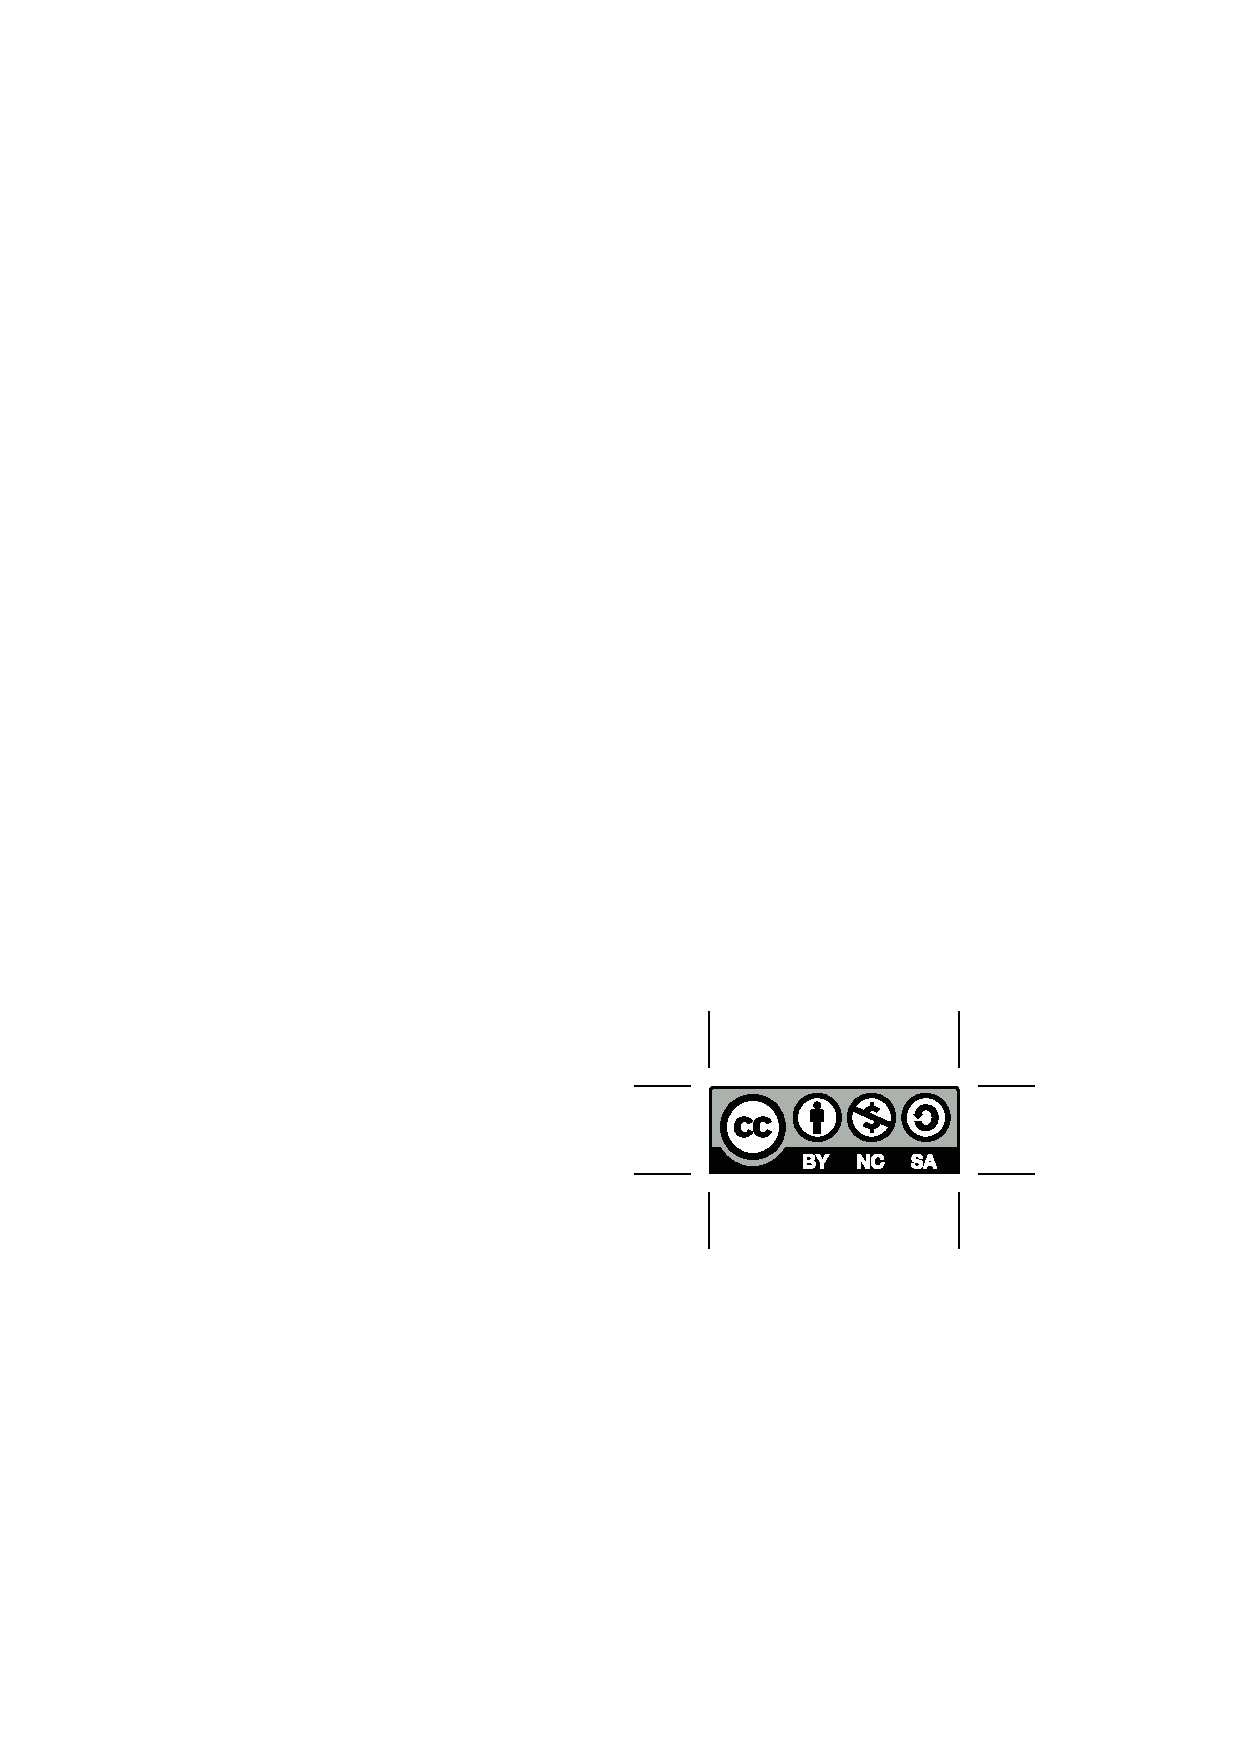
\includegraphics[scale = 0.8]{img/by-nc-sa}}
\end{center}
\fi

Il progetto è ospitato su GitHub, dove si può trovare la versione più recente, al link \url{https://github.com/SciSNS-2017/Sistemi-Dinamici}. Ogni suggerimento (errori, soluzioni di esercizi, contributi vari, ecc.) è sempre gradito e può essere segnalato creando una \emph{issue} su GitHub oppure contattando direttamente gli autori.

\tableofcontents

\mainmatter
\chapter{Lezioni}
\section{Lezione del 09/10/2018}
\begin{definition}[gruppo]
	Un gruppo è una coppia $ \mathcal{G} \coloneqq (G, \star) $ dove $ G $ è un insieme e $ + \colon G \times G \to G $ è un'operazione binaria che gode delle seguenti proprietà
	\begin{enumerate}[label=(\roman*)]
		\item \emph{associativa}: $ \forall g_1, g_2, g_3 \in G, \ g_1 \star (g_2 \star g_3) = (g_1 \star g_2) \star g_3 $;
		\item \emph{elemento neutro sinistro}: $  \exists e \in G : \forall g \in G, \ g \star e = g $;
		\item \emph{inverso sinistro}: $ \forall g \in G, \exists g^{-1} \in G : g \star g^{-1} = e $.
	\end{enumerate}
	A partire da queste si mostra facilmente che l'elemento neutro destro è anche elemento neutro sinistro, l'inverso destro è anche inverso sinistro, che l'elemento neutro e l'inverso sono unici. \\
	Se non ci sono ambiguità circa l'operazione definita su $ G $ indicheremo più semplicemente il gruppo $ \mathcal{G} $ facendo riferimento al solo insieme $ G $. 
\end{definition}

\begin{definition}[sistema dinamico]
	Un sistema dinamico è una terna $ (\mathcal{G}, \mathcal{X}, \Phi) $ dove $ \mathcal{G} \coloneqq (G, \star) $ è un (semi-)gruppo, $ \mathcal{X} $ è uno spazio, cioè un insieme $ X $ dotato di una qualche struttura (per esempio una topologia), e 
	\begin{align*}
		\Phi \colon G \times X & \to X \\
		(g, x) & \mapsto \Phi(g, x) = \Phi_g(x)
	\end{align*}
	è una applicazione tale che
	\begin{enumerate}[label=(\roman*)]
		\item $ \forall x \in X, \ \Phi_e(x) = x $ dove $ e $ è l'elemento neutro di $ G $, cioè $ \Phi_e = \Id_X $;
		\item $ \forall g_1, g_2 \in G, \forall x \in X, \ \Phi_{(g_1 \star g_2)}(x) = (\Phi_{g1} \circ \Phi_{g_2})(x) $ cioè $ \Phi_{(g_1 \star g_2)} = \Phi_{g1} \circ \Phi_{g_2} $.
	\end{enumerate}
	Più brevemente diciamo che un sistema dinamico è l'\emph{azione} di un gruppo $ G $ su uno spazio $ X $ definita da una mappa $ \Phi $. 
\end{definition}

Nella maggior parte dei casi useremo come gruppo insiemi numerici $ \N $, $ \Z $ e $ \R $ con le usuali operazioni. Nei primi due casi parleremo di sistemi a \emph{tempo discreto} mentre nell'ultimo di sistemi a \emph{tempo continuo}. Come spazio $ \mathcal{X} $ useremo spesso uno \emph{spazio metrico compatto} (e.g. la sfera $ \S^d $, il toro $ \T^d $ o un intervallo chiuso $ [a, b] $), uno \emph{spazio di probabilità} o gli insiemi $ \R^d $ e $ \C $ con le usuali strutture. \\

Per quanto riguarda la mappa $ \Phi $ osserviamo che per definizione $ \Phi_g \in \End{(X)} $ ovvero è un \emph{endomorfismo} su $ X $. Tuttavia spesso penseremo a $ \Phi_g \in \Aut{(X)} $ ovvero un \emph{automorfismo} cioè un endomorfismo invertibile. \\

Sia $ f \in \End{(X)} $. Dato $ n \in \N $ poniamo $ f^n \coloneqq f \circ \cdots \circ f $ ($ f $ composta $ n $ volte) con la convenzione che $ f^1 = f $ e $ f^0 = \Id_X $. Se consideriamo $ \N $ con l'operazione di addizione, l'applicazione $ \Phi^f $ data da $ \Phi_n^f(x) \coloneqq f^n(x) $ definisce un sistema dinamico. \\
Se prendiamo $ f \in \Aut{(X)} $ possiamo considerare la stessa costruzione usando come gruppo $ \Z $ e definendo $ f^{-n} $ come l'inversa di $ f^n $. 

\begin{example}
	Partendo dalla costruzione appena data possiamo prendere $ X = [0, 1] $ e per $ \alpha \in \R $ la funzione $ f(x) \coloneqq x + \alpha \pmod{1} $. Osserviamo che essendo $ f $ invertibile possiamo definire l'applicazione $ \Phi $ su $ \Z $. Il sistema così definito è un prototipo di \emph{sistema periodico} se $ \alpha \in \Q $ e di \emph{sistema quasi-periodico} se $ \alpha \notin \Q $. \\
	\texttt{Sarebbe carino mettere un'immagine.}
\end{example}

Prendiamo come gruppo $ \R $ o $ [0, +\infty) $. In tale caso data l'applicazione $ \Phi_t(x) = \Phi(t, x) $ prende il nome di \emph{flusso} o \emph{semi-flusso} rispettivamente. \\

Un esempio di sistema dinamico a tempo continuo è dato da un'equazione differenziale ordinaria (ODE) del primo ordine \footnote{Di seguito considereremo quasi solo ODE del primo ordine in quanto equazioni differenziali di ordine superiore possono essere ricondotte a questa con il solito cambio di variabile a sistemi di ODE del primo ordine.} autonoma
\begin{equation}
	\begin{cases}
		\dot{x} = v(x) \\
		x(0) = x_0
	\end{cases}
\end{equation} 
dove $ x, x_0 \in \R^n $ e $ v \colon \R^n \to \R^n $ è un campo vettoriale. Se supponiamo che $ v $ sia di classe $ \mathcal{C}^1 $ allora abbiamo esistenza e unicità della soluzione \texttt{(e dipendenza continua dai parametri iniziali ??)}, cioè esiste $ \tau > 0 $ e un'unica funzione $ \phi \colon [0, \tau) \to \R^n $ tale che $ \phi(0) = x_0 $ e $ \phi'(t) = v(\phi(0)) $ per ogni $ t \in [0, \tau) $. \\
Se supponiamo per esempio che $ v $ sia un'applicazione lineare $ v(x) \coloneqq A x $ con $ A \in \mathrm{Mat}_{n \times n}(\R) $ allora abbiamo che la soluzione è prolungabile a tutto l'asse reale e introducendo la nozione di esponenziale di una matrice %
\footnote{%
	Data $ A \in \mathrm{Mat}_{n \times n}(\R) $ si pone 
	\[
		\exp(A) \coloneqq \sum_{k = 0}^{+\infty} \frac{A^k}{k!}.
	\] 
} si può scrivere nella forma 
\[
	\phi(t) = \exp{\left(t \, A\right)} \, x_0. 
\]


\begin{definition}[orbita e spazio delle orbite]
	Data $ f \in \Aut{(X)} $ e $ \Phi^f \colon \Z \times X \to X $ definiamo orbita di $ x \in X $ come 
	\[
	\mathcal{O}^f(x) \coloneqq \{f^n(x) : n \in \Z\}.
	\]
	Le orbite definiscono una naturale relazione di equivalenza $ x \sim y \iff \exists n \in \Z : y = f^n(x) \iff y \in \mathcal{O}^f(x) \iff x \in \mathcal{O}^f(y) $. Chiamiamo lo spazio quoziente $ \faktor{X}{\sim} $ spazio delle orbite. \texttt{Topologia quoziente?}
\end{definition}

Pendolo semplice...

\section{Lezione del 10/10/2018}
\subsection{Introduzione}
La Teoria della Misura nasce a inizio '900 per formalizzare la probabilità e per cercare di fondare una teoria dell'integrazione che risulti più efficace di quella di Riemann. Per alcuni sottoinsiemi di $\R$, in particolare per gli intervalli limitati, abbiamo un concetto intuitivo di "misura", ovvero la lunghezza dell'intervallo:
\[\lambda\left([a,b]\right) = b-a.\]
L'obiettivo della teoria della misura è estendere questa nozione ad altri sottoinsiemi di $\R$ in modo coerente, ovvero in modo da rispettare, ad esempio, la proprietà di additività:
\[A \cap B = \emptyset \implies \lambda(A\cup B) = \lambda(A) + \lambda(B)\]
\section{Lezione del 16/10/2018 [Marmi]}
\begin{definition}[orbita pre-periodica e periodica] Sia $f\colon X \to X$ un sistema dinamico. Un'orbita $\mathcal{O}^f(x)$ si dice pre-periodica se contiene un numero finito di elementi. Se inoltre $ f $ è invertibile l'orbita si dice periodica e la sua cardinalità si dice periodo. \\
Infine, se $f$ non è invertibile, possono esistere punti $ x $ (che costituiscono il pre-periodo) tali che $ \forall n > 0\ f^n (x) \neq x $.
\end{definition}

\begin{example}[Congettura di Collatz]
Si consideri il sistema dinamico $f \colon \N \to \N$:
\[
    f(n) \coloneqq
    \begin{cases}
        n/2  & \text{se $ n $ è pari}    \\
        3n+1 & \text{se $ n $ è dispari}
    \end{cases}
\]
La congettura\footnote{È attualmente un problema aperto.} di Collatz asserisce che tutti gli $n \in \N$ sono preperiodici e che l'unico ciclo è $ 1 \to 4 \to 2 \to 1 $.
\end{example}

\subsection{Coniugazione e misure invarianti}
\begin{definition}[Sistemi dinamici coniugati]
Siano $f\colon X \to X$ e $g\colon Y \to Y$ due sistemi dinamici. Questi si dicono coniugati se esiste $h \colon X \to Y$ invertibile tale che $h \circ f = g \circ h$, cioè tale da far commutare il seguente diagramma:
\begin{center}
    \begin{tikzcd}
        X \arrow[r, "f"] \arrow[d, "h"]  & X \arrow[d, "h"] \\
        Y \arrow[r, "g"] & Y
    \end{tikzcd}
\end{center}
Se $h$ è solamente surgettiva si dice che $g$ è un \emph{fattore} di $f$ oppure che $f$ è un'\emph{estensione} di $g$. Se invece $h$ è solo iniettiva allora si dice che $f$ è un \emph{sottosistema} di $g$.
\end{definition}

\begin{example} \label{ex:Ulam_Mandelbrot}
Si considerino i seguenti sistemi dinamici $ \C \to \C$:
\[ Q_\lambda(z) \coloneqq \lambda z (1-z) \]
\[ P_c(z) \coloneqq z^2 + c \qquad \text{con } c = - \frac{\lambda^2}{4} +  \frac{\lambda}{2}. \]
Le funzioni $ Q_\lambda $ sono dette \emph{trasformazioni di Ulam-Von Neumann}, mentre $P_c$ è la funzione che genera l'\emph{insieme di Mandelbrot}.
I due sistemi risultano coniugati attraverso la funzione
\[ h_\lambda(z) = -\lambda z + \frac{\lambda}{2}\;. \]
Infatti si verifica che $ h\circ Q_\lambda = P_c \circ h $.
\end{example}

\begin{example} \label{ex:Ulam_tenda}
    Sia $ Q_4 \colon [0,1] \to [0,1] $ come definita nell'esempio \ref{ex:Ulam_Mandelbrot} e sia $ T\colon [0,1] \to [0,1] $ la mappa a tenda:
    \[
        T(x) \coloneqq
        \begin{cases}
            2x   & \text{se } 0 \leq x \leq 1/2 \\
            2-2x & \text{se } 1/2 \leq x \leq 1
        \end{cases}.
    \]
    Allora i due sistemi sono coniugati tramite $ h(x) = \sin^2\left(\frac{\pi x}{2}\right) $, cioè si ha $ Q_4\circ h = h\circ T $.
    Inoltre, poiché $ T $ conserva la misura di Lebesgue, usando la \eqref{eq:pushforward-misure} si ottiene che $ Q_4 $ conserva la misura:
    \[ \dif{h_\sharp \lambda}(x) = \frac{\dif x}{\pi\sqrt{x(1-x)}}\; . \]

    \iffigureon
    \begin{figure}
        \begin{center}
            \subfloat[Mappa a tenda]
            { \definecolor{qqqqcc}{rgb}{0.,0.,0.8}
\begin{tikzpicture}[line cap=round,line join=round,>=triangle 45,x=5.0cm,y=5.0cm]
\draw[->,color=black] (-0.1,0.) -- (1.1,0.);
\foreach \x in {,0.2,0.4,0.6,0.8,1.}
\draw[shift={(\x,0)},color=black] (0pt,2pt) -- (0pt,-2pt) node[below] {\footnotesize $\x$};
\draw[->,color=black] (0.,-0.1) -- (0.,1.1);
\foreach \y in {,0.2,0.4,0.6,0.8,1.}
\draw[shift={(0,\y)},color=black] (2pt,0pt) -- (-2pt,0pt) node[left] {\footnotesize $\y$};
\draw[color=black] (0pt,-10pt) node[right] {\footnotesize $0$};
\clip(-0.1,-0.1) rectangle (1.1,1.1);
\draw[line width=1pt,color=qqqqcc] (8.000000000003847E-7,0.0) -- (0.0,0.0);
\draw[line width=1pt,color=qqqqcc] (0.0,0.0) -- (0.0024999956818200016,0.004999991363640003);
\draw[line width=1pt,color=qqqqcc] (0.0024999956818200016,0.004999991363640003) -- (0.004999991363640003,0.009999982727280006);
\draw[line width=1pt,color=qqqqcc] (0.004999991363640003,0.009999982727280006) -- (0.007499987045460005,0.01499997409092001);
\draw[line width=1pt,color=qqqqcc] (0.007499987045460005,0.01499997409092001) -- (0.009999982727280006,0.019999965454560013);
\draw[line width=1pt,color=qqqqcc] (0.009999982727280006,0.019999965454560013) -- (0.012499978409100007,0.024999956818200015);
\draw[line width=1pt,color=qqqqcc] (0.012499978409100007,0.024999956818200015) -- (0.014999974090920009,0.029999948181840017);
\draw[line width=1pt,color=qqqqcc] (0.014999974090920009,0.029999948181840017) -- (0.01749996977274001,0.03499993954548002);
\draw[line width=1pt,color=qqqqcc] (0.01749996977274001,0.03499993954548002) -- (0.019999965454560013,0.039999930909120025);
\draw[line width=1pt,color=qqqqcc] (0.019999965454560013,0.039999930909120025) -- (0.022499961136380014,0.04499992227276003);
\draw[line width=1pt,color=qqqqcc] (0.022499961136380014,0.04499992227276003) -- (0.024999956818200015,0.04999991363640003);
\draw[line width=1pt,color=qqqqcc] (0.024999956818200015,0.04999991363640003) -- (0.027499952500020016,0.05499990500004003);
\draw[line width=1pt,color=qqqqcc] (0.027499952500020016,0.05499990500004003) -- (0.029999948181840017,0.059999896363680034);
\draw[line width=1pt,color=qqqqcc] (0.029999948181840017,0.059999896363680034) -- (0.03249994386366002,0.06499988772732004);
\draw[line width=1pt,color=qqqqcc] (0.03249994386366002,0.06499988772732004) -- (0.03499993954548002,0.06999987909096005);
\draw[line width=1pt,color=qqqqcc] (0.03499993954548002,0.06999987909096005) -- (0.037499935227300024,0.07499987045460005);
\draw[line width=1pt,color=qqqqcc] (0.037499935227300024,0.07499987045460005) -- (0.039999930909120025,0.07999986181824005);
\draw[line width=1pt,color=qqqqcc] (0.039999930909120025,0.07999986181824005) -- (0.042499926590940026,0.08499985318188005);
\draw[line width=1pt,color=qqqqcc] (0.042499926590940026,0.08499985318188005) -- (0.04499992227276003,0.08999984454552006);
\draw[line width=1pt,color=qqqqcc] (0.04499992227276003,0.08999984454552006) -- (0.04749991795458003,0.09499983590916006);
\draw[line width=1pt,color=qqqqcc] (0.04749991795458003,0.09499983590916006) -- (0.04999991363640003,0.09999982727280006);
\draw[line width=1pt,color=qqqqcc] (0.04999991363640003,0.09999982727280006) -- (0.05249990931822003,0.10499981863644006);
\draw[line width=1pt,color=qqqqcc] (0.05249990931822003,0.10499981863644006) -- (0.05499990500004003,0.10999981000008006);
\draw[line width=1pt,color=qqqqcc] (0.05499990500004003,0.10999981000008006) -- (0.05749990068186003,0.11499980136372007);
\draw[line width=1pt,color=qqqqcc] (0.05749990068186003,0.11499980136372007) -- (0.059999896363680034,0.11999979272736007);
\draw[line width=1pt,color=qqqqcc] (0.059999896363680034,0.11999979272736007) -- (0.062499892045500036,0.12499978409100007);
\draw[line width=1pt,color=qqqqcc] (0.062499892045500036,0.12499978409100007) -- (0.06499988772732004,0.1299997754546401);
\draw[line width=1pt,color=qqqqcc] (0.06499988772732004,0.1299997754546401) -- (0.06749988340914005,0.1349997668182801);
\draw[line width=1pt,color=qqqqcc] (0.06749988340914005,0.1349997668182801) -- (0.06999987909096006,0.13999975818192012);
\draw[line width=1pt,color=qqqqcc] (0.06999987909096006,0.13999975818192012) -- (0.07249987477278007,0.14499974954556014);
\draw[line width=1pt,color=qqqqcc] (0.07249987477278007,0.14499974954556014) -- (0.07499987045460008,0.14999974090920015);
\draw[line width=1pt,color=qqqqcc] (0.07499987045460008,0.14999974090920015) -- (0.07749986613642008,0.15499973227284017);
\draw[line width=1pt,color=qqqqcc] (0.07749986613642008,0.15499973227284017) -- (0.07999986181824009,0.15999972363648018);
\draw[line width=1pt,color=qqqqcc] (0.07999986181824009,0.15999972363648018) -- (0.0824998575000601,0.1649997150001202);
\draw[line width=1pt,color=qqqqcc] (0.0824998575000601,0.1649997150001202) -- (0.08499985318188011,0.16999970636376022);
\draw[line width=1pt,color=qqqqcc] (0.08499985318188011,0.16999970636376022) -- (0.08749984886370012,0.17499969772740023);
\draw[line width=1pt,color=qqqqcc] (0.08749984886370012,0.17499969772740023) -- (0.08999984454552012,0.17999968909104025);
\draw[line width=1pt,color=qqqqcc] (0.08999984454552012,0.17999968909104025) -- (0.09249984022734013,0.18499968045468027);
\draw[line width=1pt,color=qqqqcc] (0.09249984022734013,0.18499968045468027) -- (0.09499983590916014,0.18999967181832028);
\draw[line width=1pt,color=qqqqcc] (0.09499983590916014,0.18999967181832028) -- (0.09749983159098015,0.1949996631819603);
\draw[line width=1pt,color=qqqqcc] (0.09749983159098015,0.1949996631819603) -- (0.09999982727280016,0.1999996545456003);
\draw[line width=1pt,color=qqqqcc] (0.09999982727280016,0.1999996545456003) -- (0.10249982295462017,0.20499964590924033);
\draw[line width=1pt,color=qqqqcc] (0.10249982295462017,0.20499964590924033) -- (0.10499981863644017,0.20999963727288035);
\draw[line width=1pt,color=qqqqcc] (0.10499981863644017,0.20999963727288035) -- (0.10749981431826018,0.21499962863652036);
\draw[line width=1pt,color=qqqqcc] (0.10749981431826018,0.21499962863652036) -- (0.10999981000008019,0.21999962000016038);
\draw[line width=1pt,color=qqqqcc] (0.10999981000008019,0.21999962000016038) -- (0.1124998056819002,0.2249996113638004);
\draw[line width=1pt,color=qqqqcc] (0.1124998056819002,0.2249996113638004) -- (0.1149998013637202,0.2299996027274404);
\draw[line width=1pt,color=qqqqcc] (0.1149998013637202,0.2299996027274404) -- (0.11749979704554021,0.23499959409108043);
\draw[line width=1pt,color=qqqqcc] (0.11749979704554021,0.23499959409108043) -- (0.11999979272736022,0.23999958545472044);
\draw[line width=1pt,color=qqqqcc] (0.11999979272736022,0.23999958545472044) -- (0.12249978840918023,0.24499957681836046);
\draw[line width=1pt,color=qqqqcc] (0.12249978840918023,0.24499957681836046) -- (0.12499978409100024,0.24999956818200048);
\draw[line width=1pt,color=qqqqcc] (0.12499978409100024,0.24999956818200048) -- (0.12749977977282023,0.25499955954564046);
\draw[line width=1pt,color=qqqqcc] (0.12749977977282023,0.25499955954564046) -- (0.12999977545464023,0.25999955090928045);
\draw[line width=1pt,color=qqqqcc] (0.12999977545464023,0.25999955090928045) -- (0.13249977113646022,0.26499954227292044);
\draw[line width=1pt,color=qqqqcc] (0.13249977113646022,0.26499954227292044) -- (0.13499976681828021,0.26999953363656043);
\draw[line width=1pt,color=qqqqcc] (0.13499976681828021,0.26999953363656043) -- (0.1374997625001002,0.2749995250002004);
\draw[line width=1pt,color=qqqqcc] (0.1374997625001002,0.2749995250002004) -- (0.1399997581819202,0.2799995163638404);
\draw[line width=1pt,color=qqqqcc] (0.1399997581819202,0.2799995163638404) -- (0.1424997538637402,0.2849995077274804);
\draw[line width=1pt,color=qqqqcc] (0.1424997538637402,0.2849995077274804) -- (0.1449997495455602,0.2899994990911204);
\draw[line width=1pt,color=qqqqcc] (0.1449997495455602,0.2899994990911204) -- (0.14749974522738019,0.29499949045476037);
\draw[line width=1pt,color=qqqqcc] (0.14749974522738019,0.29499949045476037) -- (0.14999974090920018,0.29999948181840036);
\draw[line width=1pt,color=qqqqcc] (0.14999974090920018,0.29999948181840036) -- (0.15249973659102017,0.30499947318204035);
\draw[line width=1pt,color=qqqqcc] (0.15249973659102017,0.30499947318204035) -- (0.15499973227284017,0.30999946454568034);
\draw[line width=1pt,color=qqqqcc] (0.15499973227284017,0.30999946454568034) -- (0.15749972795466016,0.3149994559093203);
\draw[line width=1pt,color=qqqqcc] (0.15749972795466016,0.3149994559093203) -- (0.15999972363648016,0.3199994472729603);
\draw[line width=1pt,color=qqqqcc] (0.15999972363648016,0.3199994472729603) -- (0.16249971931830015,0.3249994386366003);
\draw[line width=1pt,color=qqqqcc] (0.16249971931830015,0.3249994386366003) -- (0.16499971500012015,0.3299994300002403);
\draw[line width=1pt,color=qqqqcc] (0.16499971500012015,0.3299994300002403) -- (0.16749971068194014,0.3349994213638803);
\draw[line width=1pt,color=qqqqcc] (0.16749971068194014,0.3349994213638803) -- (0.16999970636376013,0.33999941272752027);
\draw[line width=1pt,color=qqqqcc] (0.16999970636376013,0.33999941272752027) -- (0.17249970204558013,0.34499940409116026);
\draw[line width=1pt,color=qqqqcc] (0.17249970204558013,0.34499940409116026) -- (0.17499969772740012,0.34999939545480024);
\draw[line width=1pt,color=qqqqcc] (0.17499969772740012,0.34999939545480024) -- (0.17749969340922012,0.35499938681844023);
\draw[line width=1pt,color=qqqqcc] (0.17749969340922012,0.35499938681844023) -- (0.1799996890910401,0.3599993781820802);
\draw[line width=1pt,color=qqqqcc] (0.1799996890910401,0.3599993781820802) -- (0.1824996847728601,0.3649993695457202);
\draw[line width=1pt,color=qqqqcc] (0.1824996847728601,0.3649993695457202) -- (0.1849996804546801,0.3699993609093602);
\draw[line width=1pt,color=qqqqcc] (0.1849996804546801,0.3699993609093602) -- (0.1874996761365001,0.3749993522730002);
\draw[line width=1pt,color=qqqqcc] (0.1874996761365001,0.3749993522730002) -- (0.1899996718183201,0.3799993436366402);
\draw[line width=1pt,color=qqqqcc] (0.1899996718183201,0.3799993436366402) -- (0.19249966750014008,0.38499933500028016);
\draw[line width=1pt,color=qqqqcc] (0.19249966750014008,0.38499933500028016) -- (0.19499966318196008,0.38999932636392015);
\draw[line width=1pt,color=qqqqcc] (0.19499966318196008,0.38999932636392015) -- (0.19749965886378007,0.39499931772756014);
\draw[line width=1pt,color=qqqqcc] (0.19749965886378007,0.39499931772756014) -- (0.19999965454560006,0.39999930909120013);
\draw[line width=1pt,color=qqqqcc] (0.19999965454560006,0.39999930909120013) -- (0.20249965022742006,0.4049993004548401);
\draw[line width=1pt,color=qqqqcc] (0.20249965022742006,0.4049993004548401) -- (0.20499964590924005,0.4099992918184801);
\draw[line width=1pt,color=qqqqcc] (0.20499964590924005,0.4099992918184801) -- (0.20749964159106005,0.4149992831821201);
\draw[line width=1pt,color=qqqqcc] (0.20749964159106005,0.4149992831821201) -- (0.20999963727288004,0.4199992745457601);
\draw[line width=1pt,color=qqqqcc] (0.20999963727288004,0.4199992745457601) -- (0.21249963295470004,0.42499926590940007);
\draw[line width=1pt,color=qqqqcc] (0.21249963295470004,0.42499926590940007) -- (0.21499962863652003,0.42999925727304006);
\draw[line width=1pt,color=qqqqcc] (0.21499962863652003,0.42999925727304006) -- (0.21749962431834002,0.43499924863668005);
\draw[line width=1pt,color=qqqqcc] (0.21749962431834002,0.43499924863668005) -- (0.21999962000016002,0.43999924000032004);
\draw[line width=1pt,color=qqqqcc] (0.21999962000016002,0.43999924000032004) -- (0.22249961568198,0.44499923136396);
\draw[line width=1pt,color=qqqqcc] (0.22249961568198,0.44499923136396) -- (0.2249996113638,0.4499992227276);
\draw[line width=1pt,color=qqqqcc] (0.2249996113638,0.4499992227276) -- (0.22749960704562,0.45499921409124);
\draw[line width=1pt,color=qqqqcc] (0.22749960704562,0.45499921409124) -- (0.22999960272744,0.45999920545488);
\draw[line width=1pt,color=qqqqcc] (0.22999960272744,0.45999920545488) -- (0.23249959840926,0.46499919681852);
\draw[line width=1pt,color=qqqqcc] (0.23249959840926,0.46499919681852) -- (0.23499959409107998,0.46999918818215997);
\draw[line width=1pt,color=qqqqcc] (0.23499959409107998,0.46999918818215997) -- (0.23749958977289998,0.47499917954579995);
\draw[line width=1pt,color=qqqqcc] (0.23749958977289998,0.47499917954579995) -- (0.23999958545471997,0.47999917090943994);
\draw[line width=1pt,color=qqqqcc] (0.23999958545471997,0.47999917090943994) -- (0.24249958113653997,0.48499916227307993);
\draw[line width=1pt,color=qqqqcc] (0.24249958113653997,0.48499916227307993) -- (0.24499957681835996,0.4899991536367199);
\draw[line width=1pt,color=qqqqcc] (0.24499957681835996,0.4899991536367199) -- (0.24749957250017995,0.4949991450003599);
\draw[line width=1pt,color=qqqqcc] (0.24749957250017995,0.4949991450003599) -- (0.24999956818199995,0.4999991363639999);
\draw[line width=1pt,color=qqqqcc] (0.24999956818199995,0.4999991363639999) -- (0.25249956386381994,0.5049991277276399);
\draw[line width=1pt,color=qqqqcc] (0.25249956386381994,0.5049991277276399) -- (0.25499955954563996,0.5099991190912799);
\draw[line width=1pt,color=qqqqcc] (0.25499955954563996,0.5099991190912799) -- (0.25749955522746,0.51499911045492);
\draw[line width=1pt,color=qqqqcc] (0.25749955522746,0.51499911045492) -- (0.25999955090928,0.51999910181856);
\draw[line width=1pt,color=qqqqcc] (0.25999955090928,0.51999910181856) -- (0.26249954659110003,0.5249990931822001);
\draw[line width=1pt,color=qqqqcc] (0.26249954659110003,0.5249990931822001) -- (0.26499954227292005,0.5299990845458401);
\draw[line width=1pt,color=qqqqcc] (0.26499954227292005,0.5299990845458401) -- (0.2674995379547401,0.5349990759094801);
\draw[line width=1pt,color=qqqqcc] (0.2674995379547401,0.5349990759094801) -- (0.2699995336365601,0.5399990672731202);
\draw[line width=1pt,color=qqqqcc] (0.2699995336365601,0.5399990672731202) -- (0.2724995293183801,0.5449990586367602);
\draw[line width=1pt,color=qqqqcc] (0.2724995293183801,0.5449990586367602) -- (0.27499952500020014,0.5499990500004003);
\draw[line width=1pt,color=qqqqcc] (0.27499952500020014,0.5499990500004003) -- (0.27749952068202016,0.5549990413640403);
\draw[line width=1pt,color=qqqqcc] (0.27749952068202016,0.5549990413640403) -- (0.2799995163638402,0.5599990327276804);
\draw[line width=1pt,color=qqqqcc] (0.2799995163638402,0.5599990327276804) -- (0.2824995120456602,0.5649990240913204);
\draw[line width=1pt,color=qqqqcc] (0.2824995120456602,0.5649990240913204) -- (0.28499950772748023,0.5699990154549605);
\draw[line width=1pt,color=qqqqcc] (0.28499950772748023,0.5699990154549605) -- (0.28749950340930025,0.5749990068186005);
\draw[line width=1pt,color=qqqqcc] (0.28749950340930025,0.5749990068186005) -- (0.28999949909112027,0.5799989981822405);
\draw[line width=1pt,color=qqqqcc] (0.28999949909112027,0.5799989981822405) -- (0.2924994947729403,0.5849989895458806);
\draw[line width=1pt,color=qqqqcc] (0.2924994947729403,0.5849989895458806) -- (0.2949994904547603,0.5899989809095206);
\draw[line width=1pt,color=qqqqcc] (0.2949994904547603,0.5899989809095206) -- (0.29749948613658034,0.5949989722731607);
\draw[line width=1pt,color=qqqqcc] (0.29749948613658034,0.5949989722731607) -- (0.29999948181840036,0.5999989636368007);
\draw[line width=1pt,color=qqqqcc] (0.29999948181840036,0.5999989636368007) -- (0.3024994775002204,0.6049989550004408);
\draw[line width=1pt,color=qqqqcc] (0.3024994775002204,0.6049989550004408) -- (0.3049994731820404,0.6099989463640808);
\draw[line width=1pt,color=qqqqcc] (0.3049994731820404,0.6099989463640808) -- (0.3074994688638604,0.6149989377277209);
\draw[line width=1pt,color=qqqqcc] (0.3074994688638604,0.6149989377277209) -- (0.30999946454568045,0.6199989290913609);
\draw[line width=1pt,color=qqqqcc] (0.30999946454568045,0.6199989290913609) -- (0.31249946022750047,0.6249989204550009);
\draw[line width=1pt,color=qqqqcc] (0.31249946022750047,0.6249989204550009) -- (0.3149994559093205,0.629998911818641);
\draw[line width=1pt,color=qqqqcc] (0.3149994559093205,0.629998911818641) -- (0.3174994515911405,0.634998903182281);
\draw[line width=1pt,color=qqqqcc] (0.3174994515911405,0.634998903182281) -- (0.31999944727296054,0.6399988945459211);
\draw[line width=1pt,color=qqqqcc] (0.31999944727296054,0.6399988945459211) -- (0.32249944295478056,0.6449988859095611);
\draw[line width=1pt,color=qqqqcc] (0.32249944295478056,0.6449988859095611) -- (0.3249994386366006,0.6499988772732012);
\draw[line width=1pt,color=qqqqcc] (0.3249994386366006,0.6499988772732012) -- (0.3274994343184206,0.6549988686368412);
\draw[line width=1pt,color=qqqqcc] (0.3274994343184206,0.6549988686368412) -- (0.3299994300002406,0.6599988600004812);
\draw[line width=1pt,color=qqqqcc] (0.3299994300002406,0.6599988600004812) -- (0.33249942568206065,0.6649988513641213);
\draw[line width=1pt,color=qqqqcc] (0.33249942568206065,0.6649988513641213) -- (0.33499942136388067,0.6699988427277613);
\draw[line width=1pt,color=qqqqcc] (0.33499942136388067,0.6699988427277613) -- (0.3374994170457007,0.6749988340914014);
\draw[line width=1pt,color=qqqqcc] (0.3374994170457007,0.6749988340914014) -- (0.3399994127275207,0.6799988254550414);
\draw[line width=1pt,color=qqqqcc] (0.3399994127275207,0.6799988254550414) -- (0.34249940840934073,0.6849988168186815);
\draw[line width=1pt,color=qqqqcc] (0.34249940840934073,0.6849988168186815) -- (0.34499940409116076,0.6899988081823215);
\draw[line width=1pt,color=qqqqcc] (0.34499940409116076,0.6899988081823215) -- (0.3474993997729808,0.6949987995459616);
\draw[line width=1pt,color=qqqqcc] (0.3474993997729808,0.6949987995459616) -- (0.3499993954548008,0.6999987909096016);
\draw[line width=1pt,color=qqqqcc] (0.3499993954548008,0.6999987909096016) -- (0.3524993911366208,0.7049987822732416);
\draw[line width=1pt,color=qqqqcc] (0.3524993911366208,0.7049987822732416) -- (0.35499938681844084,0.7099987736368817);
\draw[line width=1pt,color=qqqqcc] (0.35499938681844084,0.7099987736368817) -- (0.35749938250026086,0.7149987650005217);
\draw[line width=1pt,color=qqqqcc] (0.35749938250026086,0.7149987650005217) -- (0.3599993781820809,0.7199987563641618);
\draw[line width=1pt,color=qqqqcc] (0.3599993781820809,0.7199987563641618) -- (0.3624993738639009,0.7249987477278018);
\draw[line width=1pt,color=qqqqcc] (0.3624993738639009,0.7249987477278018) -- (0.36499936954572093,0.7299987390914419);
\draw[line width=1pt,color=qqqqcc] (0.36499936954572093,0.7299987390914419) -- (0.36749936522754095,0.7349987304550819);
\draw[line width=1pt,color=qqqqcc] (0.36749936522754095,0.7349987304550819) -- (0.369999360909361,0.739998721818722);
\draw[line width=1pt,color=qqqqcc] (0.369999360909361,0.739998721818722) -- (0.372499356591181,0.744998713182362);
\draw[line width=1pt,color=qqqqcc] (0.372499356591181,0.744998713182362) -- (0.374999352273001,0.749998704546002);
\draw[line width=1pt,color=qqqqcc] (0.374999352273001,0.749998704546002) -- (0.37749934795482104,0.7549986959096421);
\draw[line width=1pt,color=qqqqcc] (0.37749934795482104,0.7549986959096421) -- (0.37999934363664106,0.7599986872732821);
\draw[line width=1pt,color=qqqqcc] (0.37999934363664106,0.7599986872732821) -- (0.3824993393184611,0.7649986786369222);
\draw[line width=1pt,color=qqqqcc] (0.3824993393184611,0.7649986786369222) -- (0.3849993350002811,0.7699986700005622);
\draw[line width=1pt,color=qqqqcc] (0.3849993350002811,0.7699986700005622) -- (0.38749933068210113,0.7749986613642023);
\draw[line width=1pt,color=qqqqcc] (0.38749933068210113,0.7749986613642023) -- (0.38999932636392115,0.7799986527278423);
\draw[line width=1pt,color=qqqqcc] (0.38999932636392115,0.7799986527278423) -- (0.3924993220457412,0.7849986440914823);
\draw[line width=1pt,color=qqqqcc] (0.3924993220457412,0.7849986440914823) -- (0.3949993177275612,0.7899986354551224);
\draw[line width=1pt,color=qqqqcc] (0.3949993177275612,0.7899986354551224) -- (0.3974993134093812,0.7949986268187624);
\draw[line width=1pt,color=qqqqcc] (0.3974993134093812,0.7949986268187624) -- (0.39999930909120124,0.7999986181824025);
\draw[line width=1pt,color=qqqqcc] (0.39999930909120124,0.7999986181824025) -- (0.40249930477302126,0.8049986095460425);
\draw[line width=1pt,color=qqqqcc] (0.40249930477302126,0.8049986095460425) -- (0.4049993004548413,0.8099986009096826);
\draw[line width=1pt,color=qqqqcc] (0.4049993004548413,0.8099986009096826) -- (0.4074992961366613,0.8149985922733226);
\draw[line width=1pt,color=qqqqcc] (0.4074992961366613,0.8149985922733226) -- (0.4099992918184813,0.8199985836369627);
\draw[line width=1pt,color=qqqqcc] (0.4099992918184813,0.8199985836369627) -- (0.41249928750030135,0.8249985750006027);
\draw[line width=1pt,color=qqqqcc] (0.41249928750030135,0.8249985750006027) -- (0.41499928318212137,0.8299985663642427);
\draw[line width=1pt,color=qqqqcc] (0.41499928318212137,0.8299985663642427) -- (0.4174992788639414,0.8349985577278828);
\draw[line width=1pt,color=qqqqcc] (0.4174992788639414,0.8349985577278828) -- (0.4199992745457614,0.8399985490915228);
\draw[line width=1pt,color=qqqqcc] (0.4199992745457614,0.8399985490915228) -- (0.42249927022758144,0.8449985404551629);
\draw[line width=1pt,color=qqqqcc] (0.42249927022758144,0.8449985404551629) -- (0.42499926590940146,0.8499985318188029);
\draw[line width=1pt,color=qqqqcc] (0.42499926590940146,0.8499985318188029) -- (0.4274992615912215,0.854998523182443);
\draw[line width=1pt,color=qqqqcc] (0.4274992615912215,0.854998523182443) -- (0.4299992572730415,0.859998514546083);
\draw[line width=1pt,color=qqqqcc] (0.4299992572730415,0.859998514546083) -- (0.4324992529548615,0.864998505909723);
\draw[line width=1pt,color=qqqqcc] (0.4324992529548615,0.864998505909723) -- (0.43499924863668155,0.8699984972733631);
\draw[line width=1pt,color=qqqqcc] (0.43499924863668155,0.8699984972733631) -- (0.43749924431850157,0.8749984886370031);
\draw[line width=1pt,color=qqqqcc] (0.43749924431850157,0.8749984886370031) -- (0.4399992400003216,0.8799984800006432);
\draw[line width=1pt,color=qqqqcc] (0.4399992400003216,0.8799984800006432) -- (0.4424992356821416,0.8849984713642832);
\draw[line width=1pt,color=qqqqcc] (0.4424992356821416,0.8849984713642832) -- (0.44499923136396163,0.8899984627279233);
\draw[line width=1pt,color=qqqqcc] (0.44499923136396163,0.8899984627279233) -- (0.44749922704578166,0.8949984540915633);
\draw[line width=1pt,color=qqqqcc] (0.44749922704578166,0.8949984540915633) -- (0.4499992227276017,0.8999984454552034);
\draw[line width=1pt,color=qqqqcc] (0.4499992227276017,0.8999984454552034) -- (0.4524992184094217,0.9049984368188434);
\draw[line width=1pt,color=qqqqcc] (0.4524992184094217,0.9049984368188434) -- (0.4549992140912417,0.9099984281824834);
\draw[line width=1pt,color=qqqqcc] (0.4549992140912417,0.9099984281824834) -- (0.45749920977306174,0.9149984195461235);
\draw[line width=1pt,color=qqqqcc] (0.45749920977306174,0.9149984195461235) -- (0.45999920545488177,0.9199984109097635);
\draw[line width=1pt,color=qqqqcc] (0.45999920545488177,0.9199984109097635) -- (0.4624992011367018,0.9249984022734036);
\draw[line width=1pt,color=qqqqcc] (0.4624992011367018,0.9249984022734036) -- (0.4649991968185218,0.9299983936370436);
\draw[line width=1pt,color=qqqqcc] (0.4649991968185218,0.9299983936370436) -- (0.46749919250034183,0.9349983850006837);
\draw[line width=1pt,color=qqqqcc] (0.46749919250034183,0.9349983850006837) -- (0.46999918818216185,0.9399983763643237);
\draw[line width=1pt,color=qqqqcc] (0.46999918818216185,0.9399983763643237) -- (0.4724991838639819,0.9449983677279638);
\draw[line width=1pt,color=qqqqcc] (0.4724991838639819,0.9449983677279638) -- (0.4749991795458019,0.9499983590916038);
\draw[line width=1pt,color=qqqqcc] (0.4749991795458019,0.9499983590916038) -- (0.4774991752276219,0.9549983504552438);
\draw[line width=1pt,color=qqqqcc] (0.4774991752276219,0.9549983504552438) -- (0.47999917090944194,0.9599983418188839);
\draw[line width=1pt,color=qqqqcc] (0.47999917090944194,0.9599983418188839) -- (0.48249916659126196,0.9649983331825239);
\draw[line width=1pt,color=qqqqcc] (0.48249916659126196,0.9649983331825239) -- (0.484999162273082,0.969998324546164);
\draw[line width=1pt,color=qqqqcc] (0.484999162273082,0.969998324546164) -- (0.487499157954902,0.974998315909804);
\draw[line width=1pt,color=qqqqcc] (0.487499157954902,0.974998315909804) -- (0.48999915363672203,0.9799983072734441);
\draw[line width=1pt,color=qqqqcc] (0.48999915363672203,0.9799983072734441) -- (0.49249914931854205,0.9849982986370841);
\draw[line width=1pt,color=qqqqcc] (0.49249914931854205,0.9849982986370841) -- (0.4949991450003621,0.9899982900007241);
\draw[line width=1pt,color=qqqqcc] (0.4949991450003621,0.9899982900007241) -- (0.4974991406821821,0.9949982813643642);
\draw[line width=1pt,color=qqqqcc] (0.4974991406821821,0.9949982813643642) -- (0.4999991363640021,0.9999982727280042);
\draw[line width=1pt,color=qqqqcc] (0.4999991363640021,0.9999982727280042) -- (0.5024991320458221,0.9950017359083558);
\draw[line width=1pt,color=qqqqcc] (0.5024991320458221,0.9950017359083558) -- (0.5049991277276421,0.9900017445447158);
\draw[line width=1pt,color=qqqqcc] (0.5049991277276421,0.9900017445447158) -- (0.5074991234094621,0.9850017531810757);
\draw[line width=1pt,color=qqqqcc] (0.5074991234094621,0.9850017531810757) -- (0.5099991190912821,0.9800017618174357);
\draw[line width=1pt,color=qqqqcc] (0.5099991190912821,0.9800017618174357) -- (0.5124991147731022,0.9750017704537957);
\draw[line width=1pt,color=qqqqcc] (0.5124991147731022,0.9750017704537957) -- (0.5149991104549222,0.9700017790901556);
\draw[line width=1pt,color=qqqqcc] (0.5149991104549222,0.9700017790901556) -- (0.5174991061367422,0.9650017877265156);
\draw[line width=1pt,color=qqqqcc] (0.5174991061367422,0.9650017877265156) -- (0.5199991018185622,0.9600017963628755);
\draw[line width=1pt,color=qqqqcc] (0.5199991018185622,0.9600017963628755) -- (0.5224990975003823,0.9550018049992355);
\draw[line width=1pt,color=qqqqcc] (0.5224990975003823,0.9550018049992355) -- (0.5249990931822023,0.9500018136355954);
\draw[line width=1pt,color=qqqqcc] (0.5249990931822023,0.9500018136355954) -- (0.5274990888640223,0.9450018222719554);
\draw[line width=1pt,color=qqqqcc] (0.5274990888640223,0.9450018222719554) -- (0.5299990845458423,0.9400018309083154);
\draw[line width=1pt,color=qqqqcc] (0.5299990845458423,0.9400018309083154) -- (0.5324990802276623,0.9350018395446753);
\draw[line width=1pt,color=qqqqcc] (0.5324990802276623,0.9350018395446753) -- (0.5349990759094824,0.9300018481810353);
\draw[line width=1pt,color=qqqqcc] (0.5349990759094824,0.9300018481810353) -- (0.5374990715913024,0.9250018568173952);
\draw[line width=1pt,color=qqqqcc] (0.5374990715913024,0.9250018568173952) -- (0.5399990672731224,0.9200018654537552);
\draw[line width=1pt,color=qqqqcc] (0.5399990672731224,0.9200018654537552) -- (0.5424990629549424,0.9150018740901151);
\draw[line width=1pt,color=qqqqcc] (0.5424990629549424,0.9150018740901151) -- (0.5449990586367625,0.9100018827264751);
\draw[line width=1pt,color=qqqqcc] (0.5449990586367625,0.9100018827264751) -- (0.5474990543185825,0.905001891362835);
\draw[line width=1pt,color=qqqqcc] (0.5474990543185825,0.905001891362835) -- (0.5499990500004025,0.900001899999195);
\draw[line width=1pt,color=qqqqcc] (0.5499990500004025,0.900001899999195) -- (0.5524990456822225,0.895001908635555);
\draw[line width=1pt,color=qqqqcc] (0.5524990456822225,0.895001908635555) -- (0.5549990413640425,0.8900019172719149);
\draw[line width=1pt,color=qqqqcc] (0.5549990413640425,0.8900019172719149) -- (0.5574990370458626,0.8850019259082749);
\draw[line width=1pt,color=qqqqcc] (0.5574990370458626,0.8850019259082749) -- (0.5599990327276826,0.8800019345446348);
\draw[line width=1pt,color=qqqqcc] (0.5599990327276826,0.8800019345446348) -- (0.5624990284095026,0.8750019431809948);
\draw[line width=1pt,color=qqqqcc] (0.5624990284095026,0.8750019431809948) -- (0.5649990240913226,0.8700019518173547);
\draw[line width=1pt,color=qqqqcc] (0.5649990240913226,0.8700019518173547) -- (0.5674990197731427,0.8650019604537147);
\draw[line width=1pt,color=qqqqcc] (0.5674990197731427,0.8650019604537147) -- (0.5699990154549627,0.8600019690900746);
\draw[line width=1pt,color=qqqqcc] (0.5699990154549627,0.8600019690900746) -- (0.5724990111367827,0.8550019777264346);
\draw[line width=1pt,color=qqqqcc] (0.5724990111367827,0.8550019777264346) -- (0.5749990068186027,0.8500019863627946);
\draw[line width=1pt,color=qqqqcc] (0.5749990068186027,0.8500019863627946) -- (0.5774990025004227,0.8450019949991545);
\draw[line width=1pt,color=qqqqcc] (0.5774990025004227,0.8450019949991545) -- (0.5799989981822428,0.8400020036355145);
\draw[line width=1pt,color=qqqqcc] (0.5799989981822428,0.8400020036355145) -- (0.5824989938640628,0.8350020122718744);
\draw[line width=1pt,color=qqqqcc] (0.5824989938640628,0.8350020122718744) -- (0.5849989895458828,0.8300020209082344);
\draw[line width=1pt,color=qqqqcc] (0.5849989895458828,0.8300020209082344) -- (0.5874989852277028,0.8250020295445943);
\draw[line width=1pt,color=qqqqcc] (0.5874989852277028,0.8250020295445943) -- (0.5899989809095229,0.8200020381809543);
\draw[line width=1pt,color=qqqqcc] (0.5899989809095229,0.8200020381809543) -- (0.5924989765913429,0.8150020468173143);
\draw[line width=1pt,color=qqqqcc] (0.5924989765913429,0.8150020468173143) -- (0.5949989722731629,0.8100020554536742);
\draw[line width=1pt,color=qqqqcc] (0.5949989722731629,0.8100020554536742) -- (0.5974989679549829,0.8050020640900342);
\draw[line width=1pt,color=qqqqcc] (0.5974989679549829,0.8050020640900342) -- (0.5999989636368029,0.8000020727263941);
\draw[line width=1pt,color=qqqqcc] (0.5999989636368029,0.8000020727263941) -- (0.602498959318623,0.7950020813627541);
\draw[line width=1pt,color=qqqqcc] (0.602498959318623,0.7950020813627541) -- (0.604998955000443,0.790002089999114);
\draw[line width=1pt,color=qqqqcc] (0.604998955000443,0.790002089999114) -- (0.607498950682263,0.785002098635474);
\draw[line width=1pt,color=qqqqcc] (0.607498950682263,0.785002098635474) -- (0.609998946364083,0.7800021072718339);
\draw[line width=1pt,color=qqqqcc] (0.609998946364083,0.7800021072718339) -- (0.612498942045903,0.7750021159081939);
\draw[line width=1pt,color=qqqqcc] (0.612498942045903,0.7750021159081939) -- (0.6149989377277231,0.7700021245445539);
\draw[line width=1pt,color=qqqqcc] (0.6149989377277231,0.7700021245445539) -- (0.6174989334095431,0.7650021331809138);
\draw[line width=1pt,color=qqqqcc] (0.6174989334095431,0.7650021331809138) -- (0.6199989290913631,0.7600021418172738);
\draw[line width=1pt,color=qqqqcc] (0.6199989290913631,0.7600021418172738) -- (0.6224989247731831,0.7550021504536337);
\draw[line width=1pt,color=qqqqcc] (0.6224989247731831,0.7550021504536337) -- (0.6249989204550032,0.7500021590899937);
\draw[line width=1pt,color=qqqqcc] (0.6249989204550032,0.7500021590899937) -- (0.6274989161368232,0.7450021677263536);
\draw[line width=1pt,color=qqqqcc] (0.6274989161368232,0.7450021677263536) -- (0.6299989118186432,0.7400021763627136);
\draw[line width=1pt,color=qqqqcc] (0.6299989118186432,0.7400021763627136) -- (0.6324989075004632,0.7350021849990735);
\draw[line width=1pt,color=qqqqcc] (0.6324989075004632,0.7350021849990735) -- (0.6349989031822832,0.7300021936354335);
\draw[line width=1pt,color=qqqqcc] (0.6349989031822832,0.7300021936354335) -- (0.6374988988641033,0.7250022022717935);
\draw[line width=1pt,color=qqqqcc] (0.6374988988641033,0.7250022022717935) -- (0.6399988945459233,0.7200022109081534);
\draw[line width=1pt,color=qqqqcc] (0.6399988945459233,0.7200022109081534) -- (0.6424988902277433,0.7150022195445134);
\draw[line width=1pt,color=qqqqcc] (0.6424988902277433,0.7150022195445134) -- (0.6449988859095633,0.7100022281808733);
\draw[line width=1pt,color=qqqqcc] (0.6449988859095633,0.7100022281808733) -- (0.6474988815913834,0.7050022368172333);
\draw[line width=1pt,color=qqqqcc] (0.6474988815913834,0.7050022368172333) -- (0.6499988772732034,0.7000022454535932);
\draw[line width=1pt,color=qqqqcc] (0.6499988772732034,0.7000022454535932) -- (0.6524988729550234,0.6950022540899532);
\draw[line width=1pt,color=qqqqcc] (0.6524988729550234,0.6950022540899532) -- (0.6549988686368434,0.6900022627263132);
\draw[line width=1pt,color=qqqqcc] (0.6549988686368434,0.6900022627263132) -- (0.6574988643186634,0.6850022713626731);
\draw[line width=1pt,color=qqqqcc] (0.6574988643186634,0.6850022713626731) -- (0.6599988600004835,0.6800022799990331);
\draw[line width=1pt,color=qqqqcc] (0.6599988600004835,0.6800022799990331) -- (0.6624988556823035,0.675002288635393);
\draw[line width=1pt,color=qqqqcc] (0.6624988556823035,0.675002288635393) -- (0.6649988513641235,0.670002297271753);
\draw[line width=1pt,color=qqqqcc] (0.6649988513641235,0.670002297271753) -- (0.6674988470459435,0.6650023059081129);
\draw[line width=1pt,color=qqqqcc] (0.6674988470459435,0.6650023059081129) -- (0.6699988427277636,0.6600023145444729);
\draw[line width=1pt,color=qqqqcc] (0.6699988427277636,0.6600023145444729) -- (0.6724988384095836,0.6550023231808328);
\draw[line width=1pt,color=qqqqcc] (0.6724988384095836,0.6550023231808328) -- (0.6749988340914036,0.6500023318171928);
\draw[line width=1pt,color=qqqqcc] (0.6749988340914036,0.6500023318171928) -- (0.6774988297732236,0.6450023404535528);
\draw[line width=1pt,color=qqqqcc] (0.6774988297732236,0.6450023404535528) -- (0.6799988254550436,0.6400023490899127);
\draw[line width=1pt,color=qqqqcc] (0.6799988254550436,0.6400023490899127) -- (0.6824988211368637,0.6350023577262727);
\draw[line width=1pt,color=qqqqcc] (0.6824988211368637,0.6350023577262727) -- (0.6849988168186837,0.6300023663626326);
\draw[line width=1pt,color=qqqqcc] (0.6849988168186837,0.6300023663626326) -- (0.6874988125005037,0.6250023749989926);
\draw[line width=1pt,color=qqqqcc] (0.6874988125005037,0.6250023749989926) -- (0.6899988081823237,0.6200023836353525);
\draw[line width=1pt,color=qqqqcc] (0.6899988081823237,0.6200023836353525) -- (0.6924988038641438,0.6150023922717125);
\draw[line width=1pt,color=qqqqcc] (0.6924988038641438,0.6150023922717125) -- (0.6949987995459638,0.6100024009080725);
\draw[line width=1pt,color=qqqqcc] (0.6949987995459638,0.6100024009080725) -- (0.6974987952277838,0.6050024095444324);
\draw[line width=1pt,color=qqqqcc] (0.6974987952277838,0.6050024095444324) -- (0.6999987909096038,0.6000024181807924);
\draw[line width=1pt,color=qqqqcc] (0.6999987909096038,0.6000024181807924) -- (0.7024987865914238,0.5950024268171523);
\draw[line width=1pt,color=qqqqcc] (0.7024987865914238,0.5950024268171523) -- (0.7049987822732439,0.5900024354535123);
\draw[line width=1pt,color=qqqqcc] (0.7049987822732439,0.5900024354535123) -- (0.7074987779550639,0.5850024440898722);
\draw[line width=1pt,color=qqqqcc] (0.7074987779550639,0.5850024440898722) -- (0.7099987736368839,0.5800024527262322);
\draw[line width=1pt,color=qqqqcc] (0.7099987736368839,0.5800024527262322) -- (0.7124987693187039,0.5750024613625921);
\draw[line width=1pt,color=qqqqcc] (0.7124987693187039,0.5750024613625921) -- (0.714998765000524,0.5700024699989521);
\draw[line width=1pt,color=qqqqcc] (0.714998765000524,0.5700024699989521) -- (0.717498760682344,0.565002478635312);
\draw[line width=1pt,color=qqqqcc] (0.717498760682344,0.565002478635312) -- (0.719998756364164,0.560002487271672);
\draw[line width=1pt,color=qqqqcc] (0.719998756364164,0.560002487271672) -- (0.722498752045984,0.555002495908032);
\draw[line width=1pt,color=qqqqcc] (0.722498752045984,0.555002495908032) -- (0.724998747727804,0.5500025045443919);
\draw[line width=1pt,color=qqqqcc] (0.724998747727804,0.5500025045443919) -- (0.7274987434096241,0.5450025131807519);
\draw[line width=1pt,color=qqqqcc] (0.7274987434096241,0.5450025131807519) -- (0.7299987390914441,0.5400025218171118);
\draw[line width=1pt,color=qqqqcc] (0.7299987390914441,0.5400025218171118) -- (0.7324987347732641,0.5350025304534718);
\draw[line width=1pt,color=qqqqcc] (0.7324987347732641,0.5350025304534718) -- (0.7349987304550841,0.5300025390898317);
\draw[line width=1pt,color=qqqqcc] (0.7349987304550841,0.5300025390898317) -- (0.7374987261369041,0.5250025477261917);
\draw[line width=1pt,color=qqqqcc] (0.7374987261369041,0.5250025477261917) -- (0.7399987218187242,0.5200025563625517);
\draw[line width=1pt,color=qqqqcc] (0.7399987218187242,0.5200025563625517) -- (0.7424987175005442,0.5150025649989116);
\draw[line width=1pt,color=qqqqcc] (0.7424987175005442,0.5150025649989116) -- (0.7449987131823642,0.5100025736352716);
\draw[line width=1pt,color=qqqqcc] (0.7449987131823642,0.5100025736352716) -- (0.7474987088641842,0.5050025822716315);
\draw[line width=1pt,color=qqqqcc] (0.7474987088641842,0.5050025822716315) -- (0.7499987045460043,0.5000025909079915);
\draw[line width=1pt,color=qqqqcc] (0.7499987045460043,0.5000025909079915) -- (0.7524987002278243,0.49500259954435144);
\draw[line width=1pt,color=qqqqcc] (0.7524987002278243,0.49500259954435144) -- (0.7549986959096443,0.4900026081807114);
\draw[line width=1pt,color=qqqqcc] (0.7549986959096443,0.4900026081807114) -- (0.7574986915914643,0.48500261681707135);
\draw[line width=1pt,color=qqqqcc] (0.7574986915914643,0.48500261681707135) -- (0.7599986872732843,0.4800026254534313);
\draw[line width=1pt,color=qqqqcc] (0.7599986872732843,0.4800026254534313) -- (0.7624986829551044,0.47500263408979126);
\draw[line width=1pt,color=qqqqcc] (0.7624986829551044,0.47500263408979126) -- (0.7649986786369244,0.4700026427261512);
\draw[line width=1pt,color=qqqqcc] (0.7649986786369244,0.4700026427261512) -- (0.7674986743187444,0.4650026513625112);
\draw[line width=1pt,color=qqqqcc] (0.7674986743187444,0.4650026513625112) -- (0.7699986700005644,0.46000265999887113);
\draw[line width=1pt,color=qqqqcc] (0.7699986700005644,0.46000265999887113) -- (0.7724986656823845,0.4550026686352311);
\draw[line width=1pt,color=qqqqcc] (0.7724986656823845,0.4550026686352311) -- (0.7749986613642045,0.45000267727159105);
\draw[line width=1pt,color=qqqqcc] (0.7749986613642045,0.45000267727159105) -- (0.7774986570460245,0.445002685907951);
\draw[line width=1pt,color=qqqqcc] (0.7774986570460245,0.445002685907951) -- (0.7799986527278445,0.44000269454431096);
\draw[line width=1pt,color=qqqqcc] (0.7799986527278445,0.44000269454431096) -- (0.7824986484096645,0.4350027031806709);
\draw[line width=1pt,color=qqqqcc] (0.7824986484096645,0.4350027031806709) -- (0.7849986440914846,0.43000271181703087);
\draw[line width=1pt,color=qqqqcc] (0.7849986440914846,0.43000271181703087) -- (0.7874986397733046,0.4250027204533908);
\draw[line width=1pt,color=qqqqcc] (0.7874986397733046,0.4250027204533908) -- (0.7899986354551246,0.4200027290897508);
\draw[line width=1pt,color=qqqqcc] (0.7899986354551246,0.4200027290897508) -- (0.7924986311369446,0.41500273772611074);
\draw[line width=1pt,color=qqqqcc] (0.7924986311369446,0.41500273772611074) -- (0.7949986268187647,0.4100027463624707);
\draw[line width=1pt,color=qqqqcc] (0.7949986268187647,0.4100027463624707) -- (0.7974986225005847,0.40500275499883065);
\draw[line width=1pt,color=qqqqcc] (0.7974986225005847,0.40500275499883065) -- (0.7999986181824047,0.4000027636351906);
\draw[line width=1pt,color=qqqqcc] (0.7999986181824047,0.4000027636351906) -- (0.8024986138642247,0.39500277227155056);
\draw[line width=1pt,color=qqqqcc] (0.8024986138642247,0.39500277227155056) -- (0.8049986095460447,0.3900027809079105);
\draw[line width=1pt,color=qqqqcc] (0.8049986095460447,0.3900027809079105) -- (0.8074986052278648,0.3850027895442705);
\draw[line width=1pt,color=qqqqcc] (0.8074986052278648,0.3850027895442705) -- (0.8099986009096848,0.38000279818063043);
\draw[line width=1pt,color=qqqqcc] (0.8099986009096848,0.38000279818063043) -- (0.8124985965915048,0.3750028068169904);
\draw[line width=1pt,color=qqqqcc] (0.8124985965915048,0.3750028068169904) -- (0.8149985922733248,0.37000281545335034);
\draw[line width=1pt,color=qqqqcc] (0.8149985922733248,0.37000281545335034) -- (0.8174985879551449,0.3650028240897103);
\draw[line width=1pt,color=qqqqcc] (0.8174985879551449,0.3650028240897103) -- (0.8199985836369649,0.36000283272607025);
\draw[line width=1pt,color=qqqqcc] (0.8199985836369649,0.36000283272607025) -- (0.8224985793187849,0.3550028413624302);
\draw[line width=1pt,color=qqqqcc] (0.8224985793187849,0.3550028413624302) -- (0.8249985750006049,0.35000284999879017);
\draw[line width=1pt,color=qqqqcc] (0.8249985750006049,0.35000284999879017) -- (0.8274985706824249,0.3450028586351501);
\draw[line width=1pt,color=qqqqcc] (0.8274985706824249,0.3450028586351501) -- (0.829998566364245,0.3400028672715101);
\draw[line width=1pt,color=qqqqcc] (0.829998566364245,0.3400028672715101) -- (0.832498562046065,0.33500287590787003);
\draw[line width=1pt,color=qqqqcc] (0.832498562046065,0.33500287590787003) -- (0.834998557727885,0.33000288454423);
\draw[line width=1pt,color=qqqqcc] (0.834998557727885,0.33000288454423) -- (0.837498553409705,0.32500289318058995);
\draw[line width=1pt,color=qqqqcc] (0.837498553409705,0.32500289318058995) -- (0.839998549091525,0.3200029018169499);
\draw[line width=1pt,color=qqqqcc] (0.839998549091525,0.3200029018169499) -- (0.8424985447733451,0.31500291045330986);
\draw[line width=1pt,color=qqqqcc] (0.8424985447733451,0.31500291045330986) -- (0.8449985404551651,0.3100029190896698);
\draw[line width=1pt,color=qqqqcc] (0.8449985404551651,0.3100029190896698) -- (0.8474985361369851,0.30500292772602977);
\draw[line width=1pt,color=qqqqcc] (0.8474985361369851,0.30500292772602977) -- (0.8499985318188051,0.3000029363623897);
\draw[line width=1pt,color=qqqqcc] (0.8499985318188051,0.3000029363623897) -- (0.8524985275006252,0.2950029449987497);
\draw[line width=1pt,color=qqqqcc] (0.8524985275006252,0.2950029449987497) -- (0.8549985231824452,0.29000295363510964);
\draw[line width=1pt,color=qqqqcc] (0.8549985231824452,0.29000295363510964) -- (0.8574985188642652,0.2850029622714696);
\draw[line width=1pt,color=qqqqcc] (0.8574985188642652,0.2850029622714696) -- (0.8599985145460852,0.28000297090782955);
\draw[line width=1pt,color=qqqqcc] (0.8599985145460852,0.28000297090782955) -- (0.8624985102279052,0.2750029795441895);
\draw[line width=1pt,color=qqqqcc] (0.8624985102279052,0.2750029795441895) -- (0.8649985059097253,0.27000298818054946);
\draw[line width=1pt,color=qqqqcc] (0.8649985059097253,0.27000298818054946) -- (0.8674985015915453,0.2650029968169094);
\draw[line width=1pt,color=qqqqcc] (0.8674985015915453,0.2650029968169094) -- (0.8699984972733653,0.2600030054532694);
\draw[line width=1pt,color=qqqqcc] (0.8699984972733653,0.2600030054532694) -- (0.8724984929551853,0.25500301408962933);
\draw[line width=1pt,color=qqqqcc] (0.8724984929551853,0.25500301408962933) -- (0.8749984886370054,0.2500030227259893);
\draw[line width=1pt,color=qqqqcc] (0.8749984886370054,0.2500030227259893) -- (0.8774984843188254,0.24500303136234924);
\draw[line width=1pt,color=qqqqcc] (0.8774984843188254,0.24500303136234924) -- (0.8799984800006454,0.2400030399987092);
\draw[line width=1pt,color=qqqqcc] (0.8799984800006454,0.2400030399987092) -- (0.8824984756824654,0.23500304863506916);
\draw[line width=1pt,color=qqqqcc] (0.8824984756824654,0.23500304863506916) -- (0.8849984713642854,0.2300030572714291);
\draw[line width=1pt,color=qqqqcc] (0.8849984713642854,0.2300030572714291) -- (0.8874984670461055,0.22500306590778907);
\draw[line width=1pt,color=qqqqcc] (0.8874984670461055,0.22500306590778907) -- (0.8899984627279255,0.22000307454414902);
\draw[line width=1pt,color=qqqqcc] (0.8899984627279255,0.22000307454414902) -- (0.8924984584097455,0.21500308318050898);
\draw[line width=1pt,color=qqqqcc] (0.8924984584097455,0.21500308318050898) -- (0.8949984540915655,0.21000309181686894);
\draw[line width=1pt,color=qqqqcc] (0.8949984540915655,0.21000309181686894) -- (0.8974984497733856,0.2050031004532289);
\draw[line width=1pt,color=qqqqcc] (0.8974984497733856,0.2050031004532289) -- (0.8999984454552056,0.20000310908958885);
\draw[line width=1pt,color=qqqqcc] (0.8999984454552056,0.20000310908958885) -- (0.9024984411370256,0.1950031177259488);
\draw[line width=1pt,color=qqqqcc] (0.9024984411370256,0.1950031177259488) -- (0.9049984368188456,0.19000312636230876);
\draw[line width=1pt,color=qqqqcc] (0.9049984368188456,0.19000312636230876) -- (0.9074984325006656,0.18500313499866872);
\draw[line width=1pt,color=qqqqcc] (0.9074984325006656,0.18500313499866872) -- (0.9099984281824857,0.18000314363502867);
\draw[line width=1pt,color=qqqqcc] (0.9099984281824857,0.18000314363502867) -- (0.9124984238643057,0.17500315227138863);
\draw[line width=1pt,color=qqqqcc] (0.9124984238643057,0.17500315227138863) -- (0.9149984195461257,0.17000316090774859);
\draw[line width=1pt,color=qqqqcc] (0.9149984195461257,0.17000316090774859) -- (0.9174984152279457,0.16500316954410854);
\draw[line width=1pt,color=qqqqcc] (0.9174984152279457,0.16500316954410854) -- (0.9199984109097658,0.1600031781804685);
\draw[line width=1pt,color=qqqqcc] (0.9199984109097658,0.1600031781804685) -- (0.9224984065915858,0.15500318681682845);
\draw[line width=1pt,color=qqqqcc] (0.9224984065915858,0.15500318681682845) -- (0.9249984022734058,0.1500031954531884);
\draw[line width=1pt,color=qqqqcc] (0.9249984022734058,0.1500031954531884) -- (0.9274983979552258,0.14500320408954837);
\draw[line width=1pt,color=qqqqcc] (0.9274983979552258,0.14500320408954837) -- (0.9299983936370458,0.14000321272590832);
\draw[line width=1pt,color=qqqqcc] (0.9299983936370458,0.14000321272590832) -- (0.9324983893188659,0.13500322136226828);
\draw[line width=1pt,color=qqqqcc] (0.9324983893188659,0.13500322136226828) -- (0.9349983850006859,0.13000322999862823);
\draw[line width=1pt,color=qqqqcc] (0.9349983850006859,0.13000322999862823) -- (0.9374983806825059,0.1250032386349882);
\draw[line width=1pt,color=qqqqcc] (0.9374983806825059,0.1250032386349882) -- (0.9399983763643259,0.12000324727134815);
\draw[line width=1pt,color=qqqqcc] (0.9399983763643259,0.12000324727134815) -- (0.942498372046146,0.1150032559077081);
\draw[line width=1pt,color=qqqqcc] (0.942498372046146,0.1150032559077081) -- (0.944998367727966,0.11000326454406806);
\draw[line width=1pt,color=qqqqcc] (0.944998367727966,0.11000326454406806) -- (0.947498363409786,0.10500327318042801);
\draw[line width=1pt,color=qqqqcc] (0.947498363409786,0.10500327318042801) -- (0.949998359091606,0.10000328181678797);
\draw[line width=1pt,color=qqqqcc] (0.949998359091606,0.10000328181678797) -- (0.952498354773426,0.09500329045314793);
\draw[line width=1pt,color=qqqqcc] (0.952498354773426,0.09500329045314793) -- (0.9549983504552461,0.09000329908950788);
\draw[line width=1pt,color=qqqqcc] (0.9549983504552461,0.09000329908950788) -- (0.9574983461370661,0.08500330772586784);
\draw[line width=1pt,color=qqqqcc] (0.9574983461370661,0.08500330772586784) -- (0.9599983418188861,0.0800033163622278);
\draw[line width=1pt,color=qqqqcc] (0.9599983418188861,0.0800033163622278) -- (0.9624983375007061,0.07500332499858775);
\draw[line width=1pt,color=qqqqcc] (0.9624983375007061,0.07500332499858775) -- (0.9649983331825261,0.0700033336349477);
\draw[line width=1pt,color=qqqqcc] (0.9649983331825261,0.0700033336349477) -- (0.9674983288643462,0.06500334227130766);
\draw[line width=1pt,color=qqqqcc] (0.9674983288643462,0.06500334227130766) -- (0.9699983245461662,0.06000335090766762);
\draw[line width=1pt,color=qqqqcc] (0.9699983245461662,0.06000335090766762) -- (0.9724983202279862,0.055003359544027575);
\draw[line width=1pt,color=qqqqcc] (0.9724983202279862,0.055003359544027575) -- (0.9749983159098062,0.05000336818038753);
\draw[line width=1pt,color=qqqqcc] (0.9749983159098062,0.05000336818038753) -- (0.9774983115916263,0.04500337681674749);
\draw[line width=1pt,color=qqqqcc] (0.9774983115916263,0.04500337681674749) -- (0.9799983072734463,0.04000338545310744);
\draw[line width=1pt,color=qqqqcc] (0.9799983072734463,0.04000338545310744) -- (0.9824983029552663,0.0350033940894674);
\draw[line width=1pt,color=qqqqcc] (0.9824983029552663,0.0350033940894674) -- (0.9849982986370863,0.030003402725827355);
\draw[line width=1pt,color=qqqqcc] (0.9849982986370863,0.030003402725827355) -- (0.9874982943189063,0.02500341136218731);
\draw[line width=1pt,color=qqqqcc] (0.9874982943189063,0.02500341136218731) -- (0.9899982900007264,0.020003419998547267);
\draw[line width=1pt,color=qqqqcc] (0.9899982900007264,0.020003419998547267) -- (0.9924982856825464,0.015003428634907223);
\draw[line width=1pt,color=qqqqcc] (0.9924982856825464,0.015003428634907223) -- (0.9949982813643664,0.01000343727126718);
\draw[line width=1pt,color=qqqqcc] (0.9949982813643664,0.01000343727126718) -- (0.9974982770461864,0.005003445907627135);
\draw[line width=1pt,color=qqqqcc] (0.9974982770461864,0.005003445907627135) -- (0.9999982727280065,0.0);
\draw [line width=0.8pt] (0.,1.)-- (1.,1.);
\draw [line width=0.8pt] (1.,1.)-- (1.,0.);
\draw [line width=0.8pt] (0.,1.)-- (0.,0.);
\draw [line width=0.8pt] (0.,0.)-- (1.,0.);
\end{tikzpicture}
 }
            \subfloat[Trasformazione $ Q_4 $]
            { \definecolor{ttzzqq}{rgb}{0.2,0.6,0.}
\begin{tikzpicture}[line cap=round,line join=round,>=triangle 45,x=5.0cm,y=5.0cm]
\draw[->,color=black] (-0.1,0.) -- (1.1,0.);
\foreach \x in {,0.2,0.4,0.6,0.8,1.}
\draw[shift={(\x,0)},color=black] (0pt,2pt) -- (0pt,-2pt) node[below] {\footnotesize $\x$};
\draw[->,color=black] (0.,-0.1) -- (0.,1.1);
\foreach \y in {,0.2,0.4,0.6,0.8,1.}
\draw[shift={(0,\y)},color=black] (2pt,0pt) -- (-2pt,0pt) node[left] {\footnotesize $\y$};
\draw[color=black] (0pt,-10pt) node[right] {\footnotesize $0$};
\clip(-0.1,-0.1) rectangle (1.1,1.1);
\draw [line width=0.8pt] (0.,1.)-- (1.,1.);
\draw [line width=0.8pt] (1.,1.)-- (1.,0.);
\draw[line width=1pt,color=ttzzqq] (8.000000000003847E-7,0.0) -- (0.0,0.0);
\draw[line width=1pt,color=ttzzqq] (0.0,0.0) -- (0.0024999956818200016,0.009974982813643531);
\draw[line width=1pt,color=ttzzqq] (0.0024999956818200016,0.009974982813643531) -- (0.004999991363640003,0.019899965800014113);
\draw[line width=1pt,color=ttzzqq] (0.004999991363640003,0.019899965800014113) -- (0.007499987045460005,0.02977494895911175);
\draw[line width=1pt,color=ttzzqq] (0.007499987045460005,0.02977494895911175) -- (0.009999982727280006,0.03959993229093643);
\draw[line width=1pt,color=ttzzqq] (0.009999982727280006,0.03959993229093643) -- (0.012499978409100007,0.04937491579548817);
\draw[line width=1pt,color=ttzzqq] (0.012499978409100007,0.04937491579548817) -- (0.014999974090920009,0.05909989947276695);
\draw[line width=1pt,color=ttzzqq] (0.014999974090920009,0.05909989947276695) -- (0.01749996977274001,0.06877488332277279);
\draw[line width=1pt,color=ttzzqq] (0.01749996977274001,0.06877488332277279) -- (0.019999965454560013,0.07839986734550568);
\draw[line width=1pt,color=ttzzqq] (0.019999965454560013,0.07839986734550568) -- (0.022499961136380014,0.08797485154096561);
\draw[line width=1pt,color=ttzzqq] (0.022499961136380014,0.08797485154096561) -- (0.024999956818200015,0.0974998359091526);
\draw[line width=1pt,color=ttzzqq] (0.024999956818200015,0.0974998359091526) -- (0.027499952500020016,0.10697482045006663);
\draw[line width=1pt,color=ttzzqq] (0.027499952500020016,0.10697482045006663) -- (0.029999948181840017,0.11639980516370772);
\draw[line width=1pt,color=ttzzqq] (0.029999948181840017,0.11639980516370772) -- (0.03249994386366002,0.12577479005007586);
\draw[line width=1pt,color=ttzzqq] (0.03249994386366002,0.12577479005007586) -- (0.03499993954548002,0.13509977510917107);
\draw[line width=1pt,color=ttzzqq] (0.03499993954548002,0.13509977510917107) -- (0.037499935227300024,0.1443747603409933);
\draw[line width=1pt,color=ttzzqq] (0.037499935227300024,0.1443747603409933) -- (0.039999930909120025,0.1535997457455426);
\draw[line width=1pt,color=ttzzqq] (0.039999930909120025,0.1535997457455426) -- (0.042499926590940026,0.16277473132281894);
\draw[line width=1pt,color=ttzzqq] (0.042499926590940026,0.16277473132281894) -- (0.04499992227276003,0.17189971707282234);
\draw[line width=1pt,color=ttzzqq] (0.04499992227276003,0.17189971707282234) -- (0.04749991795458003,0.18097470299555277);
\draw[line width=1pt,color=ttzzqq] (0.04749991795458003,0.18097470299555277) -- (0.04999991363640003,0.18999968909101028);
\draw[line width=1pt,color=ttzzqq] (0.04999991363640003,0.18999968909101028) -- (0.05249990931822003,0.19897467535919483);
\draw[line width=1pt,color=ttzzqq] (0.05249990931822003,0.19897467535919483) -- (0.05499990500004003,0.2078996618001064);
\draw[line width=1pt,color=ttzzqq] (0.05499990500004003,0.2078996618001064) -- (0.05749990068186003,0.21677464841374505);
\draw[line width=1pt,color=ttzzqq] (0.05749990068186003,0.21677464841374505) -- (0.059999896363680034,0.22559963520011075);
\draw[line width=1pt,color=ttzzqq] (0.059999896363680034,0.22559963520011075) -- (0.062499892045500036,0.23437462215920352);
\draw[line width=1pt,color=ttzzqq] (0.062499892045500036,0.23437462215920352) -- (0.06499988772732004,0.24309960929102334);
\draw[line width=1pt,color=ttzzqq] (0.06499988772732004,0.24309960929102334) -- (0.06749988340914005,0.2517745965955702);
\draw[line width=1pt,color=ttzzqq] (0.06749988340914005,0.2517745965955702) -- (0.06999987909096006,0.26039958407284414);
\draw[line width=1pt,color=ttzzqq] (0.06999987909096006,0.26039958407284414) -- (0.07249987477278007,0.2689745717228451);
\draw[line width=1pt,color=ttzzqq] (0.07249987477278007,0.2689745717228451) -- (0.07499987045460008,0.27749955954557315);
\draw[line width=1pt,color=ttzzqq] (0.07499987045460008,0.27749955954557315) -- (0.07749986613642008,0.2859745475410282);
\draw[line width=1pt,color=ttzzqq] (0.07749986613642008,0.2859745475410282) -- (0.07999986181824009,0.29439953570921035);
\draw[line width=1pt,color=ttzzqq] (0.07999986181824009,0.29439953570921035) -- (0.0824998575000601,0.3027745240501195);
\draw[line width=1pt,color=ttzzqq] (0.0824998575000601,0.3027745240501195) -- (0.08499985318188011,0.31109951256375573);
\draw[line width=1pt,color=ttzzqq] (0.08499985318188011,0.31109951256375573) -- (0.08749984886370012,0.319374501250119);
\draw[line width=1pt,color=ttzzqq] (0.08749984886370012,0.319374501250119) -- (0.08999984454552012,0.32759949010920936);
\draw[line width=1pt,color=ttzzqq] (0.08999984454552012,0.32759949010920936) -- (0.09249984022734013,0.3357744791410267);
\draw[line width=1pt,color=ttzzqq] (0.09249984022734013,0.3357744791410267) -- (0.09499983590916014,0.34389946834557117);
\draw[line width=1pt,color=ttzzqq] (0.09499983590916014,0.34389946834557117) -- (0.09749983159098015,0.35197445772284264);
\draw[line width=1pt,color=ttzzqq] (0.09749983159098015,0.35197445772284264) -- (0.09999982727280016,0.35999944727284117);
\draw[line width=1pt,color=ttzzqq] (0.09999982727280016,0.35999944727284117) -- (0.10249982295462017,0.36797443699556676);
\draw[line width=1pt,color=ttzzqq] (0.10249982295462017,0.36797443699556676) -- (0.10499981863644017,0.3758994268910194);
\draw[line width=1pt,color=ttzzqq] (0.10499981863644017,0.3758994268910194) -- (0.10749981431826018,0.38377441695919906);
\draw[line width=1pt,color=ttzzqq] (0.10749981431826018,0.38377441695919906) -- (0.10999981000008019,0.3915994072001058);
\draw[line width=1pt,color=ttzzqq] (0.10999981000008019,0.3915994072001058) -- (0.1124998056819002,0.39937439761373955);
\draw[line width=1pt,color=ttzzqq] (0.1124998056819002,0.39937439761373955) -- (0.1149998013637202,0.4070993882001004);
\draw[line width=1pt,color=ttzzqq] (0.1149998013637202,0.4070993882001004) -- (0.11749979704554021,0.4147743789591883);
\draw[line width=1pt,color=ttzzqq] (0.11749979704554021,0.4147743789591883) -- (0.11999979272736022,0.42239936989100324);
\draw[line width=1pt,color=ttzzqq] (0.11999979272736022,0.42239936989100324) -- (0.12249978840918023,0.42997436099554526);
\draw[line width=1pt,color=ttzzqq] (0.12249978840918023,0.42997436099554526) -- (0.12499978409100024,0.4374993522728143);
\draw[line width=1pt,color=ttzzqq] (0.12499978409100024,0.4374993522728143) -- (0.12749977977282023,0.4449743437228103);
\draw[line width=1pt,color=ttzzqq] (0.12749977977282023,0.4449743437228103) -- (0.12999977545464023,0.4523993353455334);
\draw[line width=1pt,color=ttzzqq] (0.12999977545464023,0.4523993353455334) -- (0.13249977113646022,0.45977432714098354);
\draw[line width=1pt,color=ttzzqq] (0.13249977113646022,0.45977432714098354) -- (0.13499976681828021,0.46709931910916075);
\draw[line width=1pt,color=ttzzqq] (0.13499976681828021,0.46709931910916075) -- (0.1374997625001002,0.47437431125006496);
\draw[line width=1pt,color=ttzzqq] (0.1374997625001002,0.47437431125006496) -- (0.1399997581819202,0.4815993035636963);
\draw[line width=1pt,color=ttzzqq] (0.1399997581819202,0.4815993035636963) -- (0.1424997538637402,0.4887742960500546);
\draw[line width=1pt,color=ttzzqq] (0.1424997538637402,0.4887742960500546) -- (0.1449997495455602,0.4958992887091401);
\draw[line width=1pt,color=ttzzqq] (0.1449997495455602,0.4958992887091401) -- (0.14749974522738019,0.5029742815409525);
\draw[line width=1pt,color=ttzzqq] (0.14749974522738019,0.5029742815409525) -- (0.14999974090920018,0.509999274545492);
\draw[line width=1pt,color=ttzzqq] (0.14999974090920018,0.509999274545492) -- (0.15249973659102017,0.5169742677227586);
\draw[line width=1pt,color=ttzzqq] (0.15249973659102017,0.5169742677227586) -- (0.15499973227284017,0.5238992610727522);
\draw[line width=1pt,color=ttzzqq] (0.15499973227284017,0.5238992610727522) -- (0.15749972795466016,0.5307742545954728);
\draw[line width=1pt,color=ttzzqq] (0.15749972795466016,0.5307742545954728) -- (0.15999972363648016,0.5375992482909205);
\draw[line width=1pt,color=ttzzqq] (0.15999972363648016,0.5375992482909205) -- (0.16249971931830015,0.5443742421590952);
\draw[line width=1pt,color=ttzzqq] (0.16249971931830015,0.5443742421590952) -- (0.16499971500012015,0.5510992361999971);
\draw[line width=1pt,color=ttzzqq] (0.16499971500012015,0.5510992361999971) -- (0.16749971068194014,0.557774230413626);
\draw[line width=1pt,color=ttzzqq] (0.16749971068194014,0.557774230413626) -- (0.16999970636376013,0.5643992247999818);
\draw[line width=1pt,color=ttzzqq] (0.16999970636376013,0.5643992247999818) -- (0.17249970204558013,0.5709742193590649);
\draw[line width=1pt,color=ttzzqq] (0.17249970204558013,0.5709742193590649) -- (0.17499969772740012,0.5774992140908749);
\draw[line width=1pt,color=ttzzqq] (0.17499969772740012,0.5774992140908749) -- (0.17749969340922012,0.5839742089954119);
\draw[line width=1pt,color=ttzzqq] (0.17749969340922012,0.5839742089954119) -- (0.1799996890910401,0.590399204072676);
\draw[line width=1pt,color=ttzzqq] (0.1799996890910401,0.590399204072676) -- (0.1824996847728601,0.5967741993226672);
\draw[line width=1pt,color=ttzzqq] (0.1824996847728601,0.5967741993226672) -- (0.1849996804546801,0.6030991947453854);
\draw[line width=1pt,color=ttzzqq] (0.1849996804546801,0.6030991947453854) -- (0.1874996761365001,0.6093741903408307);
\draw[line width=1pt,color=ttzzqq] (0.1874996761365001,0.6093741903408307) -- (0.1899996718183201,0.615599186109003);
\draw[line width=1pt,color=ttzzqq] (0.1899996718183201,0.615599186109003) -- (0.19249966750014008,0.6217741820499024);
\draw[line width=1pt,color=ttzzqq] (0.19249966750014008,0.6217741820499024) -- (0.19499966318196008,0.6278991781635288);
\draw[line width=1pt,color=ttzzqq] (0.19499966318196008,0.6278991781635288) -- (0.19749965886378007,0.6339741744498822);
\draw[line width=1pt,color=ttzzqq] (0.19749965886378007,0.6339741744498822) -- (0.19999965454560006,0.6399991709089627);
\draw[line width=1pt,color=ttzzqq] (0.19999965454560006,0.6399991709089627) -- (0.20249965022742006,0.6459741675407703);
\draw[line width=1pt,color=ttzzqq] (0.20249965022742006,0.6459741675407703) -- (0.20499964590924005,0.651899164345305);
\draw[line width=1pt,color=ttzzqq] (0.20499964590924005,0.651899164345305) -- (0.20749964159106005,0.6577741613225667);
\draw[line width=1pt,color=ttzzqq] (0.20749964159106005,0.6577741613225667) -- (0.20999963727288004,0.6635991584725554);
\draw[line width=1pt,color=ttzzqq] (0.20999963727288004,0.6635991584725554) -- (0.21249963295470004,0.6693741557952713);
\draw[line width=1pt,color=ttzzqq] (0.21249963295470004,0.6693741557952713) -- (0.21499962863652003,0.675099153290714);
\draw[line width=1pt,color=ttzzqq] (0.21499962863652003,0.675099153290714) -- (0.21749962431834002,0.6807741509588839);
\draw[line width=1pt,color=ttzzqq] (0.21749962431834002,0.6807741509588839) -- (0.21999962000016002,0.6863991487997808);
\draw[line width=1pt,color=ttzzqq] (0.21999962000016002,0.6863991487997808) -- (0.22249961568198,0.6919741468134047);
\draw[line width=1pt,color=ttzzqq] (0.22249961568198,0.6919741468134047) -- (0.2249996113638,0.6974991449997558);
\draw[line width=1pt,color=ttzzqq] (0.2249996113638,0.6974991449997558) -- (0.22749960704562,0.7029741433588339);
\draw[line width=1pt,color=ttzzqq] (0.22749960704562,0.7029741433588339) -- (0.22999960272744,0.708399141890639);
\draw[line width=1pt,color=ttzzqq] (0.22999960272744,0.708399141890639) -- (0.23249959840926,0.7137741405951713);
\draw[line width=1pt,color=ttzzqq] (0.23249959840926,0.7137741405951713) -- (0.23499959409107998,0.7190991394724305);
\draw[line width=1pt,color=ttzzqq] (0.23499959409107998,0.7190991394724305) -- (0.23749958977289998,0.7243741385224168);
\draw[line width=1pt,color=ttzzqq] (0.23749958977289998,0.7243741385224168) -- (0.23999958545471997,0.7295991377451301);
\draw[line width=1pt,color=ttzzqq] (0.23999958545471997,0.7295991377451301) -- (0.24249958113653997,0.7347741371405705);
\draw[line width=1pt,color=ttzzqq] (0.24249958113653997,0.7347741371405705) -- (0.24499957681835996,0.739899136708738);
\draw[line width=1pt,color=ttzzqq] (0.24499957681835996,0.739899136708738) -- (0.24749957250017995,0.7449741364496325);
\draw[line width=1pt,color=ttzzqq] (0.24749957250017995,0.7449741364496325) -- (0.24999956818199995,0.749999136363254);
\draw[line width=1pt,color=ttzzqq] (0.24999956818199995,0.749999136363254) -- (0.25249956386381994,0.7549741364496027);
\draw[line width=1pt,color=ttzzqq] (0.25249956386381994,0.7549741364496027) -- (0.25499955954563996,0.7598991367086783);
\draw[line width=1pt,color=ttzzqq] (0.25499955954563996,0.7598991367086783) -- (0.25749955522746,0.7647741371404811);
\draw[line width=1pt,color=ttzzqq] (0.25749955522746,0.7647741371404811) -- (0.25999955090928,0.7695991377450109);
\draw[line width=1pt,color=ttzzqq] (0.25999955090928,0.7695991377450109) -- (0.26249954659110003,0.7743741385222678);
\draw[line width=1pt,color=ttzzqq] (0.26249954659110003,0.7743741385222678) -- (0.26499954227292005,0.7790991394722516);
\draw[line width=1pt,color=ttzzqq] (0.26499954227292005,0.7790991394722516) -- (0.2674995379547401,0.7837741405949626);
\draw[line width=1pt,color=ttzzqq] (0.2674995379547401,0.7837741405949626) -- (0.2699995336365601,0.7883991418904005);
\draw[line width=1pt,color=ttzzqq] (0.2699995336365601,0.7883991418904005) -- (0.2724995293183801,0.7929741433585658);
\draw[line width=1pt,color=ttzzqq] (0.2724995293183801,0.7929741433585658) -- (0.27499952500020014,0.7974991449994577);
\draw[line width=1pt,color=ttzzqq] (0.27499952500020014,0.7974991449994577) -- (0.27749952068202016,0.801974146813077);
\draw[line width=1pt,color=ttzzqq] (0.27749952068202016,0.801974146813077) -- (0.2799995163638402,0.8063991487994231);
\draw[line width=1pt,color=ttzzqq] (0.2799995163638402,0.8063991487994231) -- (0.2824995120456602,0.8107741509584965);
\draw[line width=1pt,color=ttzzqq] (0.2824995120456602,0.8107741509584965) -- (0.28499950772748023,0.8150991532902966);
\draw[line width=1pt,color=ttzzqq] (0.28499950772748023,0.8150991532902966) -- (0.28749950340930025,0.8193741557948241);
\draw[line width=1pt,color=ttzzqq] (0.28749950340930025,0.8193741557948241) -- (0.28999949909112027,0.8235991584720783);
\draw[line width=1pt,color=ttzzqq] (0.28999949909112027,0.8235991584720783) -- (0.2924994947729403,0.8277741613220599);
\draw[line width=1pt,color=ttzzqq] (0.2924994947729403,0.8277741613220599) -- (0.2949994904547603,0.8318991643447683);
\draw[line width=1pt,color=ttzzqq] (0.2949994904547603,0.8318991643447683) -- (0.29749948613658034,0.835974167540204);
\draw[line width=1pt,color=ttzzqq] (0.29749948613658034,0.835974167540204) -- (0.29999948181840036,0.8399991709083665);
\draw[line width=1pt,color=ttzzqq] (0.29999948181840036,0.8399991709083665) -- (0.3024994775002204,0.8439741744492563);
\draw[line width=1pt,color=ttzzqq] (0.3024994775002204,0.8439741744492563) -- (0.3049994731820404,0.8478991781628729);
\draw[line width=1pt,color=ttzzqq] (0.3049994731820404,0.8478991781628729) -- (0.3074994688638604,0.8517741820492167);
\draw[line width=1pt,color=ttzzqq] (0.3074994688638604,0.8517741820492167) -- (0.30999946454568045,0.8555991861082873);
\draw[line width=1pt,color=ttzzqq] (0.30999946454568045,0.8555991861082873) -- (0.31249946022750047,0.8593741903400853);
\draw[line width=1pt,color=ttzzqq] (0.31249946022750047,0.8593741903400853) -- (0.3149994559093205,0.8630991947446102);
\draw[line width=1pt,color=ttzzqq] (0.3149994559093205,0.8630991947446102) -- (0.3174994515911405,0.8667741993218622);
\draw[line width=1pt,color=ttzzqq] (0.3174994515911405,0.8667741993218622) -- (0.31999944727296054,0.8703992040718411);
\draw[line width=1pt,color=ttzzqq] (0.31999944727296054,0.8703992040718411) -- (0.32249944295478056,0.8739742089945473);
\draw[line width=1pt,color=ttzzqq] (0.32249944295478056,0.8739742089945473) -- (0.3249994386366006,0.8774992140899802);
\draw[line width=1pt,color=ttzzqq] (0.3249994386366006,0.8774992140899802) -- (0.3274994343184206,0.8809742193581405);
\draw[line width=1pt,color=ttzzqq] (0.3274994343184206,0.8809742193581405) -- (0.3299994300002406,0.8843992247990276);
\draw[line width=1pt,color=ttzzqq] (0.3299994300002406,0.8843992247990276) -- (0.33249942568206065,0.887774230412642);
\draw[line width=1pt,color=ttzzqq] (0.33249942568206065,0.887774230412642) -- (0.33499942136388067,0.8910992361989831);
\draw[line width=1pt,color=ttzzqq] (0.33499942136388067,0.8910992361989831) -- (0.3374994170457007,0.8943742421580516);
\draw[line width=1pt,color=ttzzqq] (0.3374994170457007,0.8943742421580516) -- (0.3399994127275207,0.8975992482898468);
\draw[line width=1pt,color=ttzzqq] (0.3399994127275207,0.8975992482898468) -- (0.34249940840934073,0.9007742545943694);
\draw[line width=1pt,color=ttzzqq] (0.34249940840934073,0.9007742545943694) -- (0.34499940409116076,0.9038992610716188);
\draw[line width=1pt,color=ttzzqq] (0.34499940409116076,0.9038992610716188) -- (0.3474993997729808,0.9069742677215955);
\draw[line width=1pt,color=ttzzqq] (0.3474993997729808,0.9069742677215955) -- (0.3499993954548008,0.909999274544299);
\draw[line width=1pt,color=ttzzqq] (0.3499993954548008,0.909999274544299) -- (0.3524993911366208,0.9129742815397298);
\draw[line width=1pt,color=ttzzqq] (0.3524993911366208,0.9129742815397298) -- (0.35499938681844084,0.9158992887078873);
\draw[line width=1pt,color=ttzzqq] (0.35499938681844084,0.9158992887078873) -- (0.35749938250026086,0.9187742960487723);
\draw[line width=1pt,color=ttzzqq] (0.35749938250026086,0.9187742960487723) -- (0.3599993781820809,0.9215993035623838);
\draw[line width=1pt,color=ttzzqq] (0.3599993781820809,0.9215993035623838) -- (0.3624993738639009,0.9243743112487229);
\draw[line width=1pt,color=ttzzqq] (0.3624993738639009,0.9243743112487229) -- (0.36499936954572093,0.9270993191077886);
\draw[line width=1pt,color=ttzzqq] (0.36499936954572093,0.9270993191077886) -- (0.36749936522754095,0.9297743271395817);
\draw[line width=1pt,color=ttzzqq] (0.36749936522754095,0.9297743271395817) -- (0.369999360909361,0.9323993353441016);
\draw[line width=1pt,color=ttzzqq] (0.369999360909361,0.9323993353441016) -- (0.372499356591181,0.9349743437213488);
\draw[line width=1pt,color=ttzzqq] (0.372499356591181,0.9349743437213488) -- (0.374999352273001,0.9374993522713228);
\draw[line width=1pt,color=ttzzqq] (0.374999352273001,0.9374993522713228) -- (0.37749934795482104,0.9399743609940241);
\draw[line width=1pt,color=ttzzqq] (0.37749934795482104,0.9399743609940241) -- (0.37999934363664106,0.942399369889452);
\draw[line width=1pt,color=ttzzqq] (0.37999934363664106,0.942399369889452) -- (0.3824993393184611,0.9447743789576075);
\draw[line width=1pt,color=ttzzqq] (0.3824993393184611,0.9447743789576075) -- (0.3849993350002811,0.9470993881984896);
\draw[line width=1pt,color=ttzzqq] (0.3849993350002811,0.9470993881984896) -- (0.38749933068210113,0.9493743976120992);
\draw[line width=1pt,color=ttzzqq] (0.38749933068210113,0.9493743976120992) -- (0.38999932636392115,0.9515994071984354);
\draw[line width=1pt,color=ttzzqq] (0.38999932636392115,0.9515994071984354) -- (0.3924993220457412,0.953774416957499);
\draw[line width=1pt,color=ttzzqq] (0.3924993220457412,0.953774416957499) -- (0.3949993177275612,0.9558994268892893);
\draw[line width=1pt,color=ttzzqq] (0.3949993177275612,0.9558994268892893) -- (0.3974993134093812,0.957974436993807);
\draw[line width=1pt,color=ttzzqq] (0.3974993134093812,0.957974436993807) -- (0.39999930909120124,0.9599994472710515);
\draw[line width=1pt,color=ttzzqq] (0.39999930909120124,0.9599994472710515) -- (0.40249930477302126,0.9619744577210233);
\draw[line width=1pt,color=ttzzqq] (0.40249930477302126,0.9619744577210233) -- (0.4049993004548413,0.9638994683437219);
\draw[line width=1pt,color=ttzzqq] (0.4049993004548413,0.9638994683437219) -- (0.4074992961366613,0.9657744791391477);
\draw[line width=1pt,color=ttzzqq] (0.4074992961366613,0.9657744791391477) -- (0.4099992918184813,0.9675994901073004);
\draw[line width=1pt,color=ttzzqq] (0.4099992918184813,0.9675994901073004) -- (0.41249928750030135,0.9693745012481804);
\draw[line width=1pt,color=ttzzqq] (0.41249928750030135,0.9693745012481804) -- (0.41499928318212137,0.9710995125617872);
\draw[line width=1pt,color=ttzzqq] (0.41499928318212137,0.9710995125617872) -- (0.4174992788639414,0.9727745240481213);
\draw[line width=1pt,color=ttzzqq] (0.4174992788639414,0.9727745240481213) -- (0.4199992745457614,0.9743995357071821);
\draw[line width=1pt,color=ttzzqq] (0.4199992745457614,0.9743995357071821) -- (0.42249927022758144,0.9759745475389703);
\draw[line width=1pt,color=ttzzqq] (0.42249927022758144,0.9759745475389703) -- (0.42499926590940146,0.9774995595434852);
\draw[line width=1pt,color=ttzzqq] (0.42499926590940146,0.9774995595434852) -- (0.4274992615912215,0.9789745717207275);
\draw[line width=1pt,color=ttzzqq] (0.4274992615912215,0.9789745717207275) -- (0.4299992572730415,0.9803995840706966);
\draw[line width=1pt,color=ttzzqq] (0.4299992572730415,0.9803995840706966) -- (0.4324992529548615,0.9817745965933931);
\draw[line width=1pt,color=ttzzqq] (0.4324992529548615,0.9817745965933931) -- (0.43499924863668155,0.9830996092888161);
\draw[line width=1pt,color=ttzzqq] (0.43499924863668155,0.9830996092888161) -- (0.43749924431850157,0.9843746221569667);
\draw[line width=1pt,color=ttzzqq] (0.43749924431850157,0.9843746221569667) -- (0.4399992400003216,0.9855996351978439);
\draw[line width=1pt,color=ttzzqq] (0.4399992400003216,0.9855996351978439) -- (0.4424992356821416,0.9867746484114485);
\draw[line width=1pt,color=ttzzqq] (0.4424992356821416,0.9867746484114485) -- (0.44499923136396163,0.9878996617977798);
\draw[line width=1pt,color=ttzzqq] (0.44499923136396163,0.9878996617977798) -- (0.44749922704578166,0.9889746753568386);
\draw[line width=1pt,color=ttzzqq] (0.44749922704578166,0.9889746753568386) -- (0.4499992227276017,0.989999689088624);
\draw[line width=1pt,color=ttzzqq] (0.4499992227276017,0.989999689088624) -- (0.4524992184094217,0.9909747029931368);
\draw[line width=1pt,color=ttzzqq] (0.4524992184094217,0.9909747029931368) -- (0.4549992140912417,0.9918997170703763);
\draw[line width=1pt,color=ttzzqq] (0.4549992140912417,0.9918997170703763) -- (0.45749920977306174,0.9927747313203432);
\draw[line width=1pt,color=ttzzqq] (0.45749920977306174,0.9927747313203432) -- (0.45999920545488177,0.9935997457430369);
\draw[line width=1pt,color=ttzzqq] (0.45999920545488177,0.9935997457430369) -- (0.4624992011367018,0.994374760338458);
\draw[line width=1pt,color=ttzzqq] (0.4624992011367018,0.994374760338458) -- (0.4649991968185218,0.9950997751066056);
\draw[line width=1pt,color=ttzzqq] (0.4649991968185218,0.9950997751066056) -- (0.46749919250034183,0.9957747900474807);
\draw[line width=1pt,color=ttzzqq] (0.46749919250034183,0.9957747900474807) -- (0.46999918818216185,0.9963998051610825);
\draw[line width=1pt,color=ttzzqq] (0.46999918818216185,0.9963998051610825) -- (0.4724991838639819,0.9969748204474118);
\draw[line width=1pt,color=ttzzqq] (0.4724991838639819,0.9969748204474118) -- (0.4749991795458019,0.9974998359064677);
\draw[line width=1pt,color=ttzzqq] (0.4749991795458019,0.9974998359064677) -- (0.4774991752276219,0.997974851538251);
\draw[line width=1pt,color=ttzzqq] (0.4774991752276219,0.997974851538251) -- (0.47999917090944194,0.9983998673427611);
\draw[line width=1pt,color=ttzzqq] (0.47999917090944194,0.9983998673427611) -- (0.48249916659126196,0.9987748833199985);
\draw[line width=1pt,color=ttzzqq] (0.48249916659126196,0.9987748833199985) -- (0.484999162273082,0.9990998994699626);
\draw[line width=1pt,color=ttzzqq] (0.484999162273082,0.9990998994699626) -- (0.487499157954902,0.9993749157926541);
\draw[line width=1pt,color=ttzzqq] (0.487499157954902,0.9993749157926541) -- (0.48999915363672203,0.9995999322880723);
\draw[line width=1pt,color=ttzzqq] (0.48999915363672203,0.9995999322880723) -- (0.49249914931854205,0.999774948956218);
\draw[line width=1pt,color=ttzzqq] (0.49249914931854205,0.999774948956218) -- (0.4949991450003621,0.9998999657970903);
\draw[line width=1pt,color=ttzzqq] (0.4949991450003621,0.9998999657970903) -- (0.4974991406821821,0.9999749828106901);
\draw[line width=1pt,color=ttzzqq] (0.4974991406821821,0.9999749828106901) -- (0.4999991363640021,0.9999999999970164);
\draw[line width=1pt,color=ttzzqq] (0.4999991363640021,0.9999999999970164) -- (0.5024991320458221,0.9999750173560702);
\draw[line width=1pt,color=ttzzqq] (0.5024991320458221,0.9999750173560702) -- (0.5049991277276421,0.9999000348878508);
\draw[line width=1pt,color=ttzzqq] (0.5049991277276421,0.9999000348878508) -- (0.5074991234094621,0.9997750525923587);
\draw[line width=1pt,color=ttzzqq] (0.5074991234094621,0.9997750525923587) -- (0.5099991190912821,0.9996000704695934);
\draw[line width=1pt,color=ttzzqq] (0.5099991190912821,0.9996000704695934) -- (0.5124991147731022,0.9993750885195553);
\draw[line width=1pt,color=ttzzqq] (0.5124991147731022,0.9993750885195553) -- (0.5149991104549222,0.9991001067422441);
\draw[line width=1pt,color=ttzzqq] (0.5149991104549222,0.9991001067422441) -- (0.5174991061367422,0.9987751251376601);
\draw[line width=1pt,color=ttzzqq] (0.5174991061367422,0.9987751251376601) -- (0.5199991018185622,0.9984001437058031);
\draw[line width=1pt,color=ttzzqq] (0.5199991018185622,0.9984001437058031) -- (0.5224990975003823,0.9979751624466732);
\draw[line width=1pt,color=ttzzqq] (0.5224990975003823,0.9979751624466732) -- (0.5249990931822023,0.9975001813602703);
\draw[line width=1pt,color=ttzzqq] (0.5249990931822023,0.9975001813602703) -- (0.5274990888640223,0.9969752004465944);
\draw[line width=1pt,color=ttzzqq] (0.5274990888640223,0.9969752004465944) -- (0.5299990845458423,0.9964002197056456);
\draw[line width=1pt,color=ttzzqq] (0.5299990845458423,0.9964002197056456) -- (0.5324990802276623,0.9957752391374238);
\draw[line width=1pt,color=ttzzqq] (0.5324990802276623,0.9957752391374238) -- (0.5349990759094824,0.9951002587419292);
\draw[line width=1pt,color=ttzzqq] (0.5349990759094824,0.9951002587419292) -- (0.5374990715913024,0.9943752785191615);
\draw[line width=1pt,color=ttzzqq] (0.5374990715913024,0.9943752785191615) -- (0.5399990672731224,0.9936002984691209);
\draw[line width=1pt,color=ttzzqq] (0.5399990672731224,0.9936002984691209) -- (0.5424990629549424,0.9927753185918073);
\draw[line width=1pt,color=ttzzqq] (0.5424990629549424,0.9927753185918073) -- (0.5449990586367625,0.9919003388872208);
\draw[line width=1pt,color=ttzzqq] (0.5449990586367625,0.9919003388872208) -- (0.5474990543185825,0.9909753593553614);
\draw[line width=1pt,color=ttzzqq] (0.5474990543185825,0.9909753593553614) -- (0.5499990500004025,0.990000379996229);
\draw[line width=1pt,color=ttzzqq] (0.5499990500004025,0.990000379996229) -- (0.5524990456822225,0.9889754008098236);
\draw[line width=1pt,color=ttzzqq] (0.5524990456822225,0.9889754008098236) -- (0.5549990413640425,0.9879004217961453);
\draw[line width=1pt,color=ttzzqq] (0.5549990413640425,0.9879004217961453) -- (0.5574990370458626,0.9867754429551941);
\draw[line width=1pt,color=ttzzqq] (0.5574990370458626,0.9867754429551941) -- (0.5599990327276826,0.9856004642869699);
\draw[line width=1pt,color=ttzzqq] (0.5599990327276826,0.9856004642869699) -- (0.5624990284095026,0.9843754857914727);
\draw[line width=1pt,color=ttzzqq] (0.5624990284095026,0.9843754857914727) -- (0.5649990240913226,0.9831005074687026);
\draw[line width=1pt,color=ttzzqq] (0.5649990240913226,0.9831005074687026) -- (0.5674990197731427,0.9817755293186596);
\draw[line width=1pt,color=ttzzqq] (0.5674990197731427,0.9817755293186596) -- (0.5699990154549627,0.9804005513413436);
\draw[line width=1pt,color=ttzzqq] (0.5699990154549627,0.9804005513413436) -- (0.5724990111367827,0.9789755735367547);
\draw[line width=1pt,color=ttzzqq] (0.5724990111367827,0.9789755735367547) -- (0.5749990068186027,0.9775005959048927);
\draw[line width=1pt,color=ttzzqq] (0.5749990068186027,0.9775005959048927) -- (0.5774990025004227,0.9759756184457579);
\draw[line width=1pt,color=ttzzqq] (0.5774990025004227,0.9759756184457579) -- (0.5799989981822428,0.9744006411593501);
\draw[line width=1pt,color=ttzzqq] (0.5799989981822428,0.9744006411593501) -- (0.5824989938640628,0.9727756640456693);
\draw[line width=1pt,color=ttzzqq] (0.5824989938640628,0.9727756640456693) -- (0.5849989895458828,0.9711006871047156);
\draw[line width=1pt,color=ttzzqq] (0.5849989895458828,0.9711006871047156) -- (0.5874989852277028,0.969375710336489);
\draw[line width=1pt,color=ttzzqq] (0.5874989852277028,0.969375710336489) -- (0.5899989809095229,0.9676007337409893);
\draw[line width=1pt,color=ttzzqq] (0.5899989809095229,0.9676007337409893) -- (0.5924989765913429,0.9657757573182169);
\draw[line width=1pt,color=ttzzqq] (0.5924989765913429,0.9657757573182169) -- (0.5949989722731629,0.9639007810681713);
\draw[line width=1pt,color=ttzzqq] (0.5949989722731629,0.9639007810681713) -- (0.5974989679549829,0.9619758049908529);
\draw[line width=1pt,color=ttzzqq] (0.5974989679549829,0.9619758049908529) -- (0.5999989636368029,0.9600008290862615);
\draw[line width=1pt,color=ttzzqq] (0.5999989636368029,0.9600008290862615) -- (0.602498959318623,0.9579758533543971);
\draw[line width=1pt,color=ttzzqq] (0.602498959318623,0.9579758533543971) -- (0.604998955000443,0.9559008777952598);
\draw[line width=1pt,color=ttzzqq] (0.604998955000443,0.9559008777952598) -- (0.607498950682263,0.9537759024088496);
\draw[line width=1pt,color=ttzzqq] (0.607498950682263,0.9537759024088496) -- (0.609998946364083,0.9516009271951663);
\draw[line width=1pt,color=ttzzqq] (0.609998946364083,0.9516009271951663) -- (0.612498942045903,0.9493759521542102);
\draw[line width=1pt,color=ttzzqq] (0.612498942045903,0.9493759521542102) -- (0.6149989377277231,0.9471009772859811);
\draw[line width=1pt,color=ttzzqq] (0.6149989377277231,0.9471009772859811) -- (0.6174989334095431,0.944776002590479);
\draw[line width=1pt,color=ttzzqq] (0.6174989334095431,0.944776002590479) -- (0.6199989290913631,0.942401028067704);
\draw[line width=1pt,color=ttzzqq] (0.6199989290913631,0.942401028067704) -- (0.6224989247731831,0.939976053717656);
\draw[line width=1pt,color=ttzzqq] (0.6224989247731831,0.939976053717656) -- (0.6249989204550032,0.9375010795403351);
\draw[line width=1pt,color=ttzzqq] (0.6249989204550032,0.9375010795403351) -- (0.6274989161368232,0.9349761055357413);
\draw[line width=1pt,color=ttzzqq] (0.6274989161368232,0.9349761055357413) -- (0.6299989118186432,0.9324011317038745);
\draw[line width=1pt,color=ttzzqq] (0.6299989118186432,0.9324011317038745) -- (0.6324989075004632,0.9297761580447348);
\draw[line width=1pt,color=ttzzqq] (0.6324989075004632,0.9297761580447348) -- (0.6349989031822832,0.927101184558322);
\draw[line width=1pt,color=ttzzqq] (0.6349989031822832,0.927101184558322) -- (0.6374988988641033,0.9243762112446364);
\draw[line width=1pt,color=ttzzqq] (0.6374988988641033,0.9243762112446364) -- (0.6399988945459233,0.9216012381036778);
\draw[line width=1pt,color=ttzzqq] (0.6399988945459233,0.9216012381036778) -- (0.6424988902277433,0.9187762651354462);
\draw[line width=1pt,color=ttzzqq] (0.6424988902277433,0.9187762651354462) -- (0.6449988859095633,0.9159012923399418);
\draw[line width=1pt,color=ttzzqq] (0.6449988859095633,0.9159012923399418) -- (0.6474988815913834,0.9129763197171643);
\draw[line width=1pt,color=ttzzqq] (0.6474988815913834,0.9129763197171643) -- (0.6499988772732034,0.9100013472671139);
\draw[line width=1pt,color=ttzzqq] (0.6499988772732034,0.9100013472671139) -- (0.6524988729550234,0.9069763749897906);
\draw[line width=1pt,color=ttzzqq] (0.6524988729550234,0.9069763749897906) -- (0.6549988686368434,0.9039014028851943);
\draw[line width=1pt,color=ttzzqq] (0.6549988686368434,0.9039014028851943) -- (0.6574988643186634,0.9007764309533249);
\draw[line width=1pt,color=ttzzqq] (0.6574988643186634,0.9007764309533249) -- (0.6599988600004835,0.8976014591941828);
\draw[line width=1pt,color=ttzzqq] (0.6599988600004835,0.8976014591941828) -- (0.6624988556823035,0.8943764876077677);
\draw[line width=1pt,color=ttzzqq] (0.6624988556823035,0.8943764876077677) -- (0.6649988513641235,0.8911015161940795);
\draw[line width=1pt,color=ttzzqq] (0.6649988513641235,0.8911015161940795) -- (0.6674988470459435,0.8877765449531184);
\draw[line width=1pt,color=ttzzqq] (0.6674988470459435,0.8877765449531184) -- (0.6699988427277636,0.8844015738848845);
\draw[line width=1pt,color=ttzzqq] (0.6699988427277636,0.8844015738848845) -- (0.6724988384095836,0.8809766029893775);
\draw[line width=1pt,color=ttzzqq] (0.6724988384095836,0.8809766029893775) -- (0.6749988340914036,0.8775016322665976);
\draw[line width=1pt,color=ttzzqq] (0.6749988340914036,0.8775016322665976) -- (0.6774988297732236,0.8739766617165448);
\draw[line width=1pt,color=ttzzqq] (0.6774988297732236,0.8739766617165448) -- (0.6799988254550436,0.870401691339219);
\draw[line width=1pt,color=ttzzqq] (0.6799988254550436,0.870401691339219) -- (0.6824988211368637,0.8667767211346202);
\draw[line width=1pt,color=ttzzqq] (0.6824988211368637,0.8667767211346202) -- (0.6849988168186837,0.8631017511027484);
\draw[line width=1pt,color=ttzzqq] (0.6849988168186837,0.8631017511027484) -- (0.6874988125005037,0.8593767812436038);
\draw[line width=1pt,color=ttzzqq] (0.6874988125005037,0.8593767812436038) -- (0.6899988081823237,0.8556018115571862);
\draw[line width=1pt,color=ttzzqq] (0.6899988081823237,0.8556018115571862) -- (0.6924988038641438,0.8517768420434957);
\draw[line width=1pt,color=ttzzqq] (0.6924988038641438,0.8517768420434957) -- (0.6949987995459638,0.8479018727025321);
\draw[line width=1pt,color=ttzzqq] (0.6949987995459638,0.8479018727025321) -- (0.6974987952277838,0.8439769035342957);
\draw[line width=1pt,color=ttzzqq] (0.6974987952277838,0.8439769035342957) -- (0.6999987909096038,0.8400019345387862);
\draw[line width=1pt,color=ttzzqq] (0.6999987909096038,0.8400019345387862) -- (0.7024987865914238,0.8359769657160039);
\draw[line width=1pt,color=ttzzqq] (0.7024987865914238,0.8359769657160039) -- (0.7049987822732439,0.8319019970659486);
\draw[line width=1pt,color=ttzzqq] (0.7049987822732439,0.8319019970659486) -- (0.7074987779550639,0.8277770285886203);
\draw[line width=1pt,color=ttzzqq] (0.7074987779550639,0.8277770285886203) -- (0.7099987736368839,0.8236020602840192);
\draw[line width=1pt,color=ttzzqq] (0.7099987736368839,0.8236020602840192) -- (0.7124987693187039,0.819377092152145);
\draw[line width=1pt,color=ttzzqq] (0.7124987693187039,0.819377092152145) -- (0.714998765000524,0.8151021241929979);
\draw[line width=1pt,color=ttzzqq] (0.714998765000524,0.8151021241929979) -- (0.717498760682344,0.8107771564065779);
\draw[line width=1pt,color=ttzzqq] (0.717498760682344,0.8107771564065779) -- (0.719998756364164,0.8064021887928848);
\draw[line width=1pt,color=ttzzqq] (0.719998756364164,0.8064021887928848) -- (0.722498752045984,0.8019772213519188);
\draw[line width=1pt,color=ttzzqq] (0.722498752045984,0.8019772213519188) -- (0.724998747727804,0.79750225408368);
\draw[line width=1pt,color=ttzzqq] (0.724998747727804,0.79750225408368) -- (0.7274987434096241,0.7929772869881682);
\draw[line width=1pt,color=ttzzqq] (0.7274987434096241,0.7929772869881682) -- (0.7299987390914441,0.7884023200653834);
\draw[line width=1pt,color=ttzzqq] (0.7299987390914441,0.7884023200653834) -- (0.7324987347732641,0.7837773533153256);
\draw[line width=1pt,color=ttzzqq] (0.7324987347732641,0.7837773533153256) -- (0.7349987304550841,0.7791023867379948);
\draw[line width=1pt,color=ttzzqq] (0.7349987304550841,0.7791023867379948) -- (0.7374987261369041,0.7743774203333912);
\draw[line width=1pt,color=ttzzqq] (0.7374987261369041,0.7743774203333912) -- (0.7399987218187242,0.7696024541015146);
\draw[line width=1pt,color=ttzzqq] (0.7399987218187242,0.7696024541015146) -- (0.7424987175005442,0.764777488042365);
\draw[line width=1pt,color=ttzzqq] (0.7424987175005442,0.764777488042365) -- (0.7449987131823642,0.7599025221559426);
\draw[line width=1pt,color=ttzzqq] (0.7449987131823642,0.7599025221559426) -- (0.7474987088641842,0.7549775564422471);
\draw[line width=1pt,color=ttzzqq] (0.7474987088641842,0.7549775564422471) -- (0.7499987045460043,0.7500025909012786);
\draw[line width=1pt,color=ttzzqq] (0.7499987045460043,0.7500025909012786) -- (0.7524987002278243,0.7449776255330374);
\draw[line width=1pt,color=ttzzqq] (0.7524987002278243,0.7449776255330374) -- (0.7549986959096443,0.739902660337523);
\draw[line width=1pt,color=ttzzqq] (0.7549986959096443,0.739902660337523) -- (0.7574986915914643,0.7347776953147358);
\draw[line width=1pt,color=ttzzqq] (0.7574986915914643,0.7347776953147358) -- (0.7599986872732843,0.7296027304646756);
\draw[line width=1pt,color=ttzzqq] (0.7599986872732843,0.7296027304646756) -- (0.7624986829551044,0.7243777657873424);
\draw[line width=1pt,color=ttzzqq] (0.7624986829551044,0.7243777657873424) -- (0.7649986786369244,0.7191028012827363);
\draw[line width=1pt,color=ttzzqq] (0.7649986786369244,0.7191028012827363) -- (0.7674986743187444,0.7137778369508573);
\draw[line width=1pt,color=ttzzqq] (0.7674986743187444,0.7137778369508573) -- (0.7699986700005644,0.7084028727917052);
\draw[line width=1pt,color=ttzzqq] (0.7699986700005644,0.7084028727917052) -- (0.7724986656823845,0.7029779088052803);
\draw[line width=1pt,color=ttzzqq] (0.7724986656823845,0.7029779088052803) -- (0.7749986613642045,0.6975029449915824);
\draw[line width=1pt,color=ttzzqq] (0.7749986613642045,0.6975029449915824) -- (0.7774986570460245,0.6919779813506115);
\draw[line width=1pt,color=ttzzqq] (0.7774986570460245,0.6919779813506115) -- (0.7799986527278445,0.6864030178823677);
\draw[line width=1pt,color=ttzzqq] (0.7799986527278445,0.6864030178823677) -- (0.7824986484096645,0.6807780545868509);
\draw[line width=1pt,color=ttzzqq] (0.7824986484096645,0.6807780545868509) -- (0.7849986440914846,0.6751030914640612);
\draw[line width=1pt,color=ttzzqq] (0.7849986440914846,0.6751030914640612) -- (0.7874986397733046,0.6693781285139986);
\draw[line width=1pt,color=ttzzqq] (0.7874986397733046,0.6693781285139986) -- (0.7899986354551246,0.663603165736663);
\draw[line width=1pt,color=ttzzqq] (0.7899986354551246,0.663603165736663) -- (0.7924986311369446,0.6577782031320544);
\draw[line width=1pt,color=ttzzqq] (0.7924986311369446,0.6577782031320544) -- (0.7949986268187647,0.6519032407001729);
\draw[line width=1pt,color=ttzzqq] (0.7949986268187647,0.6519032407001729) -- (0.7974986225005847,0.6459782784410184);
\draw[line width=1pt,color=ttzzqq] (0.7974986225005847,0.6459782784410184) -- (0.7999986181824047,0.6400033163545911);
\draw[line width=1pt,color=ttzzqq] (0.7999986181824047,0.6400033163545911) -- (0.8024986138642247,0.6339783544408907);
\draw[line width=1pt,color=ttzzqq] (0.8024986138642247,0.6339783544408907) -- (0.8049986095460447,0.6279033926999174);
\draw[line width=1pt,color=ttzzqq] (0.8049986095460447,0.6279033926999174) -- (0.8074986052278648,0.6217784311316711);
\draw[line width=1pt,color=ttzzqq] (0.8074986052278648,0.6217784311316711) -- (0.8099986009096848,0.6156034697361519);
\draw[line width=1pt,color=ttzzqq] (0.8099986009096848,0.6156034697361519) -- (0.8124985965915048,0.6093785085133597);
\draw[line width=1pt,color=ttzzqq] (0.8124985965915048,0.6093785085133597) -- (0.8149985922733248,0.6031035474632946);
\draw[line width=1pt,color=ttzzqq] (0.8149985922733248,0.6031035474632946) -- (0.8174985879551449,0.5967785865859566);
\draw[line width=1pt,color=ttzzqq] (0.8174985879551449,0.5967785865859566) -- (0.8199985836369649,0.5904036258813455);
\draw[line width=1pt,color=ttzzqq] (0.8199985836369649,0.5904036258813455) -- (0.8224985793187849,0.5839786653494616);
\draw[line width=1pt,color=ttzzqq] (0.8224985793187849,0.5839786653494616) -- (0.8249985750006049,0.5775037049903047);
\draw[line width=1pt,color=ttzzqq] (0.8249985750006049,0.5775037049903047) -- (0.8274985706824249,0.5709787448038749);
\draw[line width=1pt,color=ttzzqq] (0.8274985706824249,0.5709787448038749) -- (0.829998566364245,0.5644037847901721);
\draw[line width=1pt,color=ttzzqq] (0.829998566364245,0.5644037847901721) -- (0.832498562046065,0.5577788249491963);
\draw[line width=1pt,color=ttzzqq] (0.832498562046065,0.5577788249491963) -- (0.834998557727885,0.5511038652809476);
\draw[line width=1pt,color=ttzzqq] (0.834998557727885,0.5511038652809476) -- (0.837498553409705,0.5443789057854259);
\draw[line width=1pt,color=ttzzqq] (0.837498553409705,0.5443789057854259) -- (0.839998549091525,0.5376039464626313);
\draw[line width=1pt,color=ttzzqq] (0.839998549091525,0.5376039464626313) -- (0.8424985447733451,0.5307789873125638);
\draw[line width=1pt,color=ttzzqq] (0.8424985447733451,0.5307789873125638) -- (0.8449985404551651,0.5239040283352233);
\draw[line width=1pt,color=ttzzqq] (0.8449985404551651,0.5239040283352233) -- (0.8474985361369851,0.5169790695306098);
\draw[line width=1pt,color=ttzzqq] (0.8474985361369851,0.5169790695306098) -- (0.8499985318188051,0.5100041108987234);
\draw[line width=1pt,color=ttzzqq] (0.8499985318188051,0.5100041108987234) -- (0.8524985275006252,0.502979152439564);
\draw[line width=1pt,color=ttzzqq] (0.8524985275006252,0.502979152439564) -- (0.8549985231824452,0.49590419415313175);
\draw[line width=1pt,color=ttzzqq] (0.8549985231824452,0.49590419415313175) -- (0.8574985188642652,0.48877923603942647);
\draw[line width=1pt,color=ttzzqq] (0.8574985188642652,0.48877923603942647) -- (0.8599985145460852,0.48160427809844825);
\draw[line width=1pt,color=ttzzqq] (0.8599985145460852,0.48160427809844825) -- (0.8624985102279052,0.4743793203301971);
\draw[line width=1pt,color=ttzzqq] (0.8624985102279052,0.4743793203301971) -- (0.8649985059097253,0.467104362734673);
\draw[line width=1pt,color=ttzzqq] (0.8649985059097253,0.467104362734673) -- (0.8674985015915453,0.45977940531187594);
\draw[line width=1pt,color=ttzzqq] (0.8674985015915453,0.45977940531187594) -- (0.8699984972733653,0.4524044480618059);
\draw[line width=1pt,color=ttzzqq] (0.8699984972733653,0.4524044480618059) -- (0.8724984929551853,0.444979490984463);
\draw[line width=1pt,color=ttzzqq] (0.8724984929551853,0.444979490984463) -- (0.8749984886370054,0.4375045340798471);
\draw[line width=1pt,color=ttzzqq] (0.8749984886370054,0.4375045340798471) -- (0.8774984843188254,0.4299795773479582);
\draw[line width=1pt,color=ttzzqq] (0.8774984843188254,0.4299795773479582) -- (0.8799984800006454,0.42240462078879637);
\draw[line width=1pt,color=ttzzqq] (0.8799984800006454,0.42240462078879637) -- (0.8824984756824654,0.41477966440236164);
\draw[line width=1pt,color=ttzzqq] (0.8824984756824654,0.41477966440236164) -- (0.8849984713642854,0.4071047081886539);
\draw[line width=1pt,color=ttzzqq] (0.8849984713642854,0.4071047081886539) -- (0.8874984670461055,0.39937975214767324);
\draw[line width=1pt,color=ttzzqq] (0.8874984670461055,0.39937975214767324) -- (0.8899984627279255,0.39160479627941963);
\draw[line width=1pt,color=ttzzqq] (0.8899984627279255,0.39160479627941963) -- (0.8924984584097455,0.3837798405838931);
\draw[line width=1pt,color=ttzzqq] (0.8924984584097455,0.3837798405838931) -- (0.8949984540915655,0.3759048850610936);
\draw[line width=1pt,color=ttzzqq] (0.8949984540915655,0.3759048850610936) -- (0.8974984497733856,0.3679799297110211);
\draw[line width=1pt,color=ttzzqq] (0.8974984497733856,0.3679799297110211) -- (0.8999984454552056,0.3600049745336757);
\draw[line width=1pt,color=ttzzqq] (0.8999984454552056,0.3600049745336757) -- (0.9024984411370256,0.3519800195290574);
\draw[line width=1pt,color=ttzzqq] (0.9024984411370256,0.3519800195290574) -- (0.9049984368188456,0.34390506469716603);
\draw[line width=1pt,color=ttzzqq] (0.9049984368188456,0.34390506469716603) -- (0.9074984325006656,0.3357801100380018);
\draw[line width=1pt,color=ttzzqq] (0.9074984325006656,0.3357801100380018) -- (0.9099984281824857,0.3276051555515646);
\draw[line width=1pt,color=ttzzqq] (0.9099984281824857,0.3276051555515646) -- (0.9124984238643057,0.31938020123785443);
\draw[line width=1pt,color=ttzzqq] (0.9124984238643057,0.31938020123785443) -- (0.9149984195461257,0.3111052470968713);
\draw[line width=1pt,color=ttzzqq] (0.9149984195461257,0.3111052470968713) -- (0.9174984152279457,0.30278029312861526);
\draw[line width=1pt,color=ttzzqq] (0.9174984152279457,0.30278029312861526) -- (0.9199984109097658,0.29440533933308627);
\draw[line width=1pt,color=ttzzqq] (0.9199984109097658,0.29440533933308627) -- (0.9224984065915858,0.2859803857102843);
\draw[line width=1pt,color=ttzzqq] (0.9224984065915858,0.2859803857102843) -- (0.9249984022734058,0.27750543226020935);
\draw[line width=1pt,color=ttzzqq] (0.9249984022734058,0.27750543226020935) -- (0.9274983979552258,0.26898047898286154);
\draw[line width=1pt,color=ttzzqq] (0.9274983979552258,0.26898047898286154) -- (0.9299983936370458,0.26040552587824073);
\draw[line width=1pt,color=ttzzqq] (0.9299983936370458,0.26040552587824073) -- (0.9324983893188659,0.2517805729463469);
\draw[line width=1pt,color=ttzzqq] (0.9324983893188659,0.2517805729463469) -- (0.9349983850006859,0.24310562018718024);
\draw[line width=1pt,color=ttzzqq] (0.9349983850006859,0.24310562018718024) -- (0.9374983806825059,0.23438066760074058);
\draw[line width=1pt,color=ttzzqq] (0.9374983806825059,0.23438066760074058) -- (0.9399983763643259,0.22560571518702796);
\draw[line width=1pt,color=ttzzqq] (0.9399983763643259,0.22560571518702796) -- (0.942498372046146,0.2167807629460424);
\draw[line width=1pt,color=ttzzqq] (0.942498372046146,0.2167807629460424) -- (0.944998367727966,0.2079058108777839);
\draw[line width=1pt,color=ttzzqq] (0.944998367727966,0.2079058108777839) -- (0.947498363409786,0.19898085898225243);
\draw[line width=1pt,color=ttzzqq] (0.947498363409786,0.19898085898225243) -- (0.949998359091606,0.19000590725944802);
\draw[line width=1pt,color=ttzzqq] (0.949998359091606,0.19000590725944802) -- (0.952498354773426,0.18098095570937067);
\draw[line width=1pt,color=ttzzqq] (0.952498354773426,0.18098095570937067) -- (0.9549983504552461,0.17190600433202036);
\draw[line width=1pt,color=ttzzqq] (0.9549983504552461,0.17190600433202036) -- (0.9574983461370661,0.1627810531273971);
\draw[line width=1pt,color=ttzzqq] (0.9574983461370661,0.1627810531273971) -- (0.9599983418188861,0.15360610209550088);
\draw[line width=1pt,color=ttzzqq] (0.9599983418188861,0.15360610209550088) -- (0.9624983375007061,0.14438115123633172);
\draw[line width=1pt,color=ttzzqq] (0.9624983375007061,0.14438115123633172) -- (0.9649983331825261,0.13510620054988962);
\draw[line width=1pt,color=ttzzqq] (0.9649983331825261,0.13510620054988962) -- (0.9674983288643462,0.12578125003617455);
\draw[line width=1pt,color=ttzzqq] (0.9674983288643462,0.12578125003617455) -- (0.9699983245461662,0.11640629969518654);
\draw[line width=1pt,color=ttzzqq] (0.9699983245461662,0.11640629969518654) -- (0.9724983202279862,0.10698134952692558);
\draw[line width=1pt,color=ttzzqq] (0.9724983202279862,0.10698134952692558) -- (0.9749983159098062,0.09750639953139167);
\draw[line width=1pt,color=ttzzqq] (0.9749983159098062,0.09750639953139167) -- (0.9774983115916263,0.0879814497085848);
\draw[line width=1pt,color=ttzzqq] (0.9774983115916263,0.0879814497085848) -- (0.9799983072734463,0.078406500058505);
\draw[line width=1pt,color=ttzzqq] (0.9799983072734463,0.078406500058505) -- (0.9824983029552663,0.06878155058115223);
\draw[line width=1pt,color=ttzzqq] (0.9824983029552663,0.06878155058115223) -- (0.9849982986370863,0.059106601276526526);
\draw[line width=1pt,color=ttzzqq] (0.9849982986370863,0.059106601276526526) -- (0.9874982943189063,0.04938165214462786);
\draw[line width=1pt,color=ttzzqq] (0.9874982943189063,0.04938165214462786) -- (0.9899982900007264,0.039606703185456255);
\draw[line width=1pt,color=ttzzqq] (0.9899982900007264,0.039606703185456255) -- (0.9924982856825464,0.029781754399011692);
\draw[line width=1pt,color=ttzzqq] (0.9924982856825464,0.029781754399011692) -- (0.9949982813643664,0.01990680578529418);
\draw[line width=1pt,color=ttzzqq] (0.9949982813643664,0.01990680578529418) -- (0.9974982770461864,0.00998185734430372);
\draw[line width=1pt,color=ttzzqq] (0.9974982770461864,0.00998185734430372) -- (0.9999982727280065,0.0);
\draw [line width=0.8pt] (0.,1.)-- (0.,0.);
\draw [line width=0.8pt] (0.,0.)-- (1.,0.);
\end{tikzpicture}
 }
        \end{center}
        \caption{funzione dell'Esempio \ref{ex:Ulam_tenda}.}
    \end{figure}
    \fi
\end{example}

\begin{example}
    Sia $ Q_4\colon (0,1)\to(0,1) $, $ S\colon \R \to \R $ definita come
    \[ S(y) \coloneqq \log\left(\frac{4 e^y}{(1-e^y)^2}\right) \]
    e $ h\colon (0,1)\to\R $:
    \[ h(x) \coloneqq \operatorname{logit}(x) \coloneqq \log\left(\frac{x}{1-x}\right) \]
    Allora $ h\circ Q_4 = S \circ h $ e S conserva la misura:
    \[ \dif\mu(y) = \frac{\dif y}{\pi\left( e^{y/2} - e^{-y/2} \right) } \; . \]
\end{example}

\subsection{Dinamica topologica}
\emph{Setting}: $ X $ spazio metrico compatto e $ f\colon X\to X $ automorfismo.
\begin{definition}[Sottoinsieme invariante]
    Un sottoinsieme $ \Lambda \subset X $ si dice $ f $-invariante se $ \forall x\in\Lambda $ e $ \forall m \in \Z $, $ f^m(x) \in \Lambda $ o, equivalentemente, se $ f(\Lambda) \subseteq \Lambda $.
    Se tale proprietà vale solo per $ m \geq 0 $ o $ m \leq 0 $, $ \Lambda $ si dirà rispettivamente positivamente o negativamente $ f $-invariante.
\end{definition}

\begin{oss}
    Orbite periodiche sono insiemi invarianti, così come lo sono unioni di orbite.
\end{oss}

\begin{definition}[Punto errante]
    Un punto $ x\in X $ si dice errante se $ \exists\; U\ni x $ intorno tale che $ \left( \bigcup_{\; \abs{m}>0} f^m(U) \right) \cap U = \emptyset $.
    Se $ f $ è solo un endomorfismo prenderemo solo gli $ m > 0 $. Nel caso di un sistema dinamico a tempo continuo, invece, si applica la stessa definizione dopo aver discretizzato il tempo ($ t = \tau\Z $).
\end{definition}
\begin{example}
    Sia $ X = \R $ e $ T_\alpha (x) \coloneqq x + \alpha $ la traslazione di $ \alpha $. In questo caso tutti gli $ x\in\R $ sono punti erranti.
\end{example}
\begin{exercise}
    Sia $ \Omega = \left\{ x\in X : x \text{ non è errante} \right\} $. Mostrare che $ \Omega $ è chiuso e $ f $-invariante e che $ X $ compatto $ \Rightarrow \Omega \neq \emptyset $.
\end{exercise}
\begin{solution}
    Sia $ \bar x \in \clo{\Omega} $. Allora $ \forall U\ni \bar x $ intorno aperto $ \exists y\in\Omega\cap U $. Ma $ U $ è intorno anche di $ y\in \Omega $, per cui $ \exists m\neq 0 : f^m(U)\cap U=\emptyset $ e quindi $ \bar x \in \Omega $, da cui $ \Omega $ è chiuso.

    Per dimostrare che $ \Omega $ è invariante basta far vedere che $ f(\Omega) \subseteq \Omega $. Considero dunque $ x\in f(\Omega) $, $ U\ni x $ intorno e $ V \coloneqq f^{-1}(U) $; allora $ \exists \bar x\in\Omega : x = f(\bar x) $. Poiché $ \bar x\in\Omega $, $ \exists m\neq 0 : f^m(V) \cap V \neq \emptyset $. Ora $ f^m(U) \cap U = f^m(f(V)) \cap f(V) = f(f^m(V)) \cap f(V) \supseteq f(f^m(V)\cap V) \neq \emptyset $ e quindi $ x\in\Omega $.

    \textcolor{red}{$ X $ compatto $ \Rightarrow \Omega \neq \emptyset $.}
    %Per dimostrare che se $ X $ è compatto allora $ \Omega \neq \emptyset $ procediamo per assurdo; supponiamo dunque che $ \forall x\in X\; \exists U_x\ni x \text{ intorno aperto}: \forall m\neq 0\; f^m(U)\cap U = 0 $. L'unione $ \bigcup_{x\in X}U_x $ è un ricoprimento aperto di $ X $, dal quale per compattezza si può estrarre un sottoricoprimento finito $ \{U_i\}_{i=0,\ldots,N} $. Considero le immagini $ f^k(U_0) $ al variare di $ k\neq 0 $. Queste non possono intersecare $ U_0 $ e, poiché gli $ \{U_i\} $ sono in numero finito, esiste un $ j\in\{1,\ldots,N\} $ tale che $ f^k(U_0)\cap U_j \neq \emptyset $ per almeno due valori di $ k $, che chiamiamo $ \alpha $ e $ \beta $ con $ \beta > \alpha $.
\end{solution}

\begin{definition}[$ \alpha $ e $ \omega $-limite]
    Dato $ x\in X $ si definiscono gli insiemi:
    \begin{align*}
        \alpha(x) \coloneqq \left\{ y\in X : \exists\; n_j \searrow -\infty, f^{n_j}(x) \to y \right\} \\
        \omega(x) \coloneqq \left\{ y\in X : \exists\; n_j \nearrow +\infty, f^{n_j}(x) \to y \right\}
    \end{align*}
    ossia l'insieme dei punti aderenti all'orbita di $ x $ nel passato e nel futuro rispettivamente.
\end{definition}

\begin{definition}[Punto ricorrente]
    Un punto $ x\in X $ si dice ricorrente se $ x\in \alpha(x) \cap \omega(x) $. Se vale solo $ x\in \alpha $ (risp. $ \omega $) il punto si dirà negativamente (risp. positivamente) ricorrente.
\end{definition}
\begin{exercise}
    Dato $ x\in X $, $ \alpha(x) $ e $ \omega(x) $ sono chiusi e invarianti.
\end{exercise}

\begin{example}
    Si consideri il sistema dinamico definito su $\R^2$ che in coordinate polari segue la legge
    \[
        \begin{cases}
            \dot{\theta}  = 1      \\
            \dot{r}       = (1-r)r
        \end{cases}
    \]
    Gli insiemi limite sono
    \begin{align*}
        \alpha(x) &=
        \begin{cases}
            \{ (0,0) \}                                & \norm{x} < 1 \\
            \left \{x \in \R^2: \norm{x} = 1 \right \} & \norm{x} = 1 \\
            \emptyset                                  & \norm{x} > 1
        \end{cases} \\
        \omega(x) &=
        \begin{cases}
            \{ (0,0) \} & x = (0,0) \\
            \left \{x \in \R^2: \norm{x} = 1 \right \} & x \neq (0,0)
        \end{cases}
    \end{align*}
\end{example}

\begin{example}
    \textcolor{red}{Schifezza a forma di 8, è indispensabile la figura.}
\end{example}

\begin{example}[Rotazioni sul toro]
    Prendiamo come spazio delle fasi $ X = \T^1 $. Consideriamo il sistema dinamico dato dall'iterazione della rotazione $ R_\alpha\colon X\to X $ definita come
    \[ R_\alpha(x) \coloneqq x + \alpha \pmod{1}. \]
    Dotiamo inoltre $ X $ della distanza
    \[ d(x,y) \coloneqq \min_{p\in\Z} \abs{x-y-p}. \]
    Mostriamo innanzi tutto che le orbite sono periodiche $ \iff \alpha\in\Q $:
    \begin{itemize}
        \item[$\Rightarrow$] Si ha $ \forall x\in\T^1\; \exists m\in\Z : x = x + m\alpha \pmod{1} $. Ma allora $ m\alpha = k $ per qualche $ k\in Z $ e quindi dev'essere $ \alpha\in\Q $.
        \item[$\Leftarrow$] Sia $ \alpha = p/q $. $ R_\alpha^m(x) = x + m\frac{p}{q} \pmod{1} $, quindi dopo $ q $ passi $ x $ torna in se stesso.
    \end{itemize}
    Mostriamo ora che se $ \alpha\in\R\setminus\Q $, allora tutte le orbite sono dense nel toro.
    \textcolor{red}{mancante}.
\end{example}

\begin{exercise}
    Dimostrare che per ogni successione finita di cifre decimali esiste una potenza di 2 tale che la sua rappresentazione decimale inizi con tale successione.
\end{exercise}
\begin{solution}
    Sia $ N\in\N $ il numero corrispondente alla data sequenza di cifre decimali e sia $ n\in\N $ tale che $ 2^n \geq N $. Allora la differenza $ d $ tra il numero di cifre di $ 2^n $ e il numero di cifre di $ N $ (espressi in base 10) è
    \[ d = \lfloor \log_{10}2^n\rfloor - \lfloor \log_{10}N \rfloor \]
    La condizione da imporre è dunque che esista un $ n\in\N $ tale che
    \[ 0 \leq \frac{2^n}{10^{d}} - N < 1 \, . \]
    Manipolando questa relazione, otteniamo
    \[ 0 \leq \{ n\log_{10}2 \} - \{ \log_{10}N \} < \log_{10}\left( 1 + \frac{1}{N} \right) \]
    Come nell'esercizio \ref{ex:potenze_di_due_cancro}, abbiamo $ \{ n\log_{10}2 \} = R^n_{\log_{10}(2)}(0) $. L'esistenza di un $ n $ che soddisfa la precedente relazione segue  dalla densità delle orbite delle rotazioni irrazionali nel toro, avendo preso $ \epsilon = \log_{10}\left( 1 + 1/N \right) $.
\end{solution}

\begin{exercise}[Teorema di Dirichlet]
    Sia $ \alpha \in \R\setminus\Q $. Allora l'equazione
    \[ \abs{\alpha - \frac{p}{q}} < \frac{1}{q^2} \]
    ha infinite soluzioni $ p/q \in\Q $ distinte.
\end{exercise}

\begin{definition}[Numeri diofantei]
    Dato $ \gamma > 0 $ e $ \tau \geq 0 $, definiamo l'insieme
    \[ \mathrm{CD(\gamma,\tau)} \coloneqq \left\{ \alpha\in\R\setminus\Q : \abs{\alpha - \frac{p}{q}} \geq \frac{\gamma}{q^{2+\tau}}\quad \forall p/q\in\Q \right\} \]
    Definiamo poi
    \[ \mathrm{CD(\tau)} \coloneqq \bigcup_{\gamma > 0} \mathrm{CD}(\gamma,\tau) \]
    e infine l'insieme dei numeri diofantei
    \[ \mathrm{CD} \coloneqq \bigcup_{\tau \geq 0} \mathrm{CD}(\tau) \]
\end{definition}

\begin{definition}[Numeri di Liouville]
    Diciamo che $ x $ è di Liouville se $ x\in (\R\setminus\Q) \setminus \mathrm{CD} $.
\end{definition}

\begin{exercise}
    $ \sum_{n=0}^{+\infty} 10^{-n!} $ è di Liouville.
\end{exercise}
\begin{exercise}
    Gli irrazionali algebrici sono diofantei.
\end{exercise}
\begin{exercise}
    Quasi ogni reale è diofanteo.\\
    Hint: stimare la misura di Lebesgue di $ ( (0,1) \setminus \mathrm{CD}(\gamma,\tau) ),\; \tau > 0 $.
\end{exercise}

\section{Lezione del 17/10/2018 [Grotto]}
\subsection{Integrali}
\begin{definition}[Integrale di una funzione semplice]
    Sia $ (X,\mathcal{F},\mu) $ uno spazio di misura e sia $ \phi\colon X\to [0,+\infty] $ una funzione semplice $ \phi(x) \coloneqq \sum_{i=1}^N a_i\chi_{A_i}(x)$ con $ a_i\in[0,+\infty] $. Definiamo l'integrale di $ \phi $ come:
    \[ \int_X \phi(x)\dif\mu(x) \coloneqq \sum_{i=1}^{N} a_i \mu(A_i) \]
\end{definition}
\begin{definition}[Integrale di funzioni non negative]
    Sia $ f\colon X\to [0,+\infty] $ una funzione misurabile. Definiamo il suo integrale come:
    \[ \int_X f(x)\dif\mu(x) \coloneqq \sup\left\{ \int_X \phi(x)\dif\mu(x) : 0 \leq \phi(x) \leq f(x) \text{ con $\phi$ semplice} \right\} \]
    Se l'integrale di $ f $ è finito, questa si dirà \emph{integrabile} o \emph{sommabile}.
\end{definition}
\begin{definition}[Integrale]
    Data $ f\colon X\to\R $ e dette $ f^+(x) = \max\left\{f(x),0\right\} $ e $ f^-(x) = \max\left\{-f(x), 0\right\} $, $ f $ si dice \emph{integrabile} o \emph{sommabile} se lo sono $ f^+ $ e $ f^- $ e in tal caso si pone:
    \[ \int_X f(x)\dif\mu(x) \coloneqq \int_X f^+(x)\dif\mu(x) - \int_X f^-(x)\dif\mu(x) \]
    Se infine $ f\colon X\to\C $ si pone:
    \[ \int_X f(x)\dif\mu(x) \coloneqq \int_X\Re[f(x)]\dif\mu(x) + i\int_X\Im[f(x)]\dif\mu(x) \]
\end{definition}
Elenchiamo alcune proprietà dell'integrale di una funzione $ f\colon X\to \R $:
\begin{enumerate}
    \item \emph{Monotonia}: $ 0 \leq g \leq f \Rightarrow \int\! g\dif\mu \leq \int\! f\dif\mu $;
    \item \label{it:quasi_ovunque}Se $ f=g $ quasi ovunque, allora $ \int f\dif\mu = \int g\dif\mu $;
    \item Sia $ \mu $ una misura su $ X $ e $ \bar{\mu} $ il suo completamento. Allora $ \int_X f\dif\mu = \int_X f\dif\bar{\mu} $;
    \item L'integrale è lineare rispetto all'integranda;
    \item $ f $ è misurabile se e solo se $ \abs{f} $ è integrabile e in tal caso vale:
    \[ \abs{ \int_X f(x)\dif\mu(x)} \leq \int_X \abs{f(x)}\dif\mu(x) \]
    \item I seguenti fatti sono equivalenti:
    \begin{enumerate}[label=(\roman*)]
        \item $ \int_X \abs{f(x)}\dif\mu(x) = 0$;
        \item $ f = 0 $ quasi ovunque;
        \item $ \int_A f(x)\dif\mu(x) $ \textcolor{red}{Boh...} $ \forall A\in\mathcal{F} $ \footnote{Si pone $ \int_A f(x)\dif\mu(x) \coloneqq \int_A f\rvert_A(x) \dif\mu\rvert_A(x) $}.
    \end{enumerate}
\end{enumerate}
\begin{definition}
    Chiamiamo $ \mathscr{L}^1(X,\mathcal{F},\mu) $ lo spazio delle funzioni (misurabili) integrabili.
\end{definition}
\begin{exercise}[Disuguaglianza di Markov]
    Sia $ f\in\mathscr{L}^1(X,\mathcal{F},\mu) $ con $ f\geq 0 $ e sia $ \lambda > 0 $. Allora:
    \[ \mu\left( \left\{ x\in X : f(x) \ge \lambda \right\}  \right) \leq \frac{1}{\lambda}\int_X f(x)\dif\mu(x) \]
\end{exercise}
\begin{proof}
    $ \lambda\mu\left( \{ f \geq \lambda \} \right) = \int_X \chi_{ \{f\geq\lambda \} } \lambda \dif\mu = \int_{ \{ f \geq \lambda \} } \lambda \dif\mu \leq \int_{ \{ f \geq \lambda \} } f\dif\mu \leq \int_X f\dif\mu $
\end{proof}
\begin{thm}[Beppo Levi o Convergenza Monotona]
    Sia $ (f_n)_{n\in\N} $ una successione di funzioni misurabili con $ f_n \geq 0 $ e sia $ f\colon X\to[0,+\infty] $ tale che $ f_n\nearrow f $ quasi ovunque. Allora $ f $ è misurabile e vale:
    \[ \int_X f(x)\dif\mu(x) = \lim_{n\to+\infty} \int_X f_n(x)\dif\mu(x) \]
\end{thm}
\begin{proof}
    \textcolor{red}{content}
\end{proof}
\begin{exercise}[Assoluta continuità]
    Dimostrare che per ogni $ f \in \mathscr{L}^1(X,\mathcal{F},\mu) $ vale:
    \[ \quad \forall\epsilon > 0\ \exists \delta > 0 : \forall A\in\mathcal{F}\ \mu(A) < \delta \Rightarrow \int_A \abs{f(x)} \dif\mu(x) < \epsilon \]
\end{exercise}
\begin{exercise}[Lemma di Fatou]
    Siano $ (f_n) $ con $ f_n\colon X\to[0,+\infty] $ misurabili. Allora:
    \[ \int_X \liminf_{n\to +\infty}f_n(x)\dif\mu(x) \leq \liminf_{n\to +\infty} \int_X f_n(x)\dif\mu(x) \]
\end{exercise}
\begin{exercise}[Convergenza dominata]
    Siano $ f, f_n\colon X\to\R $ tali che $ f_n\to f $ quasi ovunque. Sia $ g\in\mathscr{L}^1(X) $ con:
    \[ \abs{f_n(x)} \leq g(x) \text{ quasi ovunque} \]
    Allora $ f $ è integrabile e vale:
    \[ \int_X f(x)\dif\mu(x) = \lim_{n\to +\infty}\int_X f_n(x)\dif\mu(x) \]
\end{exercise}
\begin{exercise}[Disuguaglianza di Jensen]
    Sia $ \mu $ una misura di probabilità su $ X $, $ f\in\mathscr{L}^1(X) $, $ \phi\colon \R\to\R $ convessa. Allora:
    \[ \phi\left(\int_X f(x)\dif\mu(x) \right) \leq \int_X (\phi\circ f)(x)\dif\mu(x) \]
\end{exercise}
\subsection{Spazi $ L^p $}
\begin{definition}[Spazi $ \mathscr{L}^p $]
    Sia $ (X,\mathcal{F},\mu) $ uno spazio di misura e $ p\in[0,+\infty) $. Definiamo:
    \[ \mathscr{L}^p(X,\mathcal{F},\mu) \coloneqq \left\{ f\colon X\to \R : \int_X \abs{f(x)}^p \dif\mu(x) < +\infty \right\}  \]
    Su tale spazio definiamo una \emph{semi-norma}:\footnote{Ossia una ``norma'' per cui non vale $ \norm{v} = 0 \Rightarrow v=0 $.}
    \[ \norm{f}_p \coloneqq \left( \int_X \abs{f(x)}^p\dif\mu(x) \right)^{\frac{1}{p}} \]
\end{definition}
\begin{exercise}[Disuguaglianza di Hölder]
    Siano $ p, q \in [1,+\infty) $ con $ \frac{1}{p} + \frac{1}{q} = 1 $. Allora $ \forall f,g \in \mathscr{L}^1 $ vale:
    \[ \norm{fg}_{1} \leq \norm{f}_p\norm{g}_q \]
\end{exercise}
\begin{exercise}[Disuguaglianza di Minkowski]
    Sia $ p\in[1,+\infty) $ e siano $ f,g \in\mathscr{L}^p$. Allora $ f+g \in\mathscr{L}^p $ e vale:
    \[ \norm{f+g}_p \leq \norm{f}_p + \norm{g}_p \]
\end{exercise}

Al fine di ottenere un vero spazio normato, quozientiamo $ \mathscr{L}^p $ per un'opportuna relazione di equivalenza, definita come:
\[ f \sim g \iff f = g \text{ quasi ovunque} \]
Abbiamo dunque:
\[ L^p(X,\mathcal{F},\mu) \coloneqq \faktor{\mathscr{L}^p(X,\mathcal{F},\mu)}{\sim} \]
La \emph{quasi-norma} passa al quoziente per la proprietà \eqref{it:quasi_ovunque} e diventa una vera norma.

Notiamo che gli elementi di $ L^p $ sono \emph{classi di equivalenza} di funzioni, ma d'ora in poi, per semplicità, diremo che sono semplicemente \emph{funzioni}, sottintendendo che si sta scegliendo un rappresentante della classe di equivalenza in questione.

\subsection{Misure prodotto e integrali multipli}
Siano $ (X,\mathcal{E},\mu) $ e $ (Y,\mathcal{F},\nu) $ spazi di misura $ \sigma $-finiti. Definiamo:
\[ \mathcal{E} \otimes \mathcal{F} \coloneqq \left\{ E\times F : E \in \mathcal{E}, F \in \mathcal{F} \right\} \]
Dato $ A \in \mathcal{E}\otimes\mathcal{F} $, $ \pi_x(A) $ e $ \pi_y(A) $ (\textcolor{red}{sezioni di A a $ x $ o $ y $ fissate}) sono $ \mathcal{F} $- e $ \mathcal{E} $-misurabili rispettivamente.
Esiste unica una misura $ \mu\otimes\nu $ su $ (X\times Y, \mathcal{E}\otimes\mathcal{F}) $ che estende
\[ (\mu\otimes\nu)(E\times F) = \mu(E)\mu(F) \qquad \forall E\in\mathcal{E}\ \forall F\in\mathcal{F} \]
\[ (\mu\otimes\nu)(A) = \int_X \nu(\pi_x A)\dif\mu(x) = \int_Y \mu(\pi_y A)\dif\nu(y) \]
\begin{thm}[Tonelli]\label{thm:Tonelli}
    Sia $ f\colon X\times Y \to [0,+\infty] $ misurabile su $ (X\times Y,\mathcal{E}\otimes\mathcal{F}) $. Allora:
    \[ \int_{X\times Y} f(x,y)\dif(\mu\otimes\nu)(x,y) = \int_X \left( \int_Y f(x,y) \dif\nu(y) \right) \dif\mu(x) = \int_Y \left( \int_X f(x,y) \dif\mu(x) \right) \dif\nu(y) \]
\end{thm}
\begin{thm}[Fubini]
    Sia $ f \in L^1(X\times Y,\mathcal{E}\otimes\mathcal{Y},\mu\otimes\nu) $. Allora vale la tesi del teorema \ref{thm:Tonelli} per funzioni a valori di segno qualsiasi.
\end{thm}

\subsection{Cambi di variabili}
Dato $ (X,\mathcal{F},\mu) $ $ \sigma $-finito, $ f\colon X\to[0,+\infty] $ misurabile, chiamiamo \emph{misura con densità} una del tipo:
\[ \nu(A) \coloneqq \int_A f(x)\dif\mu(x) \]
Se $ f $ è anche integrabile, allora la misura con densità è una misura finita.
\begin{example}[Gaussiana su $ \R $]
    \[ \dif\mu(x) = \frac{1}{\sqrt{2\pi\sigma^2}} \exp{\left (-\frac{x^2}{2\sigma}\right )} \dif x \]
\end{example}
\begin{example}[Distribuzione di Cauchy]
    \[ \dif\mu(x) = \frac{1}{\pi(1+x^2)}\dif x \]
\end{example}

\begin{definition}[Assoluta continuità delle misure]
    Date due misure $ \mu $ e $ \nu $ diciamo che $ \nu $ è \emph{assolutamente continua} rispetto a $ \mu $ ($ \nu \ll \mu $) se vale $ \mu(A) = 0 \Rightarrow \nu(A) = 0\ \forall A $
\end{definition}
\begin{thm}[Radon-Nicodym]
    Se $ \nu \ll \mu $, allora $ \exists f\colon X\to [0,+\infty] $ misurabile tale che $ \nu(A) = \int_A f(x)\dif\mu(x) $.
\end{thm}

\begin{thm}[Cambio di variabile per funzioni lisce]
    Sia $ V \subseteq\R^d $ aperto, $ W\subseteq\R^d $ aperto limitato e $ T\colon V\subseteq \R^d \to W \subseteq \R^d $ differenziabile, invertibile con inversa continua. Allora $ \forall f\in L^1(W) $
    \[ \int_W f(y)\dif y = \int_V f(T(x)) \abs{\det{\jac{T}(x)}} \dif x \]
\end{thm}
\begin{oss}
    Data $ \dif\mu(x) = \rho(x)\dif x $, $ \dif(T_\sharp\mu)(y) = \rho(T^{-1}(y)) \abs{\det{\jac T}(T^{-1}(y))}^{-1} \dif y $.
\end{oss}

\textcolor{red}{Cose su misure invarianti.}

\begin{exercise}[Mappa logistica]
    Sia $ Q\colon [0,1] \to [0,1] $ definita come $ Q(x) = 4x(1-x) $; una misura invariante è:
    \[ \dif\mu(x) = \frac{\dif x}{\pi\sqrt{x(1-x)}} \]
\end{exercise}
\begin{exercise}
    Sia $ N\colon \R\to\R $ definita come $ N(x) = \frac{1}{2} \left( x-\frac{1}{x} \right) $; una misura invariante è:
    \[ \dif y(x) = \frac{\dif x}{\pi(1+x^2)} \]
\end{exercise}

\section{Lezione del 23/10/18 [Bindini]}

\subsection{Spazi di Hilbert}
\emph{Setting}: $ V $ è uno spazio vettoriale su $ \K = \R \text{ o } \C $. 

\begin{definition}[prodotto scalare]
    Una funzione $ {\langle \; , \, \rangle} \colon V \times V \to \K $ è un prodotto scalare se 
    \begin{enumerate}[label = (\roman*)]
        \item $ \forall v \in V, \ {\langle v, v \rangle} \geq 0 $ e $ {\langle v, v \rangle} \iff v = 0 $;
        \item $ \forall a_1, a_2 \in \K, \forall v_1, v_2, w \in V, \ {\langle a_1v_1 + a_2v_2, w \rangle} = a_1{\langle v_1, w\rangle} + a_2{\langle v_2, w\rangle} $;
        \item $ \forall b_1, b_2 \in \K, \forall w_1, w_2, v \in V, \ {\langle v, b_1w_1 + b_2w_2 \rangle} = \bar{b}_1{\langle v, w_1\rangle} + \bar{b}_2{\langle v, w_2\rangle} $
    \end{enumerate}
\end{definition}

Un prodotto scalare su $ V $ induce una funzione $ \norm{\;} \colon V \to \K  $ detta \emph{norma} definita come $ {\norm{v} \coloneqq \sqrt{{\langle v, v \rangle}}} $. Una norma a sua volta indice una distanza $ d \colon V \times V \to \K $ data da \linebreak $ d(v, w) \coloneqq \norm{v - w} $ che definisce una struttura di spazio metrico e di topologia.

\begin{proposition}[Cauchy-Schwarz]
    Per ogni $ v, w \in V $ vale $ \abs{{\langle v, w \rangle}} \leq \norm{v} \cdot \norm{w} $. 
\end{proposition}

\begin{definition}[sottospazio ortogonale]
    Se $ W \subseteq V $ è un sottospazio definiamo l'ortogonale di $ W $ come 
    \[
        W^{\perp} \coloneqq \{v \in V : \forall w \in W, \ {\langle v, w \rangle} = 0\}.
    \]
\end{definition}

\begin{lemma}
    Il prodotto scalare è una funzione continua rispetto alla topologia indotta dalla norma (e a quella euclidea in arrivo).
\end{lemma}
\begin{proof}
    Fissati $ (v_0, w_0) \in V \times V $, usando la triangolare e Cauchy-Schwarz
    \[
        \abs{{\langle v, w \rangle} - {\langle v_0, w_0 \rangle}} = \abs{{\langle v - v_0, w\rangle} - {\langle v_0, w - w_0 \rangle}} \leq \norm{v - v_0} \, \norm{w} + \norm{v_0} \, \norm{w - w_0}.
    \]
    Quindi se $ v \in B_\delta(v_0) $ e $ w \in B_\delta(w_0) $ si ha
    \[
        \abs{{\langle v, w \rangle} - {\langle v_0, w_0 \rangle}} \leq \delta(\norm{w} + \norm{w_0}) \leq \delta(\norm{w_0} + \norm{v_0} + \delta). \qedhere
    \]
\end{proof}

\begin{proposition}
    $ W^\perp $ è un sottospazio chiuso di $ V $.
\end{proposition}
\begin{proof}
    Il fatto che sia un sottospazio è ovvio per la linearità del prodotto scalare nella prima componente. Fissiamo ora $ w \in W $. Allora $ \{w\}^\perp = \{v \in V : {\langle v, w \rangle} = 0\} $ è un chiuso (controimmagine continua di un chiuso) da cui $ W^\perp = \bigcap_{w \in W} \{w\}^\perp $ è chiuso essendo intersezione di chiusi. 
\end{proof}

\begin{proposition}
    Vale che $ (W^\perp)^\perp = \overline{W} $.
\end{proposition}
\begin{proof}
    Se $ w \in W $ allora $ {\langle v, w \rangle} = 0 $ per ogni $ v \in W^\perp $ da cui $ W \subseteq (W^\perp)^\perp \Rightarrow \overline{W} \subseteq (W^\perp)^\perp $ essendo l'ortogonale di $ W^\perp $ un chiuso. \textcolor{red}{Viceversa}
\end{proof}

\begin{definition}[base ortonormale]
    Una base ortonormale di $ V $ è un insieme $ \{e_j\}_{j \in J} $ con $ J $ al più numerabile tale che
    \begin{enumerate}[label=(\roman*)]
        \item $ \forall j, k \in J, \ {\langle e_j, e_k \rangle} = \delta_{jk} $;
        \item\label{def:coin:base} $ \forall v \in V, \ \exists \{v_j\}_{j \in J} \subseteq \K : v = \displaystyle{\sum_{j \in J} v_j e_j} $. 
    \end{enumerate}
\end{definition} 

Nel caso in cui $ J $ sia numerabile la condizione \ref{def:coin:base} è da intendersi come convergenza rispetto alla norma, cioè
\[
    \norm{v - \sum_{j = 1}^{N} v_j e_j} \to 0 \quad \text{ per } N \to +\infty
\]

\begin{definition}[spazio separabile]
   Se $ V $ ammette una base al più numerabile allora si dice separabile.
\end{definition}

\begin{definition}[spazio di Hilbert]
    $ V $ si dice spazio di Hilbert se è separabile e completo rispetto alla norma indotta dal prodotto scalare.
\end{definition}

\begin{thm}[criterio di completezza]
    Sia $ (V, \norm{\;}) $ uno spazio normato. Allora le seguenti proprietà sono equivalenti.
    \begin{enumerate}[label=(\roman*)]
        \item $ V $ è completo.
        \item $ \forall (v_k)_{k \in \N} \subseteq V, \ \displaystyle{\sum_{k \in \N} \norm{v_k} < +\infty \Rightarrow \sum_{k \in \N} v_k} \text{ converge} $. 
    \end{enumerate}
\end{thm}

\begin{example}[$ \R^n, \C^n $]
    Lo spazio $ \C^n $ ($ \R^n $) con il prodotto hermitiano standard (scalare standard) $ {\langle v, w \rangle} = v \cdot w \coloneqq v_1\bar{w}_1 + \ldots v_n\bar{w}_n $ è uno spazio di Hilbert. Più in generale su $ \R^n $ possiamo definire il prodotto scalare $ {\langle v, w \rangle} = v \cdot Qw $ con $ Q $ matrice simmetrica definita positiva che dota $ \R^n $ di una struttura di spazio di Hilbert, di cui una base ortonormale è data dagli autovettori di $ Q $.  
\end{example}

\begin{example}[spazio $ L^2 $]
    Consideriamo lo spazio $ L^2(X, \mathcal{F}, \mu) \coloneqq \faktor{\mathscr{L}^p(X,\mathcal{F},\mu)}{\sim} $ dove 
    \[
        \mathscr{L}^p(X,\mathcal{F},\mu) \coloneqq \left\{f \colon X \to \K \ \text{ misurabili tali che } \int_{X} \abs{f}^2 \dif{\mu} < +\infty\right\}
    \]
    e $ f \sim g \iff \mu\text{-q.o.} \ f = g $. Su $ L^2(X, \mathcal{F}, \mu) $ definiamo il prodotto scalare 
    \[
        {\langle f, g \rangle} \coloneqq \int_{X} f(x) \overline{g(x)} \dif{\mu(x)}
    \]
    che induce la norma
    \[
        \norm{f}_2 \coloneqq \left(\int_{X} \abs{f(x)}^2 \dif{\mu(x)}\right)^{1/2}.
    \]
    $ L^2(X, \mathcal{F}, \mu) $ con questo prodotto scalare è uno spazio di Hilbert. 
\end{example}

\begin{example}[spazio $ l^2 $]
    Consideriamo lo spazio 
    \[
        l^2(\N) \coloneqq \left\{(x_n)_{n \in \N} \subseteq \K : \sum_{n \in \N} \abs{x_n}^2 < +\infty\right\}.
    \]
    Tale spazio può essere visto come un esempio di $ L^2(X; \mathcal{F}) $ in cui $ X = \N $, $ \mathcal{F} = \mathscr{P}(\N) $ e $ \mu(E) = \card{E} $ (misura conta punti). Infatti in tale caso le funzioni $ f \colon \N \to \K $ sono successioni a valori nel campo e l'integrale si riduce a una sommatoria. Osserviamo inoltre che la relazione di equivalenza è in realtà un'uguaglianza e pertanto $ l^2(\N) = L^2(\N, \mathscr{P}(\N), \mu) = \mathscr{L}^2(\N, \mathscr{P}(\N), \mu) $. Il prodotto scalare su $ l^2(\N) $ è
    \[
        {\langle (x_n), (y_n) \rangle} = \sum_{n \in \N} x_n \bar{y}_n.
    \]
    Tale prodotto scalare è ben definito essendo la serie assolutamente convergente (infatti $ \abs{x_n \bar{y}_n} \leq \abs{x_n}^2 /2 + \abs{y_n}^2 /2 $). Una base di $ l^2(\N) $ è $ \{e^j\}_{j \in \N} $ dove $ e^j_n \coloneqq \delta_{jn} $.
\end{example}

\begin{proposition}
    Lo spazio $ l^2(\N) $ è completo. 
\end{proposition}
\begin{proof}
    \textcolor{red}{Pezzi di 2 dimostrazioni nel \texttt{tex}.}
    \iffalse
    Sia $ (x_k)_{k \in \N} \coloneqq (x_k(n))_{k \in \N} \subseteq l^2(\N) $ una successione di Cauchy. Osserviamo che per ogni $ n \in \N $ e per ogni $ k_1, k_2 \in \N $ vale
    \[
        \abs{x_{k_1}(n) - x_{k_2}(n)}^2 \leq \sum_{n \in \N} \abs{x_{k_1}(n) - x_{k_2}(n)}^2 = \norm{x_{k_1} - x_{k_2}}_2^2.
    \]
    da cui $ \abs{x_{k_1}(n) - x_{k_2}(n)} \leq \norm{x_{k_1} - x_{k_2}}_2 $. Quindi per ogni $ n \in \N $, $ (x_k(n))_{k \in \N} \subseteq \K $ è di Cauchy e pertanto converge. Sia $ \tilde{x}(n) $ il limite e $ \tilde{x} = (\tilde{x}(n))_{n \in \N} $. \\
    Per prima cosa mostriamo che $ \tilde{x} \in l^2(\N) $. Essendo la convergenza di $ (x_k(n))_{k \in \N} $ uniforme in $ n $ si ha
    \begin{align*}
        \norm{\tilde{x}}_2^2 & = \sum_{n \in \N} \abs{\tilde{x}(n)}^2 = \sum_{n \in \N} \abs{\lim_{k \to +\infty} x_k(n)}^2 \\
        & = \sum_{n \in \N} \lim_{k \to +\infty} \abs{x_k(n)}^2 = \lim_{k \to +\infty} \sum_{n \in \N} \abs{x_k(n)}^2 \\
        & = \lim_{k \to +\infty} \norm{x_k}^2_2 = \left(\lim_{k \to +\infty} \norm{x_k}_2\right)^2.
    \end{align*}
    Ma $ \abs{\norm{x_{k_1}}_2 - \norm{x_{k_2}}_2} \leq \norm{x_{k_1} - x_{k_2}} $ quindi $ (\norm{x_k}_2)_k \subseteq \K $ è di Cauchy e quindi converge. Essendo allora $ x_k \in l^2(\N) $ per ogni $ k $ concludiamo che anche il limite di $ (\norm{x_k}_2) $ è finito da cui $ \norm{\tilde{x}}_2 < +\infty $ cioè $ \tilde{x} \in l^2(\N) $. \\
    Mostriamo ora che $ (x_k) $ converge a $ \tilde{x} $ in $ l^2(\N) $ cioè che 
    \[
        \lim_{k \to +\infty} \norm{x_k - \tilde{x}}_2^2 = \lim_{k \to +\infty} \sum_{n \in \N} \abs{x_k(n) - \tilde{x}(n)}^2 = 0.
    \]
    Osserviamo che $  $ \\
    
    
    DIM ALTERNATIVA \\
    tale che $ \sum_{k \in \N} \norm{x_k}^2 < +\infty $. Osserviamo che 
    \[
        \abs{x_k(n)}^2 \leq \sum_{n \in \N} \abs{x_k(n)}^2 = \norm{x_k}^2 \quad \Rightarrow \quad \abs{x_k(n)} \leq \norm{x_k}.
    \]
    Pertanto $ \bar{x}(n) \coloneqq \sum_{k \in \N} x_k(n) $ è convergente essendo assolutamente convergente ed è il candidato limite di $ \sum_{k \in \N} x_k(n) $. Vogliamo mostrare che $ \norm{x_k - \bar{x}}_2 \to 0 $ cioè che 
    \[
        \sum_{n \in \N} \; \abs{\bar{x}(n) - \sum_{k = 1}^{m} x_k(n)} \to 0 \quad \text{ per } m \to +\infty
    \]
    \fi
\end{proof}

\begin{exercise}
    Dimostrare che lo spazio $ L^2([0, 1]) $ è completo. 
\end{exercise}

\section{Lezione del 24/10/2018 [Marmi]}

\begin{definition}[numero algebrico]
	Un numero $ \alpha $ in $ \R $ o $ \C $ si dice algebrico se è radice di un polinomio a coefficienti interi, cioè se esiste $ P \in \Z[x] $ tale che $ P(\alpha) = 0 $. \\
	Si definisce \emph{grado} $ d $ di $ \alpha $ se $ \alpha $ è radice di un polinomio di grado $ d $ e di nessun polinomio di grado minore.  
\end{definition}

\begin{thm}[Liouville]
	Se $ \alpha $ è algebrico di grado $ d \geq 2 $ allora $ \forall \epsilon > 0 $ la disequazione
	\[
		\abs{\alpha - \frac{p}{q}} < \frac{1}{q^{d + \epsilon}}
	\]
	ha solo un numero finito di soluzioni. 
\end{thm}
%
\begin{proof}
	Sia $ P \in \Z[x] $ di grado $ d $ indivisibile tale che $ P(\alpha) = 0 $. Osserviamo che per ogni $ p/q \in \Q $ diverso da $ \alpha $ vale che $ P(p/q) = N/q^d $ per un qualche $ N \in \Z \setminus \{0\} $. \\
	Lo sviluppo in serie di Taylor di $ P $ centrato in $ \alpha $ ha espressione finita e pari a 
	\[
		P(x) = \sum_{k = 1}^{d} \frac{P^{(k)}(\alpha)}{k!} (x - \alpha)^k
	\]
	dove abbiamo omesso il termine di grado zero essendo $ P^{(0)}(\alpha) = P(\alpha) = 0 $. Così
	\[
		\abs{P\left(\frac{p}{q}\right)} \leq \sum_{k = 1}^{d} \frac{\abs{P^{(k)}(\alpha)}}{k!} \abs{\frac{p}{q} - \alpha}^k = \abs{\frac{p}{q} - \alpha} \sum_{k = 1}^{d} \frac{\abs{P^{(k)}(\alpha)}}{k!} \abs{\frac{p}{q} - \alpha}^{k - 1}.
	\]
	Se $ \abs{p/q - \alpha} \leq 1 $, posto $ A(\alpha) \coloneqq d \sup_{1 \leq k \leq d} \frac{1}{k!} \abs{P^{(k)}(\alpha)} $ otteniamo 
	\[
		\frac{\abs{N}}{q^d} \leq \abs{\frac{p}{q} - \alpha} A(\alpha).
	\]
\end{proof}

\subsection{Back to dinamica topologica}
\emph{Setting}: $ (X, d) $ è uno spazio metrico compatto, $ f \colon X \to X $ è una funzione continua e la dinamica è quella data dall'iterazione di $ f $. 

\begin{definition}[funzione topologicamente transitiva]
	$ f $ si dice topologicamente transitiva se esiste un punto la cui orbita è densa cioè $ \exists x \in X : \overline{\mathcal{O}_f(x)} = X $.
\end{definition}

\begin{definition}[funzione minimale]
	$ f $ si dice minimale se $ \forall x \in X, \ \overline{\mathcal{O}_f(x)} = X $. 
\end{definition}

\begin{definition}[insieme minimale]
	Un insieme chiuso, $ f $-invariante e non vuoto $ A \subseteq X $ si dice minimale se $ f\lvert_A $ è minimale. 
\end{definition}

Osserviamo che la transitività topologica così come la minimalità sono invarianti per coniugazione o semi-coniugazione topologica.

\begin{thm}
	Sia $ f \colon X \to X $ un omeomorfismo. I seguenti fatti sono equivalenti.
	\begin{enumerate}[label=(\roman*)]
		\item $ f $ è topologicamente transitiva.
		\item \emph{Idemcomponibilità topologica}: se $ U \subseteq X $ è aperto $ f $-totalmente invariante, i.e. $ U = f(U) = f^{-1}(U) $, allora $ U = \emptyset $ o $ \overline{U} = X $.
		\item Per ogni coppia di aperti non vuoti $ U, V \subseteq X $ esiste un $ n_0 \in \Z $ tale che $ f^{n_0}(U) \cap V \neq \emptyset $. 
		\item $ \{x \in X : \overline{\mathcal{O}_f(x)} = X\} $ è un $ G_\delta $-denso\footnote{%
			Un sottoinsieme $ A $ di uno spazio topologico $ (X, \tau) $ si dice $ G_\delta $-denso se è intersezione numerabile di aperti densi. 
		}.
	\end{enumerate}
\end{thm}
%
\begin{proof}
	Mostriamo le varie implicazioni. 
	\begin{enumerate}
		\item[$ (i) \Rightarrow (ii) $] Per ipotesi $ \exists x \in X : \overline{\mathcal{O}_f(x)} = X $. Allora se $ U \neq \emptyset, \ \exists n \in \Z : f^{n}(U) \in U $ da cui essendo $ f $-totalmente invariante, $ \forall n \in Z, \ f^n(x) \in U $ ovvero $ \overline{U} = \overline{\mathcal{O}_f(x)} = X $. 
		\item[$ (ii) \Rightarrow (iii) $] Dato $ U $ aperto e non vuoto costruiamo un aperto non vuoto e $ f $-totalmente invariante ponendo $ U' \coloneqq \bigcup_{n \in \Z} f^n(U) $. Per ipotesi $ \overline{U'} = X $ da cui $ U' \cap V \neq \emptyset $. Allora per definizione $ \exists n_0 \in \Z : f^{n_0}(U) \cap V \neq \emptyset $.
		\item[$ (iii) \Rightarrow (iv) $] Ricordiamo che gli spazi metrici compatti sono \emph{spazi polacchi} cioè ammettono una base numerabile di aperti $ \{U_i\}_{i \in \N} $. Osserviamo che il fatto che $ \overline{\mathcal{O}_f(x)} = X $ è equivalente a chiedere che $ \forall n \in \N, \ \exists j \in \Z : f^j(x) \in U_n $ e cioè che $ x \in \bigcap_{n \in \N} \bigcup_{m \in \Z} f^{m}(U_n) $. Ora per ipotesi $ \bigcup_{m \in \Z} f^m(x) $ ha intersezione non vuota con ogni aperto non vuoto, cioè è denso in $ X $. Per definizione questo implica che $ \{x \in X : \overline{\mathcal{O}_f(x)} = X\} $ è un $ G_\delta $-denso. 
		\item[$ (iv) \Rightarrow (i) $] Essendo $ \{x \in X : \overline{\mathcal{O}_f(x)} = X\} $ un $ G_\delta $-denso per il Teorema di Ba\^{i}re è anche un denso e pertanto non vuoto. Dunque $ \exists x \in X : \overline{\mathcal{O}_f(x)} = X $ cioè $ f $ è topologicamente transitiva. \qedhere
	\end{enumerate}
\end{proof}

Osserviamo che se $ f \colon X \to X $ è solo continua allora $ (i) $ e $ (ii) $ sono comunque equivalenti a patto che $ X $ non abbia punti isolati. \\

\begin{definition}[integrale primo]
	Un integrale primo è una funzione $ \varphi \colon X \to \R $ tale che $ \varphi \circ f = \varphi $, cioè che è costante sulle orbite. 
\end{definition}

\begin{proposition}
	Se $ f $ è topologicamente transitiva allora gli unici integrali primi continui sono funzioni costanti.
\end{proposition}
%
\begin{proof}
	Se $ \varphi $ è un integrale primo allora $ \varphi(\mathcal{O}_f(\bar{x})) = c $ con $ c \in \R $ dove $ \bar{x} \in X $ è il punto le cui orbite sono dense in $ X $. Allora se $ x \in \R $ esiste una successione $ (x_k)_{k \in \N} \subseteq \mathcal{O}_f(\bar{x}) $ tale che $ x_k \to x $. Essendo $ \varphi $ continua allora $ \varphi(x) = \lim_{k} \varphi(x_k) = \lim_{k} c = c $ da cui segue la tesi. 
\end{proof}

\begin{definition}[topologicamente mescolante]
	Una dinamica definita da $ f $ si dice topologicamente mescolante se $ \forall U, V $ aperti non vuoti $ \exists n_0 \in \N : \forall n \geq n_0, \ f^n(U) \cap V \neq \emptyset $. 
\end{definition}

\begin{example}[dilatazione sul toro e shift]
	Fissato $ m \geq 2 $ intero sia $ E_m \colon \T^1 \to \T^1 $ data da $ E_m(x) \coloneqq mx \pmod{1} $. Su $ \T^1 $ poniamo la distanza euclidea modulo 1, cioè $ d(x, y) = \inf_{p \in \Z} \abs{x - y - p} $ rispetto alla quale è uno spazio metrico compatto. Osserviamo i seguenti fatti
	\begin{itemize}
		\item $ E_m $ è una mappa \emph{espansiva}, cioè se $ x, y \in \T^1 $ e $ d(x, y) < 1/2^n $ allora $ d(E_m(x), E_m(y)) = m d(x, y) $ per un qualche $ n $. (??)
		\item $ E_m $ conserva la misura di Lebesgue 
		\item $ E_m $ è un fattore dello \emph{shift su $ m $ simboli}. \\
		Posto $ \Sigma_m \coloneqq \{0, 1, \ldots, m-1\}^{\N} $ definiamo la mappa $ \sigma \colon \Sigma_m \to \Sigma_m $ di shift su $ m $ simboli che dato un elemento $ (\epsilon_i)_{i \in \N} \in \Sigma_m $ agisce sulla successione avanzando di uno gli indici $ \sigma\left((\epsilon_i)_{i \in \N}\right) \coloneqq (\epsilon_{i + 1})_{i \in \N} $. \\
		Sull'insieme $ \Sigma_m $ è possibile definire un concetto di \emph{profondità} dalla quale si separano due successioni come 
		\[
			a\left((\epsilon_i), (\delta_i)\right) \coloneqq \inf_{i \in \N} \{\epsilon_i \neq \delta_i\}
		\]
		a partire dalla quale possiamo definire una distanza tra successioni 
		\[
			d\left((\epsilon_i), (\delta_i)\right) \coloneqq m^{-a\left((\epsilon_i), (\delta_i)\right)}. 
		\]
		Rispetto a tale distanza $ \Sigma_m $ è uno spazio metrico compatto e $ \sigma $ è una funzione continua ma non è un omeomorfismo. Ciò è invece vero se al posto di $ \Sigma_m $ si considera l'insieme delle successioni bi-infinite $ \tilde{\Sigma}_m \coloneqq \{0, 1, \ldots, m-1\}^{\Z} $. \\
		Prima di tutto mostriamo che $ d $ è una distanza. La proprietà simmetrica è ovvia per costruzione così come il fatto che $ d $ sia positiva. Se $ d((x_i), (y_i)) = 0 $ allora $ a((x_i), (y_i) = +\infty $ ovvero $ x = y $. Per quanto riguarda la disuguaglianza triangolare dobbiamo mostrare che $ \forall (x_i), (y_i), (z_i) \in \Sigma_m $ si ha $ m^{-a((x_i),(z_i))} \leq m^{-a((x_i), (y_i))} + m^{-a((y_i), (z_i))} $. Siano $ \alpha \coloneqq a((x_i), (z_i)) $ e $ \beta \coloneqq a((x_i)) $. Se $ \alpha = \beta $ allora la disuguaglianza è verificata. Se $ \alpha < \beta $ allora $ \forall i \leq \beta-1, \ x_i = y_i $ ed essendo $ x_\alpha \neq z_\alpha $ otteniamo che $ z_\alpha \neq y_\alpha $ e $ \forall i \leq \alpha-1, \ z_i = y_i $, cioè $ a((y_i), (z_i)) = \alpha $. Viceversa se $ \alpha > \beta $ allora $ \forall i \leq \beta-1, x_i=y_i=z_i $ e inoltre $ x_\beta=z_\beta \neq y_\beta $ quindi $ a((y_i), (z_i)) = \beta $: osservando che $ m, \alpha, \beta \in \N $ e che $ m \geq 2 $ abbiamo che $ \alpha > \beta \Rightarrow \alpha \geq \beta - 1 \geq \beta - \log_m 2 $ per ogni $ m $, da cui otteniamo che $ m^{-\alpha} \leq 2m^{-\beta} $ che è la disuguaglianza voluta. \\
        Per mostrare la compattezza verifichiamo che $ \Sigma_m $ è totalmente limitato e completo.
        \begin{itemize}
            \item Le palle di raggio $ R $ e di centro $ \bar{x} \coloneqq (\bar{x}_i)_{i \in \N} $ di questo spazio metrico sono 
            \[
            B_R(\bar{x}) = \{(x_i) \in \Sigma_m : \forall i \in \N : 0 \leq i \leq -\log_m{R}, \ x_i = \bar{x}_i\}.
            \] 
            Osserviamo quindi che, posto $ p \coloneqq \left \lfloor -\log_m{R} \right \rfloor $, ogni successione della forma \linebreak $ (x_1, \ldots, x_p, x_{p+1}, \ldots) $ stà in $ B_R{\left((x_1, \ldots, x_p, 0, \ldots)\right)} $ e pertanto considerando l'insieme delle possibili $ m^p $ successioni distinte che sono costantemente nulle dal $ p+1 $-esimo termine in poi, le palle di raggio $ R $ centrate in tali elementi sono un ricoprimento finito di $ \Sigma_m $. 
            \item Sia ora $ (x^j)_{j \in \N} \coloneqq ((x_i^j)_{i \in \N})_{j \in \N} $ una successione di Cauchy in $ \Sigma_m $, cioè tale che $ \forall \epsilon > 0, \ \exists \bar{j} : \forall j_1, j_2 \geq \bar{j}, \ x_i^{j_1} = x_i^{j_2} \ \forall i \leq -\log_m{\epsilon} $. Essendo la successione $ (x_i^j)_{j \in \N} $ definitivamente costante (a $ i $ fissato, scelto un $ \epsilon $ positivo tale che $ -\log_m{\epsilon} > i $, per la proprietà di Cauchy abbiamo che $ \exists \bar{j} : \forall j \geq \bar{j}, \ x_i^j = \text{cost} $) possiamo porre $ \bar{x}_i \coloneqq \lim_{j \to +\infty} x_i^j $. La successione $ \bar{x} \coloneqq (\bar{x}_i)_{i \in \N} $ è il candidato limite. Dobbiamo mostrare che $ \lim_{j \to +\infty} d(x^j, \bar{x}) = 0 $, cioè che $ \forall I, \ \exists \bar{j} : \forall j \geq \bar{j}, \ \inf{\{i : x_i^j \neq \bar{x}_i\}} \geq I $. Tale proprietà è verificata per costruzione: fissato $ I \in \N $, per ogni $ i \in \{0, \ldots, I\} $ sappiamo che esiste $ j_i \in \N : \forall j \geq j_i, \ x_i^j = \bar{x}_i $; prendendo allora $ \bar{j} \coloneqq \max \{j_1, \ldots, j_I\} $ otteniamo che per ogni $ 0 \leq i \leq I $ e $ \forall j \geq \bar{j} $ si ha $ x_i^j = \bar{x}_i $, cioè $ \inf{\{i : x_i^j \neq \bar{x}_i\}} \geq I $. 
        \end{itemize} 
	\end{itemize}
\end{example}


\section{Lezione del 30/10/18 [Bindini]}

\subsection{Convergenza debole}
\emph{Setting}: $ V $ spazio di Hilbert su $ \K = \R \text{ o } \C $. 

\begin{definition}[convergenza debole]
    Diciamo che $ (v_n)_{n \in \N} \subseteq V $ converge debolmente a $ v \in V $, e scriviamo $ v_n \todeb v $, se $ \forall w \in V, \ {\langle v_n, w \rangle} \to {\langle v, w \rangle} $ (o analogamente $ {\langle v_n - v, w \rangle} \to 0 $) dove la convergenza del prodotto scalare è intesa rispetto alla distanza euclidea su $ \K $. 
\end{definition}

\begin{oss}
    Su $ \C^n $ o più in generale spazi di dimensione finita la convergenza debole è equivalente a quella rispetto alla norma. Infatti per avere la convergenza in norma è sufficiente guardare la convergenza sugli elementi di una base $ \{e^j\} $ e $ v_n^j = {\langle v_n, e^j\rangle} \to {\langle v, e^j\rangle} = v^j $. Il viceversa è invece ovvio.
\end{oss}

\begin{lemma}
    Sia $ (v_n)_{n \in \N} \subseteq V $. Se $ v_n \to v $ allora $ v_n \todeb v $.
\end{lemma}

\begin{lemma}
    Sia $ (v_n)_{n \in \N} \subseteq V $. Se $ v_n \todeb v $ e $ \norm{v_n} \to \norm{v} $ allora $ v_n \to v $.
\end{lemma}
\begin{proof}
    Infatti $ \norm{v_n - v}^2 = \norm{v_n}^2 + \norm{v} - 2 {\langle v_n, v \rangle} \to 2\norm{v}^2 - 2\norm{v}^2 = 0 $. 
\end{proof}

\begin{thm} \label{thm:Banach-Alouglu-facile}
    La palla $ B_1(0) \subseteq V $ è relativamente compatta rispetto alla convergenza debole, cioè per ogni $ (v_n)_{n \in \N} \subseteq V $ con $ \norm{v_n} \leq 1 $ esiste una sottosuccessione $ (v_{n_k})_{k \in \N} \subseteq V $ e un $ v \in V $ tali che $ v_{n_k} \todeb v $. 
\end{thm}
\begin{proof}
    (Idea)
    Per ogni $ v \in V $, consideriamo $ D_v \coloneqq \overline{B_{\norm{v}}(0)} \subseteq \C $ e l'insieme $ K \coloneqq \prod_{v \in V} D_v $. Essendo $ D_v $ compatto per ogni $ v $, $ K $ è compatto per il Teorema di Tychonoff. Sia ora 
    \begin{align*}
        \varphi \colon B_1(0) \subseteq V & \to K \\
        w & \mapsto ({\langle w, v \rangle})_{v \in V}
    \end{align*}   
    Tale mappa è ben definita essendo $ \abs{{\langle v_n, v \rangle}} \leq \norm{w} \norm{v} \leq \norm{w} $. Basterà allora mostrare che la "restrizione di $ \varphi $ nell'immagine" $ \psi \colon B_1(0) \to \varphi(B_1(0)) $ è continua con inversa continua (prendendo su $ K $ al topologia indotta e su $ B_1(0) $ quella indotta della convergenza debole) e che $ \varphi(B_1(0)) $. Essendo allora $ \varphi(B_1(0)) $ chiusa in un compatto otteniamo che è compatta e dato che $ \psi $ è un omeomorfismo otteniamo che $ B_1(0) $ è compatta. 
\end{proof}

\begin{proposition}
    Sia $ \{e_n\}_{n \in \N} $ un insieme ortonormale in $ V $. Le seguenti proprietà sono equivalenti. 
    \begin{enumerate}[label=(\roman*)]
        \item $ \forall v \in V, \ v = \sum_{n = 0}^{+\infty} {\langle v, e_n \rangle} e_n $;
        \item $ \forall v \in V, \ \exists \{a_n\}_{n \in \N} \subseteq \K : v = \sum_{n = 0}^{+\infty} a_n e_n $;
        \item $ Span{\{e_n\}} $\footnote{Con $ Span{\{w_n\}} $ si intende l'insieme delle combinazioni lineari \emph{finite} di elementi $ w_n $.} è denso in $ V $;
        \item $ {\langle v, e_n \rangle} = 0 \ \forall n \in \N \Rightarrow v = 0 $.
    \end{enumerate}
    Se è verificata una di queste proprietà si dice che $ \{e_n\} $ è un \emph{insieme completo}. 
\end{proposition}
\begin{proof}   
    Mostriamo le varie implicazioni. 
    \begin{enumerate}
        \item[$ (i) \Rightarrow (ii) $] Ovvio.
        \item[$ (ii) \Rightarrow (iii) $] Prendo $ v \in V $ che scrivo come $ \sum_{n = 0}^{+\infty} a_n v_n $. Ora se $ w_{N} \coloneqq \sum_{n = 0}^{N} a_ne_n $ ho per ipotesi che $ w_N \to v $. 
        \item[$ (iii) \Rightarrow (iv) $] Sia $ v \in V $ tale che $ \forall n \in \N, \ {\langle v, e_n \rangle} = 0 $. Siano $ (w_k)_{k \in \N} \subseteq Span{\{e_n\}} $ tali che $ w_k \to v $. Ma allora $ w_k \todeb v $ quindi $ {\langle v, v \rangle} = \lim_{k} {\langle v, w_k \rangle} = 0 $ essendo $ {\langle v, w_k \rangle} = \sum_{n = 0}^{N} a_n^k {\langle v, e_n \rangle} = 0 $. Così $ \norm{v} = 0 \Rightarrow v = 0 $. 
        \item[$ (iv) \Rightarrow (i) $] Fissato $ v \in V $ poniamo $ v_N \coloneqq \sum_{n = 0}^{N} {\langle v, e_n \rangle} e_n $. Essendo $ \{e_n\} $ un insieme ortonormale
        \[
            {\langle v - v_N, v_N \rangle} = {\langle v, v_N \rangle} - {\langle v_N, v_N \rangle} = \sum_{n = 0}^{N} \overline{{\langle v, e_n \rangle}}{\langle v, e_n \rangle} - \norm{v_N}^2 = 0.
        \]
        Pertanto
        \[
            \norm{v}^2 = \norm{v - v_N}^2 + \norm{v_N}^2 \geq \norm{v_N}^2 = \sum_{n = 0}^{N} \abs{{\langle v, e_n \rangle}}^2.
        \]
        Ora $ \norm{v_N} \leq \norm{v} $ quindi per il Teorema \ref{thm:Banach-Alouglu-facile} esiste $ (v_{N_k}) $ e $ \tilde{v} $ con $ \norm{\tilde{v}} \leq \norm{v} $ tale che $ v_{N_k} \todeb \tilde{v} $. Osservando quindi che 
        \[
            {\langle v - \tilde{v}, e_n \rangle} = {\langle v, e_n \rangle} - {\langle \tilde{v}, e_n \rangle} = {\langle v, e_n \rangle} - \lim_{k \to + \infty} {\langle v_{N_k}, e_n \rangle} = {\langle v, e_n \rangle} - {\langle v, e_n \rangle} = 0.
        \]
        Per ipotesi allora $ \tilde{v} = v $. Mostriamo che la successione tende a $ v $ in norma. Infatti
        \[
            \norm{v - v_{N_k}}^2 = {\langle v - v_{N_k}, v - v_{N_k}\rangle} = {\langle v - v_{N_k}, v \rangle} - {\langle v - v_{N_k}, v_{N_k} \rangle} = {\langle v - v_{N_k}, v \rangle} \to 0.
        \]
        \textcolor{red}{Da qui si dovrebbe concludere?} \qedhere
    \end{enumerate}
\end{proof}

\subsection{Spazio $ L^2([0, 2\pi]) $}

\section{Lezione del 14/11/2018 [Marmi]}

\subsection{Dinamica misurabile e teoria ergodica}

\begin{definition}[sistema dinamico misurabile]
    Un sistema dinamico misurabile è una quaterna $ (X, \mathcal{A}, \mu, f) $ dove
    \begin{enumerate}[label=(\roman*)]
        \item $ (X, \mathcal{A}, \mu) $ è uno spazio di probabilità, cioè un insieme $ X $ (spazio delle fasi) con una $ \sigma $-algebra $ \mathcal{A} $ e una misura $ \mu $ tale che $ \mu(X) = 1 $;
        \item $ f \colon X \to X $ è una funzione misurabile e tale che $ \mu $ sia $ f $-invariante, cioè tale che $ \forall A \in \mathcal{A}, \ f_{\sharp}\mu (A) = \mu(f^{-1}(A)) = \mu(A) $;
        \item la dinamica è data dall'iterazione di $ f $.
    \end{enumerate}
\end{definition}

\textcolor{red}{Ho riscritto un po' la definizione seguente per renderla più simmetrica, controllare che sia equivalente a quella data a lezione}

\begin{definition}[isomorfismo di sistemi dinamici misurabili]
    Due sistemi dinamici misurabili $ (X, \mathcal{A}, \mu, f) $ e $ (Y, \mathcal{B}, \nu, g) $ si dicono isomorfi se esistono una funzione $ h \colon X \to Y $ e una funzione $ k \colon Y \to X $ che siano una l'inversa dell'altra a meno di un insieme di misura nulla e facciano commutare il seguente diagramma:
    \begin{center}
        \begin{tikzcd}
        X \arrow[r, "f"] \arrow[d, shift right, "h" left] & X \arrow[d, shift left, "h" right]\\
        Y \arrow[r, "g" below] \arrow[u, shift right, "k" right] & Y \arrow[u, shift left, "k" left]
        \end{tikzcd}
    \end{center}
    Più precisamente chiediamo che $ \exists X' \subseteq X : \mu(X \setminus X') = 0 $, $ \exists Y' \subseteq Y : \nu(Y \setminus Y') = 0 $ e $ \exists h \colon X' \to Y' $ e $ k \colon Y' \to X' $ tali che
    \begin{enumerate}[label=(\roman*)]
        \item $ h \circ k = \Id_{Y'} $;
        \item $ k \circ h = \Id_{X'} $;
        \item $ h $ faccia commutare il diagramma di sopra, cioè $ g \circ h = h \circ f $ $ \mu $-q.o. oppure $ k $ faccia commutare il diagramma, cioè $ f \circ k = k \circ g $ $ \nu $-q.o.;
        \item $ h $ sia misurabile, cioè $ \forall B \in \mathcal{B}, \ h^{-1}(B) \in \mathcal{A} $;
        \item $ \nu $ sia la misura immagine di $ \mu $ secondo $ h $, cioè $ {\forall B \in \mathcal{B}, \ h_\sharp \mu(B) = \mu(h^{-1}(B)) = \nu(B)} $;
        \item $ k $ sia misurabile, cioè $ \forall A \in \mathcal{A}, \ h^{-1}(A) \in \mathcal{B} $;
        \item $ \mu $ sia la misura immagine di $ \nu $ secondo $ k $, cioè $ \forall A \in \mathcal{A}, \ k_\sharp \nu(A) = \nu(k^{-1}(A)) = \mu(A) $.
    \end{enumerate}
\end{definition}

\begin{oss}
    Le nozioni di dinamica misurabile e teoria ergodica che andremo ad enunciare sono invarianti per isomorfismo di sistemi dinamici.
\end{oss}

In Tabella \ref{tab:ergodica-vs-probabilia}, si riporta un confronto tra il linguaggio probabilistico e quello usato in teoria ergodica.

\begin{table}[h!]
    \centering
    \begin{tabularx}{\textwidth}{cXX}
        & \textsc{Teoria ergodica} & \textsc{Probabilità} \\ \toprule
        $ X $ & spazio delle fasi & spazio dei campioni \\
        $ \mathcal{A} $ & $ \sigma $-algebra dei misurabili & collezione degli eventi \\
        $ \mu $ & misura $ \mu(A) $ & probabilità $ \PP{(x \in A)} $ \\
        $ \varphi \colon X \to \R $ & osservabile & variabile aleatoria \\
        $ \varphi_n \coloneqq (\varphi \circ f^{n})_{n \in \N} $ & valore di un'osservabile lungo un'orbita & processo stocastico con distribuzione  $ \PP{(\varphi_1 \in A_1, \ldots, \varphi_k \in A_k)} =  \mu\left(\bigcap_{j = 1}^{k} \{x \in X : \varphi(f^{j}(x)) \in A_j\}\right) $ \\
        & $ f $-invarianza di $ \mu $ & processo stazionario \\ \bottomrule
    \end{tabularx}
    \caption{Teoria ergodica e probabilità}
    \label{tab:ergodica-vs-probabilia}
\end{table}

\begin{exercise}
    Sia $ f \colon [0, 1] \to [0, 1] $ monotona e $ C^1 $ a tratti (anche numerabili). Su $ [0, 1] $ è posta una misura con densità $ \rho(x) $, cioè tale che $ \mu(A) \coloneqq \int_A \rho(x) \dif{x} $ dove $ \dif{x} $ è la misura di Lebesgue. Mostrare che $ \mu $ è $ f $-invariante se e solo se
    \[
        \sum_{x \in f^{-1}(\{y\})} \frac{\rho(x)}{\abs{f'(x)}} = \rho(y).
    \]
\end{exercise}

\begin{example}
    I sistemi dinamici nell'esempio \ref{ex:Ulam_tenda} sono isomorfi tramite la mappa $ h $ ivi definita.
\end{example}

\begin{exercise}[mappa di Gauss]
    Sia $ G\colon [0,1]\to [0,1] $ definita come $ G(x) \coloneqq \left\{ \frac{1}{x} \right\} $. Verificare che $ G $ conserva la misura con densità:
    \[ \dif{\mu}(x) = \frac{\dif x}{(\log 2)(1+x)} \, . \]
\end{exercise}

\begin{exercise}[mappa di Farey]
    Sia $ F\colon (0,1)\to (0,1) $ la mappa
    \[
        F(x) \coloneqq
        \begin{cases}
            \frac{x}{1-x}   & \text{se } 0 < x \leq \frac{1}{2} \\
            \frac{1}{x} - 1 & \text{se } \frac{1}{2} < x < 1
        \end{cases}
    \]
    Essa conserva la misura infinita $ \dif{\mu}(x) = \frac{\dif{x}}{x} $.
\end{exercise}

\begin{exercise}
    Sia $ f\colon \R\to\R $ definita come $ f(x) \coloneqq \frac{1}{2} \left( x - \frac{1}{x} \right) $. Questa conserva la misura $ \dif{\mu}(x) = \frac{\dif{x}}{\pi(1+x^2)} $.
\end{exercise}

Il seguente teorema definisce un collegamento tra un sistema dinamico topologico e un sistema dinamico misurabile e stabilisce che il sistema dinamico dato dall'iterazione di $ f $ su uno spazio metrico compatto ammette almeno una misura invariante. 

\begin{thm}[Krylov–Bogolyubov]
    Sia $ (X, d, f) $ un sistema dinamico topologico. Allora esiste almeno una misura $ \mu $ di probabilità sui boreliani di $ X $ che sia $ f $-invariante.
\end{thm}

\begin{definition}[frequenze di visita]
    Sia $ (X, \mathcal{A}, \mu, f) $ un sistema dinamico misurabile. Dato $ A \in \mathcal{A} $, $ x \in A $ e $ n \in \N $ definiamo la frequenza media delle visite ad $ A $ dell'orbita di $ x $ da $ 0 $ a $ n $ come
    \[
        \nu(x, A, n) \coloneqq \frac{1}{n} \sum_{j = 0}^{n-1} \chi_A(f^{j}(x)).
    \]
    Definiamo inoltre
    \begin{align*}
        \overline{\nu}(x, A) & \coloneqq \limsup_{n \to +\infty} \nu(x, A, n) \\
        \underline{\nu}(x, A) & \coloneqq \liminf_{n \to +\infty} \nu(x, A, n)
    \end{align*}
    Se $ \overline{\nu} = \underline{\nu} $ allora definiamo la frequenza media delle visite ad $ A $ dell'orbita di $ x $:
    \[
        \nu(x, A) \coloneqq \lim_{n \to +i\infty} \frac{1}{n} \sum_{j = 0}^{n-1} \chi_A(f^{j}(x)).
    \]
\end{definition}
Quest'ultima è una buona definizione in virtù del seguente
\begin{thm}[Birkhoff]\label{thm:Birkhoff}
    Sia $ (X,\mathcal{A},\mu,f) $ un sistema dinamico misurabile. Allora $ \forall A\in\mathcal{A} $ e per $ \mu $-q.o. $ x\in X $
    \[ \exists \lim_{n \to +\infty} \nu(x,A,n) = \nu(x,A) \, . \]
    Inoltre, $ \forall \varphi \in L^1(X,\mathcal{A},\mu) $ e per $ \mu $-q.o. $ x\in X $
    \[ \exists \lim_{n \to +\infty} \frac{1}{n} \sum_{j=0}^{n-1} \varphi\circ f^j(x) \eqqcolon \tilde{\varphi}(x) \, . \]
    La funzione $ \tilde{\varphi} $ viene detta \emph{media temporale} dell'osservabile $ \varphi $.
\end{thm}

\begin{definition}[sistema ergodico]
    Un sistema dinamico misurabile $ (X, \mathcal{A}, \mu, f) $ si dice ergodico se $ \forall A \in \mathcal{A} $ e per $ \mu $-q.o. $ x \in A $ vale
    \[
        \nu(x, A) = \mu(A)
    \]
    cioè se la frequenza statistica delle visite coincide con la probabilità a priori. 
\end{definition}

\section{Lezione del 20/11/2018 [Marmi]}

\emph{Setting}: $ (X, \mathcal{A}, \mu, f) $ è un sistema dinamico misurabile.

\begin{lemma} \label{lem:insieme-quasi-invariante}
    Sia $ A \in \mathcal{A} $ un insieme quasi invariante, cioè tale che $ f(A) \subseteq A \cup N $ con $ \mu(N) = 0 $. Allora esiste $ A' \in \mathcal{A} $ $ f $-invariante quasi uguale a $ A $, cioè tale che $ \mu(A \Delta A') = 0 $.
\end{lemma}
\begin{proof}
    Basta prendere $ N' \coloneqq \bigcup_{j \geq 0} f^{-j}(N) $ e $ A' \coloneqq A \setminus N' $. Infatti se $ x \in A' $ allora $ x \in A $ ma $ x \notin N' $ cioè $ \forall j \geq 0, \ x \notin f^{-j}(N) $; quindi $ f(x) \in A \cup N $ e $ \forall j \geq 0, \ f(x) \notin f^{-j}(N) $ da cui in particolare $ f(x) \notin f^0(N) = N $ così $ f(x) \in A \setminus N' $ ovvero $ A' $ è $ f $-invariante. Inoltre per $ f $-invarianza della misura $ \mu(N') \leq \sum_{j \geq 0} \mu(f^{-j}(N)) = 0 $ così $ \mu(A\Delta A') = \mu(A\Delta(A\setminus N')) = \mu(A \cap N') \leq \mu(N') = 0 $.
\end{proof}

\begin{thm}
    Le seguenti proprietà sono equivalenti.
    \begin{enumerate}[label=(\roman*)]
        \item $ (X, \mathcal{A}, \mu, f) $ è ergodico.
        \item $ (X, \mathcal{A}, \mu, f) $ è \emph{metricamente indecomponibile} cioè $ \forall A \in \mathcal{A} : f(A) \subseteq A, \ \mu(A) > 0 \Rightarrow \mu(X \setminus A) = 0 $, ovvero lo spazio delle fasi non può essere separato in due insiemi disgiunti $ f $-invarianti entrambi di misura non nulla.
        \item $ (X, \mathcal{A}, \mu, f) $ ha solo integrali primi del moto banali cioè $ \forall \varphi \in \textcolor{red}{L^1}(X, \mathcal{A}, \mu; \R) : \varphi \circ f = \varphi $ $ \mu $-q.o. si ha che $ \varphi $ è costante $ \mu $-q.o. in $ X $.
        \item $ \forall \varphi \in \textcolor{red}{L^1}(X, \mathcal{A}, \mu; \R) $ la media temporale di $ \varphi $ (che esiste per il Teorema \ref{thm:Birkhoff}) è $ \mu $-q.o. uguale alla media spaziale
        \[
            \lim_{n \to +\infty} \frac{1}{n} \sum_{j=0}^{n-1} (\varphi \circ f^j)(x) = \int_{X} \varphi \dif{\mu} \qquad \text{per } \mu\text{-q.o. } x \in X.
        \]
        \item $ \forall A, B \in \mathcal{A}, \ \displaystyle{\lim_{n \to +\infty} \frac{1}{n} \sum_{j=0}^{n-1} \mu(f^{-j}(A) \cap B) = \mu(A) \mu(B)} $ per $ \mu $-q.o. $ x \in X $, cioè il sistema dinamico è \emph{mescolante in media}.
    \end{enumerate}
\end{thm}
\begin{proof}
    Mostriamo le varie implicazioni.
    \begin{description}
        \item[$ (i) \Rightarrow (ii) $] Sia $ A\in\mathcal{A} : f(A) \subseteq A $ con $\mu(A) > 0 $. Poiché $ A $ è $ f $-invariante, $ \forall x\in A\ \chi_A(f^j(x)) = 1 $ e dunque $ \nu(x,A) = 1 $ da cui, per l'ergodicità, $ \mu(A) = 1 $. Ma allora $ \mu(X \setminus A) = 1 - \mu(A) = 0 $.
        \item[$ (ii) \Rightarrow (iii) $] L'idea è che gli insiemi di livello di un integrale primo del moto separano lo spazio delle fasi: se l'integrale primo è costante allora un'insieme di livello e tutto lo spazio e gli altri sono vuoti, se invece non fosse costante potrei decomporre lo spazio. \\
        Sia $ \varphi $ un integrale primo in $ L^1(X, \mathcal{A}, \mu; \R) $. Supponiamo ora che valga l'ipotesi più forte $ \varphi = \varphi \circ f $ ovunque. Fissato $ \gamma \in \R $ sia $ A_\gamma \coloneqq \{x \in X : \varphi(x) \leq \gamma\} $ il sottolivello che è per ipotesi misurabile. Essendo $ \varphi $ integrale primo, $ f^{-1}(A_\gamma) = \{x \in X : (\varphi \circ f)(x) \leq \gamma\} = \{x \in X : \varphi(x) \leq \gamma\} = A_\gamma $. Ma allora $ f(A_\gamma) = f(f^{-1}(A_\gamma)) \subseteq A_\gamma $, cioè $ A_\gamma $ è $ f $-invariante. Perciò l'ipotesi \emph{(ii)} ci dice che $ \mu(A_\gamma) \in \{0, 1\} $. Consideriamo allora la funzione
        \begin{align*}
            \psi \colon \R & \to [0, +\infty) \\
            \gamma & \mapsto \mu(A_\gamma)
        \end{align*}
        che è monotona non decrescente ($ \gamma_1 < \gamma_2 \Rightarrow A_{\gamma_1} \subseteq A_{\gamma_2} \Rightarrow \mu(A_{\gamma_1}) \leq \mu(A_{\gamma_2}) $). Osserviamo ora che
        \[
            \lim_{\gamma \to -\infty} \mu(A_\gamma) = 0 \qquad \lim_{\gamma \to +\infty} \mu(A_\gamma) = 1
        \]
        da cui deduciamo che esiste $ \overline{\gamma} \coloneqq \inf{\{\gamma \in \R : \mu(A_\gamma) = 1\}} \in \R $. Ma essendo gli $ A_\gamma $ inscatolati
        \[
            A_{\overline{\gamma}} = \bigcap_{n \geq 1} A_{\overline{\gamma} + \frac{1}{n}} \quad \Rightarrow \quad A_{\overline{\gamma} + \frac{1}{n}} \downarrow A_{\overline{\gamma}}
        \]
        da cui
        \[
            \mu(A_{\overline{\gamma}}) = \lim_{n \to +\infty} \mu\left(A_{\overline{\gamma} + \frac{1}{n}}\right) = 1.
        \]
        \textcolor{red}{Si conclude in un qualche modo oscuro.}\\
        Supponiamo ora che $ \varphi = \varphi \circ f $ $ \mu $-q.o. Detto allora $ B_\gamma \coloneqq \{x \in X : (\varphi \circ f) \leq \gamma\} $ si ha $ \mu(A_\gamma \Delta B_\gamma) = 0 $ e pertanto $ \exists N \in \mathcal{A} : \mu(N) = 0 $ tale che $ A_\gamma = B_\gamma \Delta N $. Così $ B_\gamma = f^{-1}(A_\gamma) = f^{-1}(B_\gamma) \Delta f^{-1}(N) $. Quindi posto $ N' \coloneqq f^{-1}(N) $ per invarianza della misura si ha $ \mu(N') = 0 $ e inoltre
        \[
            f(B_\gamma \Delta N') = f(f^{-1}(B_\gamma)) \subseteq B_\gamma = (B_\gamma \Delta N') \Delta N'
        \]
        cioè $ B_\gamma \Delta N' $ è invariante a meno di un insieme di misura nulla. Per il Lemma \ref{lem:insieme-quasi-invariante} sappiamo che esiste $ B'_\gamma \in \mathcal{A} $ tale che $ f(B_\gamma) \subseteq B_\gamma $ e $ \mu(B_\gamma \Delta B'_\gamma) = 0 $. Per l'ipotesi \emph{(ii)} allora $ \mu(B'_\gamma) \in \{0, 1\} $ così\footnote{Se $ F, M \in \mathcal{A} $ e $ \mu(M) = 0 $ allora \[\mu(F \Delta M) = \mu((F \setminus M) \cup (M \setminus F)) = \mu(F \setminus M) + \mu(M \setminus F) = \mu(F) - \mu(F \cap M) + \mu(M \setminus F) = \mu(F)\] in quanto $ F \cap M $ e $ M \setminus F $ sono sottoinsiemi misurabili di un insieme di misura nulla.}
        \[
            \mu(A_\gamma) = \mu(B_\gamma \Delta N') = \mu(B_\gamma) = \mu((B_\gamma \Delta B'_\gamma) \Delta B'_\gamma) = \mu(B'_\gamma) \in \{0, 1\}.
        \]
        A questo punto si conclude come in precedenza.
        \item[$ (iii) \Rightarrow (iv) $] Osserviamo che la media temporale di un'osservabile è un integrale primo del moto in quanto
        \begin{align*}
            (\tilde{\varphi} \circ f)(x) & = \lim_{n \to +\infty} \frac{1}{n} \sum_{j = 0}^{n-1} (\varphi \circ f^{j+1})(x) = \lim_{n \to +\infty} \frac{1}{n} \sum_{j = 1}^{n} (\varphi \circ f^{j})(x) \\
            & = \lim_{n \to +\infty} \left(\frac{1}{n} \sum_{j = 0}^{n-1} (\varphi \circ f^{j})(x) - \frac{\varphi(x)}{n} + \frac{\varphi(f^{n}(x))}{n}\right) \\
            & \textcolor{red}{=} \lim_{n \to +\infty} \frac{1}{n} \sum_{j = 0}^{n-1} (\varphi \circ f^{j})(x) = \tilde{\varphi}(x).
        \end{align*}
        e quindi per ipotesi $ \exists c \in \R : \tilde{\varphi} = c \ \mu\text{-q.o.} $. \\
        Supponiamo per ora $ \varphi \geq 0 $. Essendo $ \frac{1}{n} \sum_{j = 0}^{n-1} (\varphi \circ f^{j}) \in L^1 $ e quindi misurabili possiamo applicare il Lemma di Fatou e usando l'$ f $-invarianza della misura otteniamo
        \begin{align*}
            \tilde{\varphi}(x) & = \int_{X} \tilde{\varphi} \dif{\mu} = \int_{X} \lim_{n \to +\infty} \frac{1}{n} \sum_{j = 0}^{n-1} (\varphi \circ f^{j}) \dif{\mu} = \int_{X} \liminf_{n \to +\infty} \frac{1}{n} \sum_{j = 0}^{n-1} (\varphi \circ f^{j}) \dif{\mu} \\
            & \leq \liminf_{n \to +\infty} \int_{X} \frac{1}{n} \sum_{j = 0}^{n-1} (\varphi \circ f^{j}) \dif{\mu} = \liminf_{n \to +\infty} \frac{1}{n} \sum_{j = 0}^{n-1} \int_{X} (\varphi \circ f^{j}) \dif{\mu} \\
            & = \liminf_{n \to +\infty} \frac{1}{n} \sum_{j = 0}^{n-1} \int_{X} \varphi \dif{\mu} \\
            & = \int_{X} \varphi \dif{\mu}.
        \end{align*}
        \item[$ (iv) \Rightarrow (i) $]
        \item[$ (iv) \Rightarrow (v) $]
        \item[$ (v) \Rightarrow (ii) $]
    \end{description}
\end{proof}

\begin{proposition}\label{prop:rotazioni_erg}
    La rotazione $ R_\alpha \colon \T^1 \to \T^1 $ è ergodica se e solo se $ \alpha \in \R \setminus \Q $. 
\end{proposition}
\begin{proof}
    Usiamo la caratterizzazione con gli integrali primi. Prendo $ \varphi \colon \T^1 \to \R $ in \textcolor{red}{$ L^2 $} e lo sviluppo in serie di Fourier:
    \[
        \varphi(x) = \sum_{n \in \Z} \hat{\varphi}(n) e^{2\pi i n x}
    \]
    Componendola con la rotazione
    \[
        (\varphi \circ R_\alpha)(x) = \varphi(x + \alpha) = \sum_{n \in \Z} \hat{\varphi}(n) e^{2\pi i n \alpha} e^{2\pi i n x}.
    \]
    Affinché $ \varphi $ sia un integrale primo deve valere $ \hat{\varphi}(n) \left(e^{2\pi i n \alpha} - 1 \right) = 0. $ per ogni $ n \in \Z $.
    Ora se $ \alpha \in \R \setminus \Q, \ e^{2\pi i n \alpha} \neq 1 $ per ogni $ n \neq 0 $ così $ \varphi(x) = \hat{\varphi}(0) $ cioè $ \varphi $ è costante q.o. Per mostrare l'implicazione inversa supponiamo per assurdo che $ \alpha \in \Q $ e della forma $ p/q $; allora $ e^{2\pi i n \alpha} - 1 = 0 $ per ogni $ n $ della forma $ kq $ con $ k \in \Z $ da cui possiamo trovare un integrale primo non costante contro l'ipotesi che $ R_\alpha $ fosse ergodico.
\end{proof}

\begin{exercise}\label{ex:potenze_di_due_cancro}
    Sia $ x_j = \text{cifra più significativa di } 2^j $. Calcolare la frequenza di ciascuna cifra nella successione $ (x_j)_{j\in\N} $.
\end{exercise}
\begin{solution}
    Chiamiamo $ c_n $ la cifra più significativa di $ 2^n $, cioè il numero in $ \{1, \cdots, 9\} $ tale che
    \[ c_n \cdot 10^s \leq 2^n < (c_n+1) \cdot 10^s \]
    dove $ s = \lfloor \log_{10} 2^n \rfloor $. Prendendo ora il logaritmo si ha $ \log_{10}c_n + s \leq n\log_{10}2 < \log_{10}(c_n+1) + s $ e quindi
    \[ \log_{10}c_n \leq \{n\log_{10}2\} < \log_{10}(c_n+1) \]
    Considerando ora le rotazioni $ R_{\log_{10}(2)} \colon \T^1\to\T^1 $ possiamo riscrivere $ \{ n\log_{10}2 \} = R^n_{\log_{10}(2)}(0) $;
    se suddividiamo il toro come $ \T^1 = \sqcup_{k=1}^9 I_k $ con $ I_k = \left[\log_{10}k,\log_{10}(k+1)\right) $ la condizione che la cifra più significativa di $ 2^n $ sia $ c_n $ si traduce in
    \[ R^n_{\log_{10}(2)}(0) \in I_c \, . \]
    La sequenza delle potenze di 2 cercata è dunque la dinamica simbolica dell'orbita di 0 tramite la rotazione di $ \log_{10}2 $ secondo la suddetta partizione.

    Il sistema dinamico $ (\T^1, \mathcal{M}, \lambda, R_{\log_{10}(2)}) $ è ergodico per la proposizione \ref{prop:rotazioni_erg} in quanto $ \log_{10}2 $ è irrazionale; dunque la frequenza di visita dell'orbita di 0 agli intervalli $ I_k $ è uguale alla misura di Lebesgue degli intervalli stessi:
    \[ \nu(0,I_c) = \log_{10}\left(1+\frac{1}{c}\right) \, . \]
\end{solution}

\begin{example}[successione di Kolakoski]
    \textcolor{red}{mancante}
\end{example}

\begin{exercise}
    Mostrare che le dilatazioni sul toro sono ergodiche.
\end{exercise}
\begin{solution}
    Sia $ E_m\colon\T^1\to\T^1 $, $ E_m(x) = mx\pmod{1} $ per $ m\in\Z,\ \abs{m} \geq 2 $. Prendiamo $ \varphi\colon\T^1\to\R $ tale che $ \varphi\circ f = \varphi $; espandiamo $ \varphi $ in serie di Fourier e imponiamo che sia un integrale del moto
    \[ \varphi(x) = \sum_{n\in\Z} \hat\varphi(x) e^{2\pi i n x} = \sum_{n\in\Z} \hat\varphi(x) e^{2\pi i n m x} = \varphi(E_m(x)) \quad \forall x\in\T^1 \]
    Per l'ortogonalità della base di Fourier le due somme devono essere eguali termine a termine. Deve dunque valere che $ nx(1-m) = k $ per ogni $ k\in\Z $. L'equazione è banalmente verificata per $ n = 0 $. Se $ n\neq 0 $ basta prendere $ x\in\R\setminus\Q $ affinché l'equazione non sia verificata per nessun $ k\in\Z $.
\end{solution}

\begin{exercise}
    La trasformazione $ T_\alpha \colon \T^2 \to \T^2 $ data da $ T_\alpha(x, y) \coloneqq (x+\alpha, x+y) $ è ergodica se e solo se $ \alpha \in \R \setminus \Q $.
\end{exercise}


\section{Lezione del 21/11/2018 [Marmi]}

\begin{thm}[di ricorrenza di Poincaré]
    Sia $ (X, \mathcal{A}, \mu, f) $ un sistema dinamico misurabile. Allora $ \forall A \in \mathcal{A} $, per $ \mu $-q.o. $ x \in A $, $ x $ è ricorrente in $ A $. 
\end{thm}
\begin{proof}
    Sia $ A_r \coloneqq \{x \in A : x \text{ è ricorrente in } A\} \subseteq A $. Osserviamo che possiamo scrivere
    \[
        A_r = A \setminus \bigcup_{n \geq 1} B_n
    \]
    dove $ B_n $ è l'insieme degli $ x \in A $ che non visitano più $ A $ dopo il tempo $ n $ o più formalmente  
    \[
        B_n \coloneqq A \setminus \bigcup_{j \geq n} f^{-j}(A).
    \]
    Essendo $ A_r $ differenza e unione numerabile di insiemi misurabili, anche $ A_r $ misurabile. Osservando che $ A \subseteq \bigcup_{j \geq 0} f^{-j}(A) $ essendo $ f^{0}(A) = A $ otteniamo che 
    \[
        B_n \subseteq \bigcup_{j \geq 0} f^{-j}(A) \setminus  \bigcup_{j \geq n} f^{-j}(A).
    \]
    Definendo allora $ \overline{A} \coloneqq \bigcup_{j \geq 0} f^{-j}(A) $ abbiamo che 
    \[
        \mu(B_n) \leq \mu(\overline{A}) - \mu\left(\textstyle{\bigcup_{j \geq n}} f^{-j}(A)\right) = \mu(\overline{A}) - \mu\left(f^{-n}\left(\textstyle{\bigcup_{j \geq 0}} f^{-j}(A)\right)\right) = \mu(\overline{A}) - \mu(f^{-n}(\overline{A})).
    \]
    Ma $ \mu $ è $ f $-invariate quindi
    \[
        \mu(B_n) \leq \mu(\overline{A}) - f_{\sharp}\mu(\overline{A}) = \mu(\overline{A}) - \mu(\overline{A}) = 0.
    \]
    \textcolor{red}{Scrivendo i $ B_n $ come unione disgiunta} concludiamo che 
    \[
        \mu(A_r) = \mu(A) - \mu\left(\textstyle{\bigcup_{n \geq 1}} B_n\right) = \mu(A)
    \]
    cioè $ \mu $-q.o. $ x \in A $ è ricorrente in $ A $.
\end{proof}

\begin{thm}[Birkoff] \label{thm:Birkoff}
    Sia $ (X, \mathcal{A}, \mu, f) $ un sistema dinamico misurabile. Allora $ \forall A \in \mathcal{A} $, per $ \mu $-q.o. $ x \in X $, $ \overline{\nu}(x, A) = \underline{\nu}(x, A) $ cioè
    \[
        \exists \, \lim_{n \to +\infty} \frac{1}{n} \sum_{j = 0}^{n-1} \chi_A(f^{j}(x)) \eqqcolon \nu(x, A).
    \]
    Inoltre $ \forall \varphi \in L^1(X, \mathcal{A}, \mu; \R) $ e per $ \mu $-q.o. $ x \in X $
    \[
        \exists \, \lim_{n \to +\infty} \frac{1}{n} \sum_{j=0}^{n-1} (\varphi \circ f^j)(x) \eqqcolon \tilde{\varphi}(x).
    \]
\end{thm}
\begin{proof}
    content...
\end{proof}

\begin{proposition}
    Sia $ (X, \mathcal{A}, \mu_1, f) $ un sistema ergodico e $ \mu_2 $ una misura di probabilità su $ (X, \mathcal{A}) $, $ f $-invariante. Allora i seguenti fatti sono equivalenti:
    \begin{enumerate}[label=(\roman*)]
        \item $ \mu_1 \neq \mu_2 $;
        \item $ \mu_2 $ non è assolutamente continua rispetto a $ \mu_1 $, cioè $ \exists A \in \mathcal{A} $ tale che $ \mu_1(A) = 0 $ ma $ \mu_2(A) > 0 $;
        \item $ \exists A \in \mathcal{A} $ $ f $-invariante tale che $ \mu_1(A) = 0 $ e $ \mu_2(A) > 0 $.
    \end{enumerate}
\end{proposition}

Tale teorema stabilisce che un sistema dinamico misurabile può essere ergodico rispetto a due misure "che non si parlano". Ci sono tuttavia dei sistemi dinamici che ammettono una sola misura invariante. In tale caso si dà la seguente definizione.

\begin{definition}[sistema unicamente ergodico]
    $ (X; \mathcal{A}, \mu, f) $ si dice unicamente ergodico se esiste un'unica misura di probabilità su $ (X; \mathcal{A}) $ che sia $ f $-invariante.
\end{definition}

Tale definizione è ben posta perché un sistema unicamente ergodico è anche ergodico. Se infatti per assurdo $ (X, \mathcal{A}, \mu, f) $ non fosse ergodico esisterebbe $ A \in \mathcal{A} $ $ f $-invariante tale che $ \mu(A) > 0 $ e $ \mu(X \setminus A) > 0 $. Possiamo allora definire le misure 
\[
     \nu_1(E) \coloneqq \frac{\mu(A \cap E)}{\mu(A)} 
     \qquad 
     \nu_2(E) \coloneqq \frac{\mu((X \setminus A) \cap E)}{\mu(X \setminus A)}
\] 
che sono misure di probabilità diverse e $ f $-invarianti contro l'ipotesi. Per l'invarianza basta osservare che per l'invarianza di $ \mu $ si ha
\[
    \nu_1(f^{-1}(E)) = \frac{\mu(A \cap f^{-1}(E))}{\mu(A)} \textcolor{red}{=} \frac{\mu(f^{-1}(A) \cap f^{-1}(E))}{\mu(A)} = \frac{\mu(f^{-1}(A \cap E))}{\mu(A)} = \frac{\mu(A \cap E)}{\mu(A)} = \nu_1(E).
\] 

\begin{thm}
    Se $ (X, \mathcal{B}, \mu, f) $, con $ X $ spazio topologico e $ \mathcal{B} $ la $ \sigma $-algebra dei boreliani, è un sistema unicamente ergodico e $ \varphi \colon X \to \R $ è continua allora si ha convergenza uniforme della media temporale dell'osservabile:
    \[
        \frac{1}{n} \sum_{j=0}^{n-1} (\varphi \circ f^j)(x) \, \touf \, \int_X \varphi \dif{\mu}.
    \]
\end{thm}

\subsection{Iterated function systems}
\section{Lezione del 27/11/2018 [Marmi]}

\subsection{Mescolamento di un sistema dinamico misurabile}
\emph{Setting}: $ (X, \mathcal{A}, \mu, f) $ sistema dinamico misurabile. \\

Intuitivamente in un sistema "mescolante" un insieme viene spalmato su tutto lo spazio delle fasi sotto l'iterazione di $ f $. Se $ A $ e $ B $ sono insiemi misurabili, consideriamo l'evoluzione di $ A $ sotto $ f $: essendo lo spazio di probabilità $ \mu(f^{-n}(A) \cap B) $ è la "percentuale" di $ f^{-n}(A) $ contenuta in $ B $; se allora $ \mu $ è $ f $-invariante, $ \mu(A) $ viene preservato dall'iterazione di $ f $ e quindi ci aspettiamo che $ \mu(f^{-n}(A) \cap B) $ tenda a $ \mu(A) \mu(B) $. Più formalmente diamo la seguente definizione. 

\begin{definition}[mescolamento forte]
    Un sistema dinamico misurabile si dice (fortemente) mescolante se $ \forall A, B \in \mathcal{A} $
    \[
        \lim_{n \to +\infty} \mu\left(f^{-n}(A) \cap B\right) = \mu(A) \mu(B).
    \]
\end{definition}

\begin{definition}[operatore di Koopman]
    Definiamo l'operatore di Koopman $ \mathcal{U}_f $ associato a $ (X, \mathcal{A}, \mu, f) $ come la mappa che a $ \varphi \in L^2(X, \mathcal{A}, \mu, \R) $ associa la funzione $ \mathcal{U}_f \varphi \coloneqq \varphi \circ f $.  
\end{definition}

\begin{exercise}
    Mostrare che $ \mathcal{U}_f $ è un'isometria di $ L^2(X, \mathcal{A}, \mu, \R) $.
\end{exercise}
\begin{solution}
    Basta mostrare che per ogni $ \varphi, \psi \in L^2(X, \mathcal{A}, \mu, \R) $ si ha $ \langle{\mathcal{U}_f \varphi, \mathcal{U}_f \psi}\rangle = \langle{\varphi, \psi}\rangle $ dove $ \langle{\, , \, }\rangle $ è il prodotto scalare standard di $ L^2 $. Infatti usando l'$ f $-invarianza della misura
   \begin{align*}
       \int_{X} \mathcal{U}_f \varphi \; \mathcal{U}_f \psi \dif{\mu} & =  \int_{X} \varphi(f(x)) \psi(f(x)) \dif{\mu}(x) \\
       & = \int_{f(X)} \varphi(y) \psi(y) \dif{\mu}(f^{-1}(y)) = \int_{f(X)} \varphi(y) \psi(y) \dif{\mu}(y) \\
       & \textcolor{red}={} \int_{X} \varphi(y) \psi(y) \dif{\mu}(y).
   \end{align*}
\end{solution}


\section{Lezione del 12/12/2018 [Tantari]}

\subsection{Opinion formation}
\textcolor{red}{Mancante}

\subsection{Formalismo della meccanica statistica}
Sia $ (\Sigma, \P(\Sigma), P) $ uno spazio di probabilità, dove $ \Sigma $ è finito. Ogni elemento $ \sigma $ di $ \Sigma $ descrive un possibile stato del sistema.
Essendo lo spazio per l'appunto di dimensione finita, prendendo come $ \sigma $-algebra l'insieme delle parti è sufficiente definire la misura di probabilità sui $ \sigma \in \Sigma $ per determinare $ P $ su ogni sottoinsieme di $ \sigma $.  Nel seguito quindi, con lieve abuso di notazione, scriveremo $ P(\sigma) $ intendendo $ P(\{\sigma\}) $. \\
Se il sistema viene descritto da una funzione \emph{hamiltoniana} $ \ham \colon \Sigma\to\R $ si introduce solitamente una misura di probabilità su $ \Sigma $, detta \emph{misura di Boltzmann}, data da
\begin{equation}
    P_\beta(\sigma) \coloneqq \frac{1}{Z_\beta} e^{-\beta\ham(\sigma)}
\end{equation}
dove è stata introdotta la \emph{funzione di partizione} del sistema
\begin{equation}
    Z_\beta \coloneqq \sum_{\sigma\in\Sigma} e^{-\beta \ham(\sigma)}.
\end{equation}
Muniti di questa misura possiamo esprimere il valor medio di una generica osservabile $ \mathcal{O}\colon \Sigma\to\R $ su tutti gli stati possibili:
\begin{equation} \label{eqn:media-osservabile}
    \langle\mathcal{O}\rangle = \sum_{\sigma\in\Sigma} P_\beta(\sigma)\mathcal{O}(\sigma).
\end{equation}
Uno degli assunti fondamentali della meccanica statistica è che sullo spazio $ (\Sigma, \P(\Sigma), P) $ sia definita una qualche dinamica misurabile e che il sistema dinamico risultante sia \emph{ergodico}. A questo punto ci si dimentica dell'esistenza di una dinamica e si utilizza direttamente la misura invariante $ P $ per studiare il comportamento del sistema all'equilibrio. Per ergodicità, le medie temporali degli osservabili lungo la dinamica coincidono quindi con il valore atteso delle osservabili stesse rispetto alla misura $ P $, cioè coincidono con l'espressione nell'equazione \eqref{eqn:media-osservabile} \\

Un sistema a $ N $ corpi con \emph{spin} è descritto da uno spazio degli stati $ \Sigma = \{-1,1\}^N $ dove $ \sigma_i \in \{-1\, 1\} $ sono le componenti di ciascuno stato $ \sigma $ ($ \sigma_i $ è lo stato di una delle $ N $ particelle del sistema nella configurazione $ \sigma $). Osserviamo preliminarmente che:
\begin{itemize}
    \item se l'hamiltoniana ha la forma $ \ham(\sigma) = \sum_{i=1}^{N} \ham_i(\sigma_i) $, la misura di Boltzmann si fattorizza nel prodotto di $ N $ termini ognuno dei quali dipende da una sola $ \sigma_i $, dunque questa hamiltoniana modellizza un sistema i cui elementi non interagiscono tra loro;
    \item se si aggiungono termini di interazione fra gli elementi (tutti o solo alcuni) si avrà un'hamiltoniana della forma:
    $ \ham(\sigma) = \sum_{i=1}^{N} \ham_i(\sigma_i) + \sum_{i_1, \ldots, i_k} \ham_{i_1, \ldots, i_k} (\sigma_{i_1}, \ldots, \sigma_{i_k}) $.
\end{itemize}
Facciamo ora alcuni esempi di hamiltoniane che modellizzano diversi sistemi fisici.
\begin{description}
    \item[Modello di Ising] Sia $ \Lambda_N = \{-N, \ldots, N\}^d $ un reticolo $ d $-dimensionale e sia lo spazio degli stati $ \Sigma = \{-1,1\}^{\Lambda_N} $. Introduciamo l'hamiltoniana
    \[ \ham(\sigma) = -\frac{1}{2}\sum_{\substack{i,j\in\Lambda_N\\ \abs{i-j}=1}} \sigma_i\sigma_j - \sum_{\substack{i\in\Lambda_N\\ j\in\partial\Lambda_N\\ \abs{i-j}=1}} \sigma_i b_j - \sum_{i\in\Lambda_N} h_i\sigma_i. \]
    Il primo termine descrive l'interazione tra due corpi su lati adiacenti del reticolo, il secondo descrive l'interazione dei corpi con il bordo ad essi adiacente, l'ultimo descrive l'interazione di ciascun corpo con un campo esterno.
    \item[Modelli $ p $-spin] $ \ham(\sigma) = -\sum_{i_1, \ldots, i_p} \sigma_{i_1} \cdots \sigma_{i_p} $.
    \item[Modelli in campo medio] $ \ham_{i_1, \ldots, i_k}(\sigma) = -\frac{1}{2} \sum_{i<j}\sigma_i\sigma_j $.
    \item[Anti-ferromagneti] $ \ham(\sigma) = \frac{1}{2} \sum_{i<j} \sigma_i\sigma_j J $.
    \item[Vetri di spin] $ \ham(\sigma) = - \sum_{i,j} J_{ij} \sigma_i\sigma_j $.
\end{description}

\subsection{Potenziali termodinamici}
Introduciamo l'\emph{energia libera}
\begin{equation}\label{eq:en_libera}
    F_\beta \coloneqq -\frac{1}{\beta} \log{Z_\beta},
\end{equation}
l'\emph{energia interna}
\begin{equation}
    U[P] \coloneqq \langle\ham\rangle = \sum_{\sigma\in\Sigma} P(\sigma)\ham(\sigma)
\end{equation}
e il funzionale \emph{entropia}
\begin{equation}
    S[P] \coloneqq -\sum_{\sigma\in\Sigma} P(\sigma) \log{P(\sigma)}.
\end{equation}
Calcoliamo ora l'entropia della misura di Boltzmann:
\[ S[P_\beta] = - \sum_{\sigma\in\Sigma} \frac{1}{Z_\beta}e^{-\beta\ham(\sigma)} \left( -\log{Z_\beta}  - \beta\ham(\sigma) \right) = \log{Z_\beta} + \beta U_\beta \]
da cui, usando la \eqref{eq:en_libera}, si ottiene
\begin{equation} \label{eqn:gibbs-boltzmann}
    F_\beta = U_\beta - \frac{1}{\beta} S[P_\beta].
\end{equation}
\begin{equation}
    U_\beta = \pd{\beta F_\beta}{\beta} \qquad S_\beta = \beta^2 \pd{F_\beta}{\beta}
\end{equation}

\subsection{Energia libera di Gibbs e principi variazionali}
Con lo spirito di generalizzare la \eqref{eq:en_libera}, introduciamo il funzionale \emph{energia libera di Gibbs} per una misura di probabilità generica:
\begin{equation}
    G[P] \coloneqq U[P] - \frac{1}{\beta} S[P] = \sum_{\sigma\in\Sigma} P(\sigma)\ham(\sigma) + \frac{1}{\beta}\sum_{\sigma\in\Sigma} P(\sigma) \log{P(\sigma)}.
\end{equation}
Ovviamente per l'equazione \eqref{eqn:gibbs-boltzmann} si ha $ G[P_\beta] = F_\beta $. Vogliamo ora analizzare se $ G[P_\beta] $ sia un estremo dell'energia libera di Gibbs. A tale scopo introduciamo la \emph{divergenza di Kullback-Leibler}
\begin{equation}
    D(P_1 \parallel P_2) \coloneqq \sum_{\sigma\in\Sigma} P_1(\sigma) \log{\frac{P_1(\sigma)}{P_2(\sigma)}}.
\end{equation}
Si verifica che
\begin{itemize}
    \item $ D(P_1 \parallel P_2) $ è convessa in $ P_1 $;
    \item $ D(P_1 \parallel P_2) \geq 0 \ \forall P_1, P_2 $ ed è nulla se e solo se $ P_1 = P_2 $;
    \item $ D(P_1 \parallel P_2) $ non è simmetrica nei suoi argomenti.
\end{itemize}
Infine si ha che, per una generica $ P $:
\begin{align*}
	G[P] & = \sum_{\sigma\in\Sigma} P(\sigma)\ham(\sigma) + \frac{1}{\beta}\sum_{\sigma\in\Sigma} P(\sigma) \log{\left(\frac{P(\sigma)}{P_\beta(\sigma)} P_\beta(\sigma)\right)}                \\
	     & = \sum_{\sigma\in\Sigma} P(\sigma)\ham(\sigma) + \frac{1}{\beta}\sum_{\sigma\in\Sigma} P(\sigma) \log{P_\beta(\sigma)} + D(P \parallel P_\beta)                                      \\
	     & = \sum_{\sigma\in\Sigma} P(\sigma)\ham(\sigma) + \frac{1}{\beta}\sum_{\sigma\in\Sigma} P(\sigma) \log{\left(\frac{e^{-\beta \ham(\sigma)}}{Z_\beta}\right)} + D(P \parallel P_\beta) \\
	     & = \sum_{\sigma\in\Sigma} P(\sigma)\ham(\sigma) - \sum_{\sigma\in\Sigma} P(\sigma)\ham(\sigma) - \frac{1}{\beta} Z_\beta \sum_{\sigma\in\Sigma} P(\sigma) + D(P \parallel P_\beta)    \\
	     & = -\frac{1}{\beta} Z_\beta + D(P \parallel P_\beta)
\end{align*}
ovvero
\begin{equation}
     G[P] = G[P_\beta] + \frac{1}{\beta} D(P \parallel P_\beta)
\end{equation}
Pertanto otteniamo che $ G[P] $ ha un minimo (globale) quando $ P = P_\beta $ e, poiché dalla convessità di $ D $ segue che $ G[P] $ è convesso in $ P $, non esistono altri estremi del funzionale. \\

Vogliamo ora riscrivere il principio variazionale così individuato (cioè che la misura di Boltzmann è l'unica che minimizza l'energia libera di Gibbs) in termini di un altro principio variazionale che coinvolga l'entropia. Abbiamo che, detto $ \mathcal{P} $ l'insieme delle possibili misure di probabilità su $ \Sigma $:
\begin{align*}
    P_\beta(\sigma) = \argmin_{P\in\mathcal{P}} G[P] & = \argmin_{P\in\mathcal{P}} \left[ \sum_{\sigma\in\Sigma} P(\sigma) \ham(\sigma) - \frac{1}{\beta} S[P] \right]\\
                                                     & = \argmax_{P\in\mathcal{P}} \left[ S[P] - \beta \sum_{\sigma\in\Sigma}P(\sigma)\ham(\sigma) \right]\\
                                                     & = \argmax_{\substack{P\in\mathcal{P}\\ U=\overline{U}}} S[P].
\end{align*}
Nell'ultimo passaggio si è interpretato $ \beta $ come un moltiplicatore di Lagrange, e dunque il problema di massimo in analisi può essere visto come un problema di massimo della sola entropia, col vincolo di mantenere l'energia interna fissata a una certa costante $ \overline{U} $.

Verifichiamo ora esplicitamente che la misura di Boltzmann è quella che massimizza l'entropia a fissata energia interna. Introduciamo due moltiplicatori di Lagrange per fissare il vincolo che l'energia interna sia pari a $ \overline{U} $ e che la generica misura $ P\in\mathcal{M} $ sia di probabilità, cioè $ \sum_{\sigma\in\Sigma}P(\sigma) = 1 $.
\begin{align*}
    \argmax_{\substack{P\in\mathcal{P}\\ U=\overline{U}}} S[P] & = \argmax_{\substack{P\in\mathcal{P}\\ U=\overline{U}}} \left[ -\sum_{\sigma\in\Sigma}P(\sigma)\log{P(\sigma)} \right]\\
                                                          & = \argmax_{P\in\mathcal{M}} \left[ -\sum_{\sigma\in\Sigma}P(\sigma)\log{P(\sigma)} - \beta \sum_{\sigma\in\Sigma}P(\sigma)\ham(\sigma) + \lambda \sum_{\sigma\in\Sigma}P(\sigma) \right]
\end{align*}
Detto $ p_i \coloneqq P(\sigma^i) $, dove $ \sigma^i \in \Sigma $ è una delle possibili configurazioni, ed essendo $ \Sigma $ finito, possiamo identificare $ \mathcal{M} $ con $ \R^N $, con $ N \coloneqq \card(\Sigma) $. L'argomento dell'$ \argmax $ può quindi essere pensato come una funzione $ f\colon \R^{N+2}\to\R $ così definita
\[ f(p_1, \ldots, p_N, \beta, \lambda) \coloneqq -\sum_{i=1}^N p_i\log{p_i} - \beta \sum_{i=1}^N p_i\ham(\sigma^i) + \lambda \sum_{i=1}^N p_i. \]
Dobbiamo quindi imporre che le derivate parziali $ \pd{f}{p_j} $ si annullino
\[ \lambda -1 - \log{p_j} - \beta \ham(\sigma^j) = 0 \]
da cui
\[ p_j = e^{\lambda - 1} e^{-\beta\ham(\sigma^j)}. \]
Dobbiamo ora imporre i vincoli. Scegliamo $ \lambda $ in modo tale che $ \sum_{i=1}^{N} p_i = 1 $, cioè $ {e^{\lambda - 1} = 1/Z_\beta} $. Imponiamo infine:
\[ \sum_{i=1}^{N} \frac{1}{Z_\beta} e^{-\beta\ham(\sigma^i)} \ham(\sigma^i) = \overline{U} \]
Da cui si ottiene $ \beta $ in funzione di $ \overline{U} $, ma per i nostri scopi conviene lasciare la dipendenza esplicita da $ \beta $. Otteniamo quindi, come atteso,
\[ P(\sigma^j) = \frac{1}{Z_\beta} e^{-\beta\ham{\sigma^j}}. \]

\subsection{Esercizi}

\begin{exercise}
    Sia $ \Sigma $ lo spazio degli stati, $ \ham \colon \Sigma \to \R $ una hamiltoniana, $ P_\beta(\sigma) $ la distribuzione di Boltzmann associata ad $ \ham $ e $ \Sigma_\mathrm{min} \coloneqq \{\argmin_{\sigma \in \Sigma} H(\sigma)\} \subseteq \Sigma $. Mostrare che
    \begin{enumerate}
        \item $ \displaystyle \lim_{\beta \to +\infty} P_\beta(\sigma) = \begin{cases}
        1/\card{(\Sigma_\mathrm{min})} & \text{se $ \sigma \in \Sigma_\mathrm{min} $} \\
        0 & \text{altrimenti}
        \end{cases} $
        \item $ \displaystyle \lim_{\beta \to +\infty} F_\beta = \min_{\sigma \in \Sigma} \ham(\sigma) $
    \end{enumerate}
    dove $ F_\beta $ è l'energia libera.
\end{exercise}
\begin{solution}
    Osserviamo che essendo $ Z_\beta = \sum_{\sigma \in \Sigma} e^{-\beta \ham(\sigma)} $, per $ \beta \to +\infty $ il termine dominante nella somma è quello che massimizza l'esponente cioè $ e^{-\beta \ham(\overline{\sigma})} $ con $ \overline{\sigma} \in \Sigma_\mathrm{min} $. Pertanto
    \[
        Z_\beta \sim \sum_{\overline{\sigma} \in \Sigma_\mathrm{min}} e^{-\beta \ham(\overline{\sigma})} = \card{(\Sigma_\mathrm{min})} \, e^{-\beta \ham(\overline{\sigma})}.
    \]
    Così se $ \sigma \in \Sigma_\mathrm{min} $ allora $ H(\sigma) = H(\overline{\sigma}) $ e quindi
    \[
        P_\beta(\sigma) = \frac{1}{Z_\beta} e^{-\beta \ham(\sigma)} \sim \frac{e^{-\beta \ham(\overline\sigma)}}{\card{(\Sigma_\mathrm{min})} \, e^{-\beta \ham(\overline{\sigma})}} = \frac{1}{\card{(\Sigma_\mathrm{min})}}.
    \]
    Se invece $ \sigma \notin \Sigma_\mathrm{min} $ allora $ H(\sigma) - H(\overline{\sigma}) > 0 $ e quindi
    \[
    P_\beta(\sigma) = \frac{1}{Z_\beta} e^{-\beta \ham(\sigma)} \sim \frac{e^{-\beta \ham(\sigma)}}{\card{(\Sigma_\mathrm{min})} \, e^{-\beta \ham(\overline{\sigma})}} = \frac{1}{\card{(\Sigma_\mathrm{min})}} e^{-\beta[\ham(\sigma) - \ham(\overline \sigma)]} \to 0.
    \]
    Per quanto riguarda l'energia libera abbiamo invece che, sempre per $ \beta \to +\infty $
    \[
        F_\beta = -\frac{1}{\beta} \log Z_\beta \sim -\frac{1}{\beta} \log\left(\card{(\Sigma_\mathrm{min})} \, e^{-\beta \ham(\overline{\sigma})}\right) = -\frac{\log(\card{(\Sigma_\mathrm{min})})}{\beta} + \ham(\overline{\sigma}) \to \ham(\overline{\sigma})
    \]
    che è quanto volevamo essendo per definizione $ \overline{\sigma} \in \Sigma_\mathrm{min} $ e quindi $ H(\overline{\sigma})= \min_{\sigma \in \Sigma} H(\sigma) $.
\end{solution}

\begin{exercise}
    Si consideri un sistema di $ n $ spin $ \pm 1 $ non interagenti con campo esterno uniforme $ h $, i.e. descritto dall'hamiltoniana
    \[ \ham(\sigma) -h \sum_{i=1}^{n} \sigma_i\]
    dove $ \sigma \in \Sigma \coloneqq \{-1, 1\}^n $ e $ \sigma_i $ sono le componenti del vettore $ \sigma $. Calcolare energia libera, energia interna ed entropia del sistema usando le definizioni e poi verificare la relazione $ f_\beta = u_\beta - \beta^{-1} s_\beta $ con $ f_\beta = F_\beta/n $, $ u_\beta = U_\beta/n $ e $ s_\beta = S[P_\beta]/n $ dove $ P_\beta $ è la distribuzione di Boltzmann detti potenziali termodinamici intensivi. Verificare che in termini della magnetizzazione media $ m = \langle 1/n \sum_{i=1}^{n} \sigma_i \rangle $ si ha
    \[ s_\beta = -\frac{1+m}{2} \log{\left(\frac{1+m}{2}\right)} - \frac{1-m}{2} \log{\left(\frac{1-m}{2}\right)}. \]
\end{exercise}
\begin{solution}
    Prima di tutto calcoliamo la funzione di ripartizione
    \[
        Z_\beta = \sum_{\sigma \in \Sigma} \exp\left(\beta h \sum_{i=1}^{n}\sigma_i\right)
    \]
    Fissata la somma $ \sum_{i=1}^{n}\sigma_i $ contiamo il numero di possibili configurazioni che realizzano tale somma. In ogni caso la somma può variare da $ n $ (tutti i $ \sigma_i = 1 $) a $ -n $ (tutti i $ \sigma_i = -1 $). Dividiamo il caso $ n $ pari e $ n $ dispari.
    \begin{itemize}
        \item Se $ n = 2k $ allora possiamo ottenere solo somme pari $ 2l $ con $ -k \leq l \leq k $. Per realizzare tale somma sono necessari $ k + l $ $ \sigma_i = +1 $ e $ k - l $ $ \sigma_i = -1 $. In totale ci sono $ \frac{(2k)!}{(k+l)! \cdot (k-l)!} = \binom{2k}{k+l} $ possibili configurazioni che danno come somma $ 2l $ da cui
        \[
            Z_\beta = \sum_{l = -k}^{k} \binom{2k}{k+l} e^{\beta h \cdot 2l} = \sum_{l = 0}^{2k} \binom{2k}{l} e^{\beta h \cdot (2l-2k)}.
        \]
        \item Similmente se $ n = 2k+1 $ allora possiamo ottenere solo somme pari $ 2l+1 $ con $ -k \leq l \leq k $. Per realizzare tale somma sono necessari $ k+l+1 $ $ \sigma_i = +1 $ e $ k-l $ $ \sigma_i = -1 $. In totale ci sono $ \frac{(2k+1)!}{(k+l+1)! \cdot (k-l)!} = \binom{2k+1}{k+l+1} $ possibili configurazioni che danno come somma $ 2l+1 $ da cui
        \[
            Z_\beta = \sum_{l = -k}^{k} \binom{2k+1}{k+l+1} e^{\beta h \cdot (2l+1)} = \sum_{l = 0}^{2k+1} \binom{2k+1}{l} e^{\beta h \cdot (2l-2k-1)}.
        \]
    \end{itemize}
    Riassumendo per $ n $ generico si ottiene usando il binomio di Newton
    \[
        Z_\beta = e^{-\beta h n} \sum_{l=0}^{n} \binom{n}{l} \left(e^{2 \beta h}\right)^l = e^{-\beta h n} \left[1 + e^{2\beta h}\right]^{n}.
    \]
    L'energia libera è
    \begin{align*}
        F_\beta & = - \frac{1}{\beta} \log{Z_\beta} = - \frac{1}{\beta} \left[-\beta h n + n \log{\left(1+e^{2\beta h}\right)}\right] = n h - \frac{n}{\beta} \log{\left(e^{\beta h}(e^{\beta h}+e^{-\beta h})\right)} \\
        & = -\frac{n}{\beta} \log{\left(e^{\beta h}+e^{-\beta h}\right)} = \frac{n}{\beta} \log(2\cosh{\beta h})
    \end{align*}
    L'energia interna è
    \[
        U_\beta = \pd{}{\beta} \left(\beta F_\beta\right) = -n \pd{}{\beta} \left(\log{\left(e^{\beta h}+e^{-\beta h}\right)}\right) = -n h \frac{e^{\beta h} - e^{-\beta h}}{e^{\beta h}+e^{-\beta h}} = - nh \tanh{(\beta h)}
    \]
    L'entropia della distribuzione di Boltzmann è
    \[
        S[P_\beta] = \beta^2 \pd{F_\beta}{\beta} = -n \left[\log{(2 \cosh{\beta h})} + \beta h \tanh{(\beta h)}\right].
    \]
    Pertanto i potenziali intensivi sono
    \[
        f_\beta = \frac{1}{\beta} \log(2\cosh{\beta h}) \qquad u_\beta =  -h \tanh{(\beta h)} \qquad s_\beta = -\log{(2 \cosh{\beta h})} - \beta h \tanh{(\beta h)}
    \]
    che soddisfano in modo evidente la relazione $ s_\beta = \beta u_\beta - \beta f_\beta $. \\
    Per quanto riguarda la relazione tra $ s_\beta $ e la magnetizzazione osserviamo che
    \[
        m = \left\langle \frac{1}{n} \sum_{i=1}^{n} \sigma_i \right\rangle = -\frac{1}{nh} \langle \ham(\sigma)\rangle = -\frac{1}{nh} U_\beta = - \frac{u_\beta}{h} = \tanh{(\beta h)}.
    \]
    Usando il fatto che
    \[
        \tanh^{-1}(x) = \frac{1}{2} \log(1+x) - \frac{1}{2} \log(1-x) \qquad \cosh(\tanh^{-1}(x)) = \frac{1}{\sqrt{1 - x^2}}
    \]
    otteniamo la tesi
    \begin{align*}
        s_\beta & = -\frac{1+m}{2}\log{\left(\frac{1+m}{2}\right)} -\frac{1-m}{2}\log{\left(\frac{1-m}{2}\right)} \\
        & = -\frac{1+m}{2}\left[\log{(1+m)} - \log{2}\right] -\frac{1-m}{2}\left[\log{(1-m)} - \log{2}\right] \\
        & = \log{2} - \frac{1}{2}\left[\log{(1+m)} + \log{(1-m)}\right] - \frac{m}{2}\left[\log{(1+m)} - \log{(1-m)}\right] \\
        & = \log{\left(2 \frac{1}{\sqrt{1-m^2}}\right)} - \left[\frac{1}{2}\log{(1+m)} - \frac{1}{2}\log{(1-m)}\right] \cdot m \\
        & = \log{\left(2 \cosh{\beta h}\right)} - \beta h \tanh{\beta h}.
    \end{align*}
\end{solution}

\begin{exercise}
    Si consideri un sistema con due livelli di energia: $ \Sigma = \{1, 2\} $, $ H(1) = \epsilon_1 $ e $ H(2) = \epsilon_2 > \epsilon_1 $. Sia $ \Delta = \epsilon_2 - \epsilon_1 $. Calcolare energia libera, energia interna ed entropia del sistema. Controllare che nel limite di alta e bassa temperatura valgono i seguenti sviluppi asintotici:
    \begin{itemize}
        \item $ U_\beta = \langle H\rangle_\Sigma + O(\beta) $ e $ S[P_\beta] = \log{(\card{\Sigma})} + O(\beta) $ per $ \beta \to 0 $
        \item $ U_\beta = H_{\mathrm{min}} + O(e^{-\beta \Delta}) $ e $ S[P_\beta] = \log{(\card{\Sigma_\mathrm{min}})} + O(e^{-\beta \Delta}) $ per $ \beta \to +\infty $
    \end{itemize}
    dove $ \langle H\rangle_\Sigma $ è il valore medio dell'energia rispetto alla distribuzione uniforme su tutto $ \Sigma $ cioè in questo caso $ \langle H\rangle_\Sigma = 1/2 H(1) + 1/2 H(2) = (\epsilon_1 + \epsilon_2)/2  $. Mostrare che gli sviluppi precedenti valgono in generale per sistemi con $ \card{\Sigma} $ finito, definendo opportunamente il gap $ \Delta $.
\end{exercise}
\begin{solution}
    La funzione di ripartizione è $ Z_\beta = e^{-\beta \epsilon_1} + e^{-\beta \epsilon_2} $ da cui la distribuzione di Boltzmann è
    \[
        P_\beta(1) = \frac{e^{-\beta\epsilon_1}}{e^{-\beta \epsilon_1} + e^{-\beta \epsilon_2}}, \qquad P_\beta(2) = \frac{e^{-\beta\epsilon_2}}{e^{-\beta \epsilon_1} + e^{-\beta \epsilon_2}}.
    \]
    L'energia libera è
    \[
        F_\beta = -\frac{1}{\beta} \log{\left[e^{-\beta\epsilon_1}(1+e^{-\beta\Delta})\right]} = \epsilon_1 - \frac{1}{\beta} \log{\left(1+e^{-\beta\Delta}\right)}.
    \]
    L'energia interna è
    \[
        U_\beta = \frac{\epsilon_1 e^{-\beta\epsilon_1} + \epsilon_2 e^{-\beta \epsilon_2}}{e^{-\beta \epsilon_1} + e^{-\beta \epsilon_2}} = \frac{\epsilon_1 + \epsilon_2 e^{-\beta\Delta}}{1+e^{-\beta\Delta}}.
    \]
    L'entropia della distribuzione di Boltzmann è
    \[
        S[P_\beta] = \beta(U_\beta - F_\beta) = \beta \frac{\epsilon_1 + \epsilon_2 e^{-\beta\Delta}}{1+e^{-\beta\Delta}} - \beta\epsilon_1 + \log{\left(1+e^{-\beta\Delta}\right)}.
    \]
    Per $ \beta \to 0 $ si ha
    \begin{align*}
        U_\beta & = \frac{\epsilon_1 + \epsilon_2 - \epsilon_2 \beta\Delta + o(\beta^2)}{2 - \beta\Delta + o(\beta^2)} = \frac{1}{2}(\epsilon_1 + \epsilon_2 - \epsilon_2 \beta\Delta + o(\beta^2))\left(1 - \frac{\beta \Delta}{2} + o(\beta^2)\right) \\
        & = \frac{\epsilon_1 + \epsilon_2}{2} - \frac{\epsilon_1 + 3\epsilon_2}{4} \Delta \beta + o(\beta^2) = \frac{\epsilon_1 + \epsilon_2}{2} + O(\beta) \\
        & \ \\
        F_\beta & = \epsilon_1 - \frac{1}{\beta} \log{\left(2 - \beta\Delta + o(\beta^2)\right)} = \epsilon_1 - \frac{\log{2}}{\beta} - \frac{1}{\beta}\log{\left(1 - \frac{\beta\Delta}{2} + o(\beta^2)\right)} \\
        & = \epsilon_1 - \frac{\log{2}}{\beta} - \frac{\Delta}{2} + o(\beta) \\
        & \ \\
        S[P_\beta] & = \beta(U_\beta - F_\beta) = \beta \frac{\epsilon_1 + \epsilon_2}{2} + \beta \epsilon_2 + \log{2} + \beta\frac{\Delta}{2} + o(\beta^2) = \log{2} + O(\beta)
    \end{align*}
    Invece per $ \beta \to +\infty $ abbiamo che $ U_\beta \to \epsilon_1 = H_\mathrm{min} $ così
    \[
        U_\beta - \epsilon_1 = \frac{\Delta e^{-\beta\Delta}}{1+e^{-\beta\Delta}}
    \]
    cioè $ U_\beta = \epsilon_1 + O(e^{-\beta\Delta}) $. Per quanto riguarda l'energia libera invece $ F_\beta \to \epsilon_1 $ da cui
    \[
        F_\beta - \epsilon_1 = - \frac{1}{\beta} \log{(1+e^{-\beta\Delta})}
    \]
    cioè $ F_\beta = \epsilon + O(e^{-\beta\Delta}/\beta) $ dal momento che $ \frac{\log{(1+e^{-\beta\Delta})}}{e^{-\beta\Delta}} \to 1 $. Pertanto per l'entropia si ha
    \[
        S_\beta = \beta(\epsilon_1 + O(e^{-\beta\Delta}) - \epsilon_1 + O(e^{-\beta\Delta}/\beta)) = O(e^{-\beta\Delta})
    \]
    che è quanto voluto essendo $ \Sigma_\mathrm{min} = \{1\} $ e quindi $ \log{(\card{\Sigma_\mathrm{min}})} = 0 $. \\
    Se ora $ \card{\Sigma} = n \in \N $ l'energia libera è
    \[
        U_\beta = \frac{\sum_{i=1}^{n} \epsilon_i e^{-\beta\epsilon_i}}{\sum_{i=1}^{n}e^{-\beta\epsilon_i}}
    \]
    da cui per $ \beta \to 0 $ essendo $ e^{-\beta\epsilon_i} \sim 1 - \beta\epsilon_i $ si ha
    \[
        U_\beta \sim \frac{\sum_{i=1}^{n} \epsilon_i + \beta \sum_{i=1}^{n} \epsilon_i}{n -\beta \sum_{i=1}^{n} \epsilon_i} \sim \frac{1}{n} \left(\sum_{i=1}^{n}\epsilon_i + \beta \sum_{i=1}^{n} \epsilon_i\right)\left(1 + \frac{\beta}{n}\sum_{i=1}^{n} \epsilon_i\right) \sim \frac{1}{n} \sum_{i=1}^{n}\epsilon_i + O(\beta)
    \]
    mentre per $ \beta \to +\infty $ abbiamo che il termine dominante nelle somme è $ e^{-\beta\epsilon_1} $ essendo $ \epsilon_1 < \epsilon_i $ se $ i > 1 $ che raccogliamo sia a numeratore che a denominatore
    \[
        U_\beta = \frac{\epsilon_1 + \sum_{i=2}^{n}\epsilon_i e^{-\beta\Delta_i}}{1 + \sum_{i=2}^{n}e^{-\beta\Delta_i}}
    \]
    dove abbiamo definito $ \Delta_i = \epsilon_i - \epsilon_1 $. Così $ U_\beta \to \epsilon_1 = H_{\mathrm{min}} $ così
    \[
        U_\beta - \epsilon_1 = \frac{\sum_{i=1}^{n} \Delta_i e^{-\beta\Delta_i}}{1+\sum_{i=2}^{n}e^{-\beta\Delta_i}}.
    \]
    Per $ \beta \to +\infty $, $ e^{-\beta\delta_2} $ è il termine dominante e  quindi concludiamo che $ U_\beta = \epsilon_1 + O(e^{-\beta\Delta_2}) $. Per l'entropia con $ \card{\Sigma} $ finito generico il discorso è analogo.
\end{solution}

\section{Lezione del 19/12/2018 [Marmi]}

\subsection{Entropia di Shannon}
Claude Shannon: \emph{A Mathematical Theory of Communication}, 1948. \\

Sia $ (X, \mathcal{A}, \mu) $ uno spazio di probabilità e consideriamo una partizione finita dello spazio \linebreak $ X = A_1 \sqcup \ldots \sqcup A_n \pmod{0} $ cioè tale che gli insiemi $ A_i $ sono a due a due disgiunti a meno di insiemi di misura $ \mu $ nulla e la loro unione è $ X $ a meno di un insieme di misura $ \mu $ nulla. A tale partizione possiamo associare un vettore di probabilità $ p \coloneqq (p_1, \ldots, p_n) \in \R^n_+ $ dove $ p_i \coloneqq \mu(A_i) $. Indichiamo con $ \Delta^{(n)} \coloneqq \{(p_1, \ldots, p_n) \in \R^n_+ : \sum_{i=0}^{n} p_i=1\} $ lo spazio dei vettori di probabilità in $ \R^n $. \\

L'idea di Shannon è quella di associare a ogni elemento $ x \in X $ una certa quantità di \emph{informazione} $ I(x) $ partendo dal fatto che gli eventi più rari contengono informazione maggiore. La seconda intuizione di Shannon è di utilizzare la scala logaritmica per quantificare tale informazione: se $ x \in A_i $ della partizione allora $ I(x) = -\log p_i $. In tale modo se $ x $ un evento è ``raro'', ovvero $ p_i=\mu(A_i) $ è ``piccola'', allora $ I(x) $ sarà ``grande''; viceversa se $ x $ è un evento frequente, ovvero $ p_i $ è ``grande'', allora $ I(x) $ sarà ``piccola''. Più formalmente definiamo la funzione che indica l'indice della partizione a cui $ x $ appartiene\footnote{Siccome la partizione è definita $ (\mathrm{mod} 0) $ chiaramente $ i $ sarà una funzione definita quasi ovunque.}
\begin{align*}
    i \colon X & \to \{1, \ldots, n\} \\
    x & \mapsto i(x) = j : x \in A_{j}
\end{align*}
da cui la funzione \emph{informazione} è
\begin{align*}
    I \colon X & \to [0, +\infty) \\
    x & \mapsto -\log p_{i(x)}
\end{align*}
L'\emph{entropia di Shannon} della partizione è una quantità che ci dice qual è l'informazione media contenuta nella partizione, ovvero sarà il valore di aspettazione della funzione informazione
\begin{equation} \label{eqn:entropia-shannon}
    H \coloneqq \mathbb{E}[I] = \int_{X} I(x) \dif{\mu(x)} = -\sum_{i=1}^{n} p_i \log{p_i}
\end{equation}

Il seguente teorema formalizza le nozioni di informazione media sopra esposte e afferma che la definizione di entropia dell'equazione \eqref{eqn:entropia-shannon} è l'unica compatibile (a meno di riscalamenti) con una serie di assiomi che corrispondo a nozioni intuitive legate all'idea di informazione media data a Shannon.

\begin{thm}[entropia di Shannon] \label{thm:Shannon}
    Sia $ H^{(n)} \colon \Delta^{(n)} \to [0, +\infty) $ una funzione reale sullo spazio dei vettori di probabilità che chiamiamo entropia. Supponiamo che:    \begin{enumerate}[label=(\roman*)]
        \item\label{pt:continua} $ H^{(n)} $ sia continua e non identicamente costante;
        \item $ H^{(n)} $ sia simmetrica nei suoi argomenti;
        \item $ H^{(n)}(1, 0, \ldots, 0) = 0 $;
        \item\label{pt:concat} le entropie sono ``concatenate'': $ H^{(n)}(0, p_2, \ldots, p_n) = H^{(n-1)}(p_2, \ldots, p_n) $;
        \item\label{pt:max} l'entropia massima è quella ``più casuale'': $ H^{(n)}(p_1, \ldots, p_n) \leq H^{(n)}\left(\dfrac{1}{n}, \ldots, \dfrac{1}{n}\right) $;
        \item\label{pt:formula} l'entropia di una partizione in $ n \cdot l $ insiemi è l'entropia degli $ n $ raggruppamenti della partizione in $ l $ insiemi più la media pesata delle ``entropie relative'' all'interno di ciascun raggruppamento, calcolate con la probabilità condizionata. In formule
        \[
            H^{(nl)}(\pi_{11}, \ldots, \pi_{1l}, \ldots, \pi_{n1}, \ldots, \pi_{nl}) = H^{(n)}(p_1, \ldots, p_n) + \sum_{i=1}^{n} p_i \, H^{(l)} \left(\dfrac{\pi_{i1}}{p_i}, \ldots, \dfrac{\pi_{il}}{p_i}\right)
        \]
        dove $ p_i \coloneqq \sum_{j = 1}^{l} \pi_{ij} $.
    \end{enumerate}
    Allora $ \exists C > 0 $ costante positiva tale che
    \[
        H^{(n)}(p_1, \ldots, p_n) = -C \cdot \sum_{i = 1}^{n} p_i \, \log{p_i}
    \]
    e viene detta entropia di Shannon.
\end{thm}
\begin{proof}
    Per prima cosa mostreremo che la tesi vale per $ K(n) \coloneqq H^{(n)}\left(\frac{1}{n}, \ldots, \frac{1}{n}\right) = C \cdot \log{n} $. Useremo l'ultima proprietà per trovare l'espressione di $ H^{(n)} $ sui razionali e concluderemo così per densità. \\
    Dalla \ref{pt:concat} e dalla \ref{pt:max} otteniamo che $ K(n) $ è una funzione non decrescente in $ n $
    \[
        K(n+1) = H^{(n+1)}\left(\frac{1}{n+1}, \ldots, \frac{1}{n+1}\right) \geq H^{(n+1)}\left(0, \frac{1}{n}, \ldots, \frac{1}{n}\right) = H^{(n)}\left(\frac{1}{n}, \ldots, \frac{1}{n}\right) = K(n).
    \]
    Mentre dalla \ref{pt:concat} abbiamo che $ K(nl) = K(n) + K(l) $: infatti prendendo $ \pi_{ij} = \frac{1}{nl} $ da cui $ p_i = \sum_{j=1}^{l} \frac{1}{nl} = \frac{1}{n} $ si ottiene
    \begin{align*}
        K(nl) & = H^{(nl)}\left(\frac{1}{nl}, \ldots, \frac{1}{nl}\right) = H^{(n)}\left(\frac{1}{n}, \ldots, \frac{1}{n}\right) + \sum_{i=1}^{n} \frac{1}{n} H^{(l)} \left(\frac{1}{l}, \ldots, \frac{1}{l}\right) \\
        & = K(n) + n\frac{1}{n} K(l)
    \end{align*}
    Ora $ \forall r, l \in \N\setminus\{0\} $ e $ \forall n \in \N $, sia $ m \in \N $ tale che $ l^{m} \leq r^{n} \leq l^{m+1} $. Per quanto detto sulla funzione $ K $ abbiamo che $ K(l^m) \leq K(r^{n}) \leq K(l^{m+1}) $ ovvero
    \[ \frac{m}{n} \leq \frac{K(r)}{K(l)} \leq \frac{m}{n} + \frac{1}{n}. \]
    Se applichiamo il logaritmo alla stessa disuguaglianza otteniamo similmente
    \[ \frac{m}{n} \leq \frac{\log{r}}{\log{l}} \leq \frac{m}{n} + \frac{1}{n} \]
    da cui
    \[ \frac{K(r)}{K(l)} - \frac{1}{n} \leq \frac{\log{r}}{\log{l}} \leq \frac{K(r)}{K(l)} + \frac{1}{n}. \]
    Passando al limite in $ n $ otteniamo che $ \forall r, l \in \N\setminus\{0\} $ vale $ \frac{K(r)}{K(l)} = \frac{\log{r}}{\log{l}} $ da cui esiste una costante $ C > 0 $ tale che $ K(r) = C \cdot \log{r} $. \\
    Ora per la \ref{pt:concat} e la \ref{pt:formula}
    \begin{align*}
        H^{\left(\sum_{i=1}^{n} l_i\right)}(\pi_{11},\ldots,\pi_{1l_1}
        , \ldots, \pi_{n1},\ldots,\pi_{1l_n}) & = H^{(nL)}(\pi_{11}, \ldots, \pi_{1L}, \ldots, \pi_{n1}, \ldots, \pi_{nL}) \\
        & = H^{(n)}(p_1, \ldots, p_n) + \sum_{i=1}^{n} p_i \, H^{(L)} \left(\dfrac{\pi_{i1}}{p_i}, \ldots, \dfrac{\pi_{iL}}{p_i}\right) \\
        & = H^{(n)}(p_1, \ldots, p_n) + \sum_{i=1}^{n} p_i \, H^{(l_i)} \left(\dfrac{\pi_{i1}}{p_i}, \ldots, \dfrac{\pi_{il_i}}{p_i}\right)
    \end{align*}
    dove $ L \coloneqq \max\{l_1, \ldots, l_n\} $ e abbiamo posto a zero le probabilità $ \pi_{i (l_j+1)}, \ldots, \pi_{jL} $. Se ora poniamo $ s\coloneqq\sum_{i=1}^{n}l_i $ e prendiamo $ \pi_{ij} = 1/s $ otteniamo che $ p_i = l_i/s $ così
    \[ K(s) = H^{(s)}\left(\frac{1}{s}. \ldots, \frac{1}{s}\right) = H^{(n)}\left(\frac{l_1}{s}, \ldots, \frac{l_n}{s}\right) + \sum_{i=1}^{n} \frac{l_i}{s} H^{(l_i)}\left(\frac{1}{l_i}, \ldots, \frac{1}{l_i}\right) \]
    ovvero
    \begin{align*}
        H^{(n)}\left(\frac{l_1}{s}, \ldots, \frac{l_n}{s}\right) = K(s) - \sum_{i=1}^{n} \frac{l_i}{s} K(l_i) = C \log{s} \cdot \sum_{i=1}^{n} \frac{l_i}{s} - C \sum_{i=1}^{n} \frac{l_i}{s} \log{\frac{1}{l_i}} = - C \sum_{i=1}^{n}\frac{l_i}{s} \log{\frac{l_i}{s}}.
    \end{align*}
    Tale espressione determina $ H^{(n)} $ su tutti i vettori di probabilità a componenti razionali. Infatti se $ \left(\frac{r_1}{s_1},\ldots,\frac{r_n}{s_n}\right) \in \Delta^{(n)} $ con $ l_i, s_i \in \N $, posto $ s \coloneqq \mathrm{mcm}\{s_1, \ldots, s_n\} $ e $ l_i = r_i \frac{s}{s_i} $ si ha $ \left(\frac{r_1}{s_1},\ldots,\frac{r_n}{s_n}\right) = \left(\frac{l_1}{s}, \ldots, \frac{l_n}{s}\right) $ e inoltre $ \sum_{i=1}^{n} l_i = s $ essendo $ \sum_{i=1}^{n}\frac{r_i}{s_i} $. Così
    \[ H^{(n)}\left(\frac{r_1}{s_1},\ldots,\frac{r_n}{s_n}\right) = H^{(n)}\left(\frac{l_1}{s}, \ldots, \frac{l_n}{s}\right) = - C \sum_{i=1}^{n}\frac{l_i}{s} \log{\frac{l_i}{s}} = - C \sum_{i=1}^{n}\frac{r_i}{s_i} \log{\frac{r_i}{s_i}}. \]
    Dobbiamo ora mostrare che tale formula si estende in modo unico anche ai vettori di probabilità reali. La funzione $ f_n(p_1, \ldots, p_n) = -C\sum_{i=1}^{n}p_i \log{p_i} $ definita su tutto $ \Delta^{(n)} $\footnote{In realtà $ f_n $ è l'estensione continua di $ -C\sum_{i=1}^{n}p_i \log{p_i} $ che è ben definita solo sui vettori di probabilità con componenti tutte non nulle.} è una funzione continua su un compatto e pertanto uniformemente continua. D'altra parte abbiamo visto che $ f_n $ coincide con $ H^{(n)} $ su $ \Delta^{(n)} \cap \Q^{n} $ ed $ H^{(n)} $ la restrizione di $ f_n $ ai vettori di probabilità razionali è uniformemente continua sul suo domino. Così per la \ref{pt:continua}, la funzione $ H^{(n)} $ si estende in modo unico alla chiusura di $ \Delta^{(n)} \cap \Q^{n} $ che è $ \Delta^{(n)} $ e, per unicità dell'estensione, tale estensione deve coincidere con $ f_n $ su tutto $ \Delta^{(n)} $.
\end{proof}

Data una partizione $ \mathcal{P} \coloneqq \{A_1, \ldots, A_n\} $ di $ X \pmod{0} $ scriveremo più brevemente
\[ H(\mathcal{P}) \coloneqq H^{(n)}(\mu(A_1), \ldots, \mu(A_n)). \]

\subsection{Entropia metrica o di Kolmogorov-Sinai}

\begin{definition}[join di due partizioni]
    Se $ \mathcal{P} \coloneqq \{A_1, \ldots, A_n\} $ e $ \mathcal{Q} \coloneqq \{B_1, \ldots, B_m\} $ sono due partizioni di $ X \pmod{0} $ si definisce il join di $ \mathcal{P} $ e $ \mathcal{Q} $ come la partizione
    \[
        \mathcal{P} \vee \mathcal{Q} \coloneqq \{A_i \cap B_j : i = 1, \ldots, n \text{ e } j = 1, \ldots, m\}.
    \]
\end{definition}

Dato un sistema dinamico misurabile $ (X, \mathcal{A}, \mu, f) $ possiamo considerare il join delle iterazioni di $ f $ su $ \mathcal{P} $. Posto $ f^{-k}\mathcal{P} \coloneqq \{f^{-k}(A_i) : A_i \in \mathcal{P}\} $ tale join è
\[
    \mathcal{P}^{(n)} \coloneqq \mathcal{P} \vee (f^{-1}\mathcal{P}) \vee \cdots \vee (f^{-(n-1)}\mathcal{P}) = \bigvee_{i=0}^{n}f^{-i}\mathcal{P}
\]

Tale costruzione ha lo scopo di quantificare l'informazione media che si ottiene facendo la \emph{dinamica simbolica} dell'iterazione di $ f $ usando la partizione $ \mathcal{P} $. Alla partizione $ \mathcal{P} = \{A_1, \ldots, A_n\} $ associamo l'insieme di simboli $ \{a_1, \ldots, a_n\} $. Consideriamo l'orbita di un punto $ x \in X $ sotto l'azione di $ f $: al passo $ n $-esimo dell'iterazione codifichiamo il blocco della partizione in cui sta $ f^{n}(x) $ con il simbolo $ a_{i_n} $ associato alla partizione, e così per ogni $ n \in \N $. In tale modo all'orbita corrisponde una successione $ (a_{i_n}) $ che è la codifica dell'orbita data dalla scelta della partizione.

Ora se $ B \in \mathcal{P}^{(n)} $ vuol dire che $ B = A_{i_0} \cap f^{-1}(A_{i_1}) \cap \cdots \cap f^{-(n-1)}(A_{i_{n-1}}) $ ovvero se $ x \in B $ vuol dire che $ x \in A_{i_0}, f(x) \in A_{i_1}, \ldots, f^{n-1}(x) \in A_{i_{n-1}} $. Pertanto a $ B \in \mathcal{P}^{(n)} $ corrisponde l'insieme degli $ x \in X $ che hanno come dinamica simbolica fino all'$ n $-esima iterazione la stringa $ (a_{i_0}, \ldots, a_{i_{n-1}}) $.

Pertanto $ H(\mathcal{P}^{(n)}) $ quantifica, in un certo senso, l'informazione media che si ottiene sulla dinamica di $ f $ conoscendo i primi $ n $ blocchi in cui è ``passata'' l'orbita di un elemento di $ X $ sotto $ f $. Dividendo tale quantità per $ n $ (la lunghezza della stringa della dinamica simbolica) e prendendo il limite in $ n $ otteniamo quindi l'informazione media che si ottiene sulla dinamica di $ f $ facendo la dinamica simbolica usando come partizione dello spazio $ \mathcal{P} $. Chiaramente tale limite dipende dalla partizione scelta, che poteva per esempio non essere ottimale per la codifica di $ f $: per definire un'entropia associata al sistema dinamico $ (X, \mathcal{A}, \mu, f) $ dovremo quindi prendere l'estremo superiore di tale limite al variare della partizione.

\begin{definition}[entropia di Kolmogorov-Sinai]
    Sia $ (X, \mathcal{A}, \mu, f) $ un sistema dinamico misurabile. L'entropia del sistema è
    \[
        h_\mu(f) \coloneqq \sup_\mathcal{P} {\lim_{n \to +\infty} \frac{1}{n}H(\mathcal{P}^{(n)})}
    \]
    dove $ H $ è l'entropia di Shannon della partizione e l'estremo superiore è fatto al variare di $ \mathcal{P} $ partizione finita (o numerabile) di $ X \pmod{0} $.
\end{definition}
Per mostrare che questa è una buona definizione enunciamo il seguente
\begin{lemma}[Fekete] \label{lem:fekete}
    Se $ a \colon \N\setminus\{0\} \to \R $ è una successione subadditiva (cioè tale che $ a_{n+m} \leq a_n + a_m $) allora esiste
    \[
        \lim_{n\to+\infty} \frac{a_n}{n} = \inf_{n\geq1}\frac{a_n}{n}.
    \]
\end{lemma}
\begin{proof}
    Sia $ \alpha = \inf_{n\geq1} (a_n/n) $. La disuguaglianza $ \liminf_{n\to\infty} (a_n/n) \geq \alpha $ è ovvia. Ci basta dimostrare che $ \limsup_{n\to\infty} (a_n/n) \leq \alpha $. Sia dunque $ \epsilon > 0 $; allora esiste $ \bar{n} $ tale che $ a_{\bar{n}}/\bar{n} \leq \alpha + \epsilon $. Riscriviamo ora $ n $ come $ n = k \bar{n} + r $ per opportuni $ k\in\N $ e $ r\in\{0,\ldots, \bar{n}-1\} $. Per la subaddività si ha $ a_{k\bar{n}+r} \leq a_{k\bar{n}} + a_r \leq ka_{\bar{n}} + a_r $ e quindi
    \[ \frac{a_n}{n} \leq \frac{k}{n}a_{\bar{n}} + \frac{1}{n}a_r \leq \frac{k}{n}a_{\bar{n}} + \frac{1}{n} a_{\bar{r}} \]
    dove $ \bar{r} = \argmax_{r\in\{ 0,\ldots, \bar{n}-1 \}} a_r $. Prendendo il $ \limsup $ si ha
    \[ \limsup_{n\to\infty} \frac{a_n}{n} \leq \frac{a_{\bar{n}}}{\bar{n}} \leq \alpha + \epsilon \]
    da cui, per l'arbitrarietà di $ \epsilon $, si conclude.
\end{proof}
Grazie a tale lemma ci basta allora dimostrare che la successione $ H(\mathcal{P}^{(n)}) $ è subadditiva in $ n $. Ora
\[ H(\mathcal{P}^{(n+m)}) = H\left(\bigvee_{i=0}^{n+m}f^{-i}\mathcal{P}\right) = H\left(P^{(m)} \vee \bigvee_{i=m+1}^{n+m}f^{-i}\mathcal{P}\right) \]
e d'altra parte
\[ H\left(\bigvee_{i=n+1}^{n+m}f^{-i}\mathcal{P}\right) = H\left(f^{-m}\bigvee_{i=1}^{n}f^{-i}\mathcal{P}\right) = H\left(\bigvee_{i=1}^{n}f^{-i}\mathcal{P}\right) = H(\mathcal{P}^{(n)}) \]
in quanto per $ f $-invarianza della misura, se $ \bigvee_{i=1}^{n}f^{-i}\mathcal{P} = \{B_1, \ldots, B_k\} $ allora $ f^{-m}\bigvee_{i=1}^{n}f^{-i}\mathcal{P} = \{f^{-m}(B_1), \ldots, f^{-m}(B_k)\} $ così $ \mu(f^{-m}(B_i)) = \mu(B_i) $ è l'entropia di Shannon delle due partizioni è la stessa. Per concludere ci basta basta quindi mostrare la seguente

\begin{proposition}
    Date due partizioni $ \mathcal{P} $ e $ \mathcal{Q} $ vale $ H(\mathcal{P} \vee \mathcal{Q}) \leq H(\mathcal{P}) + H(\mathcal{Q}) $.
\end{proposition}
\begin{proof}
    Siano $ \mathcal{P} = \{A_1, \ldots, A_n\} $ e $ \mathcal{Q} = \{B_1, \ldots, B_m\} $. Allora per il teorema \ref{thm:Shannon}, punto \ref{pt:formula} abbiamo che
    \[ H(\mathcal{P} \vee \mathcal{Q}) = H(\mathcal{P}) + \sum_{i, j} p_i f(t_{ij}) \]
    dove $ p_i = \mu(A_i) $ e $ t_{ij} = \frac{\mu(A_i \cap B_j)}{\mu(A_i)} $ e $ f(x) = - x \log{x} $. Essendo $ f $ convessa e $ \sum_{i} p_i = 1 $ otteniamo per la disuguaglianza di Jensen
    \[ \sum_{i} p_i f(t_{ij}) \leq f\left(\sum_{i} p_i t_{ij}\right) = f(\mu(B_j)) = - \mu(B_j) \log{\mu(B_j)} \]
    così
    \[ \sum_{ij} p_j f(t_{ij}) = \sum_{j} \sum_{i} p_j f(t_{ij}) \leq - \sum_{j} \mu(B_j) \log{\mu(B_j)} = H(\mathcal{Q}). \qedhere \]
\end{proof}

\begin{exercise}
    \textcolor{red}{Spostare nella lezione dopo quando parla di generatori}.
    Calcolare l'entropia metrica degli \emph{schemi di Bernoulli} (usando i cilindri come partizione).
\end{exercise}
\begin{solution}
    \textcolor{red}{Mancante}
\end{solution}

\section{Lezione del 08/01/2019 [Marmi]}

\subsection{Entropia topologia}

\emph{Setting}: $ (X, d) $ spazio metrico compatto.

\begin{definition}[ricoprimento congiunto]
    Siano $ \alpha \coloneqq \{A_i\} $ e $ \beta \coloneqq \{B_j\} $ due ricoprimenti aperti finiti di $ X $\footnote{Esistono per compattezza}. Definiamo il ricoprimento congiunto o join di $ \alpha $ e $ \beta $ come
    \[
        \alpha \vee \beta \coloneqq \{A_i \cap B_j \neq \emptyset : A_i \in \alpha, B_j \in \beta\}.
    \]
    Data una collezione finita di ricoprimenti finiti $ \alpha^1, \ldots, \alpha^k $ di cardinalità $ N_r \in \N $ per $ r = 1, \ldots, k $ si definisce
    \[
        \bigvee_{r=1}^{k} \alpha^r \coloneqq \{A_{i_1} \cap \ldots \cap A_{i_k} \neq \emptyset : r = 1, \ldots, k, \ 1 \leq i_r \leq N_r\}.
    \]
\end{definition}

Sia ora $ f \colon X \to X $ una funzione continua. Dato che la preimmagine di un aperto tramite $ f $ è ancora un aperto, dato un ricoprimento aperto $ \alpha \coloneqq \{A_1\, \ldots, A_m\} $ finito ha senso considerare $ f^{-k}\alpha \coloneqq \{f^{-k}(A_i) : A_i \in \alpha\} $ che è ancora un ricoprimento aperto finito di $ X $ e il ricoprimento congiunto delle preimmagini di $ \alpha $ tramite $ f $
\[
    \bigvee_{i=1}^{n-1} f^{-i}\alpha \coloneqq \{A_{i_0} \cap f^{-1}(A_{i_1}) \cap \ldots \cap f^{-(n-1)}(A_{i_{n-1}}) \neq \emptyset : r = 0, \ldots, n-1, \ 0 \leq i_r \leq m\}.
\]

\begin{definition}[sottoricoprimento]
    $ \beta $ è un sottoricoprimento di $ \alpha \coloneqq \{A_1, \ldots, A_m\} $ ricoprimento aperto di $ X $ se $ X \subseteq \bigcup_{B \in \beta} B $ e $ \forall B \in \beta, \exists i \in \{1, \ldots, m\} : B = A_i $.
\end{definition}

\begin{definition}[entropia di un ricoprimento]
    Sia $ (X, d) $ uno spazio metrico compatto. L'entropia di un ricoprimento aperto finito $ \alpha $ di $ X $ si definisce come
    \[
        H(\alpha) \coloneqq \log N(\alpha)
    \]
    dove
    \[
        N(\alpha) \coloneqq \min{\{\card{(\beta)} : \text{$ \beta $ è un sottoricomprimento di $ \alpha $}}\}.
    \]
\end{definition}

\begin{lemma}
    L'entropia di un sottoricoprimento gode delle seguenti proprietà:
    \begin{enumerate}[label=(\roman*)]
        \item $ H(\alpha) \geq 0 $;
        \item se $ \beta $ è un sottoricoprimento di $ \alpha $ allora $ H(\beta) \geq H(\alpha) $;
        \item se $ \alpha $ e $ \beta $ sono ricoprimenti aperti finiti allora $ H(\alpha \vee \beta) \leq H(\alpha) + H(\beta) $ (\emph{subadditività});
        \item se $ f \colon X \to X $ continua allora $ H(f^{-1}\alpha) \leq H(\alpha) $. Se $ f $ è inoltre suriettiva allora si ha l'uguaglianza $ H(f^{-1}\alpha) = H(\alpha) $.
    \end{enumerate}
\end{lemma}
\begin{proof}
    \textcolor{red}{Mancante}.
\end{proof}

Osserviamo che se $ f \colon X \to X $ è continua si ha $ H(f^{-1}\alpha \vee \alpha) \leq H(f^{-1}\alpha) + H(\alpha) \leq 2 H(\alpha) $ e più in generale
\[
    H{\left(\bigvee_{i=0}^{n-1}f^{-i}\alpha\right)} \leq n H(\alpha).
\]
Per il Lemma di Fekete (Lemma \ref{lem:fekete}) la seguente è quindi una buona definizione.

\begin{definition}[entropia topologica]
    Sia $ (X, d, f) $ un sistema dinamico topologico. Fissato un ricoprimento aperto finito $ \alpha $ di $ X $ definiamo
    \[
        h_{\mathrm{top}}(f, \alpha) \coloneqq \lim_{n \to +\infty} \frac{1}{n} H{\left(\textstyle\bigvee_{i=0}^{n-1}f^{-i}\alpha\right)}.
    \]
    Definiamo quindi l'entropia topologica di $ (X, d, f) $ come
    \[
        h_{\mathrm{top}}(f) \coloneqq \sup{\{h_{\mathrm{top}}(f, \alpha) : \text{$ \alpha $ è un ricoprimento aperto finito di $ X $}\}}.
    \]
\end{definition}

La definizione di entropia topologia è molto simile a quella data per sistemi dinamici misurabili. In questo caso consideriamo gli aperti invece dei misurabili e assegnamo la stessa misura ad ogni insieme.

\begin{exercise}
    Mostrare che l'identità su $(X, d) $ ha entropia topologica nulla.
\end{exercise}

Diamo ora una caratterizzazione dell'entropia topologica che permette di rimuovere l'estremo superiore quando si considera una classe particolare di ricoprimenti.

\begin{definition}[generatore]
    Sia $ (X, d, f) $ un sistema dinamico topologico. Un ricoprimento aperto finito $ \alpha $ è generatore \emph{forte} se
    \[
        \forall \epsilon > 0, \ \exists N > 0 : \bigvee_{i=0}^{N}f^{-i}\alpha = \{B_1, \ldots, B_m\} \text{ e } \sup_{i} \diam{(B_i)} < \epsilon.
    \]
    Se $ f $ è in più un omeomorfismo allora si parla semplicemente di generatore se
    \[
        \forall \epsilon > 0, \ \exists N > 0 : \bigvee_{i=-N}^{N}f^{-i}\alpha = \{B_1, \ldots, B_m\} \text{ e } \sup_{i} \diam{(B_i)} < \epsilon.
    \]
\end{definition}

\begin{definition}[raffinamento]
    $ \beta $ è un raffinamento di un ricoprimento aperto finito $ \alpha $ di $ X $ se $ \beta $ è un ricoprimento aperto finito di $ X $ e $ \forall B \in \beta, \exists A \in \alpha : B \subseteq A $. In tale caso scriviamo che $ \beta \preceq \alpha $.
\end{definition}

\begin{exercise}
    Se $ \beta \preceq \alpha $ allora $ H(\beta) \leq H(\alpha) $
\end{exercise}

\begin{thm}
    Sia $ (X, d, f) $ un sistema dinamico misurabile. Se $ \alpha $ è un ricoprimento generatore forte allora
    \[
        h_{\mathrm{top}}(f) = h_{\mathrm{top}}(f, \alpha).
    \]
    Se inoltre $ f $ è un omeomorfismo è sufficiente che $ \alpha $ si un generatore.
\end{thm}
\begin{proof}
    \textcolor{red}{Mancante}
\end{proof}

\subsubsection{Entropia topologica degli schemi di Bernoulli}

\subsubsection{Altre caratterizzazioni dell'entropia topologica}

\section{Lezione del 16/01/19 [Tantari]}

Ci prefiggiamo di studiare ora il modello di Curie-Weiss nel \emph{limite termodinamico}, cioè nel limite in cui il numero $ n $ di particelle tende a infinito. In particolare calcoleremo il limite dell'energia libera $ f_{\beta, n} \coloneqq F_{\beta, n}/n = -\frac{\log Z_{\beta, n}}{\beta n}$\footnote{D'ora in poi ometteremo il pedice $ \beta $ per alleggerire la notazione.}.

\begin{enumerate}
  \item Calcolo di $ \lim_{n\to\infty} \frac{1}{n} \log{Z_n} = \lim_{n\to\infty} -\frac{\beta F_n}{n} $
  \item Data una generica osservabile $ \mathcal{O}\colon\Sigma\to\R $, calcoliamone il valore atteso nel limite termodinamico $ \lim_{n\to\infty} \mean{\mathcal{O}_n(\sigma)}_{P_\beta} $. Nel nostro caso considereremo la \emph{magnetizzazione media} $ m_n(\sigma) \coloneqq \mean{\frac{1}{n}\sum_{i=1}^{n}\sigma_i} $.
  \item \textcolor{red}{Automedia: calcolo delle fluttuazioni delle osservabili}.
  $ \lim_{n\to\infty} P_\beta\left(\ \abs{m_n(\sigma) - m_\beta } > \epsilon \right) $.
  \textcolor{red}{Non capisco cosa sia $ m_\beta $ e se quella che prima ho definito come $ m_n $ sia davvero $ m_n $ oppure sia $ m_\beta $.} 
\end{enumerate}

Nel modello di Curie-Weiss lo spazio delle fasi è $ \Sigma = \{-1,1\}^n $. L'hamiltoniana è:
\[ \ham_n(\sigma) = -\frac{1}{n} \sum_{i<j} \sigma_i \sigma_j - h \sum_i \sigma_i \]
dove il primo termine descrive l'interazione tra gli spin, che tendono ad allinearsi, e il secondo l'interazione con il campo esterno $ h $. Osserviamo che $ \ham_n $ scala come $ n $; una quantità di questo tipo di dice \emph{intensiva}. La quantità che ci prefiggiamo di calcolare $ f_n $, è invece \emph{intensiva}.





Riscriviamo l'hamiltoniana in termini di $ m_n(\sigma) $:
\[ \sum_{i<j} \sigma_i \sigma_j = \frac{1}{2} \sum_{i \neq j} \sigma_i \sigma_j = \sum_{i,j} \sigma_i \sigma_j -\frac{n}{2} = \frac{n^2 m_n^2(\sigma)}{2} - \frac{n}{2} \]
da cui, trascurando un'irrilevante costante additiva
\[ \ham(\sigma) = -\frac{n m_n^2(\sigma)}{2} - hnm_n(\sigma) \]
e quindi
\[ Z_n = \sum_{\sigma \in \Sigma} \exp\left( \frac{\beta n m_n^2(\sigma)}{2} + \beta h n m_n(\sigma) \right) \]

\subsection{Esistenza del limite}
Dimostriamo innanzi tutto che il limite $ \lim_{n\to\infty} \frac{\log Z_n}{n} $ esiste.
\begin{proof}
    Procediamo facendo vedere che la successione $ \log Z_n $ è subadditiva e usiamo il lemma \ref{lem:fekete}.
    Posto $ n = n_1 + n_2 $, siano $ \sigma_1 \in \{-1,1\}^{n_1} $ e $ \sigma_2 \in \{-1,1\}^{n_2} $; si ha
    \[ m_n(\sigma_1,\sigma_2) = \frac{n_1}{n} m_1(\sigma_1) + \frac{n_2}{n} m_2(\sigma_2) \]
    si verifica con facili calcoli che
    \[ n m_n^2 = n_1 m_1^2 + n_2 m_2^2 - \frac{n_1 n_2}{n} (m_1-m_2)^2 \leq n_1 m_1^2 + n_2 m_2^2 \]
    e quindi
    \begin{align*}
        Z_{n_1} Z_{n_2} & = \sum_{\sigma_1\in\Sigma_1} \sum_{\sigma_2\in\Sigma_2} \exp\left(\frac{\beta}{2} \left(n_1 m_{n_1}^2(\sigma_1) + n_2 m_{n_2}^2(\sigma_2) \right) \right) \exp\left(\beta h\left(n_1 m_{n_1}(\sigma_1) + n_2 m_{n_2}(\sigma_2) \right) \right) \\
                        & \geq \sum_{\sigma\in\Sigma} \exp\left(\frac{\beta n m_n^2(\sigma)}{2} \right) \exp\left(\beta h n m_n(\sigma) \right) = Z_{n_1+n_2}.
    \end{align*}
    Prendendo il logaritmo si ottiene $ \log Z_{n_1+n_2} \leq \log Z_{n_1} + \log Z_{n_2} $.
\end{proof}

\textbf{Bound a priori \textcolor{red}{Non ne ho capito il senso}}
\[ Z_n = \sum_{\sigma \in \Sigma} \exp\left( \frac{\beta n m_n^2(\sigma)}{2} + \beta h n m_n(\sigma) \right) \leq \sum_{\sigma \in \Sigma} \exp\left(  \frac{\beta n}{2} + \beta n h \right) = \exp\left( n \left( \log 2 + \frac{\beta}{2} + \beta h \right) \right) \]
Da cui
\[ \frac{\log Z_n}{n} \leq \log 2 + \frac{\beta}{2} + \beta h \]

Detta $ U $ la distribuzione uniforme sulle $ 2^n $ configurazioni possibili, e usando la diseguaglianza di Jensen, si ha
\[ Z_n = 2^n \mean{\exp\left(-\beta\ham_n\right)}_U \geq 2^n \exp\left( -\beta \mean{\ham}_U \right) = 2^n \]
in quanto $ \mean{\sigma_i}_U = 0 $ e $ \mean{\sigma_i\sigma_j}_U = \mean{\sigma_i}_U\mean{\sigma_j}_U = 0 $. Prendendo il logaritmo:
\[ \frac{\log Z_n}{n} \geq \log 2 \]
\textcolor{red}{Abbiamo usato il principio variazionale di Gibbs???}

\subsection{Calcolo dell'energia libera}
\subsubsection{Primo bound}
Sia $ M \in [-1,1] $. Allora si ha $ \exp\left( -\frac{\beta n (m_n(\sigma) - M)^2}{2} \right) \leq 1 $ e quindi
\begin{align*}
    Z_n & \geq \sum_{\sigma \in \Sigma} \exp\left( \frac{\beta n m_n^2(\sigma)}{2} + \beta h n m_n(\sigma) - \frac{\beta n (m_n(\sigma)-M)^2}{2}\right) \\
        & = \exp\left( -\frac{\beta n M^2}{2} \right) \sum_{\sigma \in \Sigma} \exp\left( (M+h) \beta n m_n(\sigma) \right)                              \\
        & = \exp\left( -\frac{\beta n M^2}{2} \right) \sum_{\sigma \in \Sigma} \prod_{i=1}^{n} \exp( \beta(M+h) \sigma_i )                               \\
        & = \exp\left( -\frac{\beta n M^2}{2} \right) \sum_{\sigma_1 = \pm 1} \cdots \sum_{\sigma_n = \pm 1} \prod_{i=1}^{n} \exp( \beta(M+h) \sigma_i ) \\
        & = \exp\left( -\frac{\beta n M^2}{2} \right) \left(\sum_{\sigma_1 = \pm 1} \exp(\beta(M+h)\sigma_1)\right) \cdots \left(\sum_{\sigma_n = \pm 1} \exp(\beta(M+h)\sigma_n)\right) \\
        & = \exp\left( -\frac{\beta n M^2}{2} \right) \prod_{i=1}^{n} \sum_{\sigma_i = \pm 1} \exp(\beta(M+h)\sigma_i) \\
        & = \exp\left( -\frac{\beta n M^2}{2} \right) 2^n \cosh^n(\beta(M+h)). \\
\end{align*}
Abbiamo dunque:
\[ \frac{\log Z_n}{n} \geq \log 2 + \log\cosh(\beta(M+h)) - \frac{\beta M^2}{2} \]
Prendendo il limite per $ n\to\infty $ e il $ \sup $ al variare di $ M $ in $ [-1,1] $ otteniamo
\[ \lim_{n \to +\infty}\frac{Z_n}{n} \geq \sup_{M\in[-1,1]}\left( \log 2 + \log\cosh(\beta(M+h)) - \frac{\beta M^2}{2} \right) \eqqcolon \bar{\alpha}(\beta, h) \]

\subsubsection{Secondo bound}
(se $ n $ è pari?)
$ m(\sigma) \in \left\{ -1, -1 + \frac{2}{n}, \ldots, 1-\frac{2}{n}, 1 \right\} $

\[ \sum_M \exp\left( -\frac{\beta(m(\sigma)-M)^2}{2} \right) \geq 1 \]
\begin{align*}
    Z_n & \leq \sum_M \sum_{\sigma \in \Sigma} \exp\left( \frac{\beta n m_n^2(\sigma)}{2} + \beta h n m_n(\sigma) - \frac{\beta n (m_n(\sigma)-M)^2}{2}\right) \\
        & = \sum_M \exp\left( n\left( -\frac{\beta  M^2}{2} + \log 2 + \log\cosh(\beta(M+h)) \right) \right) \\
        & \leq \sum_M \exp(n \bar{\alpha}(\beta, h)) = (n+1) \exp(n \bar{\alpha}(\beta, h)).
\end{align*}
Prendendo il logaritmo e facendo il limite si ottiene
\[  \lim_{n \to +\infty} \frac{Z_n}{n} \leq \bar{\alpha}(\beta,h). \]
Dunque abbiamo
\[ \lim_{n \to +\infty}\frac{Z_n}{n} = \bar{\alpha}(\beta,h) = \sup_{M\in[-1,1]}\left( \log 2 + \log\cosh(\beta(M+h)) - \frac{\beta M^2}{2} \right) \]

\section{Lezione del 29/01/2019 [Marmi]}
Referenze e approfondimenti:
\begin{itemize}
    \item A. Fasano, S. Marmi - \emph{``Analytical Mechanics: An Introduction''};
    \item V. I. Arnol'd - \emph{``Mathematical Methods of Classical Mechanics''};
    \item R. Abraham, J. E. Marsden - \emph{``Foundations of Mechanics''}.
\end{itemize}

\subsection{Sistemi hamiltoniani}
Sia $ \gl(n, \R) $ il gruppo delle matrici $ n \times n $ a coefficienti in $ \R $ e $ {\GL(n, \R) \coloneqq \{A \in \gl(n, \R) : \det{A} \neq 0\}} $ il sottogruppo di $ \gl(n, \R) $ delle matrici invertibili. Di seguito indicheremo con $ \Gamma $ una particolare matrice antisimmetrica di $ \GL(2n, \R) $ a blocchi
\begin{equation}
    \Gamma \coloneqq
    \begin{pmatrix}
        0 & \Id_{n} \\
        -\Id_{n} & 0 \\
    \end{pmatrix}
\end{equation}
dove $ \Id_n $ è la matrice identità $ n \times n $. Tale matrice gode della proprietà $ \Gamma^t = -\Gamma = \Gamma^{-1} $ ed è facile verificare che $ \det{\Gamma} = 1 $. \\

\begin{exercise}
    Mostrare che ogni matrice antisimmetrica ha rango pari.
\end{exercise}

Sia $ \mathcal{O} \subseteq \R^{2n} \times \R $ un aperto semplicemente connesso. Di seguito un elemento di $ \mathcal{O} $ verrà indicato come una coppia $ (x, t) $ dove $ x \in \Pi_{\R^{2n}}(\mathcal{O}) $ e $ t \in \Pi_\R(\mathcal{O}) $ è detta variabile \emph{tempo}. Spesso si scriverà $ x = (q, p) $ dove $ q $ e $ p $ sono vettori di a $ n $ componenti detti \emph{posizione} e \emph{momento cinetico}. Le variabili $ q $ e $ p $ sono dette \emph{canonicamente coniugate}. Con lieve abuso di notazione un elemento di $ \mathcal{O} $ si scriverà spesso come una terna $ (q, p, t) $. \\

Sull'aperto $ \mathcal{O} $ si considera una funzione scalare $ \ham \colon \mathcal{O} \to \R $ detta \emph{funzione hamiltoniana} di classe $ \mathcal{C}^{\infty} $. Tale ipotesi su $ \ham $ non sarà sempre necessaria nel senso che i risultati che andremo ad enunciare valgono per anche per hamiltoniane meno regolari: questa è tuttavia una questione di cui non ci vogliamo occupare e pertanto supporremo che $ \ham $ sia di classe $ \mathcal{C}^\infty $.

Una funzione hamiltoniana genera un insieme di equazioni differenziali dette \emph{equazioni di Hamilton}
\begin{equation} \label{eqn:ham}
    \begin{cases}
    \dot{x} = \Gamma \, \nabla_x \ham(x, t) \\
    x(0) = x_0
    \end{cases}
\end{equation}
dove con $ \nabla_x \ham $ si intende il gradiente di $ \ham $ a tempo fissato, cioè vista come funzione della sola $ x $, e $ x_0 \in \Pi_{\R^{2n}}(\mathcal{O}) $. Il "vettore" $ \Gamma \, \nabla_x \ham $ è detto \emph{gradiente simplettico} di $ \ham $.

Essendo $ \ham $ di classe $ \mathcal{C}^\infty $ il Teorema di Cauchy-Lipschitz-Picard-Lindelöf assicura esistenza e unicità locale della soluzione al problema di Cauchy \eqref{eqn:ham} e dipendenza continua dai valori iniziali. In termini delle variabili $ (q, p) $ il problema di Cauchy assume la forma più usuale
\begin{equation}
    \begin{dcases}
        \dot{q}_i = \dpd{\ham}{p_i} \\
        \dot{p}_i = -\dpd{\ham}{q_i} \\
        q_i(0) = q_{i}^0, \, p_i(0) = p_i^0 \\
    \end{dcases}
    \quad i = 1, \ldots, n
\end{equation}

Grazie al teorema di esistenza e unicità è ben definito il \emph{flusso hamiltoniano}
\begin{align}
    \Phi_\ham^t \colon \Pi_{\R^{2n}}(\mathcal{O}) & \to \R^{2n} \\
    x_0 & \mapsto x(t; x_0)
\end{align}
dove $ x(t; x_0) $ è la soluzione del problema \eqref{eqn:ham} cioè una funzione da un intervallo che contiene $ t=0 $ a valori in $ \R^{2n} $ tale che $ x(0; x_0) = x_0 $ e per ogni $ t $ soddisfa $ \dot{x}(t; x_0) = \Gamma \, \nabla_x \ham(x(t; x_0), t) $. Per definizione si ha
\[
    \od{}{t} (\Phi^t_\ham) = \lim_{h \to 0} \frac{\Phi^{t+h}_\ham - \Phi^{t}_\ham}{h} = \lim_{h \to 0} \frac{x(t+h; x_0) - x(t; x_0)}{h} = \dot{x}(t; x_0) = \Gamma \, \nabla_x \ham(\Phi_\ham^t(x_0), t)
\]

Nel caso \emph{autonomo}, cioè quando l'hamiltoniana non dipende dal tempo, sempre grazie al teorema di esistenza e unicità si ha che il flusso hamiltoniano al tempo $ t+s $ partendo al punto $ x_0 $ è la composizione del flusso al tempo $ s $ partendo da $ x_0 $ e del flusso al tempo $ t $ partendo da $ x_1 = x(s; x_0) $. Nel caso non autonomo questo non è più vero perché \textcolor{red}{ci sono problemi con l'origine dei tempi}.

\begin{example}[oscillatore armonico]
    In una dimensione $ n = 1 $ si consideri l'hamiltoniana indipendente dal tempo
    \[
        \ham(q, p) = \frac{p^2}{2m} + \frac{1}{2} m \omega^2 q^2
    \]
    che è l'energia di un oscillatore armonico di massa $ m $ e frequenza $ \omega $ dove la posizione è indicata dalla $ q $. Le equazioni di Hamilton sono
    \[
        \dot{q} = \pd{\ham}{p} = \frac{p}{m} \qquad \dot{p} = -\pd{\ham}{q} = -m\omega^2 q
    \]
    da cui otteniamo l'equazione del moto dell'oscillatore armonico $ \ddot{q} + \omega^2 q = 0 $. Date le condizioni iniziali $ q(0) = q_0 $ e $ p(0) = p_0 $ si trova la soluzione $ q(t) = q_0 \cos{(\omega t)} + \frac{p_0}{m\omega} \sin{(\omega t)} $ definita per ogni tempo $ t \in \R $. Il flusso hamiltoniano è
    \[
        \Phi^t_\ham
        \begin{pmatrix}
        p_0 \\
        q_0
        \end{pmatrix}
        =
        \begin{pmatrix}
        q_0 \cos{(\omega t)} + \frac{p_0}{m\omega} \sin{(\omega t)} \\
        -m \omega q_0 \sin{(\omega t)} + p_0\cos{(\omega t)}
        \end{pmatrix}.
    \]
\end{example}

\begin{example}[oscillatore lineare forzato]
    Un oscillatore lineare forzato è un sistema unidimensionale che soddisfa l'equazione del moto
    \[
        m\ddot{q} + f(q) = g(t).
    \]
    Una possibile hamiltoniana da cui deriva tale equazione è
    \[
        \ham(q, p, t) = \frac{p^2}{2m} + F(q) - q g(t) \qquad \text{ con } F(q) = \int_0^q f(z) \dif{z}
    \]
\end{example}

\begin{thm}
    Se l'hamiltoniana $ \ham $ è indipendente dal tempo allora per ogni $ t $ si ha $ \ham \circ \Phi_\ham^t = \ham $, cioè $ \ham $ è un integrale primo del moto.
\end{thm}
\begin{proof}
    Si ha per la \emph{chain rule}
    \begin{align*}
        \dod{}{t} \left(\ham(\Phi_\ham^t(x_0), t)\right) & = \left(\nabla_x \ham \cdot \dod{}{t}(\Phi^t_\ham)\right)(\Phi^t_\ham(x_0), t) + \dpd{\ham}{t}(\Phi_\ham^t(x_0), t) \\
        & = \left(\nabla_x \ham \cdot \Gamma \, \nabla_x \ham\right)(\Phi^t_\ham(x_0), t) + \dpd{\ham}{t}(\Phi_\ham^t(x_0), t) = 0
    \end{align*}
    in quanto per ipotesi $ \pd{\ham}{t} = 0 $ e la $ g(w, v) = w \cdot \Gamma v $ è una forma bilineare antisimmetrica e pertanto nulla se valutata sullo stesso vettore.
\end{proof}

\subsection{Parentesi di Poisson}
\begin{definition}[parentesi di Poisson]
    Siano $ F, G \colon \mathcal{O} \to \R $ due osservabili di classe $ \mathcal{C}^\infty $. Si definisce la parentesi di Poisson tra $ F $ e $ G $ come
    \begin{equation}
        \left\{F, G\right\} \coloneqq (\nabla_x F)^T \cdot \Gamma \nabla_x G = \sum_{i=1}^{n} \left(\dpd{F}{q_i} \dpd{G}{p_i} - \dpd{F}{p_i}\dpd{G}{q_i}\right).
    \end{equation}
\end{definition}

\begin{proposition}
    Le parentesi di Poisson godono delle seguenti proprietà:
    \begin{enumerate}[label=(\roman*)]
        \item \emph{antisimmetria}: $ \{F, G\} = - \{G, F\} $;
        \item \emph{linearità}: $ \{\alpha_1 F_1 + \alpha_2 F_2, G\} = \alpha_1 \{F_1, G\} + \alpha_2\{F_2, G\} $;
        \item \emph{regola di Leibniz}: $ \{F_1 \, F_2, G\} = F_2 \, \{F_1, G\} + F_1 \, \{F_2, G\} $;
        \item \emph{identità di Jacobi}: $ \{F, \{G, H\}\} + \{G, \{H, F\}\} + \{H, \{F, G\}\} = 0 $.
    \end{enumerate}
\end{proposition}

\begin{definition}[algebra di Lie]
    Un'algebra di Lie è una coppia $ (A, \star) $ dove $ A $ è uno spazio vettoriale su $ \K = \R \text{ o } \C $ e $ \star \colon A \times A \to A $ è un prodotto che soddisfa le seguenti proprietà:
    \begin{enumerate}[label=(\roman*)]
        \item \emph{anticommutativo}: $ \forall a, b \in A : a \star b = - (b \star a) $;
        \item \emph{distributivo}: $ \forall a, b, c \in A : a \star (b + c) = a \star b + a \star c $;
        \item \emph{associativo con gli scalari}: $ \forall a, b \in A, \ \forall \lambda \in \K : \lambda (a \star b) = (\lambda a) \star b $;
        \item \emph{identità di Jacobi}: $ \forall a, b, c \in A : a \star (b \star c) + b \star (c \star a) + c \star (a \star b) = 0 $.
    \end{enumerate}
\end{definition}

\begin{exercise}
    Mostrare che le seguenti strutture sono un'algebra di Lie.
    \begin{enumerate}
        \item $ \R^3 $ con il prodotto vettoriale $ (x \times y)_i = \epsilon_{ijk} x_j y_k $.
        \item Le osservabili $ \mathcal{C}^\infty(\mathcal{O}, \R) $ con le parentesi di Poisson.
        \item $ \gl(n, \R) $ con il commutatore $ [A, B] = AB - BA $.
    \end{enumerate}
\end{exercise}

In termini delle parentesi di Poisson, le equazioni di Hamilton assumono una forma più concisa
\begin{equation}
    \begin{cases}
        \dot{x} = \{x, \ham\} \\
        x(0) = x_0
    \end{cases}
\end{equation}
o in funzione delle $ (q, p) $
\begin{equation}
    \begin{cases}
    \dot{q}_i = \{q_i, \ham\} \\
    \dot{p}_i = \{p_i, \ham\} \\
    q_i(0) = q_i^0, \, p_i(0) = p_i^0
    \end{cases}
\end{equation}
È immediato verificare che valgono le così dette \emph{parentesi di Poisson fondamentali}
\begin{equation}
    \{q_i, q_j\} = \{p_i, p_j\} = 0 \qquad \{q_i, p_j\} = \delta_{ij}
\end{equation}

Le parentesi di Poisson permettono di scrivere anche in modo sintetico la derivata di un osservabile lungo il flusso hamiltoniano. È infatti facile verificare che
\begin{equation}
    \od{}{t} \left(F(\Phi_\ham^t, t)\right) = \{F, \ham\}(\Phi_\ham^t, t) + \pd{F}{t}(\Phi_\ham^t, t).
\end{equation}
Tale relazione permette di dedurre i seguenti fatti:
\begin{itemize}
    \item se un'osservabile non dipende in modo esplicito dal tempo e ha perentesi di Poisson nulla con l'hamiltoniana allora è un integrale primo del moto;
    \item \emph{teorema di Poisson}: usando l'identità di Jacobi, se $ F $ e $ G $ sono due osservabili che hanno parentesi di Poisson nulla con l'hamiltoniana anche la loro parentesi di Poisson $ \{F, G\} $ ha parentesi nulla con l'hamiltoniana. In particolare se $ F $ e $ G $ non dipendono in modo esplicito dal tempo e sono integrali del moto anche $ \{F, G\} $ non dipende dal tempo ed è un integrale del moto.
\end{itemize}

\subsection{Sistemi hamiltoniani lineari}

\begin{definition}[sistema hamiltoniano lineare]
    Un sistema hamiltoniano si dice lineare se l'hamiltoniana è una forma quadratica
    \begin{equation}
        \ham(x, t) = \frac{1}{2} x^T \cdot S(t) x
    \end{equation}
    dove $ S \colon [a, b] \to \gl(2n, \R) $ è una matrice dipendente dal tempo di classe $ \mathcal{C}^\infty $ e simmetrica (cioè $ \forall t \in [a, b], \ S^T(t) = S(t) $) e $ 0 \in [a, b] \subseteq \R $. Un'hamiltoniana di questo tipo definisce delle equazioni di Hamilton lineari
    \begin{equation} \label{eqn:ham-lineare}
        \begin{cases}
            \dot{x} = \Gamma S(t) x \\
            x(0) = x_0
        \end{cases}
    \end{equation}
\end{definition}
\ \\

Nel caso di $ S $ costante, cioè $ S(t) = S $ il sistema \eqref{eqn:ham-lineare} diventa autonomo $ \dot{x} = \Gamma S x $ e la soluzione si può scrivere in modo esplicito usando l'esponenziale di una matrice
\begin{equation}
    x(t; x_0) = \Phi^t_\ham(x_0) = e^{t \Gamma S} x_0 = e^{tA} x_0
\end{equation}
dove abbiamo definito $ A \coloneqq \Gamma S $ e ricordiamo che $ e^{tA} \coloneqq \sum_{n=0}^{+\infty} \frac{t^n}{n!}A^n $.

\begin{definition}[matrice hamiltoniana]
    $ A \in gl(2n, \R) $ è detta matrice hamiltoniana o simplettica infinitesima se
    \begin{equation}
        A^T \Gamma + \Gamma A = 0.
    \end{equation}
    L'insieme $ \sp(n, \R) \coloneqq \{A \in \gl(2n, \R) : A \text{ è hamiltoniana}\} $ è il sottospazio di $ \gl(2n, \R) $ delle matrici hamiltoniane.
\end{definition}

\begin{thm} \label{thm:mat-sp}
    Sia $ A \in \gl(2n, \R) $. Le seguenti proprietà sono equivalenti.
    \begin{enumerate}[label=(\roman*)]
        \item $ A \in \sp(n, \R) $.
        \item $ \exists R \in \gl(2n, \R) : R = R^T $ tale che $ A = \Gamma R $.
        \item $ (\Gamma A)^T = \Gamma A $.
    \end{enumerate}
    Inoltre $ \forall A, B \in \sp(n, \R) $ e $ \forall \lambda \in \R $ si ha $ A^T, \lambda A, A \pm B, [A, B] \in \sp(n, \R) $ e pertanto $ \sp(n, \R) $ è una sottoalgebra di Lie di $ \gl(2n, \R) $ con il commutatore.
\end{thm}
\begin{proof}
    \begin{description}
        \item[$ (i) \iff (iii) $] Sia $ A \in \gl(2n, \R) $ tale che $ A^T \Gamma + \Gamma A = 0 $. Allora $ \Gamma A = - A^T \Gamma = - (\Gamma^T A)^T = - ((-\Gamma) A)^T = (\Gamma A)^T $.
        \item[$ (ii) \iff (iii) $] Sia $ R $ simmetrica e $ A = \Gamma R $. Allora $ (\Gamma A)^T = (\Gamma^2 R)^T = (-\Id R)^T = -R^T = -R = (\Gamma)^2 R = \Gamma (\Gamma R) = (\Gamma A) $. Viceversa per ipotesi $ R \coloneqq -\Gamma A $ è matrice simmetrica quindi $ A = - \Gamma^{-1} R^T = \Gamma R $.
    \end{description}
    Siano ora $ A = \Gamma R $ e $ B = \Gamma S $, con $ R $ e $ S $ matrici simmetriche, due matrici in $ \sp(n, \R) $. Allora
    \begin{itemize}
        \item $ A^T = R^T \Gamma^T = - R \Gamma = \Gamma (\Gamma R \Gamma) $ e $ (\Gamma R \Gamma)^T = \Gamma^T R^T \Gamma^T = (-\Gamma) R (-\Gamma) = \Gamma R \Gamma $;
        \item $ \lambda A = \lambda \Gamma R = \Gamma (\lambda R) $ e $ \lambda R $ è matrice simmetrica;
        \item $ A \pm B = \Gamma R \pm \Gamma S = \Gamma (R \pm S) $ e $ R \pm S $ è matrice simmetrica;
        \item $ [A, B] = \Gamma R \Gamma S - \Gamma S \Gamma R = \Gamma (R \Gamma S - S \Gamma R) $ e $ (R \Gamma S - S \Gamma R)^T = S^T \Gamma^T R^T - R^T \Gamma^T S^T = - S \Gamma R + R \Gamma S $.
    \end{itemize}
    Quindi $ \sp(n, \R) $ è effettivamente una sottoalgebra di Lie.
\end{proof}

\begin{exercise}
    Mostrare che se $ n = 1 $ allora $ A \in \sp(1, \R) \iff \tr{A} = 0 $. In generale mostrare che scrivendo $ A \in \gl(2n, \R) $ come matrice a blocchi $ A = \begin{pmatrix} a & b \\ c & d \end{pmatrix} $ con $ a, b, c, d \in \gl(n, \R) $ allora
    \[
        A \in \sp(n, \R) \iff
        \begin{cases}
            a^T + d = 0 \\
            b^T = b, \ c^T = c
        \end{cases}
    \]
    Dedurre da questo $ \dim_\R {\sp(n, \R)} $.
\end{exercise}
\begin{solution}
    Se $ n = 1 $ allora $ A $ è una matrice quadrata $ 2 \times 2 $ a coefficienti $ a, b, c, d \in \R $. Si ha
    \[
        \Gamma A = 
        \begin{pmatrix}
            0 & 1 \\
            -1 & 0
        \end{pmatrix}
        \begin{pmatrix}
            a & b \\
            c & d
        \end{pmatrix}
        =
        \begin{pmatrix}
            c & d \\
            -a & -b
        \end{pmatrix}
    \]
    Imponendo che $ \Gamma A $ sia simmetrica si ottiene $ d = -a \Rightarrow \tr{A} = a + d = 0 $. Nel caso generale $ a, b, c, d $ sono matrici $ n \times n $ pertanto
    \[
        (\Gamma A)^T =
        \begin{pmatrix}
            c^T & -a^T \\
            d^T & -b^T
        \end{pmatrix}
    \]
    da cui affinché $ \Gamma A $ sia simmetrica deve essere $ c^T = c $, $ b^T = b $ e $ -a^T = d \Rightarrow a^T + d = 0 $. \\
    Lo spazio $ \gl(n, \R) $ ha dimensione $ n^2 $ mentre il sottospazio di $ \gl(n, \R) $ delle matrici simmetriche ha dimensione $ n(n+1)/2 $. Pertanto $ \dim_\R \sp(n, \R) = n^2 + n(n+1)/2 + n(n+1)/2 = 2n^2 + n $.
\end{solution}

\subsection{Matrici simplettiche}
\begin{definition}[matrice simplettica]
    Sia $ \Omega \in \gl(2n, \R) $ e $ \mu \in \R $ con $ \mu \neq 0 $. Si dice che $ \Omega $ è $ \mu $-simplettica se soddisfa
    \begin{equation} \label{eqn:mat-Sp}
        \Omega^T \Gamma \Omega = \mu \Gamma.
    \end{equation}
    Per $ \mu = 1 $ si parla semplicemente di matrice simplettica e $ \Sp(n, \R) \coloneqq \{\Omega \in \gl(2n, \R) : \Omega \text{ è simplettica}\} $ è il sottospazio di $ \gl(2n, \R) $ delle matrici simplettiche.
\end{definition}

\begin{thm}
    Sia $ \Omega \in \gl(2n, \R) $ e $ \mu \in \R $ con $ \mu \neq 0 $. Allora $ \Omega $ è $ \mu $-simplettica allora $ \det{\Omega} \neq 0 $ e $ \Omega^{-1} = - \frac{1}{\mu} \Gamma \Omega^T \Gamma $. Inoltre se $ \Omega_1, \Omega_2 $ sono $ \mu_1 $ e $ \mu_2 $-simplettiche allora $ \Omega_1^T $, $ \Omega_1^{-1} $ e $ \Omega_1 \Omega_2 $ sono rispettivamente $ \mu_1 $, $ \frac{1}{\mu_1} $ e $ \mu_1 \mu_2 $-simplettiche. Pertanto $ \Sp(n, \R) $ è un gruppo.
\end{thm}
\begin{proof}
    Se $ \Omega $ è $ \mu $-simplettica, prendendo il determinante dell'equazione \eqref{eqn:mat-Sp} si ottiene $ (\det{\Omega})^2 = \mu \neq 0 $ da cui $ \Omega $ è invertibile. Ci basta allora verificare che $ \Omega^{-1} \Omega = -\frac{1}{\mu} \Gamma \Omega^T \Gamma \Omega = - \frac{1}{\mu} \mu \Gamma^2 = \Id $. Per quanto riguarda le proprietà di gruppo si ha:
    \begin{itemize}
        \item $ (\Omega_1 \Omega_2)^T \Gamma (\Omega_1 \Omega_2) = \Omega_2^T (\Omega_1 \Gamma \Omega_1) \Omega_2 = \mu_1 \Omega_2^T \Gamma \Omega_2 = \mu_1 \mu_2 \Gamma $;
        \item dalla relazione tra $ \Omega $ e la sua inversa abbiamo $ \Omega \Omega^{-1} = - \frac{1}{\mu} \Omega \Gamma \Omega^T \Gamma = \Id $ da cui $ \Omega \Gamma \Omega^T = \mu \Gamma $ da cui $ \Omega^T $ è $ \mu $-simplettica;
        \item $ (\Omega^{-1})^T \Gamma \Omega^{-1} = (\Omega^T)^{-1} \Gamma \Omega^{-1} = - (\Omega \Gamma \Omega^T)^{-1} = - (\mu \Gamma)^{-1} = \frac{1}{\mu} \Gamma $. \qedhere
    \end{itemize}
\end{proof}

\begin{exercise}
    Mostrare che se $ n = 1 $ allora $ \Omega \in \Sp(1, \R) \iff \det{\Omega} = 1 $. In generale mostrare che scrivendo $ \Omega \in \gl(2n, \R) $ come matrice a blocchi $ \Omega = \begin{pmatrix} a & b \\ c & d \end{pmatrix} $ con $ a, b, c, d \in \gl(n, \R) $ allora
    \[
    \Omega \text{ è $ \mu $-simplettica } \iff
    \begin{cases}
        a^T d - c^T b = \mu \Id \\
        (a^T c)^T = a^T c \\
        (b^T d)^T = b^T d
    \end{cases}
    \]
    e per l'inversa è data da $ \Omega^{-1} = \dfrac{1}{\mu} \begin{pmatrix} d^T & -b^T \\ -c^T & a^T \end{pmatrix} $.
\end{exercise}
\begin{solution}
    Se $ n = 1 $ allora $ \Omega $ è una matrice quadrata $ 2 \times 2 $ a coefficienti $ a, b, c, d \in \R $. Si ha
    \[
        \Omega^T \Gamma \Omega = 
        \begin{pmatrix}
        a & c \\
        b & d
        \end{pmatrix}
        \begin{pmatrix}
        0 & 1 \\
        -1 & 0
        \end{pmatrix}
        \begin{pmatrix}
        a & b \\
        c & d
        \end{pmatrix}
        =
        \begin{pmatrix}
        0 & ad - bc \\
        bc - ad & 0
        \end{pmatrix}
        =
        \Gamma =
        \begin{pmatrix}
        0 & 1 \\
        -1 & 0
        \end{pmatrix}
    \]
    da cui ricaviamo che $ \det{\Omega} = ad - bc = 1 $. Nel caso generale $ a, b, c, d $ sono matrici $ n \times n $ pertanto
    \[
    \Omega^T \Gamma \Omega =
    \begin{pmatrix}
    a^T c - c^T a & a^T d - c^T b \\
    b^T c - d^T a & b^T d - d^T b
    \end{pmatrix}
    =
    \mu \Gamma
    =
    \begin{pmatrix}
    0        & \mu \Id \\
    -\mu \Id & 0
    \end{pmatrix}
    \]
    per cui dobbiamo imporre $ a^T c = c^T a = (a^T c)^T $, $ b^T d = d^T b = (b^T d)^T $ e infine $ a^T d - c^T b = \mu \Id $. Per quanto riguarda l'inversa
    \[
        \Omega^{-1} = - \frac{1}{\mu} \Gamma \Omega^T \Gamma =
        - \frac{1}{\mu}
        \begin{pmatrix}
        0    & \Id \\
        -\Id & 0
        \end{pmatrix}
        \begin{pmatrix}
        a^T & b^T \\
        c^T & d^T
        \end{pmatrix}
        \begin{pmatrix}
        0    & \Id \\
        -\Id & 0
        \end{pmatrix}
        =
        \dfrac{1}{\mu}
        \begin{pmatrix}
        d^T  & -b^T \\
        -c^T & a^T
        \end{pmatrix}
    \]
\end{solution}

Il seguente risultato stabilisce il legame tra matrici hamiltoniane e matrici simplettiche.

\begin{thm}
    Mostrare che $ A \in \sp(n, \R) \Rightarrow \forall t \in \R, \ e^{tA} \in \Sp(n, \R) $.
\end{thm}
\begin{proof}
    Dalla definizione di esponenziale di una matrice si può mostrare che $ (e^{tA})^T = e^{t A^T} $ e che $ e^{tA} $ è invertibile con inversa $ (e^{tA})^{-1} = e^{-tA} $. Pertanto la condizione di simpletticità è equivalente a mostrare che
    \[
        e^{tA^T} \Gamma = \Gamma e^{-tA}.
    \]
    Infatti essendo $ A \in \sp(n, \R) $ si ha $ A^T\Gamma = -(\Gamma A)^T = - \Gamma A $. Così \textcolor{red}{da finire}
\end{proof}

\section{Lezione del 30/01/2019 [Marmi]}

\subsection{Spazi vettoriali simplettici}

\begin{definition}[prodotto simplettico]
    Sia $ V $ uno spazio vettoriale su $ \R $ con $ \dim_\R V = 2n $. Una funzione $ \omega \colon V \times V \to \R $ si dice prodotto simplettico se è
    \begin{enumerate}[label=(\roman*)]
        \item \emph{antisimmetrico}: $ \forall x, y \in V, \ \omega(x, y) = - \omega(y, x) $;
        \item \emph{bilineare}: $ \forall x_1, x_2, y \in V, \forall \alpha_1, \alpha_2 \in \R, \ \omega(\alpha_1 x_1 + \alpha_2 x_2, y) = \alpha_1 \omega(x_1, y) + \alpha_2 \omega(x_2, y) $;
        \item \emph{non degenere}: $ \forall y \in V, \ \omega(x, y) = 0 \Rightarrow x = 0 $.
    \end{enumerate}
    Uno spazio vettoriale dotato di prodotto simplettico $ (V, \omega) $ è detto spazio vettoriale simplettico.
\end{definition}

Sia $ V $ uno spazio vettoriale simplettico e $ \{e_1, \ldots, e_{2n}\} $ una base. Possiamo definire la matrice $ W \in \gl(2n, \R) $ data da $ W_{ij} = \omega(e_i, e_j) $. Tale matrici risulta antisimmetrica $ W^{T} = -W $ e invertibile $ \det{W} \neq 0 $. Dati $ x = \sum_{i=1}^{2n} x_i e_i $ e $ y = \sum_{j=1}^{2n} y_j e_j $ per bilinearità il prodotto simplettico si scrive come
\begin{equation} \label{eqn:prod-simplettoc-W}
    \omega(x, y) = \sum_{i, j=1}^{2n} x_i y_j \omega(e_i, e_j) = \sum_{i, j=1}^{2n} x_i y_j W_{ij} = x^T \cdot W y
\end{equation}
Viceversa data una matrice $ W \in \gl(2n, \R) $ invertibile e antisimmetrica, questa induce su $ V $ un prodotto simplettico $ \omega_W $ dato dalla formula \eqref{eqn:prod-simplettoc-W}. \\

Se $ W = \Gamma $ allora si parla di \emph{prodotto simplettico standard}. Se $ V = \R^{2n} $, scrivendo $ x = (q, p) $ e $ y = (q', p') $ e la base canonica come $ \{e_{q_1}, \ldots, e_{q_n}, e_{p_1}, \ldots, e_{p_n}\} $ si ha
\begin{equation}
    \omega_\Gamma(x, y) = x^T \cdot \Gamma y = \sum_{i=1}^{n} \left(q_i p'_i - p_i q'_i\right) =
    \sum_{i=1}^{n}
    \det{
    \begin{pmatrix}
    q_i & p_i \\
    q'_i & p'_i
    \end{pmatrix}
    }
\end{equation}
Tale relazione ha la seguente interpretazione geometrica: il prodotto scalare simplettico standard su $ \R^{2n} $ è la somma delle aree orientate delle proiezioni del parallelogramma di lati $ x $ e $ y $ sugli $ n $ piani $ \pi_i = Span\{e_{q_i}, e_{p_i}\} $.

Osserviamo infine che per il prodotto simplettico standard valgono delle relazioni simili a quelle delle parentesi di Poisson fondamentali
\begin{equation}
    \omega_\Gamma(e_{q_i}, e_{q_j}) = \omega_\Gamma(e_{p_i}, e_{p_j}) = 0 \qquad \omega_\Gamma(e_{q_i}, e_{p_j}) = \delta_{ij}
\end{equation}

\begin{definition}[base simplettica]
    Sia $ (V, \omega) $ uno spazio vettoriale simplettico. Una base $ \{e_1, \ldots, e_{2n}\} $ di $ V $ si dice simplettica se $ W = \Gamma $.
\end{definition}

\begin{thm}
    Ogni spazio vettoriale simplettico $ (V, \omega) $ ammette una base simplettica.
\end{thm}
\begin{proof}
    \textcolor{red}{Esercizio, 2 modi.}
\end{proof}

\begin{definition}[funzione simplettica]
    Siano $ (V_1, \omega_1) $ e $ (V_2, \omega_2) $ due spazi vettoriali simplettici. Una funzione lineare $ S \colon V_1 \to V_2 $ si dice simplettica se conserva il prodotto simplettico
    \[
        \omega_2(S(v), S(u)) = \omega_1(u, v) \quad \forall u, v \in V_1.
    \]
\end{definition}

\begin{proposition}
    Su $ (\R^{2n}, \omega_\Gamma) $, un endomorfismo lineare $ S \colon \R^{2n} \to \R^{2n} $ è simplettico se e solo se la sua matrice rappresentativa $ S $ è una matrice simplettica $ S^T \Gamma S = \Gamma $.
\end{proposition}

\subsection{Campi vettoriali hamiltoniani}

\begin{definition}[campo vettoriale hamiltoniano]
    Un campo vettoriale $ X \colon \mathcal{O} \to \R^{2n} $ di classe $ \mathcal{C}^\infty $ si dice hamiltoniano se esiste una funzione hamiltoniana $ \ham \colon \mathcal{O} \to \R $ tale che $ \forall (x, t) \in \mathcal{O}, \ X(x, t) = \Gamma \nabla_x \ham(x, t) $.
\end{definition}

Chiaramente l'hamiltoniana associata a $ X $ non è unica in quanto ad essa può essere aggiunta una funzione $ \chi $ con $ \nabla_x \chi = 0 $. Essendo $ \mathcal{O} $ connesso, tale relazione equivale a chiedere che $ \chi $ sia indipendente dal tempo $ \chi(x, t) = \chi(t) $. L'hamiltoniana diventa quindi unica se chiediamo che al campo vettoriale nullo sia associata l'hamiltoniana nulla. \\

In seguito sarà utile il seguente risultato generale dell'analisi vettoriale.

\begin{lemma}[Poincaré] \label{lem:poincare}
    Sia $ A \subseteq \R^m $ un aperto semplicemente connesso e $ F \colon A \to \R^m $ una funzione di classe $ \mathcal{C}^1 $ tale che $ \forall i, j = 1, \ldots, m $
    \[
        \pd{F_i}{x_j} = \pd{F_j}{x_i}.
    \]
    Allora esiste una funzione $ f \colon A \to \R $ di classe $ \mathcal{C}^2 $ tale che $ F = - \grad{f} $.
\end{lemma}

\begin{thm} \label{thm:campo-hamiltoniano}
    $ X \colon \mathcal{O} \to \R^{2n} $ è un campo vettoriale hamiltoniano se e solo
    \begin{equation}
        J_x X (x, t) \coloneqq \left(\dpd{X_i}{x_j}(x, t)\right)_{ij}
    \end{equation}
    è una matrice hamiltoniana $ \forall (x, t) \in \mathcal{O} $.
\end{thm}
\begin{proof}
    Supponiamo che esista una hamiltoniana $ \ham $ tale che $ X = \Gamma \nabla_x \ham $. Allora
    \[
        \pd{X_i}{x_j} = \sum_{k=1}^{2n} \Gamma_{ik} \md{\ham}{2}{x_k}{}{x_j}{} = \Gamma \, \mathrm{Hess}(\ham).
    \]
    Essendo $ \ham $ regolare, la sua matrice hessiana è simmetrica e pertanto $ J_x X $ è hamiltoniana. \\
    Viceversa, detta $ Y(x, t) \coloneqq \Gamma X(x, t) $, essendo $ J_x X $ hamiltoniana si ha $ \forall i, j = 1, \ldots, 2n $
    \[
        \pd{Y_i}{x_j} = (\Gamma J_x X)_{ij} = (\Gamma J_x X)_{ji} = \pd{Y_j}{x_i}.
    \]
    Essendo $ \mathcal{O} $ semplicemente connesso, per il Lemma \ref{lem:poincare},  esiste $ \ham \colon \mathcal{O} \to \R $ tale che $ Y(x, t) = \nabla_x \ham(x, t) $ da cui $ X(x, t) = -\Gamma Y(x, t) = \Gamma \nabla_x \ham(x, t) $.
\end{proof}

\begin{exercise}
    Si consideri il campo vettoriale definito dal sistema di equazioni differenziali
    \[
        \begin{cases}
            \dot{q} = q^{\beta} p^\alpha \\
            \dot{p} = - q^{\gamma} p^{\alpha+1}
        \end{cases}
    \]
    Dire per quali valori di $ \alpha, \beta, \gamma \in \R $ il campo è hamiltoniano e trovare una hamiltoniana.
\end{exercise}
\begin{solution}
    Sia $ X(q, p, t) = (p^\alpha q^\beta, -p^{\alpha+1}q^{\beta}) $ il campo in questione. Si ha
    \[
        J_x X (q, p, t) =
        \begin{pmatrix}
            \beta q^{\beta-1} p^{\alpha} & \alpha q^{\beta} p^{\alpha-1} \\
            - \gamma q^{\gamma-1} p^{\alpha+1} & - (\alpha+1) q^{\gamma} p^{\alpha}
        \end{pmatrix}
    \]
    Ora $ J_x X \in \sp(1, \R) \iff \tr{J_x X} = 0 $ pertanto deve essere
    \[
        \beta q^{\beta-1} p^{\alpha} - (\alpha+1) q^{\gamma} p^{\alpha} = 0 \quad \Rightarrow \quad \left(\beta q^{\beta-1} - (\alpha+1) q^{\gamma}\right) p^{\alpha} = 0
    \]
    da cui ricaviamo se $ \alpha = -1 $ allora $ \beta = 0 $ e $ \gamma $ è qualsiasi; se invece $ \alpha \neq -1 $ allora $ \beta = \alpha+1 $ e $ \gamma = \beta - 1 = \alpha $. Nel primo caso le equazioni di Hamilton diventano
    \[
        \begin{cases}
            \dot{q} = 1/p \\
            \dot{p} = -q^{\gamma}
        \end{cases}
    \]
    e una possibile hamiltoniana è $ \ham (q, p, t) = q^{\gamma+1}/(\gamma+1) + \log{p} $. Nel secondo caso si ha
    \[
        \begin{cases}
            \dot{q} = q^{\alpha+1} p^\alpha  \\
            \dot{p} = - q^{\alpha} p^{\alpha+1}
        \end{cases}
    \]
    e una possibile hamiltoniana è $ \ham(q, p, t) = \dfrac{q^{\alpha+1}p^{\alpha+1}}{\alpha+1} $
\end{solution}

\subsection{Cambio di coordinate in una ODE}
Per semplicità di notazione lavoriamo su $ \R^m \times \R $ invece che su un aperto $ \mathcal{O} $ in esso contenuto. Consideriamo una generica equazione differenziale alle derivate ordinarie
\begin{equation} \label{eqn:ode}
    \begin{cases}
    \dot{\vec{x}} = \vec{v}(\vec{x}, t) \\
    \vec{x}(0) = \vec{x}_0
    \end{cases}
\end{equation}
dove $ \vec{v} \colon \R^{m} \times \R \to \R^m $ è un capo vettoriale di classe $ \mathcal{C}^{\infty} $. Vogliamo studiare in che modo trasforma l'equazione \eqref{eqn:ode} sotto cambio di coordinate. Ricordiamo che dire che $ \vec{x}(t) $ è soluzione dell'equazione \eqref{eqn:ode} vuol dire che $ \vec{x}(0) = \vec{x}_0 $ e per ogni $ t \in (a, b) \subseteq \R $ si ha $ \od{}{t} \vec{x}(t) = \vec{v}(\vec{x}(t), t) $. \\

Vogliamo trovare una $ \vec{w} \colon \R^m \times \R \to \R $ che ci permetta di scrivere scrivere il sistema \eqref{eqn:ode} come
\begin{equation} \label{eqn:ode-trasf}
    \begin{cases}
    \dot{\vec{y}} = \vec{w}(\vec{y}, t) \\
    \vec{y}(0) = \vec{y}_0
    \end{cases}
\end{equation}
dove $ \vec{y} $ è l'esito di un cambio di coordinate. Dire che $ \vec{y}(t) $ è soluzione dell'equazione \eqref{eqn:ode-trasf} vuol dire che $ \vec{y}(0) = \vec{y}_0 $ e per ogni $ t \in (a, b) \subseteq \R $ si ha $ \od{}{t} \vec{y}(t) = \vec{w}(\vec{y}(t), t) $. Sia quindi
\begin{align*}
    \vec{f} \colon \R^m \times \R & \to \R^m \times \R \\
    (\vec{x}, t) & \mapsto (\hat{\vec{y}}(\vec{x}, t), t) \eqqcolon (\vec{y}, t)
\end{align*}
un diffeomorfismo $ \mathcal{C}^\infty $  di $ \R^m \times \R $ che agisce sul tempo come l'identità e sulla variabile $ \vec{x} $ con una funzione $ \hat{\vec{y}} \colon \R^m \times \R \to \R^m $. Essendo un diffeomorfismo sia
\begin{align*}
    \vec{g} \colon \R^m \times \R & \to \R^m \times \R \\
    (\vec{y}, t) & \mapsto (\hat{\vec{x}}(\vec{y}, t), t) \eqqcolon (\vec{x}, t)
\end{align*}
la trasformazione inversa dove $ \hat{\vec{x}} \colon \R^m \times \R \to \R^m $. Si ha
\begin{align*}
    \dod{}{t} \vec{y}(t) & = \dod{}{t} \left( \hat{\vec{y}}(\vec{x}(t), t)\right) = (J_\vec{x} \hat{\vec{y}})(\vec{x}(t), t) \ \dod{}{t} \vec{x}(t)  + (J_t \hat{\vec{y}})(\vec{x}(t), t) \\
    & = (J_\vec{x} \hat{\vec{y}})(\vec{x}(t), t) \ \vec{v}(\vec{x}(t), t)  + (J_t \hat{\vec{y}})(\vec{x}(t), t) \\
    & = \left[J_\vec{x} \hat{\vec{y}} \vec{v} + J_t J_t \hat{\vec{y}}\right] (\vec{x}(t), t) \\
    & = \left[J_\vec{x} \hat{\vec{y}} \vec{v} + J_t J_t \hat{\vec{y}}\right] (\hat{\vec{x}}(\vec{y}(t), t), t)
\end{align*}
Indicando con $ J = J_\vec{x} \hat{\vec{y}} = \left(\dpd{\hat{y}_i}{x_j}\right) $ lo jacobiano rispetto alla variabile $ \vec{x} $ del cambio di coordinate e con lieve abuso di notazione $ \dpd{\hat{\vec{y}}}{t} = J_t \hat{\vec{y}} $ abbiamo che il campo trasformato è
\begin{equation}
    \vec{w}(\vec{y}, t) \coloneqq \left[ J \vec{v} + \dpd{\hat{\vec{y}}}{t}\right] (\hat{\vec{x}}(\vec{y}, t), t).
\end{equation}
Mentre chiaramente $ \vec{y}_0 = \hat{\vec{y}}(\vec{x}_0, 0) $.

\subsection{Trasformazioni canoniche}
Vogliamo applicare quanto detto nella sezione precedente alle equazioni di Hamilton
\[
    \dot{\vec{x}} = \Gamma \, \nabla_\vec{x} \ham(\vec{x}, t).
\]
In tale caso il campo vettoriale è $ \vec{v}(\vec{x}, t) \coloneqq \Gamma \, \nabla_\vec{x} \ham(\vec{x}, t) $. Consideriamo la trasformazione delle coordinate $ \vec{y} = \hat{\vec{y}}(\vec{x}, t) $ e $ \hat{\vec{x}}(\vec{y}, t) $ la trasformazione inversa. Le equazioni di Hamilton diventano
\[
    \dot{\vec{y}} = \vec{w}(\vec{y}, t) = \left[ J \, \Gamma \, \nabla_\vec{x} \ham + \dpd{\hat{\vec{y}}}{t}\right] (\hat{\vec{x}}(\vec{y}, t), t).
\]
In generale non è detto che per ogni hamiltoniana $ \ham $ la trasformazione delle coordinate lasci le equazioni di Hamilton invarianti in forma. In altre parole non è garantito che sotto la trasformazione $ \vec{x} \to \vec{y} $ per ogni hamiltoniana $ \ham(\vec{x}, t) $ esista un'altra hamiltoniana $ \mathcal{K}(\vec{y}, t) $ tale che
\[
    \vec{w}(\vec{y}, t) = \left[ J \, \Gamma \, \nabla_\vec{x} \ham + \dpd{\hat{\vec{y}}}{t}\right] (\hat{\vec{x}}(\vec{y}, t), t) = \Gamma \, \nabla_\vec{y} \mathcal{K}(\vec{y}, t)
\]
È ora nostro interesse riuscire a caratterizzare tali trasformazioni.

\begin{example} \label{es:ham-quadratica-canoniche}
    Restringiamoci per ora al caso dei sistemi hamiltoniani lineari autonomi. Sia quindi $ \ham(\vec{x}, t) = \frac{1}{2} \vec{x}^T \cdot S \vec{x} $ con $ S \in \gl(2n, \R) $ simmetrica. Vogliamo caratterizzare l'insieme delle trasformazioni lineari dello spazio delle fasi $ \hat{\vec{y}}(\vec{x}, t) \coloneqq A \vec{x} $ con $ A \in \GL(2n, \R) $ che lasciano le equazioni di Hamilton invarianti in forma. Le equazioni di Hamilton sono $ \dot{\vec{x}} = \Gamma S \vec{x} $ che sotto la trasformazione diventano
    \[
        \dot{\vec{y}} = A \Gamma S A^{-1} \vec{y}.
    \]
    Affinché la trasformazione sia canonica deve esistere una matrice $ C \in \gl(2n, \R) $ simmetrica tale che
    \[
        A \Gamma S A^{-1} = \Gamma C \quad \iff \quad - A^T \Gamma A \Gamma S = A^T C A
    \]
    Ora essendo $ C $ simmetrica, anche $ A^T C A $ è simmetrica, per cui detta $ \Lambda \coloneqq A^T \Gamma A $ che è antisimmetrica si ottiene che $ \Lambda \Gamma S $ è una matrice simmetrica ovvero usando che $ S^T = S $
    \[
        \Lambda \Gamma S = - S^T \Gamma \Lambda^T = S \Gamma \Lambda
    \]
    Dunque $ \hat{\vec{y}} $ è una trasformazione che lascia le equazioni di Hamilton invarianti in forma per le hamiltoniane lineari indipendenti dal tempo se e solo se per ogni $ S $ simmetrica vale $ \Lambda \Gamma S = S \Gamma \Lambda $. Mostriamo che tale condizione è equivalente a chiedere che $ \exists \mu \neq 0  : \Lambda = \mu \Gamma $, ovvero $ A $ è $ \mu $-simplettica: $ A^T \Gamma A = \mu \Gamma $. \\
    Scriviamo le matrici come matrici a blocchi
    \[
        \Lambda =
        \begin{pmatrix}
            a & b \\
            -b^T & d
        \end{pmatrix}
        \qquad
        S =
        \begin{pmatrix}
            e & f \\
            f^T & g
        \end{pmatrix}
        \qquad
        \Gamma =
        \begin{pmatrix}
        0 & \Id \\
        -\Id & 0
        \end{pmatrix}
    \]
    con $ a, b, c, d, e, f, g \in \gl(n, \R) $ tali che $ a^T = -a $, $ d^T = -d $, $ e^T = e $ e $ g^T = g $ dobbiamo imporre
    \[
        \Lambda \Gamma S =
        \begin{pmatrix}
            a f^T - b e & a g - b f \\
            - b^T f^T - d e & - b^T g - d f
        \end{pmatrix}
        =
        S \Gamma \Lambda
        =
        \begin{pmatrix}
            -e b^T - f a & e d - f b \\
            -f^T b^T - g a & f^T d - g b
        \end{pmatrix}
    \]
    ovvero
    \begin{equation}
        \begin{cases}
            a f^T - b e = -e b^T - f a \\
            a g - b f = e d - f b \\
            - b^T f^T - d e = -f^T b^T - g a \\
            - b^T g - d f  = f^T d - g b
        \end{cases}
    \end{equation}
    Dal momento che tale equazione deve essere soddisfatta per ogni matrice $ S $ simmetrica possiamo porre $ e = f = 0 $ da cui ricaviamo $ a g = g a = 0 $. Scegliendo $ g = \Id $ otteniamo $ a = 0 $. Scegliendo ora $ e = 0 $ troviamo che per ogni $ f \in \gl(n, \R) $ deve essere $ f b = b f $. Ma una matrice commuta con ogni matrice se e solo se è multiplo dell'identità, quindi $ \exists \mu \neq 0 : b = \mu \Id $. Ricaviamo quindi che $ e d =  d e = 0 $ da cui scegliendo analogamente a prima $ e = \Id $ otteniamo $ d = 0 $. In conclusione
    \[
        \Lambda =
        \begin{pmatrix}
        0 & \mu \Id \\
        - \mu \Id & 0
        \end{pmatrix}
        = \mu \Gamma.
    \]
    Abbiamo quindi trovato che restringendosi ai sistemi lineari autonomi, le trasformazioni lineari delle coordinate che lasciano le equazioni di Hamilton invarianti in forma sono tutte e sole quelle che hanno matrice $ \mu $-simplettica.
\end{example}

Precisiamo che nell'esempio \ref{es:ham-quadratica-canoniche} \emph{non} abbiamo risposto alla domanda iniziale in quanto le trasformazioni a cui siamo interessati devono lasciare le equazioni di Hamilton invarianti in forma per \emph{tutte} le hamiltoniane, mentre ora ci siamo ristetti alle forme quadratiche indipendenti dal tempo. Tuttavia vedremo che la condizione trovata si trasferisce al caso generale a livello infinitesimo.

\begin{definition}[trasformazione canonica]
    Una trasformazione $ \hat{\vec{y}} \colon \mathcal{O} \to \R^{2n} $ si dice canonica se il suo jacobiano $ J(\vec{x}, t) \coloneqq J_\vec{x} \hat{\vec{y}}(\vec{x}, t) $ rispetto alla variabile $ \vec{x} $ è una matrice simplettica $ \forall (\vec{x}, t) \in \mathcal{O} $. Nel caso in cui $ \hat{\vec{y}}(\vec{x}, t) $ non dipenda esplicitamente dal tempo si parla di trasformazioni completamente canoniche.
\end{definition}

\begin{lemma} \label{lem:jacob-simplettica}
    Se $ J(\vec{x}, t) $ è una matrice simplettica $ \forall (\vec{x}, t) \in \mathcal{O} $ allora $ A \coloneqq \dpd{J}{t} \circ J^{-1} $ è una matrice hamiltoniana $ (\vec{x}, t) $.
\end{lemma}
\begin{proof}
    Essendo $ J $ simplettica si ha
    \[
        \pd{J^T}{t} \Gamma J + J^T \Gamma \pd{J}{t} = \pd{}{t} \left(J^T \Gamma J\right) = \pd{}{t} \Gamma = 0
    \]
    da cui otteniamo che
    \[
        J^T \Gamma \pd{J}{t} = - \pd{J^T}{t} \Gamma J \quad \Rightarrow \quad - (J^T)^{-1} \pd{J^T} \Gamma = \Gamma \pd{J}{t} J^{-1}.
    \]
    Ci basta mostrare che la matrice $ \Gamma A $ è simmetrica
    \[
        \left(\Gamma \dpd{J}{t} J^{-1} \right)^T = - (J^{-1})^T \pd{J^T}{t} \Gamma = - (J^T)^{-1} \pd{J^T}{t} \Gamma = \Gamma \dpd{J}{t} J^{-1}. \qedhere
    \]
\end{proof}

\begin{thm}
    Le trasformazioni canoniche lasciano le equazioni di Hamilton invarianti in forma.
\end{thm}
\begin{proof}
    Come abbiamo visto il nuovo campo hamiltoniano dopo il cambio di coordinate è
    \[
        \vec{w}(\vec{y}, t) \coloneqq J(\hat{\vec{x}}(\vec{y}, t), t) \ \Gamma \, (\nabla_\vec{x} \ham)(\hat{\vec{x}}(\vec{y}, t), t) + \dpd{\hat{\vec{y}}}{t}(\hat{\vec{x}}(\vec{y}, t), t).
    \]
    Definiamo $ \hat{\ham}(\vec{y}, t) \coloneqq \ham(\hat{\vec{x}}(\vec{y}, t), t) $ che è l'hamiltoniano scritta nelle nuove coordinate. Essendo la trasformazione un diffeomorfismo si ha anche $ \ham(\vec{x}, t) = \hat{\ham}(\hat{\vec{y}}(\vec{x}, t), t) $ così per la \emph{chain rule}
    \[
        \nabla_\vec{x} \hat{\ham}(\vec{x}, t) = \nabla_\vec{x} \hat{\ham}(\hat{\vec{y}}(\vec{x}, t), t) = J^{T}(\vec{x}, t )\ (\nabla_\vec{y} \hat{\ham})(\hat{\vec{y}}(\vec{x}, t), t)
    \]
    da cui
    \[
        (\nabla_\vec{x} \ham)(\hat{\vec{x}}(\vec{y}, t), t) = J^{T}(\hat{\vec{x}}(\vec{y}, t), t) \ (\nabla_\vec{y} \hat{\ham})(\vec{y}, t).
    \]
    Pertanto il campo hamiltoniano si scrive in termini di $ \hat{\ham} $ come
    \begin{align*}
        \vec{w}(\vec{y}, t) & = J(\hat{\vec{x}}(\vec{y}, t), t) \ \Gamma \, J^{T}(\hat{\vec{x}}(\vec{y}, t), t) \ (\nabla_\vec{y} \hat{\ham})(\vec{y}, t) + \dpd{\hat{\vec{y}}}{t}(\hat{\vec{x}}(\vec{y}, t), t) \\
        & = \Gamma \nabla_\vec{y} \hat{\ham}(\vec{y}, t) +  \dpd{\hat{\vec{y}}}{t}(\hat{\vec{x}}(\vec{y}, t), t)
    \end{align*}
    dove abbiamo usato la simpletticità di $ J^T $ che discende dalla simpletticità di $ J $. \\
    Per concludere ci basta mostrare che $ \dpd{\hat{\vec{y}}}{t}(\hat{\vec{x}}(\vec{y}, t), t) $ è un campo hamiltoniano. Grazie al Teorema \ref{thm:campo-hamiltoniano} è sufficiente provare che matrice $ A(\vec{y}, t) \coloneqq J_\vec{y} \left(\dpd{\hat{\vec{y}}}{t}(\hat{\vec{x}}(\vec{y}, t), t)\right) $ è una matrice hamiltoniana per ogni $ (\vec{x}, t) $. Infatti
    \[
        A_{ij} = \pd{}{y_j} \left(\dpd{\hat{y}_i}{t}(\hat{\vec{x}}(\vec{y}, t), t)\right) = \sum_{k=1}^{2n} \md{\hat{y}_i}{2}{t}{}{x_k}{} (\hat{\vec{x}}(\vec{y}, t), t) \ \pd{\hat{x}_k}{y_j} (\vec{y}, t) = \left(\pd{J}{t} \ J^{-1}\right)_{ij}
    \]
    che è una matrice hamiltoniana grazie al Lemma \ref{lem:jacob-simplettica}. Dunque esiste una hamiltoniana $ \mathcal{K}_0 $ tale che $ \dpd{\hat{\vec{y}}}{t}(\hat{\vec{x}}(\vec{y}, t), t) = \Gamma \nabla_\vec{y} \mathcal{K}_0(\vec{y}, t) $. Così
    \[
        \vec{w}(\vec{y}, t) = \Gamma \hat{\ham}(\vec{y}, t) + \Gamma \nabla_\vec{y} \mathcal{K}_0(\vec{y}, t).
    \]
    Definendo quindi la nuova hamiltoniana $ \mathcal{K}(\vec{y}, t) \coloneqq \hat{\ham}(\vec{y}, t) + \mathcal{K}_0(\vec{y}, t) $ abbiamo che le equazioni di Hamilton trasformate sono
    \[
        \dot{\vec{y}} = \vec{w}(\vec{y}, t) = \Gamma \nabla_\vec{y} \mathcal{K}(\vec{y}, t)
    \]
    ovvero sono invarianti in forma sotto la trasformazione $ \vec{x} \to \vec{y} $.
\end{proof}

\begin{example}[trasformazioni di scala]
    Consideriamo la trasformazione per $ i = 1, \ldots, n $
    \[
        \begin{cases}
            Q_i = \mu_i q_i \\
            P_i = \nu_i p_i
        \end{cases}
    \]
    Nella notazione usata in precedenza, $ \vec{x} = (\vec{q}, \vec{p}) $ e $ \vec{y} = (\vec{Q}, \vec{P}) $. \\
    Mostriamo che tale trasformazione è $ \rho $-simplettica se e solo se $ \forall i = 1, \ldots, n, \ \mu_i \nu_i = \rho $ e che in tale caso la nuova hamiltoniana è
    \[
        \mathcal{K}(\vec{Q}, \vec{P}, t) = \rho \mathcal{H}\left(
        \begin{pmatrix}
            \mu_1^{-1} & & \\
            & \ddots & \\
            & & \mu_n^{-1}
        \end{pmatrix}
        \vec{Q},
        \begin{pmatrix}
            \nu_1^{-1} & & \\
            & \ddots & \\
            & & \nu_n^{-1}
        \end{pmatrix}
        \vec{P},
        t
        \right)
    \]
    \textcolor{red}{Mancante}
\end{example}

\begin{example}[scambio di coordinate]
    Consideriamo la trasformazione per $ i = 1, \ldots, n $
    \[
        \begin{cases}
            Q_i = p_i \\
            P_i = -q_i
        \end{cases}
    \]
    Mostriamo che è canonica e quindi conserva la struttura delle equazioni di Hamilton. Tale risultato evidenzia il fato che nel formalismo hamiltoniano le $ q $ e le $ p $ sono allo stesso livello e interscambiabili. \\
    \textcolor{red}{Mancante}
\end{example}

\begin{example}[trasformazioni puntuali]
    Consideriamo una trasformazione generica delle posizioni $ \vec{Q} = \hat{\vec{Q}}(\vec{q}) $. Nel formalismo lagrangiano, tale trasformazione induce una trasformazione dei momenti coniugati data da $ \vec{P} = ((J^T)^{-1}(\vec{q}))\vec{p} $ dove $ J(\vec{q}) \coloneqq J \hat{\vec{Q}} $.Come è noto nella teoria lagrangiana, le equazioni di Eulero-Lagrange sono invarianti in forma sotto una trasformazioni delle posizioni. Mostriamo che tale trasformazione è simplettica e che quindi lascia invariata anche la struttura delle equazioni di Hamilton. \\
    \textcolor{red}{Mancante}
\end{example}
\section{Lezione del 05/02/19 [Tantari]}
Nella lezione precedente si è ottenuto che, tranne sulla semiretta $ h=0 $, $ \beta \geq 1 $, vale
\[ \lim_{n \to +\infty}\mean{m_n}_{P_\beta} = \bar{M}(\beta, h) \]
\[ \lim_{n \to +\infty}\mean{m_n^2}_{P_\beta} = \bar{M}^2(\beta,h) \]
e quindi
\[ \lim_{n \to +\infty}\mean{\left(m_n-\mean{m_n}_{P_\beta}\right)^2}_{P_\beta} = \lim_{n \to +\infty} \left( \mean{m_n^2}_{P_\beta} - \mean{m_n}^2_{P_\beta} \right) = 0. \]
In generale, una famiglia di osservabili $ \mathcal{O}_n $ la cui varianza tenda a zero per $ n\to +\infty $ si dice \emph{automediante}; ciò significa che nel limite termodinamico il valore dell'osservabile diventa deterministico.\\

Un altro modo per calcolare la varianza di un'osservabile è il seguente:
supponiamo di poter riscrivere l'hamiltoniana esplicitando l'osservabile di interesse:
\[ \ham(\sigma) = \mathcal{K}(\sigma) + \lambda\mathcal{O}(\sigma). \]
Allora la varianza di $ \mathcal{O} $ si ottiene calcolando
\begin{align*}
    \dpd[2]{}{\lambda} \left( \log Z_n \right) & = \dpd{}{\lambda} \left[ \frac{1}{Z_n} \sum_{\sigma \in \Sigma} \exp\left( K(\sigma) + \lambda \mathcal{O}(\sigma) \right) \mathcal{O}(\sigma) \right] \\
    & = -\frac{1}{Z_n^2} \left( \sum_{\sigma \in \Sigma} \exp\left( K(\sigma) + \lambda \mathcal{O}(\sigma) \right) \right)^2 + \frac{1}{Z_n} \sum_{\sigma \in \Sigma} \exp\left( K(\sigma) + \lambda \mathcal{O}(\sigma) \right) \mathcal{O}^2(\sigma) \\
    & = \mean{\mathcal{O}^2}_{P_\beta} - \mean{\mathcal{O}}^2_{P_\beta} = \mean{ \left(\mathcal{O} - \mean{\mathcal{O}}_{P_\beta} \right)^2 }_{P_\beta}.
\end{align*}
Tornando al caso specifico della magnetizzazione media, prendendo $ \mathcal{O} = \beta n m_n $  e $ \lambda = h $ si ha:
\[ \dpd[2]{}{h}\left( \frac{\log Z_n}{n} \right) = \beta^2 n \mean{\left(m_n-\mean{m_n}_{P_\beta}\right)^2}_{P_\beta} \]
e quindi:
\[ \lim_{n \to +\infty} \mean{\left(m_n-\mean{m_n}_{P_\beta}\right)^2}_{P_\beta} = \frac{1}{\beta^2} \lim_{n \to +\infty} \left[ \frac{1}{n} \dpd[2]{}{h}\left( \frac{\log Z_n}{n} \right) \right] = 0. \]
\\

Da ultimo possiamo calcolare esplicitamente la distribuzione di $ m_n $, cioè $ f(x) = P_\beta \left( m_n^{-1} (\{x\}) \right) $. Detto $ k $ il numero di spin uguali a 1, notiamo che $ m_n $ può assumere solo i valori $ \left(-1 + \frac{2k}{n}\right)_{k=0,\ldots,n} $; se poniamo $ m_n = x $ allora $ k = \frac{1}{2}(1+x) n $ e quindi
\begin{align}\label{eq:distrMagn}
    f(x) & = P_\beta \left( m_n^{-1} (\{x\}) \right) = \sum_{\sigma\in m_n^{-1}(\{x\})} \frac{1}{Z_n} \exp\left( \beta\left( \frac{n}{2}m_n^2(\sigma) + nhm_n(\sigma) -\frac{1}{2}\right) \right) \nonumber \\
    & = \frac{1}{Z_n} \binom{n}{\frac{1}{2}(1+x) n} \exp\left( \beta\left( \frac{n}{2}x^2 + nhx - \frac{1}{2} \right) \right).
\end{align}
Infatti tutti i $ \sigma $ tali che $ m_n(\sigma) = x $ hanno la stessa probabilità, e sono $ \binom{n}{k} $ (il numero di modi in cui si possono scegliere gli spin uguali a 1). In figura \ref{fig:distrMagn} sono riportati alcuni grafici della \eqref{eq:distrMagn} al variare di $ h $ e $ \beta $.

\iffigureon
\begin{figure}[p]
    \centering
    \subfloat[$ h=0, \beta=1 $.]{
%<<<<<<<WARNING>>>>>>>
% PGF/Tikz doesn't support the following mathematical functions:
% cosh, acosh, sinh, asinh, tanh, atanh,
% x^r with r not integer

% Plotting will be done using GNUPLOT
% GNUPLOT must be installed and you must allow Latex to call external
% programs by adding the following option to your compiler
% shell-escape    OR    enable-write18 
% Example: pdflatex --shell-escape file.tex 

\definecolor{wwwwww}{rgb}{0.4,0.4,0.4}
\begin{tikzpicture}[line cap=round,line join=round,>=triangle 45,x=1cm,y=1cm]
\begin{axis}[
x=3.5cm,y=4cm,
axis lines=middle,
xmin=-1.2,
xmax=1.2,
ymin=-0.027640247367904026,
ymax=0.1,
xtick={-1,-0.8,...,1},
ytick={-0.02,0,...,0.1},
y post scale = 12,
ylabel = $f(x)$,
xlabel = $x$]
\clip(-1.3753518986999413,-0.027640247367904026) rectangle (1.4564267138000453,0.13969846222973287);
\draw[line width=1.5pt,color=wwwwww] (-0.9999996436130685,0) -- (-0.9999996436130685,0);
\draw[line width=1.5pt,color=wwwwww] (-0.9999996436130685,0) -- (-0.994999649173213,0);
\draw[line width=1.5pt,color=wwwwww] (-0.994999649173213,0) -- (-0.9899996547333576,0);
\draw[line width=1.5pt,color=wwwwww] (-0.9899996547333576,0) -- (-0.9849996602935022,0);
\draw[line width=1.5pt,color=wwwwww] (-0.9849996602935022,0) -- (-0.9799996658536467,0);
\draw[line width=1.5pt,color=wwwwww] (-0.9799996658536467,0) -- (-0.9749996714137913,0);
\draw[line width=1.5pt,color=wwwwww] (-0.9749996714137913,0) -- (-0.9699996769739359,0);
\draw[line width=1.5pt,color=wwwwww] (-0.9699996769739359,0) -- (-0.9649996825340804,0);
\draw[line width=1.5pt,color=wwwwww] (-0.9649996825340804,0) -- (-0.959999688094225,0);
\draw[line width=1.5pt,color=wwwwww] (-0.959999688094225,0) -- (-0.9549996936543695,0);
\draw[line width=1.5pt,color=wwwwww] (-0.9549996936543695,0) -- (-0.9499996992145141,0);
\draw[line width=1.5pt,color=wwwwww] (-0.9499996992145141,0) -- (-0.9449997047746587,0);
\draw[line width=1.5pt,color=wwwwww] (-0.9449997047746587,0) -- (-0.9399997103348032,0);
\draw[line width=1.5pt,color=wwwwww] (-0.9399997103348032,0) -- (-0.9349997158949478,0);
\draw[line width=1.5pt,color=wwwwww] (-0.9349997158949478,0) -- (-0.9299997214550924,0);
\draw[line width=1.5pt,color=wwwwww] (-0.9299997214550924,0) -- (-0.9249997270152369,0);
\draw[line width=1.5pt,color=wwwwww] (-0.9249997270152369,0) -- (-0.9199997325753815,0);
\draw[line width=1.5pt,color=wwwwww] (-0.9199997325753815,0) -- (-0.914999738135526,0);
\draw[line width=1.5pt,color=wwwwww] (-0.914999738135526,0) -- (-0.9099997436956706,0);
\draw[line width=1.5pt,color=wwwwww] (-0.9099997436956706,0) -- (-0.9049997492558152,0);
\draw[line width=1.5pt,color=wwwwww] (-0.9049997492558152,0) -- (-0.8999997548159597,0);
\draw[line width=1.5pt,color=wwwwww] (-0.8999997548159597,0) -- (-0.8949997603761043,0);
\draw[line width=1.5pt,color=wwwwww] (-0.8949997603761043,0) -- (-0.8899997659362489,0);
\draw[line width=1.5pt,color=wwwwww] (-0.8899997659362489,0) -- (-0.8849997714963934,0);
\draw[line width=1.5pt,color=wwwwww] (-0.8849997714963934,0) -- (-0.879999777056538,0);
\draw[line width=1.5pt,color=wwwwww] (-0.879999777056538,0) -- (-0.8749997826166825,0);
\draw[line width=1.5pt,color=wwwwww] (-0.8749997826166825,0) -- (-0.8699997881768271,0);
\draw[line width=1.5pt,color=wwwwww] (-0.8699997881768271,0) -- (-0.8649997937369717,0);
\draw[line width=1.5pt,color=wwwwww] (-0.8649997937369717,0) -- (-0.8599997992971162,0);
\draw[line width=1.5pt,color=wwwwww] (-0.8599997992971162,0) -- (-0.8549998048572608,0);
\draw[line width=1.5pt,color=wwwwww] (-0.8549998048572608,0) -- (-0.8499998104174054,0);
\draw[line width=1.5pt,color=wwwwww] (-0.8499998104174054,0) -- (-0.8449998159775499,0);
\draw[line width=1.5pt,color=wwwwww] (-0.8449998159775499,0) -- (-0.8399998215376945,0);
\draw[line width=1.5pt,color=wwwwww] (-0.8399998215376945,0) -- (-0.834999827097839,0);
\draw[line width=1.5pt,color=wwwwww] (-0.834999827097839,0) -- (-0.8299998326579836,0);
\draw[line width=1.5pt,color=wwwwww] (-0.8299998326579836,0) -- (-0.8249998382181282,0);
\draw[line width=1.5pt,color=wwwwww] (-0.8249998382181282,0) -- (-0.8199998437782727,0);
\draw[line width=1.5pt,color=wwwwww] (-0.8199998437782727,0) -- (-0.8149998493384173,0);
\draw[line width=1.5pt,color=wwwwww] (-0.8149998493384173,0) -- (-0.8099998548985619,0);
\draw[line width=1.5pt,color=wwwwww] (-0.8099998548985619,0) -- (-0.8049998604587064,0);
\draw[line width=1.5pt,color=wwwwww] (-0.8049998604587064,0) -- (-0.799999866018851,0);
\draw[line width=1.5pt,color=wwwwww] (-0.799999866018851,0) -- (-0.7949998715789955,0);
\draw[line width=1.5pt,color=wwwwww] (-0.7949998715789955,0) -- (-0.7899998771391401,0);
\draw[line width=1.5pt,color=wwwwww] (-0.7899998771391401,0) -- (-0.7849998826992847,0);
\draw[line width=1.5pt,color=wwwwww] (-0.7849998826992847,0) -- (-0.7799998882594292,0);
\draw[line width=1.5pt,color=wwwwww] (-0.7799998882594292,0) -- (-0.7749998938195738,0);
\draw[line width=1.5pt,color=wwwwww] (-0.7749998938195738,0) -- (-0.7699998993797184,0);
\draw[line width=1.5pt,color=wwwwww] (-0.7699998993797184,0) -- (-0.7649999049398629,0);
\draw[line width=1.5pt,color=wwwwww] (-0.7649999049398629,0) -- (-0.7599999105000075,0);
\draw[line width=1.5pt,color=wwwwww] (-0.7599999105000075,0) -- (-0.754999916060152,0);
\draw[line width=1.5pt,color=wwwwww] (-0.754999916060152,0) -- (-0.7499999216202966,0);
\draw[line width=1.5pt,color=wwwwww] (-0.7499999216202966,0) -- (-0.7449999271804412,0);
\draw[line width=1.5pt,color=wwwwww] (-0.7449999271804412,0) -- (-0.7399999327405857,0);
\draw[line width=1.5pt,color=wwwwww] (-0.7399999327405857,0) -- (-0.7349999383007303,0);
\draw[line width=1.5pt,color=wwwwww] (-0.7349999383007303,0) -- (-0.7299999438608749,0);
\draw[line width=1.5pt,color=wwwwww] (-0.7299999438608749,0) -- (-0.7249999494210194,0);
\draw[line width=1.5pt,color=wwwwww] (-0.7249999494210194,0) -- (-0.719999954981164,0);
\draw[line width=1.5pt,color=wwwwww] (-0.719999954981164,0) -- (-0.7149999605413085,0);
\draw[line width=1.5pt,color=wwwwww] (-0.7149999605413085,0) -- (-0.7099999661014531,0);
\draw[line width=1.5pt,color=wwwwww] (-0.7099999661014531,0) -- (-0.7049999716615977,0);
\draw[line width=1.5pt,color=wwwwww] (-0.7049999716615977,0) -- (-0.6999999772217422,0);
\draw[line width=1.5pt,color=wwwwww] (-0.6999999772217422,0) -- (-0.6949999827818868,0);
\draw[line width=1.5pt,color=wwwwww] (-0.6949999827818868,0) -- (-0.6899999883420314,0);
\draw[line width=1.5pt,color=wwwwww] (-0.6899999883420314,0) -- (-0.6849999939021759,0);
\draw[line width=1.5pt,color=wwwwww] (-0.6849999939021759,0) -- (-0.6799999994623205,0);
\draw[line width=1.5pt,color=wwwwww] (-0.6799999994623205,0) -- (-0.675000005022465,0);
\draw[line width=1.5pt,color=wwwwww] (-0.675000005022465,0) -- (-0.6700000105826096,0);
\draw[line width=1.5pt,color=wwwwww] (-0.6700000105826096,0) -- (-0.6650000161427542,0);
\draw[line width=1.5pt,color=wwwwww] (-0.6650000161427542,0) -- (-0.6600000217028987,0);
\draw[line width=1.5pt,color=wwwwww] (-0.6600000217028987,0) -- (-0.6550000272630433,0);
\draw[line width=1.5pt,color=wwwwww] (-0.6550000272630433,0) -- (-0.6500000328231879,0);
\draw[line width=1.5pt,color=wwwwww] (-0.6500000328231879,0) -- (-0.6450000383833324,0);
\draw[line width=1.5pt,color=wwwwww] (-0.6450000383833324,0) -- (-0.640000043943477,0.00100050208681597);
\draw[line width=1.5pt,color=wwwwww] (-0.640000043943477,0.00100050208681597) -- (-0.6350000495036215,0.0010955356995884266);
\draw[line width=1.5pt,color=wwwwww] (-0.6350000495036215,0.0010955356995884266) -- (-0.6300000550637661,0.0011963737513878505);
\draw[line width=1.5pt,color=wwwwww] (-0.6300000550637661,0.0011963737513878505) -- (-0.6250000606239107,0.0013030750994755447);
\draw[line width=1.5pt,color=wwwwww] (-0.6250000606239107,0.0013030750994755447) -- (-0.6200000661840552,0.001415675817939642);
\draw[line width=1.5pt,color=wwwwww] (-0.6200000661840552,0.001415675817939642) -- (-0.6150000717441998,0.001534188522138856);
\draw[line width=1.5pt,color=wwwwww] (-0.6150000717441998,0.001534188522138856) -- (-0.6100000773043444,0.0016586018833918278);
\draw[line width=1.5pt,color=wwwwww] (-0.6100000773043444,0.0016586018833918278) -- (-0.6050000828644889,0.0017888803373215798);
\draw[line width=1.5pt,color=wwwwww] (-0.6050000828644889,0.0017888803373215798) -- (-0.6000000884246335,0.001924963986771934);
\draw[line width=1.5pt,color=wwwwww] (-0.6000000884246335,0.001924963986771934) -- (-0.595000093984778,0.002066768697814782);
\draw[line width=1.5pt,color=wwwwww] (-0.595000093984778,0.002066768697814782) -- (-0.5900000995449226,0.0022141863850583276);
\draw[line width=1.5pt,color=wwwwww] (-0.5900000995449226,0.0022141863850583276) -- (-0.5850001051050672,0.002367085480315293);
\draw[line width=1.5pt,color=wwwwww] (-0.5850001051050672,0.002367085480315293) -- (-0.5800001106652117,0.002525311576703927);
\draw[line width=1.5pt,color=wwwwww] (-0.5800001106652117,0.002525311576703927) -- (-0.5750001162253563,0.002688688238469714);
\draw[line width=1.5pt,color=wwwwww] (-0.5750001162253563,0.002688688238469714) -- (-0.5700001217855009,0.0028570179652275393);
\draw[line width=1.5pt,color=wwwwww] (-0.5700001217855009,0.0028570179652275393) -- (-0.5650001273456454,0.0030300832979897672);
\draw[line width=1.5pt,color=wwwwww] (-0.5650001273456454,0.0030300832979897672) -- (-0.56000013290579,0.0032076480532084806);
\draw[line width=1.5pt,color=wwwwww] (-0.56000013290579,0.0032076480532084806) -- (-0.5550001384659345,0.003389458670180216);
\draw[line width=1.5pt,color=wwwwww] (-0.5550001384659345,0.003389458670180216) -- (-0.5500001440260791,0.003575245656525998);
\draw[line width=1.5pt,color=wwwwww] (-0.5500001440260791,0.003575245656525998) -- (-0.5450001495862237,0.0037647251160247536);
\draw[line width=1.5pt,color=wwwwww] (-0.5450001495862237,0.0037647251160247536) -- (-0.5400001551463682,0.00395760034288987);
\draw[line width=1.5pt,color=wwwwww] (-0.5400001551463682,0.00395760034288987) -- (-0.5350001607065128,0.0041535634665863675);
\draw[line width=1.5pt,color=wwwwww] (-0.5350001607065128,0.0041535634665863675) -- (-0.5300001662666574,0.004352297131502704);
\draw[line width=1.5pt,color=wwwwww] (-0.5300001662666574,0.004352297131502704) -- (-0.5250001718268019,0.004553476196167551);
\draw[line width=1.5pt,color=wwwwww] (-0.5250001718268019,0.004553476196167551) -- (-0.5200001773869465,0.004756769437263037);
\draw[line width=1.5pt,color=wwwwww] (-0.5200001773869465,0.004756769437263037) -- (-0.515000182947091,0.004961841244357736);
\draw[line width=1.5pt,color=wwwwww] (-0.515000182947091,0.004961841244357736) -- (-0.5100001885072356,0.005168353292127936);
\draw[line width=1.5pt,color=wwwwww] (-0.5100001885072356,0.005168353292127936) -- (-0.5050001940673802,0.005375966177721235);
\draw[line width=1.5pt,color=wwwwww] (-0.5050001940673802,0.005375966177721235) -- (-0.5000001996275247,0.00558434101192475);
\draw[line width=1.5pt,color=wwwwww] (-0.5000001996275247,0.00558434101192475) -- (-0.4950002051876693,0.005793140953879345);
\draw[line width=1.5pt,color=wwwwww] (-0.4950002051876693,0.005793140953879345) -- (-0.49000021074781386,0.006002032680159279);
\draw[line width=1.5pt,color=wwwwww] (-0.49000021074781386,0.006002032680159279) -- (-0.4850002163079584,0.006210687780201904);
\draw[line width=1.5pt,color=wwwwww] (-0.4850002163079584,0.006210687780201904) -- (-0.480000221868103,0.006418784071184512);
\draw[line width=1.5pt,color=wwwwww] (-0.480000221868103,0.006418784071184512) -- (-0.47500022742824755,0.006626006826599412);
\draw[line width=1.5pt,color=wwwwww] (-0.47500022742824755,0.006626006826599412) -- (-0.4700002329883921,0.006832049913922415);
\draw[line width=1.5pt,color=wwwwww] (-0.4700002329883921,0.006832049913922415) -- (-0.46500023854853667,0.0070366168377895555);
\draw[line width=1.5pt,color=wwwwww] (-0.46500023854853667,0.0070366168377895555) -- (-0.46000024410868123,0.007239421686232554);
\draw[line width=1.5pt,color=wwwwww] (-0.46000024410868123,0.007239421686232554) -- (-0.4550002496688258,0.007440189978431672);
\draw[line width=1.5pt,color=wwwwww] (-0.4550002496688258,0.007440189978431672) -- (-0.45000025522897036,0.007638659413459769);
\draw[line width=1.5pt,color=wwwwww] (-0.45000025522897036,0.007638659413459769) -- (-0.4450002607891149,0.007834580520297892);
\draw[line width=1.5pt,color=wwwwww] (-0.4450002607891149,0.007834580520297892) -- (-0.4400002663492595,0.00802771721024395);
\draw[line width=1.5pt,color=wwwwww] (-0.4400002663492595,0.00802771721024395) -- (-0.43500027190940405,0.008217847233553736);
\draw[line width=1.5pt,color=wwwwww] (-0.43500027190940405,0.008217847233553736) -- (-0.4300002774695486,0.008404762542806919);
\draw[line width=1.5pt,color=wwwwww] (-0.4300002774695486,0.008404762542806919) -- (-0.42500028302969317,0.008588269566078669);
\draw[line width=1.5pt,color=wwwwww] (-0.42500028302969317,0.008588269566078669) -- (-0.42000028858983773,0.008768189393481894);
\draw[line width=1.5pt,color=wwwwww] (-0.42000028858983773,0.008768189393481894) -- (-0.4150002941499823,0.008944357881096055);
\draw[line width=1.5pt,color=wwwwww] (-0.4150002941499823,0.008944357881096055) -- (-0.41000029971012686,0.009116625676655415);
\draw[line width=1.5pt,color=wwwwww] (-0.41000029971012686,0.009116625676655415) -- (-0.4050003052702714,0.009284858171630607);
\draw[line width=1.5pt,color=wwwwww] (-0.4050003052702714,0.009284858171630607) -- (-0.400000310830416,0.009448935384617002);
\draw[line width=1.5pt,color=wwwwww] (-0.400000310830416,0.009448935384617002) -- (-0.39500031639056055,0.009608751781002432);
\draw[line width=1.5pt,color=wwwwww] (-0.39500031639056055,0.009608751781002432) -- (-0.3900003219507051,0.009764216034134415);
\draw[line width=1.5pt,color=wwwwww] (-0.3900003219507051,0.009764216034134415) -- (-0.38500032751084967,0.009915250733102834);
\draw[line width=1.5pt,color=wwwwww] (-0.38500032751084967,0.009915250733102834) -- (-0.38000033307099423,0.010061792042362747);
\draw[line width=1.5pt,color=wwwwww] (-0.38000033307099423,0.010061792042362747) -- (-0.3750003386311388,0.010203789318308757);
\draw[line width=1.5pt,color=wwwwww] (-0.3750003386311388,0.010203789318308757) -- (-0.37000034419128336,0.010341204687875223);
\draw[line width=1.5pt,color=wwwwww] (-0.37000034419128336,0.010341204687875223) -- (-0.3650003497514279,0.010474012594084274);
\draw[line width=1.5pt,color=wwwwww] (-0.3650003497514279,0.010474012594084274) -- (-0.3600003553115725,0.01060219931329628);
\draw[line width=1.5pt,color=wwwwww] (-0.3600003553115725,0.01060219931329628) -- (-0.35500036087171705,0.010725762448802316);
\draw[line width=1.5pt,color=wwwwww] (-0.35500036087171705,0.010725762448802316) -- (-0.3500003664318616,0.010844710405123123);
\draw[line width=1.5pt,color=wwwwww] (-0.3500003664318616,0.010844710405123123) -- (-0.34500037199200617,0.01095906184720841);
\draw[line width=1.5pt,color=wwwwww] (-0.34500037199200617,0.01095906184720841) -- (-0.34000037755215073,0.011068845148485816);
\draw[line width=1.5pt,color=wwwwww] (-0.34000037755215073,0.011068845148485816) -- (-0.3350003831122953,0.011174097831447847);
\draw[line width=1.5pt,color=wwwwww] (-0.3350003831122953,0.011174097831447847) -- (-0.33000038867243986,0.011274866004239988);
\draw[line width=1.5pt,color=wwwwww] (-0.33000038867243986,0.011274866004239988) -- (-0.3250003942325844,0.01137120379646908);
\draw[line width=1.5pt,color=wwwwww] (-0.3250003942325844,0.01137120379646908) -- (-0.320000399792729,0.011463172797124837);
\draw[line width=1.5pt,color=wwwwww] (-0.320000399792729,0.011463172797124837) -- (-0.31500040535287355,0.01155084149733891);
\draw[line width=1.5pt,color=wwwwww] (-0.31500040535287355,0.01155084149733891) -- (-0.3100004109130181,0.011634284740406531);
\draw[line width=1.5pt,color=wwwwww] (-0.3100004109130181,0.011634284740406531) -- (-0.30500041647316267,0.011713583181259106);
\draw[line width=1.5pt,color=wwwwww] (-0.30500041647316267,0.011713583181259106) -- (-0.30000042203330723,0.011788822757309773);
\draw[line width=1.5pt,color=wwwwww] (-0.30000042203330723,0.011788822757309773) -- (-0.2950004275934518,0.011860094172421665);
\draw[line width=1.5pt,color=wwwwww] (-0.2950004275934518,0.011860094172421665) -- (-0.29000043315359636,0.011927492395453949);
\draw[line width=1.5pt,color=wwwwww] (-0.29000043315359636,0.011927492395453949) -- (-0.2850004387137409,0.011991116174675884);
\draw[line width=1.5pt,color=wwwwww] (-0.2850004387137409,0.011991116174675884) -- (-0.2800004442738855,0.012051067569125532);
\draw[line width=1.5pt,color=wwwwww] (-0.2800004442738855,0.012051067569125532) -- (-0.27500044983403005,0.01210745149776878);
\draw[line width=1.5pt,color=wwwwww] (-0.27500044983403005,0.01210745149776878) -- (-0.2700004553941746,0.012160375307187044);
\draw[line width=1.5pt,color=wwwwww] (-0.2700004553941746,0.012160375307187044) -- (-0.2650004609543192,0.012209948358308416);
\draw[line width=1.5pt,color=wwwwww] (-0.2650004609543192,0.012209948358308416) -- (-0.26000046651446374,0.012256281632564498);
\draw[line width=1.5pt,color=wwwwww] (-0.26000046651446374,0.012256281632564498) -- (-0.2550004720746083,0.012299487357691406);
\draw[line width=1.5pt,color=wwwwww] (-0.2550004720746083,0.012299487357691406) -- (-0.25000047763475286,0.012339678653309271);
\draw[line width=1.5pt,color=wwwwww] (-0.25000047763475286,0.012339678653309271) -- (-0.2450004831948974,0.012376969196227987);
\draw[line width=1.5pt,color=wwwwww] (-0.2450004831948974,0.012376969196227987) -- (-0.24000048875504193,0.012411472905362824);
\draw[line width=1.5pt,color=wwwwww] (-0.24000048875504193,0.012411472905362824) -- (-0.23500049431518646,0.012443303646043898);
\draw[line width=1.5pt,color=wwwwww] (-0.23500049431518646,0.012443303646043898) -- (-0.230000499875331,0.012472574953388507);
\draw[line width=1.5pt,color=wwwwww] (-0.230000499875331,0.012472574953388507) -- (-0.22500050543547553,0.012499399774372066);
\draw[line width=1.5pt,color=wwwwww] (-0.22500050543547553,0.012499399774372066) -- (-0.22000051099562007,0.012523890228121353);
\draw[line width=1.5pt,color=wwwwww] (-0.22000051099562007,0.012523890228121353) -- (-0.2150005165557646,0.012546157383930216);
\draw[line width=1.5pt,color=wwwwww] (-0.2150005165557646,0.012546157383930216) -- (-0.21000052211590914,0.012566311056416306);
\draw[line width=1.5pt,color=wwwwww] (-0.21000052211590914,0.012566311056416306) -- (-0.20500052767605367,0.012584459617249267);
\draw[line width=1.5pt,color=wwwwww] (-0.20500052767605367,0.012584459617249267) -- (-0.2000005332361982,0.012600709822756363);
\draw[line width=1.5pt,color=wwwwww] (-0.2000005332361982,0.012600709822756363) -- (-0.19500053879634274,0.012615166656824895);
\draw[line width=1.5pt,color=wwwwww] (-0.19500053879634274,0.012615166656824895) -- (-0.19000054435648728,0.01262793318830503);
\draw[line width=1.5pt,color=wwwwww] (-0.19000054435648728,0.01262793318830503) -- (-0.1850005499166318,0.012639110442333411);
\draw[line width=1.5pt,color=wwwwww] (-0.1850005499166318,0.012639110442333411) -- (-0.18000055547677635,0.012648797284754069);
\draw[line width=1.5pt,color=wwwwww] (-0.18000055547677635,0.012648797284754069) -- (-0.17500056103692088,0.012657090319019319);
\draw[line width=1.5pt,color=wwwwww] (-0.17500056103692088,0.012657090319019319) -- (-0.17000056659706542,0.012664083794792284);
\draw[line width=1.5pt,color=wwwwww] (-0.17000056659706542,0.012664083794792284) -- (-0.16500057215720995,0.012669869527558898);
\draw[line width=1.5pt,color=wwwwww] (-0.16500057215720995,0.012669869527558898) -- (-0.1600005777173545,0.012674536828566108);
\draw[line width=1.5pt,color=wwwwww] (-0.1600005777173545,0.012674536828566108) -- (-0.15500058327749902,0.012678172444358954);
\draw[line width=1.5pt,color=wwwwww] (-0.15500058327749902,0.012678172444358954) -- (-0.15000058883764356,0.012680860505261805);
\draw[line width=1.5pt,color=wwwwww] (-0.15000058883764356,0.012680860505261805) -- (-0.1450005943977881,0.012682682482132267);
\draw[line width=1.5pt,color=wwwwww] (-0.1450005943977881,0.012682682482132267) -- (-0.14000059995793263,0.012683717150729079);
\draw[line width=1.5pt,color=wwwwww] (-0.14000059995793263,0.012683717150729079) -- (-0.13500060551807716,0.012684040563082345);
\draw[line width=1.5pt,color=wwwwww] (-0.13500060551807716,0.012684040563082345) -- (-0.1300006110782217,0.0126837260252424);
\draw[line width=1.5pt,color=wwwwww] (-0.1300006110782217,0.0126837260252424) -- (-0.12500061663836623,0.012682844080827241);
\draw[line width=1.5pt,color=wwwwww] (-0.12500061663836623,0.012682844080827241) -- (-0.12000062219851076,0.012681462499804277);
\draw[line width=1.5pt,color=wwwwww] (-0.12000062219851076,0.012681462499804277) -- (-0.1150006277586553,0.012679646271959132);
\draw[line width=1.5pt,color=wwwwww] (-0.1150006277586553,0.012679646271959132) -- (-0.11000063331879983,0.012677457604530248);
\draw[line width=1.5pt,color=wwwwww] (-0.11000063331879983,0.012677457604530248) -- (-0.10500063887894437,0.012674955923528164);
\draw[line width=1.5pt,color=wwwwww] (-0.10500063887894437,0.012674955923528164) -- (-0.1000006444390889,0.012672197878244628);
\draw[line width=1.5pt,color=wwwwww] (-0.1000006444390889,0.012672197878244628) -- (-0.09500064999923344,0.012669237348529596);
\draw[line width=1.5pt,color=wwwwww] (-0.09500064999923344,0.012669237348529596) -- (-0.09000065555937797,0.012666125454393351);
\draw[line width=1.5pt,color=wwwwww] (-0.09000065555937797,0.012666125454393351) -- (-0.08500066111952251,0.012662910567535322);
\draw[line width=1.5pt,color=wwwwww] (-0.08500066111952251,0.012662910567535322) -- (-0.08000066667966704,0.012659638324439492);
\draw[line width=1.5pt,color=wwwwww] (-0.08000066667966704,0.012659638324439492) -- (-0.07500067223981158,0.012656351640660327);
\draw[line width=1.5pt,color=wwwwww] (-0.07500067223981158,0.012656351640660327) -- (-0.07000067779995611,0.01265309072598273);
\draw[line width=1.5pt,color=wwwwww] (-0.07000067779995611,0.01265309072598273) -- (-0.06500068336010065,0.01264989310013675);
\draw[line width=1.5pt,color=wwwwww] (-0.06500068336010065,0.01264989310013675) -- (-0.06000068892024518,0.012646793608805346);
\draw[line width=1.5pt,color=wwwwww] (-0.06000068892024518,0.012646793608805346) -- (-0.05500069448038972,0.012643824439610818);
\draw[line width=1.5pt,color=wwwwww] (-0.05500069448038972,0.012643824439610818) -- (-0.05000070004053425,0.01264101513789359);
\draw[line width=1.5pt,color=wwwwww] (-0.05000070004053425,0.01264101513789359) -- (-0.045000705600678786,0.01263839262200564);
\draw[line width=1.5pt,color=wwwwww] (-0.045000705600678786,0.01263839262200564) -- (-0.04000071116082332,0.012635981197965237);
\draw[line width=1.5pt,color=wwwwww] (-0.04000071116082332,0.012635981197965237) -- (-0.035000716720967856,0.012633802573241827);
\draw[line width=1.5pt,color=wwwwww] (-0.035000716720967856,0.012633802573241827) -- (-0.030000722281112394,0.012631875869529248);
\draw[line width=1.5pt,color=wwwwww] (-0.030000722281112394,0.012631875869529248) -- (-0.025000727841256933,0.01263021763436697);
\draw[line width=1.5pt,color=wwwwww] (-0.025000727841256933,0.01263021763436697) -- (-0.02000073340140147,0.012628841851458034);
\draw[line width=1.5pt,color=wwwwww] (-0.02000073340140147,0.012628841851458034) -- (-0.015000738961546009,0.012627759949587916);
\draw[line width=1.5pt,color=wwwwww] (-0.015000738961546009,0.012627759949587916) -- (-0.010000744521690547,0.012626980810062123);
\draw[line width=1.5pt,color=wwwwww] (-0.010000744521690547,0.012626980810062123) -- (-0.005000750081835085,0.012626510772540211);
\draw[line width=1.5pt,color=wwwwww] (-0.005000750081835085,0.012626510772540211) -- (0,0.01262635363927);
\draw[line width=1.5pt,color=wwwwww] (0,0.01262635363927) -- (0.004999994439855463,0.012626510725085208);
\draw[line width=1.5pt,color=wwwwww] (0.004999994439855463,0.012626510725085208) -- (0.009999988879710925,0.012626980715544587);
\draw[line width=1.5pt,color=wwwwww] (0.009999988879710925,0.012626980715544587) -- (0.014999983319566389,0.012627759808772518);
\draw[line width=1.5pt,color=wwwwww] (0.014999983319566389,0.012627759808772518) -- (0.01999997775942185,0.012628841665491058);
\draw[line width=1.5pt,color=wwwwww] (0.01999997775942185,0.012628841665491058) -- (0.024999972199277312,0.01263021740478678);
\draw[line width=1.5pt,color=wwwwww] (0.024999972199277312,0.01263021740478678) -- (0.029999966639132774,0.012631875598254638);
\draw[line width=1.5pt,color=wwwwww] (0.029999966639132774,0.012631875598254638) -- (0.034999961078988236,0.012633802262580564);
\draw[line width=1.5pt,color=wwwwww] (0.034999961078988236,0.012633802262580564) -- (0.0399999555188437,0.012635980850609836);
\draw[line width=1.5pt,color=wwwwww] (0.0399999555188437,0.012635980850609836) -- (0.044999949958699166,0.012638392241041343);
\draw[line width=1.5pt,color=wwwwww] (0.044999949958699166,0.012638392241041343) -- (0.04999994439855463,0.012641014726798624);
\draw[line width=1.5pt,color=wwwwww] (0.04999994439855463,0.012641014726798624) -- (0.054999938838410097,0.012643824002256615);
\draw[line width=1.5pt,color=wwwwww] (0.054999938838410097,0.012643824002256615) -- (0.05999993327826556,0.01264679314945682);
\draw[line width=1.5pt,color=wwwwww] (0.05999993327826556,0.01264679314945682) -- (0.06499992771812102,0.012649892623457618);
\draw[line width=1.5pt,color=wwwwww] (0.06499992771812102,0.012649892623457618) -- (0.06999992215797649,0.01265309023703499);
\draw[line width=1.5pt,color=wwwwww] (0.06999992215797649,0.01265309023703499) -- (0.07499991659783195,0.012656351144917389);
\draw[line width=1.5pt,color=wwwwww] (0.07499991659783195,0.012656351144917389) -- (0.07999991103768742,0.012659637827771136);
\draw[line width=1.5pt,color=wwwwww] (0.07999991103768742,0.012659637827771136) -- (0.08499990547754288,0.01266291007622378);
\draw[line width=1.5pt,color=wwwwww] (0.08499990547754288,0.01266291007622378) -- (0.08999989991739835,0.012666124975129808);
\draw[line width=1.5pt,color=wwwwww] (0.08999989991739835,0.012666124975129808) -- (0.09499989435725381,0.01266923688841727);
\draw[line width=1.5pt,color=wwwwww] (0.09499989435725381,0.01266923688841727) -- (0.09999988879710928,0.012672197444800148);
\draw[line width=1.5pt,color=wwwwww] (0.09999988879710928,0.012672197444800148) -- (0.10499988323696474,0.012674955524686173);
\draw[line width=1.5pt,color=wwwwww] (0.10499988323696474,0.012674955524686173) -- (0.1099998776768202,0.012677457248641883);
\draw[line width=1.5pt,color=wwwwww] (0.1099998776768202,0.012677457248641883) -- (0.11499987211667567,0.01267964596779547);
\draw[line width=1.5pt,color=wwwwww] (0.11499987211667567,0.01267964596779547) -- (0.11999986655653114,0.012681462256556307);
\draw[line width=1.5pt,color=wwwwww] (0.11999986655653114,0.012681462256556307) -- (0.1249998609963866,0.012682843908108568);
\draw[line width=1.5pt,color=wwwwww] (0.1249998609963866,0.012682843908108568) -- (0.12999985543624207,0.01268372593308151);
\draw[line width=1.5pt,color=wwwwww] (0.12999985543624207,0.01268372593308151) -- (0.13499984987609753,0.012684040561933998);
\draw[line width=1.5pt,color=wwwwww] (0.13499984987609753,0.012684040561933998) -- (0.139999844315953,0.012683717251463202);
\draw[line width=1.5pt,color=wwwwww] (0.139999844315953,0.012683717251463202) -- (0.14499983875580846,0.012682682696034274);
\draw[line width=1.5pt,color=wwwwww] (0.14499983875580846,0.012682682696034274) -- (0.14999983319566393,0.012680860844031184);
\draw[line width=1.5pt,color=wwwwww] (0.14999983319566393,0.012680860844031184) -- (0.1549998276355194,0.012678172920105682);
\draw[line width=1.5pt,color=wwwwww] (0.1549998276355194,0.012678172920105682) -- (0.15999982207537486,0.012674537453805555);
\draw[line width=1.5pt,color=wwwwww] (0.15999982207537486,0.012674537453805555) -- (0.16499981651523032,0.012669870315205119);
\draw[line width=1.5pt,color=wwwwww] (0.16499981651523032,0.012669870315205119) -- (0.1699998109550858,0.01266408475814849);
\draw[line width=1.5pt,color=wwwwww] (0.1699998109550858,0.01266408475814849) -- (0.17499980539494125,0.012657091471774814);
\draw[line width=1.5pt,color=wwwwww] (0.17499980539494125,0.012657091471774814) -- (0.17999979983479672,0.012648798640971676);
\draw[line width=1.5pt,color=wwwwww] (0.17999979983479672,0.012648798640971676) -- (0.18499979427465219,0.012639112016434912);
\draw[line width=1.5pt,color=wwwwww] (0.18499979427465219,0.012639112016434912) -- (0.18999978871450765,0.012627934995063397);
\draw[line width=1.5pt,color=wwwwww] (0.18999978871450765,0.012627934995063397) -- (0.19499978315436312,0.012615168711346708);
\draw[line width=1.5pt,color=wwwwww] (0.19499978315436312,0.012615168711346708) -- (0.19999977759421858,0.012600712140471251);
\draw[line width=1.5pt,color=wwwwww] (0.19999977759421858,0.012600712140471251) -- (0.20499977203407405,0.012584462213876737);
\draw[line width=1.5pt,color=wwwwww] (0.20499977203407405,0.012584462213876737) -- (0.2099997664739295,0.01256631394796474);
\draw[line width=1.5pt,color=wwwwww] (0.2099997664739295,0.01256631394796474) -- (0.21499976091378498,0.012546160586656313);
\draw[line width=1.5pt,color=wwwwww] (0.21499976091378498,0.012546160586656313) -- (0.21999975535364044,0.012523893758518923);
\draw[line width=1.5pt,color=wwwwww] (0.21999975535364044,0.012523893758518923) -- (0.2249997497934959,0.012499403649135063);
\draw[line width=1.5pt,color=wwwwww] (0.2249997497934959,0.012499403649135063) -- (0.22999974423335137,0.01247257918938703);
\draw[line width=1.5pt,color=wwwwww] (0.22999974423335137,0.01247257918938703) -- (0.23499973867320684,0.01244330826029396);
\draw[line width=1.5pt,color=wwwwww] (0.23499973867320684,0.01244330826029396) -- (0.2399997331130623,0.012411477914983919);
\draw[line width=1.5pt,color=wwwwww] (0.2399997331130623,0.012411477914983919) -- (0.24499972755291777,0.012376974618406332);
\draw[line width=1.5pt,color=wwwwww] (0.24499972755291777,0.012376974618406332) -- (0.24999972199277323,0.012339684505266431);
\draw[line width=1.5pt,color=wwwwww] (0.24999972199277323,0.012339684505266431) -- (0.2549997164326287,0.012299493656632875);
\draw[line width=1.5pt,color=wwwwww] (0.2549997164326287,0.012299493656632875) -- (0.25999971087248414,0.012256288395638117);
\draw[line width=1.5pt,color=wwwwww] (0.25999971087248414,0.012256288395638117) -- (0.2649997053123396,0.012209955602551642);
\draw[line width=1.5pt,color=wwwwww] (0.2649997053123396,0.012209955602551642) -- (0.269999699752195,0.012160383049474055);
\draw[line width=1.5pt,color=wwwwww] (0.269999699752195,0.012160383049474055) -- (0.27499969419205045,0.012107459754757823);
\draw[line width=1.5pt,color=wwwwww] (0.27499969419205045,0.012107459754757823) -- (0.2799996886319059,0.012051076357204307);
\draw[line width=1.5pt,color=wwwwww] (0.2799996886319059,0.012051076357204307) -- (0.2849996830717613,0.011991125509894125);
\draw[line width=1.5pt,color=wwwwww] (0.2849996830717613,0.011991125509894125) -- (0.28999967751161676,0.011927502293463114);
\draw[line width=1.5pt,color=wwwwww] (0.28999967751161676,0.011927502293463114) -- (0.2949996719514722,0.011860104648406972);
\draw[line width=1.5pt,color=wwwwww] (0.2949996719514722,0.011860104648406972) -- (0.29999966639132764,0.011788833825921599);
\draw[line width=1.5pt,color=wwwwww] (0.29999966639132764,0.011788833825921599) -- (0.3049996608311831,0.011713594856539071);
\draw[line width=1.5pt,color=wwwwww] (0.3049996608311831,0.011713594856539071) -- (0.3099996552710385,0.01163429703571651);
\draw[line width=1.5pt,color=wwwwww] (0.3099996552710385,0.01163429703571651) -- (0.31499964971089395,0.011550854425280633);
\draw[line width=1.5pt,color=wwwwww] (0.31499964971089395,0.011550854425280633) -- (0.3199996441507494,0.011463186369461783);
\draw[line width=1.5pt,color=wwwwww] (0.3199996441507494,0.011463186369461783) -- (0.3249996385906048,0.011371218024045825);
\draw[line width=1.5pt,color=wwwwww] (0.3249996385906048,0.011371218024045825) -- (0.32999963303046026,0.011274880896900947);
\draw[line width=1.5pt,color=wwwwww] (0.32999963303046026,0.011274880896900947) -- (0.3349996274703157,0.011174113397948106);
\draw[line width=1.5pt,color=wwwwww] (0.3349996274703157,0.011174113397948106) -- (0.33999962191017113,0.011068861396420071);
\draw[line width=1.5pt,color=wwwwww] (0.33999962191017113,0.011068861396420071) -- (0.34499961635002657,0.010959078782905652);
\draw[line width=1.5pt,color=wwwwww] (0.34499961635002657,0.010959078782905652) -- (0.349999610789882,0.010844728033576946);
\draw[line width=1.5pt,color=wwwwww] (0.349999610789882,0.010844728033576946) -- (0.35499960522973745,0.010725780773582138);
\draw[line width=1.5pt,color=wwwwww] (0.35499960522973745,0.010725780773582138) -- (0.3599995996695929,0.010602218336463054);
\draw[line width=1.5pt,color=wwwwww] (0.3599995996695929,0.010602218336463054) -- (0.3649995941094483,0.010474032316104583);
\draw[line width=1.5pt,color=wwwwww] (0.3649995941094483,0.010474032316104583) -- (0.36999958854930376,0.010341225107544936);
\draw[line width=1.5pt,color=wwwwww] (0.36999958854930376,0.010341225107544936) -- (0.3749995829891592,0.010203810432668938);
\draw[line width=1.5pt,color=wwwwww] (0.3749995829891592,0.010203810432668938) -- (0.37999957742901463,0.010061813846636129);
\draw[line width=1.5pt,color=wwwwww] (0.37999957742901463,0.010061813846636129) -- (0.38499957186887007,0.009915273220609117);
\draw[line width=1.5pt,color=wwwwww] (0.38499957186887007,0.009915273220609117) -- (0.3899995663087255,0.009764239196235112);
\draw[line width=1.5pt,color=wwwwww] (0.3899995663087255,0.009764239196235112) -- (0.39499956074858095,0.009608775607031885);
\draw[line width=1.5pt,color=wwwwww] (0.39499956074858095,0.009608775607031885) -- (0.3999995551884364,0.009448959861834102);
\draw[line width=1.5pt,color=wwwwww] (0.3999995551884364,0.009448959861834102) -- (0.4049995496282918,0.009284883285168464);
\draw[line width=1.5pt,color=wwwwww] (0.4049995496282918,0.009284883285168464) -- (0.40999954406814726,0.009116651409474423);
\draw[line width=1.5pt,color=wwwwww] (0.40999954406814726,0.009116651409474423) -- (0.4149995385080027,0.008944384213963976);
\draw[line width=1.5pt,color=wwwwww] (0.4149995385080027,0.008944384213963976) -- (0.41999953294785813,0.00876821630494535);
\draw[line width=1.5pt,color=wwwwww] (0.41999953294785813,0.00876821630494535) -- (0.42499952738771357,0.00858829703244824);
\draw[line width=1.5pt,color=wwwwww] (0.42499952738771357,0.00858829703244824) -- (0.429999521827569,0.008404790538156392);
\draw[line width=1.5pt,color=wwwwww] (0.429999521827569,0.008404790538156392) -- (0.43499951626742445,0.008217875729735449);
\draw[line width=1.5pt,color=wwwwww] (0.43499951626742445,0.008217875729735449) -- (0.4399995107072799,0.008027746176904556);
\draw[line width=1.5pt,color=wwwwww] (0.4399995107072799,0.008027746176904556) -- (0.4449995051471353,0.007834609924913595);
\draw[line width=1.5pt,color=wwwwww] (0.4449995051471353,0.007834609924913595) -- (0.44999949958699076,0.007638689221386313);
\draw[line width=1.5pt,color=wwwwww] (0.44999949958699076,0.007638689221386313) -- (0.4549994940268462,0.007440220152964858);
\draw[line width=1.5pt,color=wwwwww] (0.4549994940268462,0.007440220152964858) -- (0.45999948846670163,0.007239452188687007);
\draw[line width=1.5pt,color=wwwwww] (0.45999948846670163,0.007239452188687007) -- (0.46499948290655707,0.007036647627587116);
\draw[line width=1.5pt,color=wwwwww] (0.46499948290655707,0.007036647627587116) -- (0.4699994773464125,0.006832080948695178);
\draw[line width=1.5pt,color=wwwwww] (0.4699994773464125,0.006832080948695178) -- (0.47499947178626795,0.006626038062317157);
\draw[line width=1.5pt,color=wwwwww] (0.47499947178626795,0.006626038062317157) -- (0.4799994662261234,0.006418815462284302);
\draw[line width=1.5pt,color=wwwwww] (0.4799994662261234,0.006418815462284302) -- (0.4849994606659788,0.00621071927974231);
\draw[line width=1.5pt,color=wwwwww] (0.4849994606659788,0.00621071927974231) -- (0.48999945510583426,0.006002064239982985);
\draw[line width=1.5pt,color=wwwwww] (0.48999945510583426,0.006002064239982985) -- (0.4949994495456897,0.005793172524792083);
\draw[line width=1.5pt,color=wwwwww] (0.4949994495456897,0.005793172524792083) -- (0.49999944398554513,0.0055843725438888174);
\draw[line width=1.5pt,color=wwwwww] (0.49999944398554513,0.0055843725438888174) -- (0.5049994384254006,0.005375997620061409);
\draw[line width=1.5pt,color=wwwwww] (0.5049994384254006,0.005375997620061409) -- (0.5099994328652561,0.005168384593744012);
\draw[line width=1.5pt,color=wwwwww] (0.5099994328652561,0.005168384593744012) -- (0.5149994273051115,0.004961872353955767);
\draw[line width=1.5pt,color=wwwwww] (0.5149994273051115,0.004961872353955767) -- (0.5199994217449669,0.004756800303591635);
\draw[line width=1.5pt,color=wwwwww] (0.5199994217449669,0.004756800303591635) -- (0.5249994161848224,0.004553506768258476);
\draw[line width=1.5pt,color=wwwwww] (0.5249994161848224,0.004553506768258476) -- (0.5299994106246778,0.004352327358923281);
\draw[line width=1.5pt,color=wwwwww] (0.5299994106246778,0.004352327358923281) -- (0.5349994050645333,0.004153593299697469);
\draw[line width=1.5pt,color=wwwwww] (0.5349994050645333,0.004153593299697469) -- (0.5399993995043887,0.003957629733098811);
\draw[line width=1.5pt,color=wwwwww] (0.5399993995043887,0.003957629733098811) -- (0.5449993939442441,0.00376475401604314);
\draw[line width=1.5pt,color=wwwwww] (0.5449993939442441,0.00376475401604314) -- (0.5499993883840996,0.0035752740206273937);
\draw[line width=1.5pt,color=wwwwww] (0.5499993883840996,0.0035752740206273937) -- (0.554999382823955,0.0033894864544517776);
\draw[line width=1.5pt,color=wwwwww] (0.554999382823955,0.0033894864544517776) -- (0.5599993772638104,0.0032076752157938924);
\draw[line width=1.5pt,color=wwwwww] (0.5599993772638104,0.0032076752157938924) -- (0.5649993717036659,0.003030109799327577);
\draw[line width=1.5pt,color=wwwwww] (0.5649993717036659,0.003030109799327577) -- (0.5699993661435213,0.00285704376827338);
\draw[line width=1.5pt,color=wwwwww] (0.5699993661435213,0.00285704376827338) -- (0.5749993605833768,0.002688713308913197);
\draw[line width=1.5pt,color=wwwwww] (0.5749993605833768,0.002688713308913197) -- (0.5799993550232322,0.0025253358831595226);
\draw[line width=1.5pt,color=wwwwww] (0.5799993550232322,0.0025253358831595226) -- (0.5849993494630876,0.0023671089944988346);
\draw[line width=1.5pt,color=wwwwww] (0.5849993494630876,0.0023671089944988346) -- (0.5899993439029431,0.0022142090819481926);
\draw[line width=1.5pt,color=wwwwww] (0.5899993439029431,0.0022142090819481926) -- (0.5949993383427985,0.0020667905557826523);
\draw[line width=1.5pt,color=wwwwww] (0.5949993383427985,0.0020667905557826523) -- (0.5999993327826539,0.0019249849876945776);
\draw[line width=1.5pt,color=wwwwww] (0.5999993327826539,0.0019249849876945776) -- (0.6049993272225094,0.0017889004666639958);
\draw[line width=1.5pt,color=wwwwww] (0.6049993272225094,0.0017889004666639958) -- (0.6099993216623648,0.0016586211302651122);
\draw[line width=1.5pt,color=wwwwww] (0.6099993216623648,0.0016586211302651122) -- (0.6149993161022203,0.001534206879329498);
\draw[line width=1.5pt,color=wwwwww] (0.6149993161022203,0.001534206879329498) -- (0.6199993105420757,0.0014156932819090436);
\draw[line width=1.5pt,color=wwwwww] (0.6199993105420757,0.0014156932819090436) -- (0.6249993049819311,0.0013030916703299423);
\draw[line width=1.5pt,color=wwwwww] (0.6249993049819311,0.0013030916703299423) -- (0.6299992994217866,0.0011963894328209663);
\draw[line width=1.5pt,color=wwwwww] (0.6299992994217866,0.0011963894328209663) -- (0.634999293861642,0.001095550498792886);
\draw[line width=1.5pt,color=wwwwww] (0.634999293861642,0.001095550498792886) -- (0.6399992883014974,0.0010005160143672343);
\draw[line width=1.5pt,color=wwwwww] (0.6399992883014974,0.0010005160143672343) -- (0.6449992827413529,0);
\draw[line width=1.5pt,color=wwwwww] (0.6449992827413529,0) -- (0.6499992771812083,0);
\draw[line width=1.5pt,color=wwwwww] (0.6499992771812083,0) -- (0.6549992716210638,0);
\draw[line width=1.5pt,color=wwwwww] (0.6549992716210638,0) -- (0.6599992660609192,0);
\draw[line width=1.5pt,color=wwwwww] (0.6599992660609192,0) -- (0.6649992605007746,0);
\draw[line width=1.5pt,color=wwwwww] (0.6649992605007746,0) -- (0.6699992549406301,0);
\draw[line width=1.5pt,color=wwwwww] (0.6699992549406301,0) -- (0.6749992493804855,0);
\draw[line width=1.5pt,color=wwwwww] (0.6749992493804855,0) -- (0.6799992438203409,0);
\draw[line width=1.5pt,color=wwwwww] (0.6799992438203409,0) -- (0.6849992382601964,0);
\draw[line width=1.5pt,color=wwwwww] (0.6849992382601964,0) -- (0.6899992327000518,0);
\draw[line width=1.5pt,color=wwwwww] (0.6899992327000518,0) -- (0.6949992271399072,0);
\draw[line width=1.5pt,color=wwwwww] (0.6949992271399072,0) -- (0.6999992215797627,0);
\draw[line width=1.5pt,color=wwwwww] (0.6999992215797627,0) -- (0.7049992160196181,0);
\draw[line width=1.5pt,color=wwwwww] (0.7049992160196181,0) -- (0.7099992104594736,0);
\draw[line width=1.5pt,color=wwwwww] (0.7099992104594736,0) -- (0.714999204899329,0);
\draw[line width=1.5pt,color=wwwwww] (0.714999204899329,0) -- (0.7199991993391844,0);
\draw[line width=1.5pt,color=wwwwww] (0.7199991993391844,0) -- (0.7249991937790399,0);
\draw[line width=1.5pt,color=wwwwww] (0.7249991937790399,0) -- (0.7299991882188953,0);
\draw[line width=1.5pt,color=wwwwww] (0.7299991882188953,0) -- (0.7349991826587507,0);
\draw[line width=1.5pt,color=wwwwww] (0.7349991826587507,0) -- (0.7399991770986062,0);
\draw[line width=1.5pt,color=wwwwww] (0.7399991770986062,0) -- (0.7449991715384616,0);
\draw[line width=1.5pt,color=wwwwww] (0.7449991715384616,0) -- (0.7499991659783171,0);
\draw[line width=1.5pt,color=wwwwww] (0.7499991659783171,0) -- (0.7549991604181725,0);
\draw[line width=1.5pt,color=wwwwww] (0.7549991604181725,0) -- (0.7599991548580279,0);
\draw[line width=1.5pt,color=wwwwww] (0.7599991548580279,0) -- (0.7649991492978834,0);
\draw[line width=1.5pt,color=wwwwww] (0.7649991492978834,0) -- (0.7699991437377388,0);
\draw[line width=1.5pt,color=wwwwww] (0.7699991437377388,0) -- (0.7749991381775942,0);
\draw[line width=1.5pt,color=wwwwww] (0.7749991381775942,0) -- (0.7799991326174497,0);
\draw[line width=1.5pt,color=wwwwww] (0.7799991326174497,0) -- (0.7849991270573051,0);
\draw[line width=1.5pt,color=wwwwww] (0.7849991270573051,0) -- (0.7899991214971606,0);
\draw[line width=1.5pt,color=wwwwww] (0.7899991214971606,0) -- (0.794999115937016,0);
\draw[line width=1.5pt,color=wwwwww] (0.794999115937016,0) -- (0.7999991103768714,0);
\draw[line width=1.5pt,color=wwwwww] (0.7999991103768714,0) -- (0.8049991048167269,0);
\draw[line width=1.5pt,color=wwwwww] (0.8049991048167269,0) -- (0.8099990992565823,0);
\draw[line width=1.5pt,color=wwwwww] (0.8099990992565823,0) -- (0.8149990936964377,0);
\draw[line width=1.5pt,color=wwwwww] (0.8149990936964377,0) -- (0.8199990881362932,0);
\draw[line width=1.5pt,color=wwwwww] (0.8199990881362932,0) -- (0.8249990825761486,0);
\draw[line width=1.5pt,color=wwwwww] (0.8249990825761486,0) -- (0.8299990770160041,0);
\draw[line width=1.5pt,color=wwwwww] (0.8299990770160041,0) -- (0.8349990714558595,0);
\draw[line width=1.5pt,color=wwwwww] (0.8349990714558595,0) -- (0.8399990658957149,0);
\draw[line width=1.5pt,color=wwwwww] (0.8399990658957149,0) -- (0.8449990603355704,0);
\draw[line width=1.5pt,color=wwwwww] (0.8449990603355704,0) -- (0.8499990547754258,0);
\draw[line width=1.5pt,color=wwwwww] (0.8499990547754258,0) -- (0.8549990492152812,0);
\draw[line width=1.5pt,color=wwwwww] (0.8549990492152812,0) -- (0.8599990436551367,0);
\draw[line width=1.5pt,color=wwwwww] (0.8599990436551367,0) -- (0.8649990380949921,0);
\draw[line width=1.5pt,color=wwwwww] (0.8649990380949921,0) -- (0.8699990325348476,0);
\draw[line width=1.5pt,color=wwwwww] (0.8699990325348476,0) -- (0.874999026974703,0);
\draw[line width=1.5pt,color=wwwwww] (0.874999026974703,0) -- (0.8799990214145584,0);
\draw[line width=1.5pt,color=wwwwww] (0.8799990214145584,0) -- (0.8849990158544139,0);
\draw[line width=1.5pt,color=wwwwww] (0.8849990158544139,0) -- (0.8899990102942693,0);
\draw[line width=1.5pt,color=wwwwww] (0.8899990102942693,0) -- (0.8949990047341247,0);
\draw[line width=1.5pt,color=wwwwww] (0.8949990047341247,0) -- (0.8999989991739802,0);
\draw[line width=1.5pt,color=wwwwww] (0.8999989991739802,0) -- (0.9049989936138356,0);
\draw[line width=1.5pt,color=wwwwww] (0.9049989936138356,0) -- (0.9099989880536911,0);
\draw[line width=1.5pt,color=wwwwww] (0.9099989880536911,0) -- (0.9149989824935465,0);
\draw[line width=1.5pt,color=wwwwww] (0.9149989824935465,0) -- (0.9199989769334019,0);
\draw[line width=1.5pt,color=wwwwww] (0.9199989769334019,0) -- (0.9249989713732574,0);
\draw[line width=1.5pt,color=wwwwww] (0.9249989713732574,0) -- (0.9299989658131128,0);
\draw[line width=1.5pt,color=wwwwww] (0.9299989658131128,0) -- (0.9349989602529682,0);
\draw[line width=1.5pt,color=wwwwww] (0.9349989602529682,0) -- (0.9399989546928237,0);
\draw[line width=1.5pt,color=wwwwww] (0.9399989546928237,0) -- (0.9449989491326791,0);
\draw[line width=1.5pt,color=wwwwww] (0.9449989491326791,0) -- (0.9499989435725346,0);
\draw[line width=1.5pt,color=wwwwww] (0.9499989435725346,0) -- (0.95499893801239,0);
\draw[line width=1.5pt,color=wwwwww] (0.95499893801239,0) -- (0.9599989324522454,0);
\draw[line width=1.5pt,color=wwwwww] (0.9599989324522454,0) -- (0.9649989268921009,0);
\draw[line width=1.5pt,color=wwwwww] (0.9649989268921009,0) -- (0.9699989213319563,0);
\draw[line width=1.5pt,color=wwwwww] (0.9699989213319563,0) -- (0.9749989157718117,0);
\draw[line width=1.5pt,color=wwwwww] (0.9749989157718117,0) -- (0.9799989102116672,0);
\draw[line width=1.5pt,color=wwwwww] (0.9799989102116672,0) -- (0.9849989046515226,0);
\draw[line width=1.5pt,color=wwwwww] (0.9849989046515226,0) -- (0.9899988990913781,0);
\draw[line width=1.5pt,color=wwwwww] (0.9899988990913781,0) -- (0.9949988935312335,0);
\end{axis}
\end{tikzpicture}}
    \subfloat[$ h=0, \beta<1 $.]{ 
%<<<<<<<WARNING>>>>>>>
% PGF/Tikz doesn't support the following mathematical functions:
% cosh, acosh, sinh, asinh, tanh, atanh,
% x^r with r not integer

% Plotting will be done using GNUPLOT
% GNUPLOT must be installed and you must allow Latex to call external
% programs by adding the following option to your compiler
% shell-escape    OR    enable-write18 
% Example: pdflatex --shell-escape file.tex 

\definecolor{wwwwww}{rgb}{0.4,0.4,0.4}
\begin{tikzpicture}[line cap=round,line join=round,>=triangle 45,x=1cm,y=1cm]
\begin{axis}[
x=3.5cm,y=4cm,
axis lines=middle,
xmin=-1.2,
xmax=1.2,
ymin=-0.027640247367904026,
ymax=0.1,
xtick={-1,-0.8,...,1},
ytick={-0.02,0,...,0.1},
y post scale = 12,
ylabel = $f(x)$,
xlabel = $x$]
\clip(-1.3753518986999413,-0.02671256188785095) rectangle (1.4564267138000453,0.1350097836780805);
\draw[line width=1.5pt,color=wwwwww] (-0.9999996436130685,0) -- (-0.9999996436130685,0);
\draw[line width=1.5pt,color=wwwwww] (-0.9999996436130685,0) -- (-0.994999649173213,0);
\draw[line width=1.5pt,color=wwwwww] (-0.994999649173213,0) -- (-0.9899996547333576,0);
\draw[line width=1.5pt,color=wwwwww] (-0.9899996547333576,0) -- (-0.9849996602935022,0);
\draw[line width=1.5pt,color=wwwwww] (-0.9849996602935022,0) -- (-0.9799996658536467,0);
\draw[line width=1.5pt,color=wwwwww] (-0.9799996658536467,0) -- (-0.9749996714137913,0);
\draw[line width=1.5pt,color=wwwwww] (-0.9749996714137913,0) -- (-0.9699996769739359,0);
\draw[line width=1.5pt,color=wwwwww] (-0.9699996769739359,0) -- (-0.9649996825340804,0);
\draw[line width=1.5pt,color=wwwwww] (-0.9649996825340804,0) -- (-0.959999688094225,0);
\draw[line width=1.5pt,color=wwwwww] (-0.959999688094225,0) -- (-0.9549996936543695,0);
\draw[line width=1.5pt,color=wwwwww] (-0.9549996936543695,0) -- (-0.9499996992145141,0);
\draw[line width=1.5pt,color=wwwwww] (-0.9499996992145141,0) -- (-0.9449997047746587,0);
\draw[line width=1.5pt,color=wwwwww] (-0.9449997047746587,0) -- (-0.9399997103348032,0);
\draw[line width=1.5pt,color=wwwwww] (-0.9399997103348032,0) -- (-0.9349997158949478,0);
\draw[line width=1.5pt,color=wwwwww] (-0.9349997158949478,0) -- (-0.9299997214550924,0);
\draw[line width=1.5pt,color=wwwwww] (-0.9299997214550924,0) -- (-0.9249997270152369,0);
\draw[line width=1.5pt,color=wwwwww] (-0.9249997270152369,0) -- (-0.9199997325753815,0);
\draw[line width=1.5pt,color=wwwwww] (-0.9199997325753815,0) -- (-0.914999738135526,0);
\draw[line width=1.5pt,color=wwwwww] (-0.914999738135526,0) -- (-0.9099997436956706,0);
\draw[line width=1.5pt,color=wwwwww] (-0.9099997436956706,0) -- (-0.9049997492558152,0);
\draw[line width=1.5pt,color=wwwwww] (-0.9049997492558152,0) -- (-0.8999997548159597,0);
\draw[line width=1.5pt,color=wwwwww] (-0.8999997548159597,0) -- (-0.8949997603761043,0);
\draw[line width=1.5pt,color=wwwwww] (-0.8949997603761043,0) -- (-0.8899997659362489,0);
\draw[line width=1.5pt,color=wwwwww] (-0.8899997659362489,0) -- (-0.8849997714963934,0);
\draw[line width=1.5pt,color=wwwwww] (-0.8849997714963934,0) -- (-0.879999777056538,0);
\draw[line width=1.5pt,color=wwwwww] (-0.879999777056538,0) -- (-0.8749997826166825,0);
\draw[line width=1.5pt,color=wwwwww] (-0.8749997826166825,0) -- (-0.8699997881768271,0);
\draw[line width=1.5pt,color=wwwwww] (-0.8699997881768271,0) -- (-0.8649997937369717,0);
\draw[line width=1.5pt,color=wwwwww] (-0.8649997937369717,0) -- (-0.8599997992971162,0);
\draw[line width=1.5pt,color=wwwwww] (-0.8599997992971162,0) -- (-0.8549998048572608,0);
\draw[line width=1.5pt,color=wwwwww] (-0.8549998048572608,0) -- (-0.8499998104174054,0);
\draw[line width=1.5pt,color=wwwwww] (-0.8499998104174054,0) -- (-0.8449998159775499,0);
\draw[line width=1.5pt,color=wwwwww] (-0.8449998159775499,0) -- (-0.8399998215376945,0);
\draw[line width=1.5pt,color=wwwwww] (-0.8399998215376945,0) -- (-0.834999827097839,0);
\draw[line width=1.5pt,color=wwwwww] (-0.834999827097839,0) -- (-0.8299998326579836,0);
\draw[line width=1.5pt,color=wwwwww] (-0.8299998326579836,0) -- (-0.8249998382181282,0);
\draw[line width=1.5pt,color=wwwwww] (-0.8249998382181282,0) -- (-0.8199998437782727,0);
\draw[line width=1.5pt,color=wwwwww] (-0.8199998437782727,0) -- (-0.8149998493384173,0);
\draw[line width=1.5pt,color=wwwwww] (-0.8149998493384173,0) -- (-0.8099998548985619,0);
\draw[line width=1.5pt,color=wwwwww] (-0.8099998548985619,0) -- (-0.8049998604587064,0);
\draw[line width=1.5pt,color=wwwwww] (-0.8049998604587064,0) -- (-0.799999866018851,0);
\draw[line width=1.5pt,color=wwwwww] (-0.799999866018851,0) -- (-0.7949998715789955,0);
\draw[line width=1.5pt,color=wwwwww] (-0.7949998715789955,0) -- (-0.7899998771391401,0);
\draw[line width=1.5pt,color=wwwwww] (-0.7899998771391401,0) -- (-0.7849998826992847,0);
\draw[line width=1.5pt,color=wwwwww] (-0.7849998826992847,0) -- (-0.7799998882594292,0);
\draw[line width=1.5pt,color=wwwwww] (-0.7799998882594292,0) -- (-0.7749998938195738,0);
\draw[line width=1.5pt,color=wwwwww] (-0.7749998938195738,0) -- (-0.7699998993797184,0);
\draw[line width=1.5pt,color=wwwwww] (-0.7699998993797184,0) -- (-0.7649999049398629,0);
\draw[line width=1.5pt,color=wwwwww] (-0.7649999049398629,0) -- (-0.7599999105000075,0);
\draw[line width=1.5pt,color=wwwwww] (-0.7599999105000075,0) -- (-0.754999916060152,0);
\draw[line width=1.5pt,color=wwwwww] (-0.754999916060152,0) -- (-0.7499999216202966,0);
\draw[line width=1.5pt,color=wwwwww] (-0.7499999216202966,0) -- (-0.7449999271804412,0);
\draw[line width=1.5pt,color=wwwwww] (-0.7449999271804412,0) -- (-0.7399999327405857,0);
\draw[line width=1.5pt,color=wwwwww] (-0.7399999327405857,0) -- (-0.7349999383007303,0);
\draw[line width=1.5pt,color=wwwwww] (-0.7349999383007303,0) -- (-0.7299999438608749,0);
\draw[line width=1.5pt,color=wwwwww] (-0.7299999438608749,0) -- (-0.7249999494210194,0);
\draw[line width=1.5pt,color=wwwwww] (-0.7249999494210194,0) -- (-0.719999954981164,0);
\draw[line width=1.5pt,color=wwwwww] (-0.719999954981164,0) -- (-0.7149999605413085,0);
\draw[line width=1.5pt,color=wwwwww] (-0.7149999605413085,0) -- (-0.7099999661014531,0);
\draw[line width=1.5pt,color=wwwwww] (-0.7099999661014531,0) -- (-0.7049999716615977,0);
\draw[line width=1.5pt,color=wwwwww] (-0.7049999716615977,0) -- (-0.6999999772217422,0);
\draw[line width=1.5pt,color=wwwwww] (-0.6999999772217422,0) -- (-0.6949999827818868,0);
\draw[line width=1.5pt,color=wwwwww] (-0.6949999827818868,0) -- (-0.6899999883420314,0);
\draw[line width=1.5pt,color=wwwwww] (-0.6899999883420314,0) -- (-0.6849999939021759,0);
\draw[line width=1.5pt,color=wwwwww] (-0.6849999939021759,0) -- (-0.6799999994623205,0);
\draw[line width=1.5pt,color=wwwwww] (-0.6799999994623205,0) -- (-0.675000005022465,0);
\draw[line width=1.5pt,color=wwwwww] (-0.675000005022465,0) -- (-0.6700000105826096,0);
\draw[line width=1.5pt,color=wwwwww] (-0.6700000105826096,0) -- (-0.6650000161427542,0);
\draw[line width=1.5pt,color=wwwwww] (-0.6650000161427542,0) -- (-0.6600000217028987,0);
\draw[line width=1.5pt,color=wwwwww] (-0.6600000217028987,0) -- (-0.6550000272630433,0);
\draw[line width=1.5pt,color=wwwwww] (-0.6550000272630433,0) -- (-0.6500000328231879,0);
\draw[line width=1.5pt,color=wwwwww] (-0.6500000328231879,0) -- (-0.6450000383833324,0);
\draw[line width=1.5pt,color=wwwwww] (-0.6450000383833324,0) -- (-0.640000043943477,0);
\draw[line width=1.5pt,color=wwwwww] (-0.640000043943477,0) -- (-0.6350000495036215,0);
\draw[line width=1.5pt,color=wwwwww] (-0.6350000495036215,0) -- (-0.6300000550637661,0);
\draw[line width=1.5pt,color=wwwwww] (-0.6300000550637661,0) -- (-0.6250000606239107,0);
\draw[line width=1.5pt,color=wwwwww] (-0.6250000606239107,0) -- (-0.6200000661840552,0);
\draw[line width=1.5pt,color=wwwwww] (-0.6200000661840552,0) -- (-0.6150000717441998,0);
\draw[line width=1.5pt,color=wwwwww] (-0.6150000717441998,0) -- (-0.6100000773043444,0);
\draw[line width=1.5pt,color=wwwwww] (-0.6100000773043444,0) -- (-0.6050000828644889,0);
\draw[line width=1.5pt,color=wwwwww] (-0.6050000828644889,0) -- (-0.6000000884246335,0);
\draw[line width=1.5pt,color=wwwwww] (-0.6000000884246335,0) -- (-0.595000093984778,0);
\draw[line width=1.5pt,color=wwwwww] (-0.595000093984778,0) -- (-0.5900000995449226,0);
\draw[line width=1.5pt,color=wwwwww] (-0.5900000995449226,0) -- (-0.5850001051050672,0);
\draw[line width=1.5pt,color=wwwwww] (-0.5850001051050672,0) -- (-0.5800001106652117,0);
\draw[line width=1.5pt,color=wwwwww] (-0.5800001106652117,0) -- (-0.5750001162253563,0);
\draw[line width=1.5pt,color=wwwwww] (-0.5750001162253563,0) -- (-0.5700001217855009,0);
\draw[line width=1.5pt,color=wwwwww] (-0.5700001217855009,0) -- (-0.5650001273456454,0);
\draw[line width=1.5pt,color=wwwwww] (-0.5650001273456454,0) -- (-0.56000013290579,0);
\draw[line width=1.5pt,color=wwwwww] (-0.56000013290579,0) -- (-0.5550001384659345,0);
\draw[line width=1.5pt,color=wwwwww] (-0.5550001384659345,0) -- (-0.5500001440260791,0);
\draw[line width=1.5pt,color=wwwwww] (-0.5500001440260791,0) -- (-0.5450001495862237,0);
\draw[line width=1.5pt,color=wwwwww] (-0.5450001495862237,0) -- (-0.5400001551463682,0);
\draw[line width=1.5pt,color=wwwwww] (-0.5400001551463682,0) -- (-0.5350001607065128,0);
\draw[line width=1.5pt,color=wwwwww] (-0.5350001607065128,0) -- (-0.5300001662666574,0);
\draw[line width=1.5pt,color=wwwwww] (-0.5300001662666574,0) -- (-0.5250001718268019,0);
\draw[line width=1.5pt,color=wwwwww] (-0.5250001718268019,0) -- (-0.5200001773869465,0);
\draw[line width=1.5pt,color=wwwwww] (-0.5200001773869465,0) -- (-0.515000182947091,0);
\draw[line width=1.5pt,color=wwwwww] (-0.515000182947091,0) -- (-0.5100001885072356,0);
\draw[line width=1.5pt,color=wwwwww] (-0.5100001885072356,0) -- (-0.5050001940673802,0);
\draw[line width=1.5pt,color=wwwwww] (-0.5050001940673802,0) -- (-0.5000001996275247,0);
\draw[line width=1.5pt,color=wwwwww] (-0.5000001996275247,0) -- (-0.4950002051876693,0);
\draw[line width=1.5pt,color=wwwwww] (-0.4950002051876693,0) -- (-0.49000021074781386,0);
\draw[line width=1.5pt,color=wwwwww] (-0.49000021074781386,0) -- (-0.4850002163079584,0);
\draw[line width=1.5pt,color=wwwwww] (-0.4850002163079584,0) -- (-0.480000221868103,0);
\draw[line width=1.5pt,color=wwwwww] (-0.480000221868103,0) -- (-0.47500022742824755,0);
\draw[line width=1.5pt,color=wwwwww] (-0.47500022742824755,0) -- (-0.4700002329883921,0);
\draw[line width=1.5pt,color=wwwwww] (-0.4700002329883921,0) -- (-0.46500023854853667,0);
\draw[line width=1.5pt,color=wwwwww] (-0.46500023854853667,0) -- (-0.46000024410868123,0);
\draw[line width=1.5pt,color=wwwwww] (-0.46000024410868123,0) -- (-0.4550002496688258,0);
\draw[line width=1.5pt,color=wwwwww] (-0.4550002496688258,0) -- (-0.45000025522897036,0);
\draw[line width=1.5pt,color=wwwwww] (-0.45000025522897036,0) -- (-0.4450002607891149,0);
\draw[line width=1.5pt,color=wwwwww] (-0.4450002607891149,0) -- (-0.4400002663492595,0);
\draw[line width=1.5pt,color=wwwwww] (-0.4400002663492595,0) -- (-0.43500027190940405,0);
\draw[line width=1.5pt,color=wwwwww] (-0.43500027190940405,0) -- (-0.4300002774695486,0);
\draw[line width=1.5pt,color=wwwwww] (-0.4300002774695486,0) -- (-0.42500028302969317,0);
\draw[line width=1.5pt,color=wwwwww] (-0.42500028302969317,0) -- (-0.42000028858983773,0);
\draw[line width=1.5pt,color=wwwwww] (-0.42000028858983773,0) -- (-0.4150002941499823,0);
\draw[line width=1.5pt,color=wwwwww] (-0.4150002941499823,0) -- (-0.41000029971012686,0);
\draw[line width=1.5pt,color=wwwwww] (-0.41000029971012686,0) -- (-0.4050003052702714,0);
\draw[line width=1.5pt,color=wwwwww] (-0.4050003052702714,0) -- (-0.400000310830416,0);
\draw[line width=1.5pt,color=wwwwww] (-0.400000310830416,0) -- (-0.39500031639056055,0);
\draw[line width=1.5pt,color=wwwwww] (-0.39500031639056055,0) -- (-0.3900003219507051,0);
\draw[line width=1.5pt,color=wwwwww] (-0.3900003219507051,0) -- (-0.38500032751084967,0);
\draw[line width=1.5pt,color=wwwwww] (-0.38500032751084967,0) -- (-0.38000033307099423,0);
\draw[line width=1.5pt,color=wwwwww] (-0.38000033307099423,0) -- (-0.3750003386311388,0);
\draw[line width=1.5pt,color=wwwwww] (-0.3750003386311388,0) -- (-0.37000034419128336,0);
\draw[line width=1.5pt,color=wwwwww] (-0.37000034419128336,0) -- (-0.3650003497514279,0);
\draw[line width=1.5pt,color=wwwwww] (-0.3650003497514279,0) -- (-0.3600003553115725,0);
\draw[line width=1.5pt,color=wwwwww] (-0.3600003553115725,0) -- (-0.35500036087171705,0);
\draw[line width=1.5pt,color=wwwwww] (-0.35500036087171705,0) -- (-0.3500003664318616,0);
\draw[line width=1.5pt,color=wwwwww] (-0.3500003664318616,0) -- (-0.34500037199200617,0);
\draw[line width=1.5pt,color=wwwwww] (-0.34500037199200617,0) -- (-0.34000037755215073,0);
\draw[line width=1.5pt,color=wwwwww] (-0.34000037755215073,0) -- (-0.3350003831122953,0);
\draw[line width=1.5pt,color=wwwwww] (-0.3350003831122953,0) -- (-0.33000038867243986,0);
\draw[line width=1.5pt,color=wwwwww] (-0.33000038867243986,0) -- (-0.3250003942325844,0);
\draw[line width=1.5pt,color=wwwwww] (-0.3250003942325844,0) -- (-0.320000399792729,0);
\draw[line width=1.5pt,color=wwwwww] (-0.320000399792729,0) -- (-0.31500040535287355,0);
\draw[line width=1.5pt,color=wwwwww] (-0.31500040535287355,0) -- (-0.3100004109130181,0);
\draw[line width=1.5pt,color=wwwwww] (-0.3100004109130181,0) -- (-0.30500041647316267,0);
\draw[line width=1.5pt,color=wwwwww] (-0.30500041647316267,0) -- (-0.30000042203330723,0);
\draw[line width=1.5pt,color=wwwwww] (-0.30000042203330723,0) -- (-0.2950004275934518,0);
\draw[line width=1.5pt,color=wwwwww] (-0.2950004275934518,0) -- (-0.29000043315359636,0);
\draw[line width=1.5pt,color=wwwwww] (-0.29000043315359636,0) -- (-0.2850004387137409,0);
\draw[line width=1.5pt,color=wwwwww] (-0.2850004387137409,0) -- (-0.2800004442738855,0);
\draw[line width=1.5pt,color=wwwwww] (-0.2800004442738855,0) -- (-0.27500044983403005,0);
\draw[line width=1.5pt,color=wwwwww] (-0.27500044983403005,0) -- (-0.2700004553941746,0);
\draw[line width=1.5pt,color=wwwwww] (-0.2700004553941746,0) -- (-0.2650004609543192,0);
\draw[line width=1.5pt,color=wwwwww] (-0.2650004609543192,0) -- (-0.26000046651446374,0.0010158786442253781);
\draw[line width=1.5pt,color=wwwwww] (-0.26000046651446374,0.0010158786442253781) -- (-0.2550004720746083,0.0011829120583370853);
\draw[line width=1.5pt,color=wwwwww] (-0.2550004720746083,0.0011829120583370853) -- (-0.25000047763475286,0.001373085641467603);
\draw[line width=1.5pt,color=wwwwww] (-0.25000047763475286,0.001373085641467603) -- (-0.2450004831948974,0.0015888481415996707);
\draw[line width=1.5pt,color=wwwwww] (-0.2450004831948974,0.0015888481415996707) -- (-0.24000048875504193,0.0018327856924856107);
\draw[line width=1.5pt,color=wwwwww] (-0.24000048875504193,0.0018327856924856107) -- (-0.23500049431518646,0.0021076103421265265);
\draw[line width=1.5pt,color=wwwwww] (-0.23500049431518646,0.0021076103421265265) -- (-0.230000499875331,0.0024161449301925886);
\draw[line width=1.5pt,color=wwwwww] (-0.230000499875331,0.0024161449301925886) -- (-0.22500050543547553,0.002761304063720257);
\draw[line width=1.5pt,color=wwwwww] (-0.22500050543547553,0.002761304063720257) -- (-0.22000051099562007,0.0031460709882955387);
\draw[line width=1.5pt,color=wwwwww] (-0.22000051099562007,0.0031460709882955387) -- (-0.2150005165557646,0.0035734702114050146);
\draw[line width=1.5pt,color=wwwwww] (-0.2150005165557646,0.0035734702114050146) -- (-0.21000052211590914,0.004046535805647372);
\draw[line width=1.5pt,color=wwwwww] (-0.21000052211590914,0.004046535805647372) -- (-0.20500052767605367,0.004568275401693047);
\draw[line width=1.5pt,color=wwwwww] (-0.20500052767605367,0.004568275401693047) -- (-0.2000005332361982,0.005141629973425231);
\draw[line width=1.5pt,color=wwwwww] (-0.2000005332361982,0.005141629973425231) -- (-0.19500053879634274,0.005769429619522134);
\draw[line width=1.5pt,color=wwwwww] (-0.19500053879634274,0.005769429619522134) -- (-0.19000054435648728,0.006454345655065347);
\draw[line width=1.5pt,color=wwwwww] (-0.19000054435648728,0.006454345655065347) -- (-0.1850005499166318,0.007198839441829416);
\draw[line width=1.5pt,color=wwwwww] (-0.1850005499166318,0.007198839441829416) -- (-0.18000055547677635,0.008005108503965918);
\draw[line width=1.5pt,color=wwwwww] (-0.18000055547677635,0.008005108503965918) -- (-0.17500056103692088,0.008875030594420017);
\draw[line width=1.5pt,color=wwwwww] (-0.17500056103692088,0.008875030594420017) -- (-0.17000056659706542,0.009810106493135877);
\draw[line width=1.5pt,color=wwwwww] (-0.17000056659706542,0.009810106493135877) -- (-0.16500057215720995,0.010811402427829606);
\draw[line width=1.5pt,color=wwwwww] (-0.16500057215720995,0.010811402427829606) -- (-0.1600005777173545,0.011879493108150787);
\draw[line width=1.5pt,color=wwwwww] (-0.1600005777173545,0.011879493108150787) -- (-0.15500058327749902,0.013014406450763304);
\draw[line width=1.5pt,color=wwwwww] (-0.15500058327749902,0.013014406450763304) -- (-0.15000058883764356,0.01421557114279303);
\draw[line width=1.5pt,color=wwwwww] (-0.15000058883764356,0.01421557114279303) -- (-0.1450005943977881,0.01548176824061216);
\draw[line width=1.5pt,color=wwwwww] (-0.1450005943977881,0.01548176824061216) -- (-0.14000059995793263,0.016811088026951262);
\draw[line width=1.5pt,color=wwwwww] (-0.14000059995793263,0.016811088026951262) -- (-0.13500060551807716,0.01820089334909349);
\draw[line width=1.5pt,color=wwwwww] (-0.13500060551807716,0.01820089334909349) -- (-0.1300006110782217,0.019647790632034225);
\draw[line width=1.5pt,color=wwwwww] (-0.1300006110782217,0.019647790632034225) -- (-0.12500061663836623,0.021147609701474772);
\draw[line width=1.5pt,color=wwwwww] (-0.12500061663836623,0.021147609701474772) -- (-0.12000062219851076,0.022695393461376057);
\draw[line width=1.5pt,color=wwwwww] (-0.12000062219851076,0.022695393461376057) -- (-0.1150006277586553,0.02428539834947803);
\draw[line width=1.5pt,color=wwwwww] (-0.1150006277586553,0.02428539834947803) -- (-0.11000063331879983,0.025911106342526132);
\draw[line width=1.5pt,color=wwwwww] (-0.11000063331879983,0.025911106342526132) -- (-0.10500063887894437,0.027565249102706815);
\draw[line width=1.5pt,color=wwwwww] (-0.10500063887894437,0.027565249102706815) -- (-0.1000006444390889,0.029239844650526772);
\draw[line width=1.5pt,color=wwwwww] (-0.1000006444390889,0.029239844650526772) -- (-0.09500064999923344,0.030926246720955272);
\draw[line width=1.5pt,color=wwwwww] (-0.09500064999923344,0.030926246720955272) -- (-0.09000065555937797,0.0326152067132076);
\draw[line width=1.5pt,color=wwwwww] (-0.09000065555937797,0.0326152067132076) -- (-0.08500066111952251,0.03429694788564047);
\draw[line width=1.5pt,color=wwwwww] (-0.08500066111952251,0.03429694788564047) -- (-0.08000066667966704,0.035961251181661553);
\draw[line width=1.5pt,color=wwwwww] (-0.08000066667966704,0.035961251181661553) -- (-0.07500067223981158,0.03759755180660738);
\draw[line width=1.5pt,color=wwwwww] (-0.07500067223981158,0.03759755180660738) -- (-0.07000067779995611,0.03919504541633291);
\draw[line width=1.5pt,color=wwwwww] (-0.07000067779995611,0.03919504541633291) -- (-0.06500068336010065,0.04074280253237034);
\draw[line width=1.5pt,color=wwwwww] (-0.06500068336010065,0.04074280253237034) -- (-0.06000068892024518,0.042229889573169165);
\draw[line width=1.5pt,color=wwwwww] (-0.06000068892024518,0.042229889573169165) -- (-0.05500069448038972,0.04364549469222448);
\draw[line width=1.5pt,color=wwwwww] (-0.05500069448038972,0.04364549469222448) -- (-0.05000070004053425,0.04497905644887732);
\draw[line width=1.5pt,color=wwwwww] (-0.05000070004053425,0.04497905644887732) -- (-0.045000705600678786,0.04622039321041269);
\draw[line width=1.5pt,color=wwwwww] (-0.045000705600678786,0.04622039321041269) -- (-0.04000071116082332,0.04735983110074312);
\draw[line width=1.5pt,color=wwwwww] (-0.04000071116082332,0.04735983110074312) -- (-0.035000716720967856,0.04838832827357467);
\draw[line width=1.5pt,color=wwwwww] (-0.035000716720967856,0.04838832827357467) -- (-0.030000722281112394,0.049297593300075396);
\draw[line width=1.5pt,color=wwwwww] (-0.030000722281112394,0.049297593300075396) -- (-0.025000727841256933,0.050080195522853595);
\draw[line width=1.5pt,color=wwwwww] (-0.025000727841256933,0.050080195522853595) -- (-0.02000073340140147,0.050729665339384);
\draw[line width=1.5pt,color=wwwwww] (-0.02000073340140147,0.050729665339384) -- (-0.015000738961546009,0.05124058253748152);
\draw[line width=1.5pt,color=wwwwww] (-0.015000738961546009,0.05124058253748152) -- (-0.010000744521690547,0.05160865100950992);
\draw[line width=1.5pt,color=wwwwww] (-0.010000744521690547,0.05160865100950992) -- (-0.005000750081835085,0.05183075841626306);
\draw[line width=1.5pt,color=wwwwww] (-0.005000750081835085,0.05183075841626306) -- (0,0.051905019651199924);
\draw[line width=1.5pt,color=wwwwww] (0,0.051905019651199924) -- (0.004999994439855463,0.051830780841227574);
\draw[line width=1.5pt,color=wwwwww] (0.004999994439855463,0.051830780841227574) -- (0.009999988879710925,0.05160869566717246);
\draw[line width=1.5pt,color=wwwwww] (0.009999988879710925,0.05160869566717246) -- (0.014999983319566389,0.0512406490493376);
\draw[line width=1.5pt,color=wwwwww] (0.014999983319566389,0.0512406490493376) -- (0.01999997775942185,0.0507297531443143);
\draw[line width=1.5pt,color=wwwwww] (0.01999997775942185,0.0507297531443143) -- (0.024999972199277312,0.050080303884980824);
\draw[line width=1.5pt,color=wwwwww] (0.024999972199277312,0.050080303884980824) -- (0.029999966639132774,0.04929772131889991);
\draw[line width=1.5pt,color=wwwwww] (0.029999966639132774,0.04929772131889991) -- (0.034999961078988236,0.04838847489636353);
\draw[line width=1.5pt,color=wwwwww] (0.034999961078988236,0.04838847489636353) -- (0.0399999555188437,0.04735999513680574);
\draw[line width=1.5pt,color=wwwwww] (0.0399999555188437,0.04735999513680574) -- (0.044999949958699166,0.04622057334709136);
\draw[line width=1.5pt,color=wwwwww] (0.044999949958699166,0.04622057334709136) -- (0.04999994439855463,0.044979251268877946);
\draw[line width=1.5pt,color=wwwwww] (0.04999994439855463,0.044979251268877946) -- (0.054999938838410097,0.04364570269200154);
\draw[line width=1.5pt,color=wwwwww] (0.054999938838410097,0.04364570269200154) -- (0.05999993327826556,0.042230109182034556);
\draw[line width=1.5pt,color=wwwwww] (0.05999993327826556,0.042230109182034556) -- (0.06499992771812102,0.04074303213200654);
\draw[line width=1.5pt,color=wwwwww] (0.06499992771812102,0.04074303213200654) -- (0.06999992215797649,0.03919528336033917);
\draw[line width=1.5pt,color=wwwwww] (0.06999992215797649,0.03919528336033917) -- (0.07499991659783195,0.03759779643981601);
\draw[line width=1.5pt,color=wwwwww] (0.07499991659783195,0.03759779643981601) -- (0.07999991103768742,0.035961500858786404);
\draw[line width=1.5pt,color=wwwwww] (0.07999991103768742,0.035961500858786404) -- (0.08499990547754288,0.0342972009891532);
\draw[line width=1.5pt,color=wwwwww] (0.08499990547754288,0.0342972009891532) -- (0.08999989991739835,0.032615461670027886);
\draw[line width=1.5pt,color=wwwwww] (0.08999989991739835,0.032615461670027886) -- (0.09499989435725381,0.03092650201780733);
\draw[line width=1.5pt,color=wwwwww] (0.09499989435725381,0.03092650201780733) -- (0.09999988879710928,0.029240098847746566);
\draw[line width=1.5pt,color=wwwwww] (0.09999988879710928,0.029240098847746566) -- (0.10499988323696474,0.027565500846359423);
\draw[line width=1.5pt,color=wwwwww] (0.10499988323696474,0.027565500846359423) -- (0.1099998776768202,0.025911354374698294);
\draw[line width=1.5pt,color=wwwwww] (0.1099998776768202,0.025911354374698294) -- (0.11499987211667567,0.024285641516699367);
\draw[line width=1.5pt,color=wwwwww] (0.11499987211667567,0.024285641516699367) -- (0.11999986655653114,0.022695630721116997);
\draw[line width=1.5pt,color=wwwwww] (0.11999986655653114,0.022695630721116997) -- (0.1249998609963866,0.021147840126739283);
\draw[line width=1.5pt,color=wwwwww] (0.1249998609963866,0.021147840126739283) -- (0.12999985543624207,0.019648013414066502);
\draw[line width=1.5pt,color=wwwwww] (0.12999985543624207,0.019648013414066502) -- (0.13499984987609753,0.018201107798322194);
\draw[line width=1.5pt,color=wwwwww] (0.13499984987609753,0.018201107798322194) -- (0.139999844315953,0.016811293572206697);
\draw[line width=1.5pt,color=wwwwww] (0.139999844315953,0.016811293572206697) -- (0.14499983875580846,0.015481964426801153);
\draw[line width=1.5pt,color=wwwwww] (0.14499983875580846,0.015481964426801153) -- (0.14999983319566393,0.014215757627158392);
\draw[line width=1.5pt,color=wwwwww] (0.14999983319566393,0.014215757627158392) -- (0.1549998276355194,0.013014582997893763);
\draw[line width=1.5pt,color=wwwwww] (0.1549998276355194,0.013014582997893763) -- (0.15999982207537486,0.011879659583919521);
\draw[line width=1.5pt,color=wwwwww] (0.15999982207537486,0.011879659583919521) -- (0.16499981651523032,0.010811558792445046);
\draw[line width=1.5pt,color=wwwwww] (0.16499981651523032,0.010811558792445046) -- (0.1699998109550858,0.009810252793489663);
\draw[line width=1.5pt,color=wwwwww] (0.1699998109550858,0.009810252793489663) -- (0.17499980539494125,0.008875166955922787);
\draw[line width=1.5pt,color=wwwwww] (0.17499980539494125,0.008875166955922787) -- (0.17999979983479672,0.008005235122035282);
\draw[line width=1.5pt,color=wwwwww] (0.17999979983479672,0.008005235122035282) -- (0.18499979427465219,0.007198956573206471);
\draw[line width=1.5pt,color=wwwwww] (0.18499979427465219,0.007198956573206471) -- (0.18999978871450765,0.00645445360912101);
\draw[line width=1.5pt,color=wwwwww] (0.18999978871450765,0.00645445360912101) -- (0.19499978315436312,0.0057695287496852005);
\draw[line width=1.5pt,color=wwwwww] (0.19499978315436312,0.0057695287496852005) -- (0.19999977759421858,0.005141720668868383);
\draw[line width=1.5pt,color=wwwwww] (0.19999977759421858,0.005141720668868383) -- (0.20499977203407405,0.004568358079372935);
\draw[line width=1.5pt,color=wwwwww] (0.20499977203407405,0.004568358079372935) -- (0.2099997664739295,0.0040466109028134975);
\draw[line width=1.5pt,color=wwwwww] (0.2099997664739295,0.0040466109028134975) -- (0.21499976091378498,0.003573538178622157);
\draw[line width=1.5pt,color=wwwwww] (0.21499976091378498,0.003573538178622157) -- (0.21999975535364044,0.0031461322830617076);
\draw[line width=1.5pt,color=wwwwww] (0.21999975535364044,0.0031461322830617076) -- (0.2249997497934959,0.0027613591447002697);
\draw[line width=1.5pt,color=wwwwww] (0.2249997497934959,0.0027613591447002697) -- (0.22999974423335137,0.0024161942521022622);
\draw[line width=1.5pt,color=wwwwww] (0.22999974423335137,0.0024161942521022622) -- (0.23499973867320684,0.002107654351269768);
\draw[line width=1.5pt,color=wwwwww] (0.23499973867320684,0.002107654351269768) -- (0.2399997331130623,0.0018328248229393085);
\draw[line width=1.5pt,color=wwwwww] (0.2399997331130623,0.0018328248229393085) -- (0.24499972755291777,0.0015888828120332553);
\draw[line width=1.5pt,color=wwwwww] (0.24499972755291777,0.0015888828120332553) -- (0.24999972199277323,0.00137311625256969);
\draw[line width=1.5pt,color=wwwwww] (0.24999972199277323,0.00137311625256969) -- (0.2549997164326287,0.001182938990811512);
\draw[line width=1.5pt,color=wwwwww] (0.2549997164326287,0.001182938990811512) -- (0.25999971087248414,0.001015902257319819);
\draw[line width=1.5pt,color=wwwwww] (0.25999971087248414,0.001015902257319819) -- (0.2649997053123396,0);
\draw[line width=1.5pt,color=wwwwww] (0.2649997053123396,0) -- (0.269999699752195,0);
\draw[line width=1.5pt,color=wwwwww] (0.269999699752195,0) -- (0.27499969419205045,0);
\draw[line width=1.5pt,color=wwwwww] (0.27499969419205045,0) -- (0.2799996886319059,0);
\draw[line width=1.5pt,color=wwwwww] (0.2799996886319059,0) -- (0.2849996830717613,0);
\draw[line width=1.5pt,color=wwwwww] (0.2849996830717613,0) -- (0.28999967751161676,0);
\draw[line width=1.5pt,color=wwwwww] (0.28999967751161676,0) -- (0.2949996719514722,0);
\draw[line width=1.5pt,color=wwwwww] (0.2949996719514722,0) -- (0.29999966639132764,0);
\draw[line width=1.5pt,color=wwwwww] (0.29999966639132764,0) -- (0.3049996608311831,0);
\draw[line width=1.5pt,color=wwwwww] (0.3049996608311831,0) -- (0.3099996552710385,0);
\draw[line width=1.5pt,color=wwwwww] (0.3099996552710385,0) -- (0.31499964971089395,0);
\draw[line width=1.5pt,color=wwwwww] (0.31499964971089395,0) -- (0.3199996441507494,0);
\draw[line width=1.5pt,color=wwwwww] (0.3199996441507494,0) -- (0.3249996385906048,0);
\draw[line width=1.5pt,color=wwwwww] (0.3249996385906048,0) -- (0.32999963303046026,0);
\draw[line width=1.5pt,color=wwwwww] (0.32999963303046026,0) -- (0.3349996274703157,0);
\draw[line width=1.5pt,color=wwwwww] (0.3349996274703157,0) -- (0.33999962191017113,0);
\draw[line width=1.5pt,color=wwwwww] (0.33999962191017113,0) -- (0.34499961635002657,0);
\draw[line width=1.5pt,color=wwwwww] (0.34499961635002657,0) -- (0.349999610789882,0);
\draw[line width=1.5pt,color=wwwwww] (0.349999610789882,0) -- (0.35499960522973745,0);
\draw[line width=1.5pt,color=wwwwww] (0.35499960522973745,0) -- (0.3599995996695929,0);
\draw[line width=1.5pt,color=wwwwww] (0.3599995996695929,0) -- (0.3649995941094483,0);
\draw[line width=1.5pt,color=wwwwww] (0.3649995941094483,0) -- (0.36999958854930376,0);
\draw[line width=1.5pt,color=wwwwww] (0.36999958854930376,0) -- (0.3749995829891592,0);
\draw[line width=1.5pt,color=wwwwww] (0.3749995829891592,0) -- (0.37999957742901463,0);
\draw[line width=1.5pt,color=wwwwww] (0.37999957742901463,0) -- (0.38499957186887007,0);
\draw[line width=1.5pt,color=wwwwww] (0.38499957186887007,0) -- (0.3899995663087255,0);
\draw[line width=1.5pt,color=wwwwww] (0.3899995663087255,0) -- (0.39499956074858095,0);
\draw[line width=1.5pt,color=wwwwww] (0.39499956074858095,0) -- (0.3999995551884364,0);
\draw[line width=1.5pt,color=wwwwww] (0.3999995551884364,0) -- (0.4049995496282918,0);
\draw[line width=1.5pt,color=wwwwww] (0.4049995496282918,0) -- (0.40999954406814726,0);
\draw[line width=1.5pt,color=wwwwww] (0.40999954406814726,0) -- (0.4149995385080027,0);
\draw[line width=1.5pt,color=wwwwww] (0.4149995385080027,0) -- (0.41999953294785813,0);
\draw[line width=1.5pt,color=wwwwww] (0.41999953294785813,0) -- (0.42499952738771357,0);
\draw[line width=1.5pt,color=wwwwww] (0.42499952738771357,0) -- (0.429999521827569,0);
\draw[line width=1.5pt,color=wwwwww] (0.429999521827569,0) -- (0.43499951626742445,0);
\draw[line width=1.5pt,color=wwwwww] (0.43499951626742445,0) -- (0.4399995107072799,0);
\draw[line width=1.5pt,color=wwwwww] (0.4399995107072799,0) -- (0.4449995051471353,0);
\draw[line width=1.5pt,color=wwwwww] (0.4449995051471353,0) -- (0.44999949958699076,0);
\draw[line width=1.5pt,color=wwwwww] (0.44999949958699076,0) -- (0.4549994940268462,0);
\draw[line width=1.5pt,color=wwwwww] (0.4549994940268462,0) -- (0.45999948846670163,0);
\draw[line width=1.5pt,color=wwwwww] (0.45999948846670163,0) -- (0.46499948290655707,0);
\draw[line width=1.5pt,color=wwwwww] (0.46499948290655707,0) -- (0.4699994773464125,0);
\draw[line width=1.5pt,color=wwwwww] (0.4699994773464125,0) -- (0.47499947178626795,0);
\draw[line width=1.5pt,color=wwwwww] (0.47499947178626795,0) -- (0.4799994662261234,0);
\draw[line width=1.5pt,color=wwwwww] (0.4799994662261234,0) -- (0.4849994606659788,0);
\draw[line width=1.5pt,color=wwwwww] (0.4849994606659788,0) -- (0.48999945510583426,0);
\draw[line width=1.5pt,color=wwwwww] (0.48999945510583426,0) -- (0.4949994495456897,0);
\draw[line width=1.5pt,color=wwwwww] (0.4949994495456897,0) -- (0.49999944398554513,0);
\draw[line width=1.5pt,color=wwwwww] (0.49999944398554513,0) -- (0.5049994384254006,0);
\draw[line width=1.5pt,color=wwwwww] (0.5049994384254006,0) -- (0.5099994328652561,0);
\draw[line width=1.5pt,color=wwwwww] (0.5099994328652561,0) -- (0.5149994273051115,0);
\draw[line width=1.5pt,color=wwwwww] (0.5149994273051115,0) -- (0.5199994217449669,0);
\draw[line width=1.5pt,color=wwwwww] (0.5199994217449669,0) -- (0.5249994161848224,0);
\draw[line width=1.5pt,color=wwwwww] (0.5249994161848224,0) -- (0.5299994106246778,0);
\draw[line width=1.5pt,color=wwwwww] (0.5299994106246778,0) -- (0.5349994050645333,0);
\draw[line width=1.5pt,color=wwwwww] (0.5349994050645333,0) -- (0.5399993995043887,0);
\draw[line width=1.5pt,color=wwwwww] (0.5399993995043887,0) -- (0.5449993939442441,0);
\draw[line width=1.5pt,color=wwwwww] (0.5449993939442441,0) -- (0.5499993883840996,0);
\draw[line width=1.5pt,color=wwwwww] (0.5499993883840996,0) -- (0.554999382823955,0);
\draw[line width=1.5pt,color=wwwwww] (0.554999382823955,0) -- (0.5599993772638104,0);
\draw[line width=1.5pt,color=wwwwww] (0.5599993772638104,0) -- (0.5649993717036659,0);
\draw[line width=1.5pt,color=wwwwww] (0.5649993717036659,0) -- (0.5699993661435213,0);
\draw[line width=1.5pt,color=wwwwww] (0.5699993661435213,0) -- (0.5749993605833768,0);
\draw[line width=1.5pt,color=wwwwww] (0.5749993605833768,0) -- (0.5799993550232322,0);
\draw[line width=1.5pt,color=wwwwww] (0.5799993550232322,0) -- (0.5849993494630876,0);
\draw[line width=1.5pt,color=wwwwww] (0.5849993494630876,0) -- (0.5899993439029431,0);
\draw[line width=1.5pt,color=wwwwww] (0.5899993439029431,0) -- (0.5949993383427985,0);
\draw[line width=1.5pt,color=wwwwww] (0.5949993383427985,0) -- (0.5999993327826539,0);
\draw[line width=1.5pt,color=wwwwww] (0.5999993327826539,0) -- (0.6049993272225094,0);
\draw[line width=1.5pt,color=wwwwww] (0.6049993272225094,0) -- (0.6099993216623648,0);
\draw[line width=1.5pt,color=wwwwww] (0.6099993216623648,0) -- (0.6149993161022203,0);
\draw[line width=1.5pt,color=wwwwww] (0.6149993161022203,0) -- (0.6199993105420757,0);
\draw[line width=1.5pt,color=wwwwww] (0.6199993105420757,0) -- (0.6249993049819311,0);
\draw[line width=1.5pt,color=wwwwww] (0.6249993049819311,0) -- (0.6299992994217866,0);
\draw[line width=1.5pt,color=wwwwww] (0.6299992994217866,0) -- (0.634999293861642,0);
\draw[line width=1.5pt,color=wwwwww] (0.634999293861642,0) -- (0.6399992883014974,0);
\draw[line width=1.5pt,color=wwwwww] (0.6399992883014974,0) -- (0.6449992827413529,0);
\draw[line width=1.5pt,color=wwwwww] (0.6449992827413529,0) -- (0.6499992771812083,0);
\draw[line width=1.5pt,color=wwwwww] (0.6499992771812083,0) -- (0.6549992716210638,0);
\draw[line width=1.5pt,color=wwwwww] (0.6549992716210638,0) -- (0.6599992660609192,0);
\draw[line width=1.5pt,color=wwwwww] (0.6599992660609192,0) -- (0.6649992605007746,0);
\draw[line width=1.5pt,color=wwwwww] (0.6649992605007746,0) -- (0.6699992549406301,0);
\draw[line width=1.5pt,color=wwwwww] (0.6699992549406301,0) -- (0.6749992493804855,0);
\draw[line width=1.5pt,color=wwwwww] (0.6749992493804855,0) -- (0.6799992438203409,0);
\draw[line width=1.5pt,color=wwwwww] (0.6799992438203409,0) -- (0.6849992382601964,0);
\draw[line width=1.5pt,color=wwwwww] (0.6849992382601964,0) -- (0.6899992327000518,0);
\draw[line width=1.5pt,color=wwwwww] (0.6899992327000518,0) -- (0.6949992271399072,0);
\draw[line width=1.5pt,color=wwwwww] (0.6949992271399072,0) -- (0.6999992215797627,0);
\draw[line width=1.5pt,color=wwwwww] (0.6999992215797627,0) -- (0.7049992160196181,0);
\draw[line width=1.5pt,color=wwwwww] (0.7049992160196181,0) -- (0.7099992104594736,0);
\draw[line width=1.5pt,color=wwwwww] (0.7099992104594736,0) -- (0.714999204899329,0);
\draw[line width=1.5pt,color=wwwwww] (0.714999204899329,0) -- (0.7199991993391844,0);
\draw[line width=1.5pt,color=wwwwww] (0.7199991993391844,0) -- (0.7249991937790399,0);
\draw[line width=1.5pt,color=wwwwww] (0.7249991937790399,0) -- (0.7299991882188953,0);
\draw[line width=1.5pt,color=wwwwww] (0.7299991882188953,0) -- (0.7349991826587507,0);
\draw[line width=1.5pt,color=wwwwww] (0.7349991826587507,0) -- (0.7399991770986062,0);
\draw[line width=1.5pt,color=wwwwww] (0.7399991770986062,0) -- (0.7449991715384616,0);
\draw[line width=1.5pt,color=wwwwww] (0.7449991715384616,0) -- (0.7499991659783171,0);
\draw[line width=1.5pt,color=wwwwww] (0.7499991659783171,0) -- (0.7549991604181725,0);
\draw[line width=1.5pt,color=wwwwww] (0.7549991604181725,0) -- (0.7599991548580279,0);
\draw[line width=1.5pt,color=wwwwww] (0.7599991548580279,0) -- (0.7649991492978834,0);
\draw[line width=1.5pt,color=wwwwww] (0.7649991492978834,0) -- (0.7699991437377388,0);
\draw[line width=1.5pt,color=wwwwww] (0.7699991437377388,0) -- (0.7749991381775942,0);
\draw[line width=1.5pt,color=wwwwww] (0.7749991381775942,0) -- (0.7799991326174497,0);
\draw[line width=1.5pt,color=wwwwww] (0.7799991326174497,0) -- (0.7849991270573051,0);
\draw[line width=1.5pt,color=wwwwww] (0.7849991270573051,0) -- (0.7899991214971606,0);
\draw[line width=1.5pt,color=wwwwww] (0.7899991214971606,0) -- (0.794999115937016,0);
\draw[line width=1.5pt,color=wwwwww] (0.794999115937016,0) -- (0.7999991103768714,0);
\draw[line width=1.5pt,color=wwwwww] (0.7999991103768714,0) -- (0.8049991048167269,0);
\draw[line width=1.5pt,color=wwwwww] (0.8049991048167269,0) -- (0.8099990992565823,0);
\draw[line width=1.5pt,color=wwwwww] (0.8099990992565823,0) -- (0.8149990936964377,0);
\draw[line width=1.5pt,color=wwwwww] (0.8149990936964377,0) -- (0.8199990881362932,0);
\draw[line width=1.5pt,color=wwwwww] (0.8199990881362932,0) -- (0.8249990825761486,0);
\draw[line width=1.5pt,color=wwwwww] (0.8249990825761486,0) -- (0.8299990770160041,0);
\draw[line width=1.5pt,color=wwwwww] (0.8299990770160041,0) -- (0.8349990714558595,0);
\draw[line width=1.5pt,color=wwwwww] (0.8349990714558595,0) -- (0.8399990658957149,0);
\draw[line width=1.5pt,color=wwwwww] (0.8399990658957149,0) -- (0.8449990603355704,0);
\draw[line width=1.5pt,color=wwwwww] (0.8449990603355704,0) -- (0.8499990547754258,0);
\draw[line width=1.5pt,color=wwwwww] (0.8499990547754258,0) -- (0.8549990492152812,0);
\draw[line width=1.5pt,color=wwwwww] (0.8549990492152812,0) -- (0.8599990436551367,0);
\draw[line width=1.5pt,color=wwwwww] (0.8599990436551367,0) -- (0.8649990380949921,0);
\draw[line width=1.5pt,color=wwwwww] (0.8649990380949921,0) -- (0.8699990325348476,0);
\draw[line width=1.5pt,color=wwwwww] (0.8699990325348476,0) -- (0.874999026974703,0);
\draw[line width=1.5pt,color=wwwwww] (0.874999026974703,0) -- (0.8799990214145584,0);
\draw[line width=1.5pt,color=wwwwww] (0.8799990214145584,0) -- (0.8849990158544139,0);
\draw[line width=1.5pt,color=wwwwww] (0.8849990158544139,0) -- (0.8899990102942693,0);
\draw[line width=1.5pt,color=wwwwww] (0.8899990102942693,0) -- (0.8949990047341247,0);
\draw[line width=1.5pt,color=wwwwww] (0.8949990047341247,0) -- (0.8999989991739802,0);
\draw[line width=1.5pt,color=wwwwww] (0.8999989991739802,0) -- (0.9049989936138356,0);
\draw[line width=1.5pt,color=wwwwww] (0.9049989936138356,0) -- (0.9099989880536911,0);
\draw[line width=1.5pt,color=wwwwww] (0.9099989880536911,0) -- (0.9149989824935465,0);
\draw[line width=1.5pt,color=wwwwww] (0.9149989824935465,0) -- (0.9199989769334019,0);
\draw[line width=1.5pt,color=wwwwww] (0.9199989769334019,0) -- (0.9249989713732574,0);
\draw[line width=1.5pt,color=wwwwww] (0.9249989713732574,0) -- (0.9299989658131128,0);
\draw[line width=1.5pt,color=wwwwww] (0.9299989658131128,0) -- (0.9349989602529682,0);
\draw[line width=1.5pt,color=wwwwww] (0.9349989602529682,0) -- (0.9399989546928237,0);
\draw[line width=1.5pt,color=wwwwww] (0.9399989546928237,0) -- (0.9449989491326791,0);
\draw[line width=1.5pt,color=wwwwww] (0.9449989491326791,0) -- (0.9499989435725346,0);
\draw[line width=1.5pt,color=wwwwww] (0.9499989435725346,0) -- (0.95499893801239,0);
\draw[line width=1.5pt,color=wwwwww] (0.95499893801239,0) -- (0.9599989324522454,0);
\draw[line width=1.5pt,color=wwwwww] (0.9599989324522454,0) -- (0.9649989268921009,0);
\draw[line width=1.5pt,color=wwwwww] (0.9649989268921009,0) -- (0.9699989213319563,0);
\draw[line width=1.5pt,color=wwwwww] (0.9699989213319563,0) -- (0.9749989157718117,0);
\draw[line width=1.5pt,color=wwwwww] (0.9749989157718117,0) -- (0.9799989102116672,0);
\draw[line width=1.5pt,color=wwwwww] (0.9799989102116672,0) -- (0.9849989046515226,0);
\draw[line width=1.5pt,color=wwwwww] (0.9849989046515226,0) -- (0.9899988990913781,0);
\draw[line width=1.5pt,color=wwwwww] (0.9899988990913781,0) -- (0.9949988935312335,0);
\end{axis}
\end{tikzpicture}} \\
    \subfloat[$ h=0, \beta>1 $: si ha magnetizzazione spontanea.]{ 
%<<<<<<<WARNING>>>>>>>
% PGF/Tikz doesn't support the following mathematical functions:
% cosh, acosh, sinh, asinh, tanh, atanh,
% x^r with r not integer

% Plotting will be done using GNUPLOT
% GNUPLOT must be installed and you must allow Latex to call external
% programs by adding the following option to your compiler
% shell-escape    OR    enable-write18 
% Example: pdflatex --shell-escape file.tex 

\definecolor{wwwwww}{rgb}{0.4,0.4,0.4}
\begin{tikzpicture}[line cap=round,line join=round,>=triangle 45,x=1cm,y=1cm]
\begin{axis}[
x=3.5cm,y=4cm,
axis lines=middle,
xmin=-1.2,
xmax=1.2,
ymin=-0.027640247367904026,
ymax=0.1,
xtick={-1,-0.8,...,1},
ytick={-0.02,0,...,0.1},
y post scale = 12,
ylabel = $f(x)$,
xlabel = $x$]
\clip(-1.3753518986999413,-0.02671256188785095) rectangle (1.4564267138000453,0.1350097836780805);
\draw[line width=1.5pt,color=wwwwww] (-0.9999996436130685,0) -- (-0.9999996436130685,0);
\draw[line width=1.5pt,color=wwwwww] (-0.9999996436130685,0) -- (-0.994999649173213,0);
\draw[line width=1.5pt,color=wwwwww] (-0.994999649173213,0) -- (-0.9899996547333576,0);
\draw[line width=1.5pt,color=wwwwww] (-0.9899996547333576,0) -- (-0.9849996602935022,0.0017843285199680616);
\draw[line width=1.5pt,color=wwwwww] (-0.9849996602935022,0.0017843285199680616) -- (-0.9799996658536467,0.003028862103820273);
\draw[line width=1.5pt,color=wwwwww] (-0.9799996658536467,0.003028862103820273) -- (-0.9749996714137913,0.004780947453532711);
\draw[line width=1.5pt,color=wwwwww] (-0.9749996714137913,0.004780947453532711) -- (-0.9699996769739359,0.007104867706036516);
\draw[line width=1.5pt,color=wwwwww] (-0.9699996769739359,0.007104867706036516) -- (-0.9649996825340804,0.010030464122631554);
\draw[line width=1.5pt,color=wwwwww] (-0.9649996825340804,0.010030464122631554) -- (-0.959999688094225,0.013545191902715716);
\draw[line width=1.5pt,color=wwwwww] (-0.959999688094225,0.013545191902715716) -- (-0.9549996936543695,0.017590813460223998);
\draw[line width=1.5pt,color=wwwwww] (-0.9549996936543695,0.017590813460223998) -- (-0.9499996992145141,0.022065171923097354);
\draw[line width=1.5pt,color=wwwwww] (-0.9499996992145141,0.022065171923097354) -- (-0.9449997047746587,0.026828710841736922);
\draw[line width=1.5pt,color=wwwwww] (-0.9449997047746587,0.026828710841736922) -- (-0.9399997103348032,0.03171476357735713);
\draw[line width=1.5pt,color=wwwwww] (-0.9399997103348032,0.03171476357735713) -- (-0.9349997158949478,0.036542216894462486);
\draw[line width=1.5pt,color=wwwwww] (-0.9349997158949478,0.036542216894462486) -- (-0.9299997214550924,0.041128990722845565);
\draw[line width=1.5pt,color=wwwwww] (-0.9299997214550924,0.041128990722845565) -- (-0.9249997270152369,0.045304852355203304);
\draw[line width=1.5pt,color=wwwwww] (-0.9249997270152369,0.045304852355203304) -- (-0.9199997325753815,0.04892234511645694);
\draw[line width=1.5pt,color=wwwwww] (-0.9199997325753815,0.04892234511645694) -- (-0.914999738135526,0.0518649871015366);
\draw[line width=1.5pt,color=wwwwww] (-0.914999738135526,0.0518649871015366) -- (-0.9099997436956706,0.05405231131256859);
\draw[line width=1.5pt,color=wwwwww] (-0.9099997436956706,0.05405231131256859) -- (-0.9049997492558152,0.05544171123889713);
\draw[line width=1.5pt,color=wwwwww] (-0.9049997492558152,0.05544171123889713) -- (-0.8999997548159597,0.056027380107384894);
\draw[line width=1.5pt,color=wwwwww] (-0.8999997548159597,0.056027380107384894) -- (-0.8949997603761043,0.05583686223735475);
\draw[line width=1.5pt,color=wwwwww] (-0.8949997603761043,0.05583686223735475) -- (-0.8899997659362489,0.054925864284924124);
\draw[line width=1.5pt,color=wwwwww] (-0.8899997659362489,0.054925864284924124) -- (-0.8849997714963934,0.05337201042529576);
\draw[line width=1.5pt,color=wwwwww] (-0.8849997714963934,0.05337201042529576) -- (-0.879999777056538,0.05126818612241565);
\draw[line width=1.5pt,color=wwwwww] (-0.879999777056538,0.05126818612241565) -- (-0.8749997826166825,0.0487160221997759);
\draw[line width=1.5pt,color=wwwwww] (-0.8749997826166825,0.0487160221997759) -- (-0.8699997881768271,0.04581994713337477);
\draw[line width=1.5pt,color=wwwwww] (-0.8699997881768271,0.04581994713337477) -- (-0.8649997937369717,0.04268210106525689);
\draw[line width=1.5pt,color=wwwwww] (-0.8649997937369717,0.04268210106525689) -- (-0.8599997992971162,0.039398275990160776);
\draw[line width=1.5pt,color=wwwwww] (-0.8599997992971162,0.039398275990160776) -- (-0.8549998048572608,0.0360549339943863);
\draw[line width=1.5pt,color=wwwwww] (-0.8549998048572608,0.0360549339943863) -- (-0.8499998104174054,0.032727265656073486);
\draw[line width=1.5pt,color=wwwwww] (-0.8499998104174054,0.032727265656073486) -- (-0.8449998159775499,0.029478185998130825);
\draw[line width=1.5pt,color=wwwwww] (-0.8449998159775499,0.029478185998130825) -- (-0.8399998215376945,0.02635812484849368);
\draw[line width=1.5pt,color=wwwwww] (-0.8399998215376945,0.02635812484849368) -- (-0.834999827097839,0.02340544914333471);
\draw[line width=1.5pt,color=wwwwww] (-0.834999827097839,0.02340544914333471) -- (-0.8299998326579836,0.020647352487432564);
\draw[line width=1.5pt,color=wwwwww] (-0.8299998326579836,0.020647352487432564) -- (-0.8249998382181282,0.018101057659327603);
\draw[line width=1.5pt,color=wwwwww] (-0.8249998382181282,0.018101057659327603) -- (-0.8199998437782727,0.01577519639469831);
\draw[line width=1.5pt,color=wwwwww] (-0.8199998437782727,0.01577519639469831) -- (-0.8149998493384173,0.013671253920860894);
\draw[line width=1.5pt,color=wwwwww] (-0.8149998493384173,0.013671253920860894) -- (-0.8099998548985619,0.011784990304802045);
\draw[line width=1.5pt,color=wwwwww] (-0.8099998548985619,0.011784990304802045) -- (-0.8049998604587064,0.010107774459143043);
\draw[line width=1.5pt,color=wwwwww] (-0.8049998604587064,0.010107774459143043) -- (-0.799999866018851,0.008627788111554938);
\draw[line width=1.5pt,color=wwwwww] (-0.799999866018851,0.008627788111554938) -- (-0.7949998715789955,0.007331075314999194);
\draw[line width=1.5pt,color=wwwwww] (-0.7949998715789955,0.007331075314999194) -- (-0.7899998771391401,0.006202427802731299);
\draw[line width=1.5pt,color=wwwwww] (-0.7899998771391401,0.006202427802731299) -- (-0.7849998826992847,0.0052261077002934645);
\draw[line width=1.5pt,color=wwwwww] (-0.7849998826992847,0.0052261077002934645) -- (-0.7799998882594292,0.004386417078320341);
\draw[line width=1.5pt,color=wwwwww] (-0.7799998882594292,0.004386417078320341) -- (-0.7749998938195738,0.003668128998582687);
\draw[line width=1.5pt,color=wwwwww] (-0.7749998938195738,0.003668128998582687) -- (-0.7699998993797184,0.003056797572102079);
\draw[line width=1.5pt,color=wwwwww] (-0.7699998993797184,0.003056797572102079) -- (-0.7649999049398629,0.0025389656196645265);
\draw[line width=1.5pt,color=wwwwww] (-0.7649999049398629,0.0025389656196645265) -- (-0.7599999105000075,0.002102288274580746);
\draw[line width=1.5pt,color=wwwwww] (-0.7599999105000075,0.002102288274580746) -- (-0.754999916060152,0.0017355897089754541);
\draw[line width=1.5pt,color=wwwwww] (-0.754999916060152,0.0017355897089754541) -- (-0.7499999216202966,0.0014288684421673284);
\draw[line width=1.5pt,color=wwwwww] (-0.7499999216202966,0.0014288684421673284) -- (-0.7449999271804412,0.0011732646747829591);
\draw[line width=1.5pt,color=wwwwww] (-0.7449999271804412,0.0011732646747829591) -- (-0.7399999327405857,0);
\draw[line width=1.5pt,color=wwwwww] (-0.7399999327405857,0) -- (-0.7349999383007303,0);
\draw[line width=1.5pt,color=wwwwww] (-0.7349999383007303,0) -- (-0.7299999438608749,0);
\draw[line width=1.5pt,color=wwwwww] (-0.7299999438608749,0) -- (-0.7249999494210194,0);
\draw[line width=1.5pt,color=wwwwww] (-0.7249999494210194,0) -- (-0.719999954981164,0);
\draw[line width=1.5pt,color=wwwwww] (-0.719999954981164,0) -- (-0.7149999605413085,0);
\draw[line width=1.5pt,color=wwwwww] (-0.7149999605413085,0) -- (-0.7099999661014531,0);
\draw[line width=1.5pt,color=wwwwww] (-0.7099999661014531,0) -- (-0.7049999716615977,0);
\draw[line width=1.5pt,color=wwwwww] (-0.7049999716615977,0) -- (-0.6999999772217422,0);
\draw[line width=1.5pt,color=wwwwww] (-0.6999999772217422,0) -- (-0.6949999827818868,0);
\draw[line width=1.5pt,color=wwwwww] (-0.6949999827818868,0) -- (-0.6899999883420314,0);
\draw[line width=1.5pt,color=wwwwww] (-0.6899999883420314,0) -- (-0.6849999939021759,0);
\draw[line width=1.5pt,color=wwwwww] (-0.6849999939021759,0) -- (-0.6799999994623205,0);
\draw[line width=1.5pt,color=wwwwww] (-0.6799999994623205,0) -- (-0.675000005022465,0);
\draw[line width=1.5pt,color=wwwwww] (-0.675000005022465,0) -- (-0.6700000105826096,0);
\draw[line width=1.5pt,color=wwwwww] (-0.6700000105826096,0) -- (-0.6650000161427542,0);
\draw[line width=1.5pt,color=wwwwww] (-0.6650000161427542,0) -- (-0.6600000217028987,0);
\draw[line width=1.5pt,color=wwwwww] (-0.6600000217028987,0) -- (-0.6550000272630433,0);
\draw[line width=1.5pt,color=wwwwww] (-0.6550000272630433,0) -- (-0.6500000328231879,0);
\draw[line width=1.5pt,color=wwwwww] (-0.6500000328231879,0) -- (-0.6450000383833324,0);
\draw[line width=1.5pt,color=wwwwww] (-0.6450000383833324,0) -- (-0.640000043943477,0);
\draw[line width=1.5pt,color=wwwwww] (-0.640000043943477,0) -- (-0.6350000495036215,0);
\draw[line width=1.5pt,color=wwwwww] (-0.6350000495036215,0) -- (-0.6300000550637661,0);
\draw[line width=1.5pt,color=wwwwww] (-0.6300000550637661,0) -- (-0.6250000606239107,0);
\draw[line width=1.5pt,color=wwwwww] (-0.6250000606239107,0) -- (-0.6200000661840552,0);
\draw[line width=1.5pt,color=wwwwww] (-0.6200000661840552,0) -- (-0.6150000717441998,0);
\draw[line width=1.5pt,color=wwwwww] (-0.6150000717441998,0) -- (-0.6100000773043444,0);
\draw[line width=1.5pt,color=wwwwww] (-0.6100000773043444,0) -- (-0.6050000828644889,0);
\draw[line width=1.5pt,color=wwwwww] (-0.6050000828644889,0) -- (-0.6000000884246335,0);
\draw[line width=1.5pt,color=wwwwww] (-0.6000000884246335,0) -- (-0.595000093984778,0);
\draw[line width=1.5pt,color=wwwwww] (-0.595000093984778,0) -- (-0.5900000995449226,0);
\draw[line width=1.5pt,color=wwwwww] (-0.5900000995449226,0) -- (-0.5850001051050672,0);
\draw[line width=1.5pt,color=wwwwww] (-0.5850001051050672,0) -- (-0.5800001106652117,0);
\draw[line width=1.5pt,color=wwwwww] (-0.5800001106652117,0) -- (-0.5750001162253563,0);
\draw[line width=1.5pt,color=wwwwww] (-0.5750001162253563,0) -- (-0.5700001217855009,0);
\draw[line width=1.5pt,color=wwwwww] (-0.5700001217855009,0) -- (-0.5650001273456454,0);
\draw[line width=1.5pt,color=wwwwww] (-0.5650001273456454,0) -- (-0.56000013290579,0);
\draw[line width=1.5pt,color=wwwwww] (-0.56000013290579,0) -- (-0.5550001384659345,0);
\draw[line width=1.5pt,color=wwwwww] (-0.5550001384659345,0) -- (-0.5500001440260791,0);
\draw[line width=1.5pt,color=wwwwww] (-0.5500001440260791,0) -- (-0.5450001495862237,0);
\draw[line width=1.5pt,color=wwwwww] (-0.5450001495862237,0) -- (-0.5400001551463682,0);
\draw[line width=1.5pt,color=wwwwww] (-0.5400001551463682,0) -- (-0.5350001607065128,0);
\draw[line width=1.5pt,color=wwwwww] (-0.5350001607065128,0) -- (-0.5300001662666574,0);
\draw[line width=1.5pt,color=wwwwww] (-0.5300001662666574,0) -- (-0.5250001718268019,0);
\draw[line width=1.5pt,color=wwwwww] (-0.5250001718268019,0) -- (-0.5200001773869465,0);
\draw[line width=1.5pt,color=wwwwww] (-0.5200001773869465,0) -- (-0.515000182947091,0);
\draw[line width=1.5pt,color=wwwwww] (-0.515000182947091,0) -- (-0.5100001885072356,0);
\draw[line width=1.5pt,color=wwwwww] (-0.5100001885072356,0) -- (-0.5050001940673802,0);
\draw[line width=1.5pt,color=wwwwww] (-0.5050001940673802,0) -- (-0.5000001996275247,0);
\draw[line width=1.5pt,color=wwwwww] (-0.5000001996275247,0) -- (-0.4950002051876693,0);
\draw[line width=1.5pt,color=wwwwww] (-0.4950002051876693,0) -- (-0.49000021074781386,0);
\draw[line width=1.5pt,color=wwwwww] (-0.49000021074781386,0) -- (-0.4850002163079584,0);
\draw[line width=1.5pt,color=wwwwww] (-0.4850002163079584,0) -- (-0.480000221868103,0);
\draw[line width=1.5pt,color=wwwwww] (-0.480000221868103,0) -- (-0.47500022742824755,0);
\draw[line width=1.5pt,color=wwwwww] (-0.47500022742824755,0) -- (-0.4700002329883921,0);
\draw[line width=1.5pt,color=wwwwww] (-0.4700002329883921,0) -- (-0.46500023854853667,0);
\draw[line width=1.5pt,color=wwwwww] (-0.46500023854853667,0) -- (-0.46000024410868123,0);
\draw[line width=1.5pt,color=wwwwww] (-0.46000024410868123,0) -- (-0.4550002496688258,0);
\draw[line width=1.5pt,color=wwwwww] (-0.4550002496688258,0) -- (-0.45000025522897036,0);
\draw[line width=1.5pt,color=wwwwww] (-0.45000025522897036,0) -- (-0.4450002607891149,0);
\draw[line width=1.5pt,color=wwwwww] (-0.4450002607891149,0) -- (-0.4400002663492595,0);
\draw[line width=1.5pt,color=wwwwww] (-0.4400002663492595,0) -- (-0.43500027190940405,0);
\draw[line width=1.5pt,color=wwwwww] (-0.43500027190940405,0) -- (-0.4300002774695486,0);
\draw[line width=1.5pt,color=wwwwww] (-0.4300002774695486,0) -- (-0.42500028302969317,0);
\draw[line width=1.5pt,color=wwwwww] (-0.42500028302969317,0) -- (-0.42000028858983773,0);
\draw[line width=1.5pt,color=wwwwww] (-0.42000028858983773,0) -- (-0.4150002941499823,0);
\draw[line width=1.5pt,color=wwwwww] (-0.4150002941499823,0) -- (-0.41000029971012686,0);
\draw[line width=1.5pt,color=wwwwww] (-0.41000029971012686,0) -- (-0.4050003052702714,0);
\draw[line width=1.5pt,color=wwwwww] (-0.4050003052702714,0) -- (-0.400000310830416,0);
\draw[line width=1.5pt,color=wwwwww] (-0.400000310830416,0) -- (-0.39500031639056055,0);
\draw[line width=1.5pt,color=wwwwww] (-0.39500031639056055,0) -- (-0.3900003219507051,0);
\draw[line width=1.5pt,color=wwwwww] (-0.3900003219507051,0) -- (-0.38500032751084967,0);
\draw[line width=1.5pt,color=wwwwww] (-0.38500032751084967,0) -- (-0.38000033307099423,0);
\draw[line width=1.5pt,color=wwwwww] (-0.38000033307099423,0) -- (-0.3750003386311388,0);
\draw[line width=1.5pt,color=wwwwww] (-0.3750003386311388,0) -- (-0.37000034419128336,0);
\draw[line width=1.5pt,color=wwwwww] (-0.37000034419128336,0) -- (-0.3650003497514279,0);
\draw[line width=1.5pt,color=wwwwww] (-0.3650003497514279,0) -- (-0.3600003553115725,0);
\draw[line width=1.5pt,color=wwwwww] (-0.3600003553115725,0) -- (-0.35500036087171705,0);
\draw[line width=1.5pt,color=wwwwww] (-0.35500036087171705,0) -- (-0.3500003664318616,0);
\draw[line width=1.5pt,color=wwwwww] (-0.3500003664318616,0) -- (-0.34500037199200617,0);
\draw[line width=1.5pt,color=wwwwww] (-0.34500037199200617,0) -- (-0.34000037755215073,0);
\draw[line width=1.5pt,color=wwwwww] (-0.34000037755215073,0) -- (-0.3350003831122953,0);
\draw[line width=1.5pt,color=wwwwww] (-0.3350003831122953,0) -- (-0.33000038867243986,0);
\draw[line width=1.5pt,color=wwwwww] (-0.33000038867243986,0) -- (-0.3250003942325844,0);
\draw[line width=1.5pt,color=wwwwww] (-0.3250003942325844,0) -- (-0.320000399792729,0);
\draw[line width=1.5pt,color=wwwwww] (-0.320000399792729,0) -- (-0.31500040535287355,0);
\draw[line width=1.5pt,color=wwwwww] (-0.31500040535287355,0) -- (-0.3100004109130181,0);
\draw[line width=1.5pt,color=wwwwww] (-0.3100004109130181,0) -- (-0.30500041647316267,0);
\draw[line width=1.5pt,color=wwwwww] (-0.30500041647316267,0) -- (-0.30000042203330723,0);
\draw[line width=1.5pt,color=wwwwww] (-0.30000042203330723,0) -- (-0.2950004275934518,0);
\draw[line width=1.5pt,color=wwwwww] (-0.2950004275934518,0) -- (-0.29000043315359636,0);
\draw[line width=1.5pt,color=wwwwww] (-0.29000043315359636,0) -- (-0.2850004387137409,0);
\draw[line width=1.5pt,color=wwwwww] (-0.2850004387137409,0) -- (-0.2800004442738855,0);
\draw[line width=1.5pt,color=wwwwww] (-0.2800004442738855,0) -- (-0.27500044983403005,0);
\draw[line width=1.5pt,color=wwwwww] (-0.27500044983403005,0) -- (-0.2700004553941746,0);
\draw[line width=1.5pt,color=wwwwww] (-0.2700004553941746,0) -- (-0.2650004609543192,0);
\draw[line width=1.5pt,color=wwwwww] (-0.2650004609543192,0) -- (-0.26000046651446374,0);
\draw[line width=1.5pt,color=wwwwww] (-0.26000046651446374,0) -- (-0.2550004720746083,0);
\draw[line width=1.5pt,color=wwwwww] (-0.2550004720746083,0) -- (-0.25000047763475286,0);
\draw[line width=1.5pt,color=wwwwww] (-0.25000047763475286,0) -- (-0.2450004831948974,0);
\draw[line width=1.5pt,color=wwwwww] (-0.2450004831948974,0) -- (-0.24000048875504193,0);
\draw[line width=1.5pt,color=wwwwww] (-0.24000048875504193,0) -- (-0.23500049431518646,0);
\draw[line width=1.5pt,color=wwwwww] (-0.23500049431518646,0) -- (-0.230000499875331,0);
\draw[line width=1.5pt,color=wwwwww] (-0.230000499875331,0) -- (-0.22500050543547553,0);
\draw[line width=1.5pt,color=wwwwww] (-0.22500050543547553,0) -- (-0.22000051099562007,0);
\draw[line width=1.5pt,color=wwwwww] (-0.22000051099562007,0) -- (-0.2150005165557646,0);
\draw[line width=1.5pt,color=wwwwww] (-0.2150005165557646,0) -- (-0.21000052211590914,0);
\draw[line width=1.5pt,color=wwwwww] (-0.21000052211590914,0) -- (-0.20500052767605367,0);
\draw[line width=1.5pt,color=wwwwww] (-0.20500052767605367,0) -- (-0.2000005332361982,0);
\draw[line width=1.5pt,color=wwwwww] (-0.2000005332361982,0) -- (-0.19500053879634274,0);
\draw[line width=1.5pt,color=wwwwww] (-0.19500053879634274,0) -- (-0.19000054435648728,0);
\draw[line width=1.5pt,color=wwwwww] (-0.19000054435648728,0) -- (-0.1850005499166318,0);
\draw[line width=1.5pt,color=wwwwww] (-0.1850005499166318,0) -- (-0.18000055547677635,0);
\draw[line width=1.5pt,color=wwwwww] (-0.18000055547677635,0) -- (-0.17500056103692088,0);
\draw[line width=1.5pt,color=wwwwww] (-0.17500056103692088,0) -- (-0.17000056659706542,0);
\draw[line width=1.5pt,color=wwwwww] (-0.17000056659706542,0) -- (-0.16500057215720995,0);
\draw[line width=1.5pt,color=wwwwww] (-0.16500057215720995,0) -- (-0.1600005777173545,0);
\draw[line width=1.5pt,color=wwwwww] (-0.1600005777173545,0) -- (-0.15500058327749902,0);
\draw[line width=1.5pt,color=wwwwww] (-0.15500058327749902,0) -- (-0.15000058883764356,0);
\draw[line width=1.5pt,color=wwwwww] (-0.15000058883764356,0) -- (-0.1450005943977881,0);
\draw[line width=1.5pt,color=wwwwww] (-0.1450005943977881,0) -- (-0.14000059995793263,0);
\draw[line width=1.5pt,color=wwwwww] (-0.14000059995793263,0) -- (-0.13500060551807716,0);
\draw[line width=1.5pt,color=wwwwww] (-0.13500060551807716,0) -- (-0.1300006110782217,0);
\draw[line width=1.5pt,color=wwwwww] (-0.1300006110782217,0) -- (-0.12500061663836623,0);
\draw[line width=1.5pt,color=wwwwww] (-0.12500061663836623,0) -- (-0.12000062219851076,0);
\draw[line width=1.5pt,color=wwwwww] (-0.12000062219851076,0) -- (-0.1150006277586553,0);
\draw[line width=1.5pt,color=wwwwww] (-0.1150006277586553,0) -- (-0.11000063331879983,0);
\draw[line width=1.5pt,color=wwwwww] (-0.11000063331879983,0) -- (-0.10500063887894437,0);
\draw[line width=1.5pt,color=wwwwww] (-0.10500063887894437,0) -- (-0.1000006444390889,0);
\draw[line width=1.5pt,color=wwwwww] (-0.1000006444390889,0) -- (-0.09500064999923344,0);
\draw[line width=1.5pt,color=wwwwww] (-0.09500064999923344,0) -- (-0.09000065555937797,0);
\draw[line width=1.5pt,color=wwwwww] (-0.09000065555937797,0) -- (-0.08500066111952251,0);
\draw[line width=1.5pt,color=wwwwww] (-0.08500066111952251,0) -- (-0.08000066667966704,0);
\draw[line width=1.5pt,color=wwwwww] (-0.08000066667966704,0) -- (-0.07500067223981158,0);
\draw[line width=1.5pt,color=wwwwww] (-0.07500067223981158,0) -- (-0.07000067779995611,0);
\draw[line width=1.5pt,color=wwwwww] (-0.07000067779995611,0) -- (-0.06500068336010065,0);
\draw[line width=1.5pt,color=wwwwww] (-0.06500068336010065,0) -- (-0.06000068892024518,0);
\draw[line width=1.5pt,color=wwwwww] (-0.06000068892024518,0) -- (-0.05500069448038972,0);
\draw[line width=1.5pt,color=wwwwww] (-0.05500069448038972,0) -- (-0.05000070004053425,0);
\draw[line width=1.5pt,color=wwwwww] (-0.05000070004053425,0) -- (-0.045000705600678786,0);
\draw[line width=1.5pt,color=wwwwww] (-0.045000705600678786,0) -- (-0.04000071116082332,0);
\draw[line width=1.5pt,color=wwwwww] (-0.04000071116082332,0) -- (-0.035000716720967856,0);
\draw[line width=1.5pt,color=wwwwww] (-0.035000716720967856,0) -- (-0.030000722281112394,0);
\draw[line width=1.5pt,color=wwwwww] (-0.030000722281112394,0) -- (-0.025000727841256933,0);
\draw[line width=1.5pt,color=wwwwww] (-0.025000727841256933,0) -- (-0.02000073340140147,0);
\draw[line width=1.5pt,color=wwwwww] (-0.02000073340140147,0) -- (-0.015000738961546009,0);
\draw[line width=1.5pt,color=wwwwww] (-0.015000738961546009,0) -- (-0.010000744521690547,0);
\draw[line width=1.5pt,color=wwwwww] (-0.010000744521690547,0) -- (-0.005000750081835085,0);
\draw[line width=1.5pt,color=wwwwww] (-0.005000750081835085,0) -- (0,0);
\draw[line width=1.5pt,color=wwwwww] (0,0) -- (0.004999994439855463,0);
\draw[line width=1.5pt,color=wwwwww] (0.004999994439855463,0) -- (0.009999988879710925,0);
\draw[line width=1.5pt,color=wwwwww] (0.009999988879710925,0) -- (0.014999983319566389,0);
\draw[line width=1.5pt,color=wwwwww] (0.014999983319566389,0) -- (0.01999997775942185,0);
\draw[line width=1.5pt,color=wwwwww] (0.01999997775942185,0) -- (0.024999972199277312,0);
\draw[line width=1.5pt,color=wwwwww] (0.024999972199277312,0) -- (0.029999966639132774,0);
\draw[line width=1.5pt,color=wwwwww] (0.029999966639132774,0) -- (0.034999961078988236,0);
\draw[line width=1.5pt,color=wwwwww] (0.034999961078988236,0) -- (0.0399999555188437,0);
\draw[line width=1.5pt,color=wwwwww] (0.0399999555188437,0) -- (0.044999949958699166,0);
\draw[line width=1.5pt,color=wwwwww] (0.044999949958699166,0) -- (0.04999994439855463,0);
\draw[line width=1.5pt,color=wwwwww] (0.04999994439855463,0) -- (0.054999938838410097,0);
\draw[line width=1.5pt,color=wwwwww] (0.054999938838410097,0) -- (0.05999993327826556,0);
\draw[line width=1.5pt,color=wwwwww] (0.05999993327826556,0) -- (0.06499992771812102,0);
\draw[line width=1.5pt,color=wwwwww] (0.06499992771812102,0) -- (0.06999992215797649,0);
\draw[line width=1.5pt,color=wwwwww] (0.06999992215797649,0) -- (0.07499991659783195,0);
\draw[line width=1.5pt,color=wwwwww] (0.07499991659783195,0) -- (0.07999991103768742,0);
\draw[line width=1.5pt,color=wwwwww] (0.07999991103768742,0) -- (0.08499990547754288,0);
\draw[line width=1.5pt,color=wwwwww] (0.08499990547754288,0) -- (0.08999989991739835,0);
\draw[line width=1.5pt,color=wwwwww] (0.08999989991739835,0) -- (0.09499989435725381,0);
\draw[line width=1.5pt,color=wwwwww] (0.09499989435725381,0) -- (0.09999988879710928,0);
\draw[line width=1.5pt,color=wwwwww] (0.09999988879710928,0) -- (0.10499988323696474,0);
\draw[line width=1.5pt,color=wwwwww] (0.10499988323696474,0) -- (0.1099998776768202,0);
\draw[line width=1.5pt,color=wwwwww] (0.1099998776768202,0) -- (0.11499987211667567,0);
\draw[line width=1.5pt,color=wwwwww] (0.11499987211667567,0) -- (0.11999986655653114,0);
\draw[line width=1.5pt,color=wwwwww] (0.11999986655653114,0) -- (0.1249998609963866,0);
\draw[line width=1.5pt,color=wwwwww] (0.1249998609963866,0) -- (0.12999985543624207,0);
\draw[line width=1.5pt,color=wwwwww] (0.12999985543624207,0) -- (0.13499984987609753,0);
\draw[line width=1.5pt,color=wwwwww] (0.13499984987609753,0) -- (0.139999844315953,0);
\draw[line width=1.5pt,color=wwwwww] (0.139999844315953,0) -- (0.14499983875580846,0);
\draw[line width=1.5pt,color=wwwwww] (0.14499983875580846,0) -- (0.14999983319566393,0);
\draw[line width=1.5pt,color=wwwwww] (0.14999983319566393,0) -- (0.1549998276355194,0);
\draw[line width=1.5pt,color=wwwwww] (0.1549998276355194,0) -- (0.15999982207537486,0);
\draw[line width=1.5pt,color=wwwwww] (0.15999982207537486,0) -- (0.16499981651523032,0);
\draw[line width=1.5pt,color=wwwwww] (0.16499981651523032,0) -- (0.1699998109550858,0);
\draw[line width=1.5pt,color=wwwwww] (0.1699998109550858,0) -- (0.17499980539494125,0);
\draw[line width=1.5pt,color=wwwwww] (0.17499980539494125,0) -- (0.17999979983479672,0);
\draw[line width=1.5pt,color=wwwwww] (0.17999979983479672,0) -- (0.18499979427465219,0);
\draw[line width=1.5pt,color=wwwwww] (0.18499979427465219,0) -- (0.18999978871450765,0);
\draw[line width=1.5pt,color=wwwwww] (0.18999978871450765,0) -- (0.19499978315436312,0);
\draw[line width=1.5pt,color=wwwwww] (0.19499978315436312,0) -- (0.19999977759421858,0);
\draw[line width=1.5pt,color=wwwwww] (0.19999977759421858,0) -- (0.20499977203407405,0);
\draw[line width=1.5pt,color=wwwwww] (0.20499977203407405,0) -- (0.2099997664739295,0);
\draw[line width=1.5pt,color=wwwwww] (0.2099997664739295,0) -- (0.21499976091378498,0);
\draw[line width=1.5pt,color=wwwwww] (0.21499976091378498,0) -- (0.21999975535364044,0);
\draw[line width=1.5pt,color=wwwwww] (0.21999975535364044,0) -- (0.2249997497934959,0);
\draw[line width=1.5pt,color=wwwwww] (0.2249997497934959,0) -- (0.22999974423335137,0);
\draw[line width=1.5pt,color=wwwwww] (0.22999974423335137,0) -- (0.23499973867320684,0);
\draw[line width=1.5pt,color=wwwwww] (0.23499973867320684,0) -- (0.2399997331130623,0);
\draw[line width=1.5pt,color=wwwwww] (0.2399997331130623,0) -- (0.24499972755291777,0);
\draw[line width=1.5pt,color=wwwwww] (0.24499972755291777,0) -- (0.24999972199277323,0);
\draw[line width=1.5pt,color=wwwwww] (0.24999972199277323,0) -- (0.2549997164326287,0);
\draw[line width=1.5pt,color=wwwwww] (0.2549997164326287,0) -- (0.25999971087248414,0);
\draw[line width=1.5pt,color=wwwwww] (0.25999971087248414,0) -- (0.2649997053123396,0);
\draw[line width=1.5pt,color=wwwwww] (0.2649997053123396,0) -- (0.269999699752195,0);
\draw[line width=1.5pt,color=wwwwww] (0.269999699752195,0) -- (0.27499969419205045,0);
\draw[line width=1.5pt,color=wwwwww] (0.27499969419205045,0) -- (0.2799996886319059,0);
\draw[line width=1.5pt,color=wwwwww] (0.2799996886319059,0) -- (0.2849996830717613,0);
\draw[line width=1.5pt,color=wwwwww] (0.2849996830717613,0) -- (0.28999967751161676,0);
\draw[line width=1.5pt,color=wwwwww] (0.28999967751161676,0) -- (0.2949996719514722,0);
\draw[line width=1.5pt,color=wwwwww] (0.2949996719514722,0) -- (0.29999966639132764,0);
\draw[line width=1.5pt,color=wwwwww] (0.29999966639132764,0) -- (0.3049996608311831,0);
\draw[line width=1.5pt,color=wwwwww] (0.3049996608311831,0) -- (0.3099996552710385,0);
\draw[line width=1.5pt,color=wwwwww] (0.3099996552710385,0) -- (0.31499964971089395,0);
\draw[line width=1.5pt,color=wwwwww] (0.31499964971089395,0) -- (0.3199996441507494,0);
\draw[line width=1.5pt,color=wwwwww] (0.3199996441507494,0) -- (0.3249996385906048,0);
\draw[line width=1.5pt,color=wwwwww] (0.3249996385906048,0) -- (0.32999963303046026,0);
\draw[line width=1.5pt,color=wwwwww] (0.32999963303046026,0) -- (0.3349996274703157,0);
\draw[line width=1.5pt,color=wwwwww] (0.3349996274703157,0) -- (0.33999962191017113,0);
\draw[line width=1.5pt,color=wwwwww] (0.33999962191017113,0) -- (0.34499961635002657,0);
\draw[line width=1.5pt,color=wwwwww] (0.34499961635002657,0) -- (0.349999610789882,0);
\draw[line width=1.5pt,color=wwwwww] (0.349999610789882,0) -- (0.35499960522973745,0);
\draw[line width=1.5pt,color=wwwwww] (0.35499960522973745,0) -- (0.3599995996695929,0);
\draw[line width=1.5pt,color=wwwwww] (0.3599995996695929,0) -- (0.3649995941094483,0);
\draw[line width=1.5pt,color=wwwwww] (0.3649995941094483,0) -- (0.36999958854930376,0);
\draw[line width=1.5pt,color=wwwwww] (0.36999958854930376,0) -- (0.3749995829891592,0);
\draw[line width=1.5pt,color=wwwwww] (0.3749995829891592,0) -- (0.37999957742901463,0);
\draw[line width=1.5pt,color=wwwwww] (0.37999957742901463,0) -- (0.38499957186887007,0);
\draw[line width=1.5pt,color=wwwwww] (0.38499957186887007,0) -- (0.3899995663087255,0);
\draw[line width=1.5pt,color=wwwwww] (0.3899995663087255,0) -- (0.39499956074858095,0);
\draw[line width=1.5pt,color=wwwwww] (0.39499956074858095,0) -- (0.3999995551884364,0);
\draw[line width=1.5pt,color=wwwwww] (0.3999995551884364,0) -- (0.4049995496282918,0);
\draw[line width=1.5pt,color=wwwwww] (0.4049995496282918,0) -- (0.40999954406814726,0);
\draw[line width=1.5pt,color=wwwwww] (0.40999954406814726,0) -- (0.4149995385080027,0);
\draw[line width=1.5pt,color=wwwwww] (0.4149995385080027,0) -- (0.41999953294785813,0);
\draw[line width=1.5pt,color=wwwwww] (0.41999953294785813,0) -- (0.42499952738771357,0);
\draw[line width=1.5pt,color=wwwwww] (0.42499952738771357,0) -- (0.429999521827569,0);
\draw[line width=1.5pt,color=wwwwww] (0.429999521827569,0) -- (0.43499951626742445,0);
\draw[line width=1.5pt,color=wwwwww] (0.43499951626742445,0) -- (0.4399995107072799,0);
\draw[line width=1.5pt,color=wwwwww] (0.4399995107072799,0) -- (0.4449995051471353,0);
\draw[line width=1.5pt,color=wwwwww] (0.4449995051471353,0) -- (0.44999949958699076,0);
\draw[line width=1.5pt,color=wwwwww] (0.44999949958699076,0) -- (0.4549994940268462,0);
\draw[line width=1.5pt,color=wwwwww] (0.4549994940268462,0) -- (0.45999948846670163,0);
\draw[line width=1.5pt,color=wwwwww] (0.45999948846670163,0) -- (0.46499948290655707,0);
\draw[line width=1.5pt,color=wwwwww] (0.46499948290655707,0) -- (0.4699994773464125,0);
\draw[line width=1.5pt,color=wwwwww] (0.4699994773464125,0) -- (0.47499947178626795,0);
\draw[line width=1.5pt,color=wwwwww] (0.47499947178626795,0) -- (0.4799994662261234,0);
\draw[line width=1.5pt,color=wwwwww] (0.4799994662261234,0) -- (0.4849994606659788,0);
\draw[line width=1.5pt,color=wwwwww] (0.4849994606659788,0) -- (0.48999945510583426,0);
\draw[line width=1.5pt,color=wwwwww] (0.48999945510583426,0) -- (0.4949994495456897,0);
\draw[line width=1.5pt,color=wwwwww] (0.4949994495456897,0) -- (0.49999944398554513,0);
\draw[line width=1.5pt,color=wwwwww] (0.49999944398554513,0) -- (0.5049994384254006,0);
\draw[line width=1.5pt,color=wwwwww] (0.5049994384254006,0) -- (0.5099994328652561,0);
\draw[line width=1.5pt,color=wwwwww] (0.5099994328652561,0) -- (0.5149994273051115,0);
\draw[line width=1.5pt,color=wwwwww] (0.5149994273051115,0) -- (0.5199994217449669,0);
\draw[line width=1.5pt,color=wwwwww] (0.5199994217449669,0) -- (0.5249994161848224,0);
\draw[line width=1.5pt,color=wwwwww] (0.5249994161848224,0) -- (0.5299994106246778,0);
\draw[line width=1.5pt,color=wwwwww] (0.5299994106246778,0) -- (0.5349994050645333,0);
\draw[line width=1.5pt,color=wwwwww] (0.5349994050645333,0) -- (0.5399993995043887,0);
\draw[line width=1.5pt,color=wwwwww] (0.5399993995043887,0) -- (0.5449993939442441,0);
\draw[line width=1.5pt,color=wwwwww] (0.5449993939442441,0) -- (0.5499993883840996,0);
\draw[line width=1.5pt,color=wwwwww] (0.5499993883840996,0) -- (0.554999382823955,0);
\draw[line width=1.5pt,color=wwwwww] (0.554999382823955,0) -- (0.5599993772638104,0);
\draw[line width=1.5pt,color=wwwwww] (0.5599993772638104,0) -- (0.5649993717036659,0);
\draw[line width=1.5pt,color=wwwwww] (0.5649993717036659,0) -- (0.5699993661435213,0);
\draw[line width=1.5pt,color=wwwwww] (0.5699993661435213,0) -- (0.5749993605833768,0);
\draw[line width=1.5pt,color=wwwwww] (0.5749993605833768,0) -- (0.5799993550232322,0);
\draw[line width=1.5pt,color=wwwwww] (0.5799993550232322,0) -- (0.5849993494630876,0);
\draw[line width=1.5pt,color=wwwwww] (0.5849993494630876,0) -- (0.5899993439029431,0);
\draw[line width=1.5pt,color=wwwwww] (0.5899993439029431,0) -- (0.5949993383427985,0);
\draw[line width=1.5pt,color=wwwwww] (0.5949993383427985,0) -- (0.5999993327826539,0);
\draw[line width=1.5pt,color=wwwwww] (0.5999993327826539,0) -- (0.6049993272225094,0);
\draw[line width=1.5pt,color=wwwwww] (0.6049993272225094,0) -- (0.6099993216623648,0);
\draw[line width=1.5pt,color=wwwwww] (0.6099993216623648,0) -- (0.6149993161022203,0);
\draw[line width=1.5pt,color=wwwwww] (0.6149993161022203,0) -- (0.6199993105420757,0);
\draw[line width=1.5pt,color=wwwwww] (0.6199993105420757,0) -- (0.6249993049819311,0);
\draw[line width=1.5pt,color=wwwwww] (0.6249993049819311,0) -- (0.6299992994217866,0);
\draw[line width=1.5pt,color=wwwwww] (0.6299992994217866,0) -- (0.634999293861642,0);
\draw[line width=1.5pt,color=wwwwww] (0.634999293861642,0) -- (0.6399992883014974,0);
\draw[line width=1.5pt,color=wwwwww] (0.6399992883014974,0) -- (0.6449992827413529,0);
\draw[line width=1.5pt,color=wwwwww] (0.6449992827413529,0) -- (0.6499992771812083,0);
\draw[line width=1.5pt,color=wwwwww] (0.6499992771812083,0) -- (0.6549992716210638,0);
\draw[line width=1.5pt,color=wwwwww] (0.6549992716210638,0) -- (0.6599992660609192,0);
\draw[line width=1.5pt,color=wwwwww] (0.6599992660609192,0) -- (0.6649992605007746,0);
\draw[line width=1.5pt,color=wwwwww] (0.6649992605007746,0) -- (0.6699992549406301,0);
\draw[line width=1.5pt,color=wwwwww] (0.6699992549406301,0) -- (0.6749992493804855,0);
\draw[line width=1.5pt,color=wwwwww] (0.6749992493804855,0) -- (0.6799992438203409,0);
\draw[line width=1.5pt,color=wwwwww] (0.6799992438203409,0) -- (0.6849992382601964,0);
\draw[line width=1.5pt,color=wwwwww] (0.6849992382601964,0) -- (0.6899992327000518,0);
\draw[line width=1.5pt,color=wwwwww] (0.6899992327000518,0) -- (0.6949992271399072,0);
\draw[line width=1.5pt,color=wwwwww] (0.6949992271399072,0) -- (0.6999992215797627,0);
\draw[line width=1.5pt,color=wwwwww] (0.6999992215797627,0) -- (0.7049992160196181,0);
\draw[line width=1.5pt,color=wwwwww] (0.7049992160196181,0) -- (0.7099992104594736,0);
\draw[line width=1.5pt,color=wwwwww] (0.7099992104594736,0) -- (0.714999204899329,0);
\draw[line width=1.5pt,color=wwwwww] (0.714999204899329,0) -- (0.7199991993391844,0);
\draw[line width=1.5pt,color=wwwwww] (0.7199991993391844,0) -- (0.7249991937790399,0);
\draw[line width=1.5pt,color=wwwwww] (0.7249991937790399,0) -- (0.7299991882188953,0);
\draw[line width=1.5pt,color=wwwwww] (0.7299991882188953,0) -- (0.7349991826587507,0);
\draw[line width=1.5pt,color=wwwwww] (0.7349991826587507,0) -- (0.7399991770986062,0);
\draw[line width=1.5pt,color=wwwwww] (0.7399991770986062,0) -- (0.7449991715384616,0.0011732295040225186);
\draw[line width=1.5pt,color=wwwwww] (0.7449991715384616,0.0011732295040225186) -- (0.7499991659783171,0.0014288261602412313);
\draw[line width=1.5pt,color=wwwwww] (0.7499991659783171,0.0014288261602412313) -- (0.7549991604181725,0.0017355390604703543);
\draw[line width=1.5pt,color=wwwwww] (0.7549991604181725,0.0017355390604703543) -- (0.7599991548580279,0.0021022278354811403);
\draw[line width=1.5pt,color=wwwwww] (0.7599991548580279,0.0021022278354811403) -- (0.7649991492978834,0.0025388937901419414);
\draw[line width=1.5pt,color=wwwwww] (0.7649991492978834,0.0025388937901419414) -- (0.7699991437377388,0.0030567125741375253);
\draw[line width=1.5pt,color=wwwwww] (0.7699991437377388,0.0030567125741375253) -- (0.7749991381775942,0.0036680288802873563);
\draw[line width=1.5pt,color=wwwwww] (0.7749991381775942,0.0036680288802873563) -- (0.7799991326174497,0.004386299727150289);
\draw[line width=1.5pt,color=wwwwww] (0.7799991326174497,0.004386299727150289) -- (0.7849991270573051,0.005225970867623111);
\draw[line width=1.5pt,color=wwwwww] (0.7849991270573051,0.005225970867623111) -- (0.7899991214971606,0.006202269142511116);
\draw[line width=1.5pt,color=wwwwww] (0.7899991214971606,0.006202269142511116) -- (0.794999115937016,0.007330892439286536);
\draw[line width=1.5pt,color=wwwwww] (0.794999115937016,0.007330892439286536) -- (0.7999991103768714,0.008627578665711766);
\draw[line width=1.5pt,color=wwwwww] (0.7999991103768714,0.008627578665711766) -- (0.8049991048167269,0.01010753621915846);
\draw[line width=1.5pt,color=wwwwww] (0.8049991048167269,0.01010753621915846) -- (0.8099990992565823,0.01178472129865923);
\draw[line width=1.5pt,color=wwwwww] (0.8099990992565823,0.01178472129865923) -- (0.8149990936964377,0.013670952574817324);
\draw[line width=1.5pt,color=wwwwww] (0.8149990936964377,0.013670952574817324) -- (0.8199990881362932,0.015774861703991463);
\draw[line width=1.5pt,color=wwwwww] (0.8199990881362932,0.015774861703991463) -- (0.8249990825761486,0.01810068938075886);
\draw[line width=1.5pt,color=wwwwww] (0.8249990825761486,0.01810068938075886) -- (0.8299990770160041,0.020646951348932054);
\draw[line width=1.5pt,color=wwwwww] (0.8299990770160041,0.020646951348932054) -- (0.8349990714558595,0.02340501706241394);
\draw[line width=1.5pt,color=wwwwww] (0.8349990714558595,0.02340501706241394) -- (0.8399990658957149,0.026357665148170045);
\draw[line width=1.5pt,color=wwwwww] (0.8399990658957149,0.026357665148170045) -- (0.8449990603355704,0.02947770360523067);
\draw[line width=1.5pt,color=wwwwww] (0.8449990603355704,0.02947770360523067) -- (0.8499990547754258,0.032726767262981675);
\draw[line width=1.5pt,color=wwwwww] (0.8499990547754258,0.032726767262981675) -- (0.8549990492152812,0.0360544281622679);
\draw[line width=1.5pt,color=wwwwww] (0.8549990492152812,0.0360544281622679) -- (0.8599990436551367,0.039397773169233735);
\draw[line width=1.5pt,color=wwwwww] (0.8599990436551367,0.039397773169233735) -- (0.8649990380949921,0.042681613506995515);
\draw[line width=1.5pt,color=wwwwww] (0.8649990380949921,0.042681613506995515) -- (0.8699990325348476,0.04581948867119018);
\draw[line width=1.5pt,color=wwwwww] (0.8699990325348476,0.04581948867119018) -- (0.874999026974703,0.04871560787889069);
\draw[line width=1.5pt,color=wwwwww] (0.874999026974703,0.04871560787889069) -- (0.8799990214145584,0.05126783166772997);
\draw[line width=1.5pt,color=wwwwww] (0.8799990214145584,0.05126783166772997) -- (0.8849990158544139,0.05337173154764506);
\draw[line width=1.5pt,color=wwwwww] (0.8849990158544139,0.05337173154764506) -- (0.8899990102942693,0.05492567584169165);
\draw[line width=1.5pt,color=wwwwww] (0.8899990102942693,0.05492567584169165) -- (0.8949990047341247,0.055836777281521525);
\draw[line width=1.5pt,color=wwwwww] (0.8949990047341247,0.055836777281521525) -- (0.8999989991739802,0.05602740887979974);
\draw[line width=1.5pt,color=wwwwww] (0.8999989991739802,0.05602740887979974) -- (0.9049989936138356,0.05544186017810303);
\draw[line width=1.5pt,color=wwwwww] (0.9049989936138356,0.05544186017810303) -- (0.9099989880536911,0.05405258217371688);
\draw[line width=1.5pt,color=wwwwww] (0.9099989880536911,0.05405258217371688) -- (0.9149989824935465,0.05186537628659741);
\draw[line width=1.5pt,color=wwwwww] (0.9149989824935465,0.05186537628659741) -- (0.9199989769334019,0.048922843318169144);
\draw[line width=1.5pt,color=wwwwww] (0.9199989769334019,0.048922843318169144) -- (0.9249989713732574,0.045305444605672186);
\draw[line width=1.5pt,color=wwwwww] (0.9249989713732574,0.045305444605672186) -- (0.9299989658131128,0.041129656910248676);
\draw[line width=1.5pt,color=wwwwww] (0.9299989658131128,0.041129656910248676) -- (0.9349989602529682,0.03654293276899554);
\draw[line width=1.5pt,color=wwwwww] (0.9349989602529682,0.03654293276899554) -- (0.9399989546928237,0.0317155022125931);
\draw[line width=1.5pt,color=wwwwww] (0.9399989546928237,0.0317155022125931) -- (0.9449989491326791,0.026829444455114128);
\draw[line width=1.5pt,color=wwwwww] (0.9449989491326791,0.026829444455114128) -- (0.9499989435725346,0.022065873897565216);
\draw[line width=1.5pt,color=wwwwww] (0.9499989435725346,0.022065873897565216) -- (0.95499893801239,0.017591460359155046);
\draw[line width=1.5pt,color=wwwwww] (0.95499893801239,0.017591460359155046) -- (0.9599989324522454,0.013545765242847316);
\draw[line width=1.5pt,color=wwwwww] (0.9599989324522454,0.013545765242847316) -- (0.9649989268921009,0.010030951675413511);
\draw[line width=1.5pt,color=wwwwww] (0.9649989268921009,0.010030951675413511) -- (0.9699989213319563,0.007105264141820101);
\draw[line width=1.5pt,color=wwwwww] (0.9699989213319563,0.007105264141820101) -- (0.9749989157718117,0.0047812542247871);
\draw[line width=1.5pt,color=wwwwww] (0.9749989157718117,0.0047812542247871) -- (0.9799989102116672,0.0030290865737074286);
\draw[line width=1.5pt,color=wwwwww] (0.9799989102116672,0.0030290865737074286) -- (0.9849989046515226,0.0017844824637001553);
\draw[line width=1.5pt,color=wwwwww] (0.9849989046515226,0.0017844824637001553) -- (0.9899988990913781,0);
\draw[line width=1.5pt,color=wwwwww] (0.9899988990913781,0) -- (0.9949988935312335,0);
\end{axis}
\end{tikzpicture}}
    \subfloat[$ h>0 $: indipendentemente da $ \beta $ il picco è spostato nel verso del campo esterno.]{
%<<<<<<<WARNING>>>>>>>
% PGF/Tikz doesn't support the following mathematical functions:
% cosh, acosh, sinh, asinh, tanh, atanh,
% x^r with r not integer

% Plotting will be done using GNUPLOT
% GNUPLOT must be installed and you must allow Latex to call external
% programs by adding the following option to your compiler
% shell-escape    OR    enable-write18 
% Example: pdflatex --shell-escape file.tex 

\definecolor{wwwwww}{rgb}{0.4,0.4,0.4}
\begin{tikzpicture}[line cap=round,line join=round,>=triangle 45,x=1cm,y=1cm]
\begin{axis}[
x=3.5cm,y=4cm,
axis lines=middle,
xmin=-1.2,
xmax=1.2,
ymin=-0.027640247367904026,
ymax=0.1,
xtick={-1,-0.8,...,1},
ytick={-0.02,0,...,0.1},
y post scale = 12,
ylabel = $f(x)$,
xlabel = $x$]
\clip(-1.3493722784017763,-0.026488569719477113) rectangle (1.4824063340982103,0.13523377584645435);
\draw[line width=1.5pt,color=wwwwww] (-0.9999987603059788,0) -- (-0.9999987603059788,0);
\draw[line width=1.5pt,color=wwwwww] (-0.9999987603059788,0) -- (-0.99499876823097,0);
\draw[line width=1.5pt,color=wwwwww] (-0.99499876823097,0) -- (-0.9899987761559612,0);
\draw[line width=1.5pt,color=wwwwww] (-0.9899987761559612,0) -- (-0.9849987840809524,0);
\draw[line width=1.5pt,color=wwwwww] (-0.9849987840809524,0) -- (-0.9799987920059436,0);
\draw[line width=1.5pt,color=wwwwww] (-0.9799987920059436,0) -- (-0.9749987999309349,0);
\draw[line width=1.5pt,color=wwwwww] (-0.9749987999309349,0) -- (-0.9699988078559261,0);
\draw[line width=1.5pt,color=wwwwww] (-0.9699988078559261,0) -- (-0.9649988157809173,0);
\draw[line width=1.5pt,color=wwwwww] (-0.9649988157809173,0) -- (-0.9599988237059085,0);
\draw[line width=1.5pt,color=wwwwww] (-0.9599988237059085,0) -- (-0.9549988316308997,0);
\draw[line width=1.5pt,color=wwwwww] (-0.9549988316308997,0) -- (-0.9499988395558909,0);
\draw[line width=1.5pt,color=wwwwww] (-0.9499988395558909,0) -- (-0.9449988474808821,0);
\draw[line width=1.5pt,color=wwwwww] (-0.9449988474808821,0) -- (-0.9399988554058734,0);
\draw[line width=1.5pt,color=wwwwww] (-0.9399988554058734,0) -- (-0.9349988633308646,0);
\draw[line width=1.5pt,color=wwwwww] (-0.9349988633308646,0) -- (-0.9299988712558558,0);
\draw[line width=1.5pt,color=wwwwww] (-0.9299988712558558,0) -- (-0.924998879180847,0);
\draw[line width=1.5pt,color=wwwwww] (-0.924998879180847,0) -- (-0.9199988871058382,0);
\draw[line width=1.5pt,color=wwwwww] (-0.9199988871058382,0) -- (-0.9149988950308294,0);
\draw[line width=1.5pt,color=wwwwww] (-0.9149988950308294,0) -- (-0.9099989029558206,0);
\draw[line width=1.5pt,color=wwwwww] (-0.9099989029558206,0) -- (-0.9049989108808119,0);
\draw[line width=1.5pt,color=wwwwww] (-0.9049989108808119,0) -- (-0.8999989188058031,0);
\draw[line width=1.5pt,color=wwwwww] (-0.8999989188058031,0) -- (-0.8949989267307943,0);
\draw[line width=1.5pt,color=wwwwww] (-0.8949989267307943,0) -- (-0.8899989346557855,0);
\draw[line width=1.5pt,color=wwwwww] (-0.8899989346557855,0) -- (-0.8849989425807767,0);
\draw[line width=1.5pt,color=wwwwww] (-0.8849989425807767,0) -- (-0.8799989505057679,0);
\draw[line width=1.5pt,color=wwwwww] (-0.8799989505057679,0) -- (-0.8749989584307591,0);
\draw[line width=1.5pt,color=wwwwww] (-0.8749989584307591,0) -- (-0.8699989663557504,0);
\draw[line width=1.5pt,color=wwwwww] (-0.8699989663557504,0) -- (-0.8649989742807416,0);
\draw[line width=1.5pt,color=wwwwww] (-0.8649989742807416,0) -- (-0.8599989822057328,0);
\draw[line width=1.5pt,color=wwwwww] (-0.8599989822057328,0) -- (-0.854998990130724,0);
\draw[line width=1.5pt,color=wwwwww] (-0.854998990130724,0) -- (-0.8499989980557152,0);
\draw[line width=1.5pt,color=wwwwww] (-0.8499989980557152,0) -- (-0.8449990059807064,0);
\draw[line width=1.5pt,color=wwwwww] (-0.8449990059807064,0) -- (-0.8399990139056976,0);
\draw[line width=1.5pt,color=wwwwww] (-0.8399990139056976,0) -- (-0.8349990218306889,0);
\draw[line width=1.5pt,color=wwwwww] (-0.8349990218306889,0) -- (-0.8299990297556801,0);
\draw[line width=1.5pt,color=wwwwww] (-0.8299990297556801,0) -- (-0.8249990376806713,0);
\draw[line width=1.5pt,color=wwwwww] (-0.8249990376806713,0) -- (-0.8199990456056625,0);
\draw[line width=1.5pt,color=wwwwww] (-0.8199990456056625,0) -- (-0.8149990535306537,0);
\draw[line width=1.5pt,color=wwwwww] (-0.8149990535306537,0) -- (-0.8099990614556449,0);
\draw[line width=1.5pt,color=wwwwww] (-0.8099990614556449,0) -- (-0.8049990693806361,0);
\draw[line width=1.5pt,color=wwwwww] (-0.8049990693806361,0) -- (-0.7999990773056274,0);
\draw[line width=1.5pt,color=wwwwww] (-0.7999990773056274,0) -- (-0.7949990852306186,0);
\draw[line width=1.5pt,color=wwwwww] (-0.7949990852306186,0) -- (-0.7899990931556098,0);
\draw[line width=1.5pt,color=wwwwww] (-0.7899990931556098,0) -- (-0.784999101080601,0);
\draw[line width=1.5pt,color=wwwwww] (-0.784999101080601,0) -- (-0.7799991090055922,0);
\draw[line width=1.5pt,color=wwwwww] (-0.7799991090055922,0) -- (-0.7749991169305834,0);
\draw[line width=1.5pt,color=wwwwww] (-0.7749991169305834,0) -- (-0.7699991248555746,0);
\draw[line width=1.5pt,color=wwwwww] (-0.7699991248555746,0) -- (-0.7649991327805659,0);
\draw[line width=1.5pt,color=wwwwww] (-0.7649991327805659,0) -- (-0.7599991407055571,0);
\draw[line width=1.5pt,color=wwwwww] (-0.7599991407055571,0) -- (-0.7549991486305483,0);
\draw[line width=1.5pt,color=wwwwww] (-0.7549991486305483,0) -- (-0.7499991565555395,0);
\draw[line width=1.5pt,color=wwwwww] (-0.7499991565555395,0) -- (-0.7449991644805307,0);
\draw[line width=1.5pt,color=wwwwww] (-0.7449991644805307,0) -- (-0.7399991724055219,0);
\draw[line width=1.5pt,color=wwwwww] (-0.7399991724055219,0) -- (-0.7349991803305131,0);
\draw[line width=1.5pt,color=wwwwww] (-0.7349991803305131,0) -- (-0.7299991882555044,0);
\draw[line width=1.5pt,color=wwwwww] (-0.7299991882555044,0) -- (-0.7249991961804956,0);
\draw[line width=1.5pt,color=wwwwww] (-0.7249991961804956,0) -- (-0.7199992041054868,0);
\draw[line width=1.5pt,color=wwwwww] (-0.7199992041054868,0) -- (-0.714999212030478,0);
\draw[line width=1.5pt,color=wwwwww] (-0.714999212030478,0) -- (-0.7099992199554692,0);
\draw[line width=1.5pt,color=wwwwww] (-0.7099992199554692,0) -- (-0.7049992278804604,0);
\draw[line width=1.5pt,color=wwwwww] (-0.7049992278804604,0) -- (-0.6999992358054516,0);
\draw[line width=1.5pt,color=wwwwww] (-0.6999992358054516,0) -- (-0.6949992437304429,0);
\draw[line width=1.5pt,color=wwwwww] (-0.6949992437304429,0) -- (-0.6899992516554341,0);
\draw[line width=1.5pt,color=wwwwww] (-0.6899992516554341,0) -- (-0.6849992595804253,0);
\draw[line width=1.5pt,color=wwwwww] (-0.6849992595804253,0) -- (-0.6799992675054165,0);
\draw[line width=1.5pt,color=wwwwww] (-0.6799992675054165,0) -- (-0.6749992754304077,0);
\draw[line width=1.5pt,color=wwwwww] (-0.6749992754304077,0) -- (-0.6699992833553989,0);
\draw[line width=1.5pt,color=wwwwww] (-0.6699992833553989,0) -- (-0.6649992912803901,0);
\draw[line width=1.5pt,color=wwwwww] (-0.6649992912803901,0) -- (-0.6599992992053814,0);
\draw[line width=1.5pt,color=wwwwww] (-0.6599992992053814,0) -- (-0.6549993071303726,0);
\draw[line width=1.5pt,color=wwwwww] (-0.6549993071303726,0) -- (-0.6499993150553638,0);
\draw[line width=1.5pt,color=wwwwww] (-0.6499993150553638,0) -- (-0.644999322980355,0);
\draw[line width=1.5pt,color=wwwwww] (-0.644999322980355,0) -- (-0.6399993309053462,0);
\draw[line width=1.5pt,color=wwwwww] (-0.6399993309053462,0) -- (-0.6349993388303374,0);
\draw[line width=1.5pt,color=wwwwww] (-0.6349993388303374,0) -- (-0.6299993467553286,0);
\draw[line width=1.5pt,color=wwwwww] (-0.6299993467553286,0) -- (-0.6249993546803199,0);
\draw[line width=1.5pt,color=wwwwww] (-0.6249993546803199,0) -- (-0.6199993626053111,0);
\draw[line width=1.5pt,color=wwwwww] (-0.6199993626053111,0) -- (-0.6149993705303023,0);
\draw[line width=1.5pt,color=wwwwww] (-0.6149993705303023,0) -- (-0.6099993784552935,0);
\draw[line width=1.5pt,color=wwwwww] (-0.6099993784552935,0) -- (-0.6049993863802847,0);
\draw[line width=1.5pt,color=wwwwww] (-0.6049993863802847,0) -- (-0.5999993943052759,0);
\draw[line width=1.5pt,color=wwwwww] (-0.5999993943052759,0) -- (-0.5949994022302671,0);
\draw[line width=1.5pt,color=wwwwww] (-0.5949994022302671,0) -- (-0.5899994101552584,0);
\draw[line width=1.5pt,color=wwwwww] (-0.5899994101552584,0) -- (-0.5849994180802496,0);
\draw[line width=1.5pt,color=wwwwww] (-0.5849994180802496,0) -- (-0.5799994260052408,0);
\draw[line width=1.5pt,color=wwwwww] (-0.5799994260052408,0) -- (-0.574999433930232,0);
\draw[line width=1.5pt,color=wwwwww] (-0.574999433930232,0) -- (-0.5699994418552232,0);
\draw[line width=1.5pt,color=wwwwww] (-0.5699994418552232,0) -- (-0.5649994497802144,0);
\draw[line width=1.5pt,color=wwwwww] (-0.5649994497802144,0) -- (-0.5599994577052056,0);
\draw[line width=1.5pt,color=wwwwww] (-0.5599994577052056,0) -- (-0.5549994656301969,0);
\draw[line width=1.5pt,color=wwwwww] (-0.5549994656301969,0) -- (-0.5499994735551881,0);
\draw[line width=1.5pt,color=wwwwww] (-0.5499994735551881,0) -- (-0.5449994814801793,0);
\draw[line width=1.5pt,color=wwwwww] (-0.5449994814801793,0) -- (-0.5399994894051705,0);
\draw[line width=1.5pt,color=wwwwww] (-0.5399994894051705,0) -- (-0.5349994973301617,0);
\draw[line width=1.5pt,color=wwwwww] (-0.5349994973301617,0) -- (-0.5299995052551529,0);
\draw[line width=1.5pt,color=wwwwww] (-0.5299995052551529,0) -- (-0.5249995131801442,0);
\draw[line width=1.5pt,color=wwwwww] (-0.5249995131801442,0) -- (-0.5199995211051354,0);
\draw[line width=1.5pt,color=wwwwww] (-0.5199995211051354,0) -- (-0.5149995290301266,0);
\draw[line width=1.5pt,color=wwwwww] (-0.5149995290301266,0) -- (-0.5099995369551178,0);
\draw[line width=1.5pt,color=wwwwww] (-0.5099995369551178,0) -- (-0.504999544880109,0);
\draw[line width=1.5pt,color=wwwwww] (-0.504999544880109,0) -- (-0.49999955280510017,0);
\draw[line width=1.5pt,color=wwwwww] (-0.49999955280510017,0) -- (-0.4949995607300913,0);
\draw[line width=1.5pt,color=wwwwww] (-0.4949995607300913,0) -- (-0.4899995686550825,0);
\draw[line width=1.5pt,color=wwwwww] (-0.4899995686550825,0) -- (-0.48499957658007364,0);
\draw[line width=1.5pt,color=wwwwww] (-0.48499957658007364,0) -- (-0.4799995845050648,0);
\draw[line width=1.5pt,color=wwwwww] (-0.4799995845050648,0) -- (-0.47499959243005596,0);
\draw[line width=1.5pt,color=wwwwww] (-0.47499959243005596,0) -- (-0.4699996003550471,0);
\draw[line width=1.5pt,color=wwwwww] (-0.4699996003550471,0) -- (-0.4649996082800383,0);
\draw[line width=1.5pt,color=wwwwww] (-0.4649996082800383,0) -- (-0.45999961620502944,0);
\draw[line width=1.5pt,color=wwwwww] (-0.45999961620502944,0) -- (-0.4549996241300206,0);
\draw[line width=1.5pt,color=wwwwww] (-0.4549996241300206,0) -- (-0.44999963205501176,0);
\draw[line width=1.5pt,color=wwwwww] (-0.44999963205501176,0) -- (-0.4449996399800029,0);
\draw[line width=1.5pt,color=wwwwww] (-0.4449996399800029,0) -- (-0.4399996479049941,0);
\draw[line width=1.5pt,color=wwwwww] (-0.4399996479049941,0) -- (-0.43499965582998523,0);
\draw[line width=1.5pt,color=wwwwww] (-0.43499965582998523,0) -- (-0.4299996637549764,0);
\draw[line width=1.5pt,color=wwwwww] (-0.4299996637549764,0) -- (-0.42499967167996755,0);
\draw[line width=1.5pt,color=wwwwww] (-0.42499967167996755,0) -- (-0.4199996796049587,0);
\draw[line width=1.5pt,color=wwwwww] (-0.4199996796049587,0) -- (-0.41499968752994987,0);
\draw[line width=1.5pt,color=wwwwww] (-0.41499968752994987,0) -- (-0.409999695454941,0);
\draw[line width=1.5pt,color=wwwwww] (-0.409999695454941,0) -- (-0.4049997033799322,0);
\draw[line width=1.5pt,color=wwwwww] (-0.4049997033799322,0) -- (-0.39999971130492334,0);
\draw[line width=1.5pt,color=wwwwww] (-0.39999971130492334,0) -- (-0.3949997192299145,0);
\draw[line width=1.5pt,color=wwwwww] (-0.3949997192299145,0) -- (-0.38999972715490566,0);
\draw[line width=1.5pt,color=wwwwww] (-0.38999972715490566,0) -- (-0.3849997350798968,0);
\draw[line width=1.5pt,color=wwwwww] (-0.3849997350798968,0) -- (-0.379999743004888,0);
\draw[line width=1.5pt,color=wwwwww] (-0.379999743004888,0) -- (-0.37499975092987914,0);
\draw[line width=1.5pt,color=wwwwww] (-0.37499975092987914,0) -- (-0.3699997588548703,0);
\draw[line width=1.5pt,color=wwwwww] (-0.3699997588548703,0) -- (-0.36499976677986146,0);
\draw[line width=1.5pt,color=wwwwww] (-0.36499976677986146,0) -- (-0.3599997747048526,0);
\draw[line width=1.5pt,color=wwwwww] (-0.3599997747048526,0) -- (-0.3549997826298438,0);
\draw[line width=1.5pt,color=wwwwww] (-0.3549997826298438,0) -- (-0.34999979055483493,0);
\draw[line width=1.5pt,color=wwwwww] (-0.34999979055483493,0) -- (-0.3449997984798261,0);
\draw[line width=1.5pt,color=wwwwww] (-0.3449997984798261,0) -- (-0.33999980640481725,0);
\draw[line width=1.5pt,color=wwwwww] (-0.33999980640481725,0) -- (-0.3349998143298084,0);
\draw[line width=1.5pt,color=wwwwww] (-0.3349998143298084,0) -- (-0.32999982225479957,0);
\draw[line width=1.5pt,color=wwwwww] (-0.32999982225479957,0) -- (-0.3249998301797907,0);
\draw[line width=1.5pt,color=wwwwww] (-0.3249998301797907,0) -- (-0.3199998381047819,0);
\draw[line width=1.5pt,color=wwwwww] (-0.3199998381047819,0) -- (-0.31499984602977305,0);
\draw[line width=1.5pt,color=wwwwww] (-0.31499984602977305,0) -- (-0.3099998539547642,0);
\draw[line width=1.5pt,color=wwwwww] (-0.3099998539547642,0) -- (-0.30499986187975536,0);
\draw[line width=1.5pt,color=wwwwww] (-0.30499986187975536,0) -- (-0.2999998698047465,0);
\draw[line width=1.5pt,color=wwwwww] (-0.2999998698047465,0) -- (-0.2949998777297377,0);
\draw[line width=1.5pt,color=wwwwww] (-0.2949998777297377,0) -- (-0.28999988565472884,0);
\draw[line width=1.5pt,color=wwwwww] (-0.28999988565472884,0) -- (-0.28499989357972,0);
\draw[line width=1.5pt,color=wwwwww] (-0.28499989357972,0) -- (-0.27999990150471116,0);
\draw[line width=1.5pt,color=wwwwww] (-0.27999990150471116,0) -- (-0.2749999094297023,0);
\draw[line width=1.5pt,color=wwwwww] (-0.2749999094297023,0) -- (-0.2699999173546935,0);
\draw[line width=1.5pt,color=wwwwww] (-0.2699999173546935,0) -- (-0.26499992527968463,0);
\draw[line width=1.5pt,color=wwwwww] (-0.26499992527968463,0) -- (-0.2599999332046758,0);
\draw[line width=1.5pt,color=wwwwww] (-0.2599999332046758,0) -- (-0.25499994112966695,0);
\draw[line width=1.5pt,color=wwwwww] (-0.25499994112966695,0) -- (-0.24999994905465814,0);
\draw[line width=1.5pt,color=wwwwww] (-0.24999994905465814,0) -- (-0.24499995697964932,0);
\draw[line width=1.5pt,color=wwwwww] (-0.24499995697964932,0) -- (-0.2399999649046405,0);
\draw[line width=1.5pt,color=wwwwww] (-0.2399999649046405,0) -- (-0.2349999728296317,0);
\draw[line width=1.5pt,color=wwwwww] (-0.2349999728296317,0) -- (-0.22999998075462288,0);
\draw[line width=1.5pt,color=wwwwww] (-0.22999998075462288,0) -- (-0.22499998867961407,0);
\draw[line width=1.5pt,color=wwwwww] (-0.22499998867961407,0) -- (-0.21999999660460526,0);
\draw[line width=1.5pt,color=wwwwww] (-0.21999999660460526,0) -- (-0.21500000452959644,0);
\draw[line width=1.5pt,color=wwwwww] (-0.21500000452959644,0) -- (-0.21000001245458763,0);
\draw[line width=1.5pt,color=wwwwww] (-0.21000001245458763,0) -- (-0.20500002037957882,0);
\draw[line width=1.5pt,color=wwwwww] (-0.20500002037957882,0) -- (-0.20000002830457,0);
\draw[line width=1.5pt,color=wwwwww] (-0.20000002830457,0) -- (-0.1950000362295612,0);
\draw[line width=1.5pt,color=wwwwww] (-0.1950000362295612,0) -- (-0.19000004415455238,0);
\draw[line width=1.5pt,color=wwwwww] (-0.19000004415455238,0) -- (-0.18500005207954356,0);
\draw[line width=1.5pt,color=wwwwww] (-0.18500005207954356,0) -- (-0.18000006000453475,0);
\draw[line width=1.5pt,color=wwwwww] (-0.18000006000453475,0) -- (-0.17500006792952594,0);
\draw[line width=1.5pt,color=wwwwww] (-0.17500006792952594,0) -- (-0.17000007585451712,0);
\draw[line width=1.5pt,color=wwwwww] (-0.17000007585451712,0) -- (-0.1650000837795083,0);
\draw[line width=1.5pt,color=wwwwww] (-0.1650000837795083,0) -- (-0.1600000917044995,0);
\draw[line width=1.5pt,color=wwwwww] (-0.1600000917044995,0) -- (-0.15500009962949068,0);
\draw[line width=1.5pt,color=wwwwww] (-0.15500009962949068,0) -- (-0.15000010755448187,0);
\draw[line width=1.5pt,color=wwwwww] (-0.15000010755448187,0) -- (-0.14500011547947306,0);
\draw[line width=1.5pt,color=wwwwww] (-0.14500011547947306,0) -- (-0.14000012340446424,0);
\draw[line width=1.5pt,color=wwwwww] (-0.14000012340446424,0) -- (-0.13500013132945543,0);
\draw[line width=1.5pt,color=wwwwww] (-0.13500013132945543,0) -- (-0.13000013925444662,0);
\draw[line width=1.5pt,color=wwwwww] (-0.13000013925444662,0) -- (-0.1250001471794378,0);
\draw[line width=1.5pt,color=wwwwww] (-0.1250001471794378,0) -- (-0.12000015510442899,0);
\draw[line width=1.5pt,color=wwwwww] (-0.12000015510442899,0) -- (-0.11500016302942018,0);
\draw[line width=1.5pt,color=wwwwww] (-0.11500016302942018,0) -- (-0.11000017095441136,0);
\draw[line width=1.5pt,color=wwwwww] (-0.11000017095441136,0) -- (-0.10500017887940255,0);
\draw[line width=1.5pt,color=wwwwww] (-0.10500017887940255,0) -- (-0.10000018680439374,0);
\draw[line width=1.5pt,color=wwwwww] (-0.10000018680439374,0) -- (-0.09500019472938492,0);
\draw[line width=1.5pt,color=wwwwww] (-0.09500019472938492,0) -- (-0.09000020265437611,0);
\draw[line width=1.5pt,color=wwwwww] (-0.09000020265437611,0) -- (-0.0850002105793673,0);
\draw[line width=1.5pt,color=wwwwww] (-0.0850002105793673,0) -- (-0.08000021850435848,0);
\draw[line width=1.5pt,color=wwwwww] (-0.08000021850435848,0) -- (-0.07500022642934967,0);
\draw[line width=1.5pt,color=wwwwww] (-0.07500022642934967,0) -- (-0.07000023435434086,0);
\draw[line width=1.5pt,color=wwwwww] (-0.07000023435434086,0) -- (-0.06500024227933204,0);
\draw[line width=1.5pt,color=wwwwww] (-0.06500024227933204,0) -- (-0.06000025020432323,0);
\draw[line width=1.5pt,color=wwwwww] (-0.06000025020432323,0) -- (-0.05500025812931442,0);
\draw[line width=1.5pt,color=wwwwww] (-0.05500025812931442,0) -- (-0.0500002660543056,0);
\draw[line width=1.5pt,color=wwwwww] (-0.0500002660543056,0) -- (-0.04500027397929679,0);
\draw[line width=1.5pt,color=wwwwww] (-0.04500027397929679,0) -- (-0.040000281904287976,0);
\draw[line width=1.5pt,color=wwwwww] (-0.040000281904287976,0) -- (-0.03500028982927916,0);
\draw[line width=1.5pt,color=wwwwww] (-0.03500028982927916,0) -- (-0.030000297754270346,0);
\draw[line width=1.5pt,color=wwwwww] (-0.030000297754270346,0) -- (-0.02500030567926153,0);
\draw[line width=1.5pt,color=wwwwww] (-0.02500030567926153,0) -- (-0.020000313604252713,0);
\draw[line width=1.5pt,color=wwwwww] (-0.020000313604252713,0) -- (-0.015000321529243896,0);
\draw[line width=1.5pt,color=wwwwww] (-0.015000321529243896,0) -- (-0.010000329454235079,0);
\draw[line width=1.5pt,color=wwwwww] (-0.010000329454235079,0) -- (-0.005000337379226262,0);
\draw[line width=1.5pt,color=wwwwww] (-0.005000337379226262,0) -- (0,0);
\draw[line width=1.5pt,color=wwwwww] (0,0) -- (0.004999992075008817,0);
\draw[line width=1.5pt,color=wwwwww] (0.004999992075008817,0) -- (0.009999984150017634,0);
\draw[line width=1.5pt,color=wwwwww] (0.009999984150017634,0) -- (0.01499997622502645,0);
\draw[line width=1.5pt,color=wwwwww] (0.01499997622502645,0) -- (0.019999968300035267,0);
\draw[line width=1.5pt,color=wwwwww] (0.019999968300035267,0) -- (0.024999960375044084,0);
\draw[line width=1.5pt,color=wwwwww] (0.024999960375044084,0) -- (0.0299999524500529,0);
\draw[line width=1.5pt,color=wwwwww] (0.0299999524500529,0) -- (0.03499994452506172,0);
\draw[line width=1.5pt,color=wwwwww] (0.03499994452506172,0) -- (0.039999936600070535,0);
\draw[line width=1.5pt,color=wwwwww] (0.039999936600070535,0) -- (0.04499992867507935,0);
\draw[line width=1.5pt,color=wwwwww] (0.04499992867507935,0) -- (0.04999992075008816,0);
\draw[line width=1.5pt,color=wwwwww] (0.04999992075008816,0) -- (0.054999912825096975,0);
\draw[line width=1.5pt,color=wwwwww] (0.054999912825096975,0) -- (0.05999990490010579,0);
\draw[line width=1.5pt,color=wwwwww] (0.05999990490010579,0) -- (0.0649998969751146,0);
\draw[line width=1.5pt,color=wwwwww] (0.0649998969751146,0) -- (0.06999988905012342,0);
\draw[line width=1.5pt,color=wwwwww] (0.06999988905012342,0) -- (0.07499988112513223,0);
\draw[line width=1.5pt,color=wwwwww] (0.07499988112513223,0) -- (0.07999987320014104,0);
\draw[line width=1.5pt,color=wwwwww] (0.07999987320014104,0) -- (0.08499986527514986,0);
\draw[line width=1.5pt,color=wwwwww] (0.08499986527514986,0) -- (0.08999985735015867,0);
\draw[line width=1.5pt,color=wwwwww] (0.08999985735015867,0) -- (0.09499984942516748,0);
\draw[line width=1.5pt,color=wwwwww] (0.09499984942516748,0) -- (0.0999998415001763,0);
\draw[line width=1.5pt,color=wwwwww] (0.0999998415001763,0) -- (0.10499983357518511,0);
\draw[line width=1.5pt,color=wwwwww] (0.10499983357518511,0) -- (0.10999982565019392,0);
\draw[line width=1.5pt,color=wwwwww] (0.10999982565019392,0) -- (0.11499981772520274,0);
\draw[line width=1.5pt,color=wwwwww] (0.11499981772520274,0) -- (0.11999980980021155,0);
\draw[line width=1.5pt,color=wwwwww] (0.11999980980021155,0) -- (0.12499980187522036,0);
\draw[line width=1.5pt,color=wwwwww] (0.12499980187522036,0) -- (0.12999979395022918,0);
\draw[line width=1.5pt,color=wwwwww] (0.12999979395022918,0) -- (0.134999786025238,0);
\draw[line width=1.5pt,color=wwwwww] (0.134999786025238,0) -- (0.1399997781002468,0);
\draw[line width=1.5pt,color=wwwwww] (0.1399997781002468,0) -- (0.14499977017525562,0);
\draw[line width=1.5pt,color=wwwwww] (0.14499977017525562,0) -- (0.14999976225026443,0);
\draw[line width=1.5pt,color=wwwwww] (0.14999976225026443,0) -- (0.15499975432527324,0);
\draw[line width=1.5pt,color=wwwwww] (0.15499975432527324,0) -- (0.15999974640028206,0);
\draw[line width=1.5pt,color=wwwwww] (0.15999974640028206,0) -- (0.16499973847529087,0);
\draw[line width=1.5pt,color=wwwwww] (0.16499973847529087,0) -- (0.16999973055029968,0);
\draw[line width=1.5pt,color=wwwwww] (0.16999973055029968,0) -- (0.1749997226253085,0);
\draw[line width=1.5pt,color=wwwwww] (0.1749997226253085,0) -- (0.1799997147003173,0);
\draw[line width=1.5pt,color=wwwwww] (0.1799997147003173,0) -- (0.18499970677532612,0);
\draw[line width=1.5pt,color=wwwwww] (0.18499970677532612,0) -- (0.18999969885033494,0);
\draw[line width=1.5pt,color=wwwwww] (0.18999969885033494,0) -- (0.19499969092534375,0);
\draw[line width=1.5pt,color=wwwwww] (0.19499969092534375,0) -- (0.19999968300035256,0);
\draw[line width=1.5pt,color=wwwwww] (0.19999968300035256,0) -- (0.20499967507536138,0);
\draw[line width=1.5pt,color=wwwwww] (0.20499967507536138,0) -- (0.2099996671503702,0);
\draw[line width=1.5pt,color=wwwwww] (0.2099996671503702,0) -- (0.214999659225379,0);
\draw[line width=1.5pt,color=wwwwww] (0.214999659225379,0) -- (0.21999965130038782,0);
\draw[line width=1.5pt,color=wwwwww] (0.21999965130038782,0) -- (0.22499964337539663,0);
\draw[line width=1.5pt,color=wwwwww] (0.22499964337539663,0) -- (0.22999963545040544,0);
\draw[line width=1.5pt,color=wwwwww] (0.22999963545040544,0) -- (0.23499962752541426,0);
\draw[line width=1.5pt,color=wwwwww] (0.23499962752541426,0) -- (0.23999961960042307,0);
\draw[line width=1.5pt,color=wwwwww] (0.23999961960042307,0) -- (0.24499961167543188,0);
\draw[line width=1.5pt,color=wwwwww] (0.24499961167543188,0) -- (0.2499996037504407,0);
\draw[line width=1.5pt,color=wwwwww] (0.2499996037504407,0) -- (0.2549995958254495,0);
\draw[line width=1.5pt,color=wwwwww] (0.2549995958254495,0) -- (0.25999958790045835,0);
\draw[line width=1.5pt,color=wwwwww] (0.25999958790045835,0) -- (0.2649995799754672,0);
\draw[line width=1.5pt,color=wwwwww] (0.2649995799754672,0) -- (0.26999957205047603,0);
\draw[line width=1.5pt,color=wwwwww] (0.26999957205047603,0) -- (0.2749995641254849,0);
\draw[line width=1.5pt,color=wwwwww] (0.2749995641254849,0) -- (0.2799995562004937,0);
\draw[line width=1.5pt,color=wwwwww] (0.2799995562004937,0) -- (0.28499954827550256,0);
\draw[line width=1.5pt,color=wwwwww] (0.28499954827550256,0) -- (0.2899995403505114,0);
\draw[line width=1.5pt,color=wwwwww] (0.2899995403505114,0) -- (0.29499953242552024,0);
\draw[line width=1.5pt,color=wwwwww] (0.29499953242552024,0) -- (0.2999995245005291,0);
\draw[line width=1.5pt,color=wwwwww] (0.2999995245005291,0) -- (0.3049995165755379,0);
\draw[line width=1.5pt,color=wwwwww] (0.3049995165755379,0) -- (0.30999950865054676,0);
\draw[line width=1.5pt,color=wwwwww] (0.30999950865054676,0) -- (0.3149995007255556,0);
\draw[line width=1.5pt,color=wwwwww] (0.3149995007255556,0) -- (0.31999949280056444,0);
\draw[line width=1.5pt,color=wwwwww] (0.31999949280056444,0) -- (0.3249994848755733,0);
\draw[line width=1.5pt,color=wwwwww] (0.3249994848755733,0) -- (0.3299994769505821,0);
\draw[line width=1.5pt,color=wwwwww] (0.3299994769505821,0) -- (0.33499946902559097,0);
\draw[line width=1.5pt,color=wwwwww] (0.33499946902559097,0) -- (0.3399994611005998,0);
\draw[line width=1.5pt,color=wwwwww] (0.3399994611005998,0) -- (0.34499945317560865,0);
\draw[line width=1.5pt,color=wwwwww] (0.34499945317560865,0) -- (0.3499994452506175,0);
\draw[line width=1.5pt,color=wwwwww] (0.3499994452506175,0) -- (0.35499943732562633,0);
\draw[line width=1.5pt,color=wwwwww] (0.35499943732562633,0) -- (0.3599994294006352,0);
\draw[line width=1.5pt,color=wwwwww] (0.3599994294006352,0) -- (0.364999421475644,0);
\draw[line width=1.5pt,color=wwwwww] (0.364999421475644,0) -- (0.36999941355065286,0);
\draw[line width=1.5pt,color=wwwwww] (0.36999941355065286,0) -- (0.3749994056256617,0.0010565550205939394);
\draw[line width=1.5pt,color=wwwwww] (0.3749994056256617,0.0010565550205939394) -- (0.37999939770067054,0.0011557430029352958);
\draw[line width=1.5pt,color=wwwwww] (0.37999939770067054,0.0011557430029352958) -- (0.3849993897756794,0.001263933093987126);
\draw[line width=1.5pt,color=wwwwww] (0.3849993897756794,0.001263933093987126) -- (0.3899993818506882,0.0013818832746321063);
\draw[line width=1.5pt,color=wwwwww] (0.3899993818506882,0.0013818832746321063) -- (0.39499937392569706,0.0015104059919194934);
\draw[line width=1.5pt,color=wwwwww] (0.39499937392569706,0.0015104059919194934) -- (0.3999993660007059,0.001650370670162193);
\draw[line width=1.5pt,color=wwwwww] (0.3999993660007059,0.001650370670162193) -- (0.40499935807571474,0.0018027061175485302);
\draw[line width=1.5pt,color=wwwwww] (0.40499935807571474,0.0018027061175485302) -- (0.4099993501507236,0.0019684027829292034);
\draw[line width=1.5pt,color=wwwwww] (0.4099993501507236,0.0019684027829292034) -- (0.4149993422257324,0.002148514810915702);
\draw[line width=1.5pt,color=wwwwww] (0.4149993422257324,0.002148514810915702) -- (0.41999933430074127,0.002344161836399814);
\draw[line width=1.5pt,color=wwwwww] (0.41999933430074127,0.002344161836399814) -- (0.4249993263757501,0.0025565304521283122);
\draw[line width=1.5pt,color=wwwwww] (0.4249993263757501,0.0025565304521283122) -- (0.42999931845075895,0.002786875275061721);
\draw[line width=1.5pt,color=wwwwww] (0.42999931845075895,0.002786875275061721) -- (0.4349993105257678,0.0030365195289739776);
\draw[line width=1.5pt,color=wwwwww] (0.4349993105257678,0.0030365195289739776) -- (0.43999930260077663,0.003306855052220548);
\draw[line width=1.5pt,color=wwwwww] (0.43999930260077663,0.003306855052220548) -- (0.4449992946757855,0.003599341630860562);
\draw[line width=1.5pt,color=wwwwww] (0.4449992946757855,0.003599341630860562) -- (0.4499992867507943,0.003915505548563207);
\draw[line width=1.5pt,color=wwwwww] (0.4499992867507943,0.003915505548563207) -- (0.45499927882580316,0.004256937236104108);
\draw[line width=1.5pt,color=wwwwww] (0.45499927882580316,0.004256937236104108) -- (0.459999270900812,0.004625287894904148);
\draw[line width=1.5pt,color=wwwwww] (0.459999270900812,0.004625287894904148) -- (0.46499926297582084,0.0050222649613362);
\draw[line width=1.5pt,color=wwwwww] (0.46499926297582084,0.0050222649613362) -- (0.4699992550508297,0.005449626271588772);
\draw[line width=1.5pt,color=wwwwww] (0.4699992550508297,0.005449626271588772) -- (0.4749992471258385,0.00590917278108634);
\draw[line width=1.5pt,color=wwwwww] (0.4749992471258385,0.00590917278108634) -- (0.47999923920084736,0.006402739688268006);
\draw[line width=1.5pt,color=wwwwww] (0.47999923920084736,0.006402739688268006) -- (0.4849992312758562,0.006932185810145329);
\draw[line width=1.5pt,color=wwwwww] (0.4849992312758562,0.006932185810145329) -- (0.48999922335086504,0.007499381057178103);
\draw[line width=1.5pt,color=wwwwww] (0.48999922335086504,0.007499381057178103) -- (0.4949992154258739,0.00810619185794204);
\draw[line width=1.5pt,color=wwwwww] (0.4949992154258739,0.00810619185794204) -- (0.4999992075008827,0.008754464390419431);
\draw[line width=1.5pt,color=wwwwww] (0.4999992075008827,0.008754464390419431) -- (0.5049991995758916,0.009446005487158462);
\draw[line width=1.5pt,color=wwwwww] (0.5049991995758916,0.009446005487158462) -- (0.5099991916509004,0.010182561096480374);
\draw[line width=1.5pt,color=wwwwww] (0.5099991916509004,0.010182561096480374) -- (0.5149991837259091,0.010965792202107274);
\draw[line width=1.5pt,color=wwwwww] (0.5149991837259091,0.010965792202107274) -- (0.5199991758009179,0.011797248129604075);
\draw[line width=1.5pt,color=wwwwww] (0.5199991758009179,0.011797248129604075) -- (0.5249991678759267,0.01267833720044384);
\draw[line width=1.5pt,color=wwwwww] (0.5249991678759267,0.01267833720044384) -- (0.5299991599509355,0.013610294733978491);
\draw[line width=1.5pt,color=wwwwww] (0.5299991599509355,0.013610294733978491) -- (0.5349991520259443,0.014594148444444732);
\draw[line width=1.5pt,color=wwwwww] (0.5349991520259443,0.014594148444444732) -- (0.5399991441009531,0.015630681335060962);
\draw[line width=1.5pt,color=wwwwww] (0.5399991441009531,0.015630681335060962) -- (0.5449991361759619,0.016720392254155062);
\draw[line width=1.5pt,color=wwwwww] (0.5449991361759619,0.016720392254155062) -- (0.5499991282509706,0.01786345434965023);
\draw[line width=1.5pt,color=wwwwww] (0.5499991282509706,0.01786345434965023) -- (0.5549991203259794,0.019059671737681656);
\draw[line width=1.5pt,color=wwwwww] (0.5549991203259794,0.019059671737681656) -- (0.5599991124009882,0.020308434788478345);
\draw[line width=1.5pt,color=wwwwww] (0.5599991124009882,0.020308434788478345) -- (0.564999104475997,0.02160867452723477);
\draw[line width=1.5pt,color=wwwwww] (0.564999104475997,0.02160867452723477) -- (0.5699990965510058,0.02295881674857448);
\draw[line width=1.5pt,color=wwwwww] (0.5699990965510058,0.02295881674857448) -- (0.5749990886260146,0.024356736548848616);
\draw[line width=1.5pt,color=wwwwww] (0.5749990886260146,0.024356736548848616) -- (0.5799990807010234,0.025799714089300426);
\draw[line width=1.5pt,color=wwwwww] (0.5799990807010234,0.025799714089300426) -- (0.5849990727760321,0.02728439251287536);
\draw[line width=1.5pt,color=wwwwww] (0.5849990727760321,0.02728439251287536) -- (0.5899990648510409,0.028806739044860717);
\draw[line width=1.5pt,color=wwwwww] (0.5899990648510409,0.028806739044860717) -- (0.5949990569260497,0.03036201041018717);
\draw[line width=1.5pt,color=wwwwww] (0.5949990569260497,0.03036201041018717) -- (0.5999990490010585,0.03194472379345559);
\draw[line width=1.5pt,color=wwwwww] (0.5999990490010585,0.03194472379345559) -- (0.6049990410760673,0.03354863464793392);
\draw[line width=1.5pt,color=wwwwww] (0.6049990410760673,0.03354863464793392) -- (0.6099990331510761,0.03516672272170806);
\draw[line width=1.5pt,color=wwwwww] (0.6099990331510761,0.03516672272170806) -- (0.6149990252260849,0.03679118770814491);
\draw[line width=1.5pt,color=wwwwww] (0.6149990252260849,0.03679118770814491) -- (0.6199990173010936,0.03841345593803556);
\draw[line width=1.5pt,color=wwwwww] (0.6199990173010936,0.03841345593803556) -- (0.6249990093761024,0.04002419950684424);
\draw[line width=1.5pt,color=wwwwww] (0.6249990093761024,0.04002419950684424) -- (0.6299990014511112,0.0416133691673563);
\draw[line width=1.5pt,color=wwwwww] (0.6299990014511112,0.0416133691673563) -- (0.63499899352612,0.04317024220922947);
\draw[line width=1.5pt,color=wwwwww] (0.63499899352612,0.04317024220922947) -- (0.6399989856011288,0.04468348638892832);
\draw[line width=1.5pt,color=wwwwww] (0.6399989856011288,0.04468348638892832) -- (0.6449989776761376,0.046141240761938665);
\draw[line width=1.5pt,color=wwwwww] (0.6449989776761376,0.046141240761938665) -- (0.6499989697511463,0.0475312140002036);
\draw[line width=1.5pt,color=wwwwww] (0.6499989697511463,0.0475312140002036) -- (0.6549989618261551,0.0488408004512859);
\draw[line width=1.5pt,color=wwwwww] (0.6549989618261551,0.0488408004512859) -- (0.6599989539011639,0.050057213810839926);
\draw[line width=1.5pt,color=wwwwww] (0.6599989539011639,0.050057213810839926) -- (0.6649989459761727,0.05116763784021485);
\draw[line width=1.5pt,color=wwwwww] (0.6649989459761727,0.05116763784021485) -- (0.6699989380511815,0.052159393069259555);
\draw[line width=1.5pt,color=wwwwww] (0.6699989380511815,0.052159393069259555) -- (0.6749989301261903,0.05302011789111775);
\draw[line width=1.5pt,color=wwwwww] (0.6749989301261903,0.05302011789111775) -- (0.6799989222011991,0.05373796188839514);
\draw[line width=1.5pt,color=wwwwww] (0.6799989222011991,0.05373796188839514) -- (0.6849989142762078,0.0543017886445293);
\draw[line width=1.5pt,color=wwwwww] (0.6849989142762078,0.0543017886445293) -- (0.6899989063512166,0.054701384705982695);
\draw[line width=1.5pt,color=wwwwww] (0.6899989063512166,0.054701384705982695) -- (0.6949988984262254,0.05492767079005253);
\draw[line width=1.5pt,color=wwwwww] (0.6949988984262254,0.05492767079005253) -- (0.6999988905012342,0.054972910802518815);
\draw[line width=1.5pt,color=wwwwww] (0.6999988905012342,0.054972910802518815) -- (0.704998882576243,0.05483091376243221);
\draw[line width=1.5pt,color=wwwwww] (0.704998882576243,0.05483091376243221) -- (0.7099988746512518,0.05449722335602175);
\draw[line width=1.5pt,color=wwwwww] (0.7099988746512518,0.05449722335602175) -- (0.7149988667262606,0.053969289583133954);
\draw[line width=1.5pt,color=wwwwww] (0.7149988667262606,0.053969289583133954) -- (0.7199988588012693,0.053246616845087705);
\draw[line width=1.5pt,color=wwwwww] (0.7199988588012693,0.053246616845087705) -- (0.7249988508762781,0.052330882876785056);
\draw[line width=1.5pt,color=wwwwww] (0.7249988508762781,0.052330882876785056) -- (0.7299988429512869,0.05122602316881701);
\draw[line width=1.5pt,color=wwwwww] (0.7299988429512869,0.05122602316881701) -- (0.7349988350262957,0.04993827597598734);
\draw[line width=1.5pt,color=wwwwww] (0.7349988350262957,0.04993827597598734) -- (0.7399988271013045,0.04847618367367263);
\draw[line width=1.5pt,color=wwwwww] (0.7399988271013045,0.04847618367367263) -- (0.7449988191763133,0.04685054710899291);
\draw[line width=1.5pt,color=wwwwww] (0.7449988191763133,0.04685054710899291) -- (0.7499988112513221,0.045074330690186334);
\draw[line width=1.5pt,color=wwwwww] (0.7499988112513221,0.045074330690186334) -- (0.7549988033263308,0.04316251724802531);
\draw[line width=1.5pt,color=wwwwww] (0.7549988033263308,0.04316251724802531) -- (0.7599987954013396,0.04113191315932845);
\draw[line width=1.5pt,color=wwwwww] (0.7599987954013396,0.04113191315932845) -- (0.7649987874763484,0.039000905804538716);
\draw[line width=1.5pt,color=wwwwww] (0.7649987874763484,0.039000905804538716) -- (0.7699987795513572,0.03678917708641498);
\draw[line width=1.5pt,color=wwwwww] (0.7699987795513572,0.03678917708641498) -- (0.774998771626366,0.034517378406007396);
\draw[line width=1.5pt,color=wwwwww] (0.774998771626366,0.034517378406007396) -- (0.7799987637013748,0.03220677410326315);
\draw[line width=1.5pt,color=wwwwww] (0.7799987637013748,0.03220677410326315) -- (0.7849987557763836,0.029878861850176405);
\draw[line width=1.5pt,color=wwwwww] (0.7849987557763836,0.029878861850176405) -- (0.7899987478513923,0.027554979754433197);
\draw[line width=1.5pt,color=wwwwww] (0.7899987478513923,0.027554979754433197) -- (0.7949987399264011,0.02525591091721059);
\draw[line width=1.5pt,color=wwwwww] (0.7949987399264011,0.02525591091721059) -- (0.7999987320014099,0.023001496818782923);
\draw[line width=1.5pt,color=wwwwww] (0.7999987320014099,0.023001496818782923) -- (0.8049987240764187,0.02081027112212076);
\draw[line width=1.5pt,color=wwwwww] (0.8049987240764187,0.02081027112212076) -- (0.8099987161514275,0.018699125243113356);
\draw[line width=1.5pt,color=wwwwww] (0.8099987161514275,0.018699125243113356) -- (0.8149987082264363,0.016683016313850548);
\draw[line width=1.5pt,color=wwwwww] (0.8149987082264363,0.016683016313850548) -- (0.8199987003014451,0.014774726961333582);
\draw[line width=1.5pt,color=wwwwww] (0.8199987003014451,0.014774726961333582) -- (0.8249986923764538,0.012984684664537241);
\draw[line width=1.5pt,color=wwwwww] (0.8249986923764538,0.012984684664537241) -- (0.8299986844514626,0.011320846390341567);
\draw[line width=1.5pt,color=wwwwww] (0.8299986844514626,0.011320846390341567) -- (0.8349986765264714,0.00978865182295903);
\draw[line width=1.5pt,color=wwwwww] (0.8349986765264714,0.00978865182295903) -- (0.8399986686014802,0.00839104589562747);
\draw[line width=1.5pt,color=wwwwww] (0.8399986686014802,0.00839104589562747) -- (0.844998660676489,0.0071285686301413055);
\draw[line width=1.5pt,color=wwwwww] (0.844998660676489,0.0071285686301413055) -- (0.8499986527514978,0.00599950762589206);
\draw[line width=1.5pt,color=wwwwww] (0.8499986527514978,0.00599950762589206) -- (0.8549986448265066,0.00500010605692987);
\draw[line width=1.5pt,color=wwwwww] (0.8549986448265066,0.00500010605692987) -- (0.8599986369015153,0.004124816871329981);
\draw[line width=1.5pt,color=wwwwww] (0.8599986369015153,0.004124816871329981) -- (0.8649986289765241,0.0033665921670367827);
\draw[line width=1.5pt,color=wwwwww] (0.8649986289765241,0.0033665921670367827) -- (0.8699986210515329,0.0027171955445978286);
\draw[line width=1.5pt,color=wwwwww] (0.8699986210515329,0.0027171955445978286) -- (0.8749986131265417,0.002167524681701134);
\draw[line width=1.5pt,color=wwwwww] (0.8749986131265417,0.002167524681701134) -- (0.8799986052015505,0.001707931471223592);
\draw[line width=1.5pt,color=wwwwww] (0.8799986052015505,0.001707931471223592) -- (0.8849985972765593,0.0013285278061760466);
\draw[line width=1.5pt,color=wwwwww] (0.8849985972765593,0.0013285278061760466) -- (0.8899985893515681,0.0010194664315544243);
\draw[line width=1.5pt,color=wwwwww] (0.8899985893515681,0.0010194664315544243) -- (0.8949985814265768,0);
\draw[line width=1.5pt,color=wwwwww] (0.8949985814265768,0) -- (0.8999985735015856,0);
\draw[line width=1.5pt,color=wwwwww] (0.8999985735015856,0) -- (0.9049985655765944,0);
\draw[line width=1.5pt,color=wwwwww] (0.9049985655765944,0) -- (0.9099985576516032,0);
\draw[line width=1.5pt,color=wwwwww] (0.9099985576516032,0) -- (0.914998549726612,0);
\draw[line width=1.5pt,color=wwwwww] (0.914998549726612,0) -- (0.9199985418016208,0);
\draw[line width=1.5pt,color=wwwwww] (0.9199985418016208,0) -- (0.9249985338766296,0);
\draw[line width=1.5pt,color=wwwwww] (0.9249985338766296,0) -- (0.9299985259516383,0);
\draw[line width=1.5pt,color=wwwwww] (0.9299985259516383,0) -- (0.9349985180266471,0);
\draw[line width=1.5pt,color=wwwwww] (0.9349985180266471,0) -- (0.9399985101016559,0);
\draw[line width=1.5pt,color=wwwwww] (0.9399985101016559,0) -- (0.9449985021766647,0);
\draw[line width=1.5pt,color=wwwwww] (0.9449985021766647,0) -- (0.9499984942516735,0);
\draw[line width=1.5pt,color=wwwwww] (0.9499984942516735,0) -- (0.9549984863266823,0);
\draw[line width=1.5pt,color=wwwwww] (0.9549984863266823,0) -- (0.9599984784016911,0);
\draw[line width=1.5pt,color=wwwwww] (0.9599984784016911,0) -- (0.9649984704766998,0);
\draw[line width=1.5pt,color=wwwwww] (0.9649984704766998,0) -- (0.9699984625517086,0);
\draw[line width=1.5pt,color=wwwwww] (0.9699984625517086,0) -- (0.9749984546267174,0);
\draw[line width=1.5pt,color=wwwwww] (0.9749984546267174,0) -- (0.9799984467017262,0);
\draw[line width=1.5pt,color=wwwwww] (0.9799984467017262,0) -- (0.984998438776735,0);
\draw[line width=1.5pt,color=wwwwww] (0.984998438776735,0) -- (0.9899984308517438,0);
\draw[line width=1.5pt,color=wwwwww] (0.9899984308517438,0) -- (0.9949984229267526,0);
\end{axis}
\end{tikzpicture}
}
    \caption{distribuzione di $ m_n $ data dalla \eqref{eq:distrMagn} per $ n = 165 $ al variare di $ h $ e $ \beta $.}
    \label{fig:distrMagn}
\end{figure}
\fi

\subsection{Valore atteso di un'osservabile generica}
Poiché lo spazio degli stati è finito, una generica osservabile $ \mathcal{O}\colon \Sigma\to\R $ è completamente caratterizzata da $ \card{\Sigma} = 2^n $ valori. Possiamo quindi vedere $ \mathcal{O} $ come una funzione di $ n $ variabili appartenenti $ \{+1,-1\} $. Estendiamo ora tale osservabile ad una funzione $ \tilde{\mathcal{O}}\colon\R^n\to\R $, ad esempio facendo passare un polinomio in $ n $ variabili per i $ 2^n $ punti assegnati. Vogliamo cioè trovare una funzione del tipo
\[ \tilde{\mathcal{O}} (x_1,\ldots,x_n) = \sum_{\abs{i}=0}^{N(n)} \alpha_{i} x^i \]
dove $ i $ è un multi indice e $ x = (x_1, \ldots, x_n) $, in modo tale che
\[ \tilde{\mathcal{O}}(\sigma_1, \ldots, \sigma_n) = \mathcal{O}((\sigma_1,\ldots,\sigma_n)). \]
Volendo studiare $ \lim_{n \to +\infty} \mean{\mathcal{O}}_{P_\beta} $, possiamo quindi ridurci allo studio di generici prodotti della forma $ \sigma_1 \cdots \sigma_k $.

\textcolor{red}{
    Non è chiaro il senso di tutto ciò. Innanzi tutto non è ben definito cosa voglia dire considerare la stessa osservabile in sistemi a diversa taglia, poiché non c'è sempre un modo ovvio (come invece nel caso di $ m_n $) per esprimere l'osservabile come funzione di $ n $.
    Inoltre, sia il grado $ N $ che i coefficienti del polinomio interpolante dipendono, in generale, da $ n $, per cui non è sufficiente conoscere $ \mean{x}_{P_\beta} $ per calcolare $ \lim_{n \to +\infty} \mean{\mathcal{O}}_{P_\beta} $.
}

\begin{thm}
    Se $ \beta < 1 $ oppure $ \beta \geq 1 \wedge h \neq 0 $ vale
    \[ \lim_{n \to +\infty} \mean{\sigma_1, \ldots, \sigma_k}_{P_\beta} = \overline{M}^k(\beta, h). \]
\end{thm}
\begin{proof}
    Si procede per induzione.
\begin{pbase}
    \[ \mean{m_n}_{P_\beta} = \frac{1}{n} \sum_{i=1}^{n}\mean{\sigma_i}_{P_\beta} = \mean{\sigma_1}_{P_\beta} \]
    ma $ \mean{m_n}_{P_\beta} \to_n \overline{M}(\beta,h) $, da cui la tesi.
\end{pbase}
\begin{pind}

    \begin{lemma}\label{lemma:cusumano}
        Siano $ f_n\colon \Sigma_n \to \R $ equilimitate e sia $ \mean{f} \coloneqq \lim_{n \to +\infty}\mean{f_n}_{P_{\beta, n}} $. Allora
        \[ \mean{f_n m_n}_{P_{\beta,n}} \to \overline{M}(\beta,h) \mean{f}. \]
    \end{lemma}
    \begin{proof}
        Per la diseguaglianza di Cauchy-Schwartz si ha
        \begin{align*}
            \abs{ \mean{f_n\cdot \left(m_n-\overline{M}(\beta,h) \right) }_{P_{\beta,n}} }^2  & \leq \mean{f_n^2}_{P_{\beta,n}} \cdot \mean{\left (m_n-\overline{M}(\beta,h)\right )^2}_{P_{\beta,n}} \\
            & \leq K \cdot \left( \mean{m_n^2}_{P_{\beta,n}} + \overline{M}^2(\beta,h) - 2\overline{M}(\beta,h)\mean{m_n}_{P_{\beta,n}} \right) \\
            & \to K \left( \overline{M}^2(\beta,h) + \overline{M}^2(\beta,h) - 2\overline{M}^2(\beta,h) \right) = 0
        \end{align*}
        e quindi
        \begin{align*}
            \lim_{n \to +\infty} \mean{f_n m_n}_{P_{\beta,n}} & = \lim_{n \to +\infty} \mean{f_n\cdot \left(m_n-\overline{M}(\beta,h) \right) }_{P_{\beta,n}} + \lim_{n \to +\infty}\mean{f_n}_{P_{\beta,n}} \overline{M}(\beta,h) \\
            & = \overline{M}(\beta,h)\mean{f}. \qedhere
        \end{align*}
        \begin{align*}
            \mean{\sigma_1 \cdots \sigma_k m_n}_{P_{\beta,n}} & = \frac{1}{n} \sum_{i=1}^{n} \mean{\sigma_1 \cdots \sigma_k \sigma_i}_{P_{\beta,n}} = \frac{1}{n} \sum_{i=1}^k\mean{\sigma_1\cdots\sigma_k\sigma_i}_{P_{\beta,n}} + \frac{1}{n} \sum_{i=k+1}^n \mean{\sigma_1\cdots\sigma_k\sigma_i}_{P_{\beta,n}} \\
            & = \frac{1}{n} \sum_{i=1}^k {\overbrace{\mean{\sigma_1 \cdots \sigma_k}}^{k-1}}_{P_{\beta,n}} + \frac{1}{n} \sum_{i=k+1}^n \mean{\sigma_1 \cdots \sigma_k \sigma_{k+1}}_{P_{\beta,n}} \\
            & = \frac{k}{n} \mean{\sigma_1 \cdots \sigma_k}_{P_{\beta,n}} + \frac{n-k}{n} \mean{\sigma_1 \cdots \sigma_k \sigma_{k+1}}_{P_{\beta,n}}.
        \end{align*}
        Passando al limite, usando il lemma \ref{lemma:cusumano} con $ f(\sigma_1, \ldots, \sigma_n) = \sigma_1 \cdots \sigma_k $ e l'ipotesi induttiva si ottiene la tesi.
    \end{proof}
\end{pind}
\end{proof}

\subsection{Altri metodi per il calcolo dell'energia libera}
\textcolor{red}{Mancante}


%\appendix
%\chapter{Appendice}

%\backmatter
%\bibliography{bibliografia}

\end{document}
